\documentclass[12pt]{dforeport}
\usepackage{fancyhdr}
\usepackage{hanging}
\usepackage{lastpage}
\usepackage{setspace}
\usepackage{graphicx}
\usepackage{rotating}
\usepackage{times}
\usepackage{amsmath}
\usepackage{color}
\usepackage{tabularx}
\usepackage{natbib}
\usepackage{Sweave}
\usepackage[T1]{fontenc}
\usepackage{hyperref}
\usepackage{float}
\usepackage{float}
\usepackage{lscape}
\usepackage{multicol}
\usepackage{booktabs}
\usepackage{tabularx}
\usepackage{multirow}

\extrafloats{100}

% bib punctuation
\bibpunct{(}{)}{;}{a}{,}{,}

\title{MOORED INSTRUMENT OBSERVATIONS FROM BARROW STRAIT, 2011-2016}
\author{Shannon Nudds, Clark Richards, Merle Pittman} % example : John Doe
\authorshort{Nudds, S., Richards, C., and Pittman, M.} % example : Doe, J.
\year{2020}
\reportnum{xxxx}
\catno{Fs 97-18} %shouldn't change
\issnprint{0711-6764} %shouldn't change
\issnelectronic{1488-5417} %shouldn't change

\begin{document}
\Sconcordance{concordance:myreport.tex:myreport.Rnw:%
1 92 1 2 5 17 0 1 2 15 1}

\frontmatter
\mainmatter
\spacing{1.25} % 1.25 line spacing for document does not affect title and toc
\fontsize{10}{12}\selectfont

\section{Introduction}

The Barrow Strait Monitoring Program (BSMP) was started by BIO investigators in 1998 to quantify and examine the inter-annual variability of the exchange through Barrow Strait - a principal pathway between the Arctic and North Atlantic Oceans. Data from the first 13 years of this study and a description of the methods, have previously been reported [\cite{ph2015}, 2014b, 2013a, 2013b, 2013c, Pettipas et al., 2010, 2008, 2006, 2005; Hamilton et al., 2008, 2004, 2003, 2002]. 

Time series measurements from the BSMP, particulary the correlation between salinity and freeze-up dates, showed predictive capability [\cite{jhmp2015}], which led to the development and installation of the Barrow Strait Real-Time Observatory (BSRTO). The BSRTO consists of instrumented moorings, or "nodes", that transmit data accoustically to a central mooring, the "hub". The hub is connected via 8 kilometres of underwater cable to a shore station at the Defence Research and Development Canada (DRDC) camp at Gascoyne Inlet on Devon Island (Inuit: Tatlurutit), NU.  Data is sent via iridium satellite from the shore station to a server at the Bedford Institue of Oceanography nominally every 2 hours. A detailed description of the BSRTO can be found in Hamilton and Pittman [2015] and Richards et al. [2017]. Installation of the BSRTO allowed for continued monitoring of the water properties and ice on the north side of Barrow Strait between 2011 and 2016 when funding for the BSMP was not available. 

While the BSRTO allows for access to the data in near real-time, the instruments also log the data internally, similar to a traditional oceanopgraphic mooring. This report presents the complete data set from 2011 to 2016, downloaded from the instruments after recovery. The last section of this report briefly describes the success rate of the real-time data transmission.

Initial deployment of the BSRTO included the hub, with one CTD, and a single node mooring, with two CTDs and an ADCP.  In 2011 the ADCP failed 6 days after deployment. A complete recovery and redeployment of the observatory system was done in August, 2012. On September 13, 2012, the ADCP node was struck by ice (twice!). The mooring was dragged to an unknown location, but the pressure sensor on the CTD recorded a change of ~ 5 m in instrument depth. 

Lack of ship time permitted recovery and redeployment of the observatory in 2013, but the hub continued to transmit data in real-time. During recovery in 2014, the ADCP node was released but did not surface, presumably due to the ice strike damaging the buoyancy packages. The mooring was found and recovered 3 years later near Bylot Island with all instruments in tack. The data was recovered, but unfortunately, the ADCP had failed after 9 days.

In 2014, a second node mooring was added to the system with one CTD and an Ice Profiling Sonar (IPS). Due to a communication issue between the hub and the shore station, the observatory did not report in real-time for 2014-2015. Again, lack of ship time permitted recovery and redeployment of the system in 2015 but the instruments continued to record internally.  All moorings were recovered successfully in August 2016. No instruments were deployed in 2016 but a temporary mooring was fixed to the end of the cable for the planned reinstallation of the observatory in 2017.

Data are presented by year.  Temperature, salinity, density and dissolved oxygen are presented as unfiltered and low-pass filtered time series, and also as power spectra. Current speed and direction are presented as unfiltered and low-pass filtered contour plots.  Seasonally averaged currents are presented as a function of depth, and a statistical summary of the CTD and current data are provided in tabular form.  Tidal analyses of the current data gives axes amplitudes, phase, and ellipse orientation as a function of depth for each of the 5 main tidal constituents (K1, M2, O1, S2, P1).  Tidal analyses are presented for periods of solid (immobile) ice cover and periods of open water. Ice drift velocity derived from the ADCP is presented as year-long time series, and ice draft from the IPS is presented as raw time series, monthly histograms and monthly statistics.

In previous years a hydrographic survey was done as part of the Barrow Strait monitoring program. All efforts were made to continue these measurement but installation of the observatory was priority and consumed all the allotted ship time.

\section{Mooring Locations and Instrumentation}

The map in figure \ref{f:map} shows the approximate location of BSRTO moorings, outside Gascoyne Inlet. Typical mooring diagrams for the BSRTO moorings are shown in figures \ref{f:md_hub}-\ref{f:md_ips}.  Along with the oceanographic instrumentation, each mooring is equiped with Teledyne acoustic modems and custom electronics (controllers) that allow for the transmission of the data in nea real-time.  A summary of the moorings and instrumentation, including mooring positions, instrument depths and acquired data records, for each year, is presented in table \ref{t:mooringSummary}.
  
The ADCP (307 kHz Workhorse Sentinel manufactured by Teledyne RD Instruments) and custom pole compass (with a precision heading reference manufactured by Watson Industries, Inc.) was mounted in streamlined buoyancy packages to provide current speed and direction information.  The technique used to obtain reliable direction measurements, where conventional compass technology is inadequate due to the proximity of the site to the magnetic pole, is described in detail by Hamilton [2004, 2001]. The ADCP was mounted upward looking with bottom tracking turned on to provide measurements of ice drift. The ADCP logged average current velocity and ice drift from 100 pings over a 5 minute on-period every 2 hours.

SeaBird Microcat CTDs (SBE37-SM/SMP) were used to measure temperature, conductivity, and pressure every 1 or 2 hours at targeted depths of 40, 60, 80 and 150 m (see table \ref{t:mooringSummary} for the moored depth of each CTD). In 2014, two CTDs (nominally at 40 and 60 m depths) were equiped with dissolved oxygen sensors (SBE37-SMP-ODO).

The IPS, manufactured by ASL Environmental Sciences, measures the pressure and the distance to bottom of the ice (range) and ice draft is computed using equations \ref{e:d} and \ref{e:eta}. Note that the IPS node mooring was added to the observatory in 2014 so there are no ice draft measurements at the BSRTO location prior to August 2014.

\section{Instrument setup and Data Processing}

\subsection{Current Speed and Direction, and Ice Drift Data}

The ADCP was set to measure currents and ice drift relative to the instrument axes, ignoring its own compass information.  The instrument was set to average over a depth interval of 4 m.  Current data above 8 m was rejected based on RDI's standard echo intensity quality criterion.  With bottom-tracking turned on, the ADCP also measures ice drift velocity when there is 100\% or near-100\% ice cover.

Current direction is provided using an independent compass package mounted in the buoyancy package tail to give the orientation of the ADCP relative to magnetic north.  The compass sampling cycle was triggered by a "turn-on pulse" from the ADCP.  The compass was programmed to take a 10 sec sample in the middle of the 5 minute ADCP sampling interval.  This conserved battery power, and took advantage of previous experience that current direction does not change significantly over a 5 minute period at the study location [Hamilton et al., 2003].  Magnetic observatory data (from the NRCAN observatory in Resolute) was used to adjust for the variation in magnetic declination and provide current direction relative to true north. 

Vertical excursions of the ADCPs caused by current drag forces acting on the mooring were, on average, 1.4 m, with dips exceeding 3 m less than 4\% of the time. A maximum dip of 12 m was recorded during a strong current event on October 29, 2015.

\subsection{Moored CTD Data}

SeaBird Microcat CTDs were set to measure temperature, conductivity, pressure and dissolved oxygen every 1 - 2 hours for the yearlong deployments (see table \ref{t:mooringSummary} for the sampling interval of each CTD). Vertical dip of the near-surface CTDs on each each were, on average, between 1.3 and 1.6 m. Dips greater than 3 m occurred <1\% of the time in 2011-2012, 7\% of the time in 2012-2014, and <4\% of the time in 2014-2016. The higher than average dips in 2012-2014 were likely due to the mooring design. A maximum dip of approximately 15 m was recorded on the 35 m CTD (on the IPS node mooring) during the strong current event on October 29, 2015.


\subsection{IPS Data}

The IPS was set to record continuously with a samling interval of 3 seconds. Sampling is interrupted for approximately 5 minutes each day to download the data to the controller. 

The IPS measures the pressure and the distance to bottom of the ice (range) and ice draft is computed using
the following equations:

\begin{equation}
d=\eta - \beta \cdot r \cdot cos\theta
\label{e:d}
\end{equation}

\begin{equation}
\eta = \frac{P_{ips} - P_{atm}}{\rho g} - \Delta D
\label{e:eta}
\end{equation}

where $\eta$ is the water level, $\textit{r}$ is the range, $\theta$ is the tilt angle of the instruments, and $\beta$ is a calibration factor (range correction factor) that takes into consideration the actual speed of sound in seawater relative to the assumed value of .... $P_{ips}$ is the pressure at the depth of the instrument, $P_{atm}$ is atmospheric pressure, $\rho$ is the density of seawater, $g$ is the local acceleration due to gravity, and $\Delta D$ is the distance between the pressure sensor and the acoustic transducer.  

The data presented here are processed by ASL.  Details on processing can be found in ASL [2018].

\subsection{Low-pass filtering}

Some of the data series presented have been filtered to remove the semidiurnal and diurnal tides using a simple low-pass butterworth filter with a cut-off frequency of 0.036 cph. Interpolation was used to fill missing data before the filter was applied, but the interpolated points were removed from the final time series for presention.

\subsection{Tidal Analysis}

Harmonic tidal analyses of current data using Foreman's (1978) method are presented for ice-free and solid-ice periods. According to the ice draft and ice drift data, the ice-free periods spanned August 12 to September 27, 2014 and July 1 to September 27, 2015. There was no solid-ice period during 2014-2015. The solid ice period for 2015-2016 spanned March 1 to June 1, 2016.  

Tidal ellipse axes amplitude, orientation and phase for the main tidal constituents (K1, M2, O1, P1 and S2) are plotted as a function of depth (figures \ref{f:m2_if_2014} - \ref{f:p1_si_2015}) and presented in tables \ref{t:m2_if_2014} - \ref{t:p1_si_2015}.


\section{Data Presentation}

Yearlong time series of temperature, salinity, density and oxygen are shown in figures \ref{f:mctd_2011_2012} - \ref{f:mctd_2015_2016} (raw) and figures \ref{f:ctd_43_lpf_2011_2012} - \ref{f:ctd_155_lpf_2015_2016} (filtered).  Annual statistical summaries of the moored CTD data are presented in tables \ref{t:ss_2011_2012} - \ref{t:ss_2015_2016}. Temperature and salinity in the upper water column (as measured by the 40 and 60 m CTDs) varies seasonally. Generally speaking, maximum temperature and minimum salinity is observed in the Fall (between August and December) and corresponds to the melting and freezing of the ice. In 2011, 2014 and 2015, the changes in temperature and salinity are abrupt (in contrast to the more gradual change observed in 2012 and 2013). Below 60 m depth, these seasonal changes are less prominent and the annual variability in temperature and salinity is much smaller (standard deviations of 0.2 $^{\circ}$C and 0.1-0.2 psu, respectively).

Power spectra of the CTD measurements are shown in figures \ref{f:mctd_ps_2011_2012} - \ref{f:mctd_ps_2015_2016}. [Say something about the power spectra here.]

Current data are shown as contour plots in figures \ref{f:madcp_sept2014} and \ref{f:madcp_lpf_2015_2016}. Figure \ref{f:madcp_sept2014} displays one month of raw (unfiltered) data showing the strong tidal nature of the flow. Figures \ref{f:madcp_lpf_2014_2015} and \ref{f:madcp_lpf_2015_2016} show the low-pass filtered year-long records. Data are presented in along-strait and cross-strait components, where positive values are defined as flow towards 105$^{\circ}$ and 15$^{\circ}$ true, respectively. Plots of annual and seasonal mean flows are in figures \ref{f:amf_2014_2015} - \ref{f:smf_es_2016}. 

The observed annual mean flow varied year to year. In 2014-2015, the mean flow was ~ 5 cm/s to the west over the upper 40 m of the water column, and in 2015-2016, the mean flow was approaching 0 cm/s near the surface. Near-surface currents were strongest in late-Summer (August-September) with average along-strait velocities between 8-15 cm/s, westard. The mean flow at the surface weakened in the Fall, and by Winter, the near-surface currents flowed eastward creating a shear in the upper water column.

An intersting feature that appears in the current data are the strong pulses that flow with, and opposite to, the background mean flow. In 2014-2015 the mean flow over the upper 40 m is generally westward from May - October with the exception of two strong eastward pulses in mid-July and early-August, and there is a strong westward pulse (~50 cm/s) in early July.
Again, 2015-2016, the mean flow is westward from July to mid-November with the exception of two eastward pulses (approaching 30 cm/s) in September and October. The westward pulse occurs in late-October, 2015. 
 
Tidal analysis of the currents are presented in figures \ref{f:m2_if_2014} -  \ref{f:p1_si_2015}, and summarized in tables \ref{t:majorAxis} - \ref{t:phs}. Generally speaking, the axes phase and orientation are consistent through the upper 40 m of the water column. M2 and K1 are the most dominant constituents in the area with major axes of 0.14-0.17 m/s and 0.12-0.16 m/s, respectively. As expected, the data show a weakening of the tidal current (a decrease in the amplitude of the major axis) during the solid ice period as compared to the ice free period for all constituents, but more so for M2 and K1. The weakening is more prominent at the surface than at depth.  
 
Ice velocities for 2014-2016 were derived from the ADCPs (figures \ref{f:ivel_2014_2015}  and \ref{f:ivel_2015_2016}).   Sections in the record when there are no data indicate periods of open water, or partial ice cover as determined by applying the manufacturer's suggested data quality standards to the ice velocity data.  In addition, the ice drift velocity estimate and the adjacent estimates were rejected when the magnitude of the "error velocity" for a particular ensemble was greater than 1 cm/s.  It is clear from the ice veloctiy data that there was more ice present in Barrow Strait in 2015-2016 than 2014-2015. There was near-full ice cover for 7 months 2015-2016.  Over the two years of observations, the longest period of immobile ice was approximately 4 months (March - June, 2016).

Ice draft measurements are presented as raw time series (figures \ref{f:id_2014_2015} and \ref{f:id_2015_2016}), and monthly histograms (figures \ref{f:ih_2014_2015} and \ref{f:ih_2015_2016}). The monthly mean, standard deviation, and maximum ice draft for each year are also presented in figures \ref{f:ids_2014_2015} and \ref{f:ids_2015_2016}. 
In 2014-2015, mean ice draft peaked at 1.4 m in December with a maximum value of 18 m, and grandually declined between January and July.  In 2015-2016, the mean ice draft was between 1.5 and 3 m from November to February, with maximum values between 15 and 25 m.  The ice was approximately 1 m thick during the solid-ice (immobile) period (March to June 2016).

\section{Real-time Data Transfer}

The table below summaries the success rate of the data transfer for each year. The 2011-2016 were the primary development/testing years for the system. The success rates of the real-time data transfer are thus a relection of many factors. The numbers in the table below are strictly reporting how many of the expected data files were successfully transmitted to the server at BIO. A failure may have been due to an acoustic communication issue, a modem issue, or an issue with the iridium communication. As noted, in 2014-2016, no real-time files were transmitted due to an issue with the sea-cable (which was subsequently replace during deployment in 2017).

[Waiting for info from Merle to populate the table].

\section{Acknowledgements}

We thank --- and --- for their review of this report.

\noindent
Thanks to the Canadian Coast Guard for their support during field operations.

\noindent
This work is funded by the Canadian Department of Fisheries and Oceans and Defence Research and Development Canada. 

\pagebreak

\bibliographystyle{plainnat}
\bibliography{references}

\pagebreak

\begin{figure}
\centering
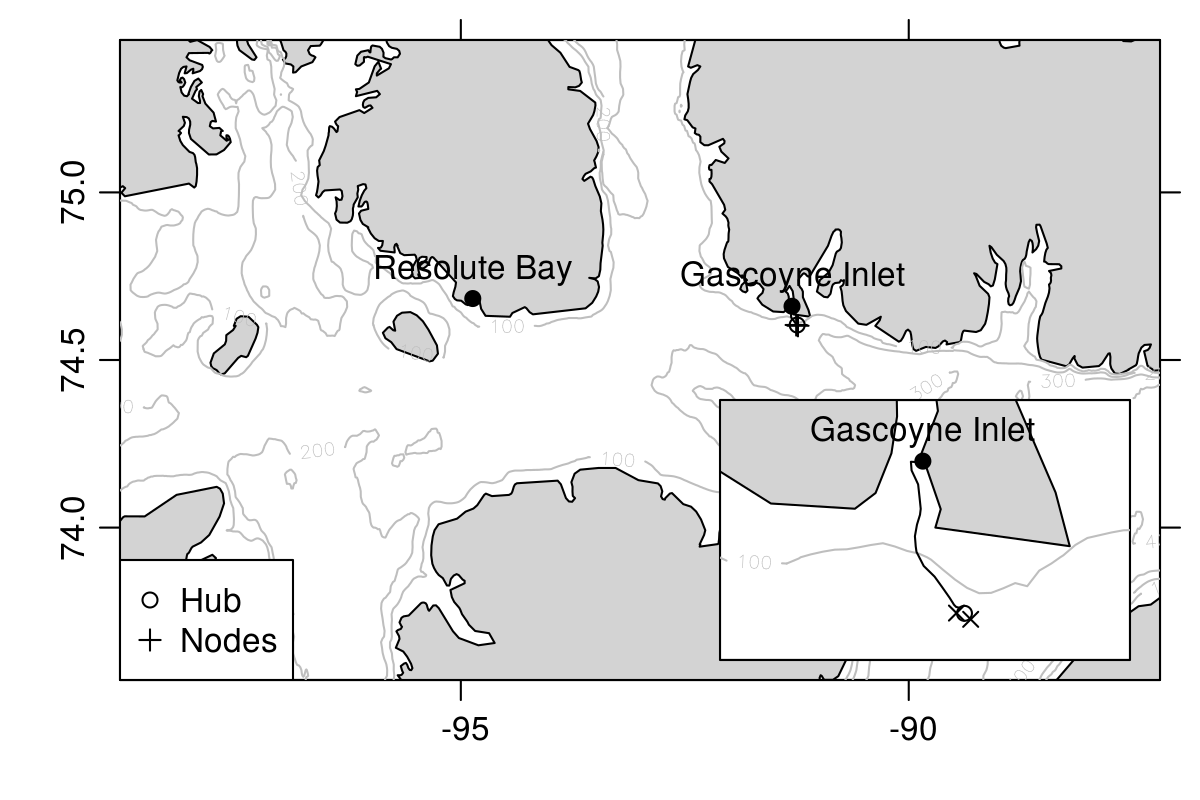
\includegraphics[width = 0.8\textwidth]{./figures/01_BSFieldSiteOverview.png}
\caption[Map of field site]{Map of the Barrow Strait field site showing the locations of the BSRTO hub and node moorings.}
\label{f:map}
\end{figure}



\begin{figure}
\centering
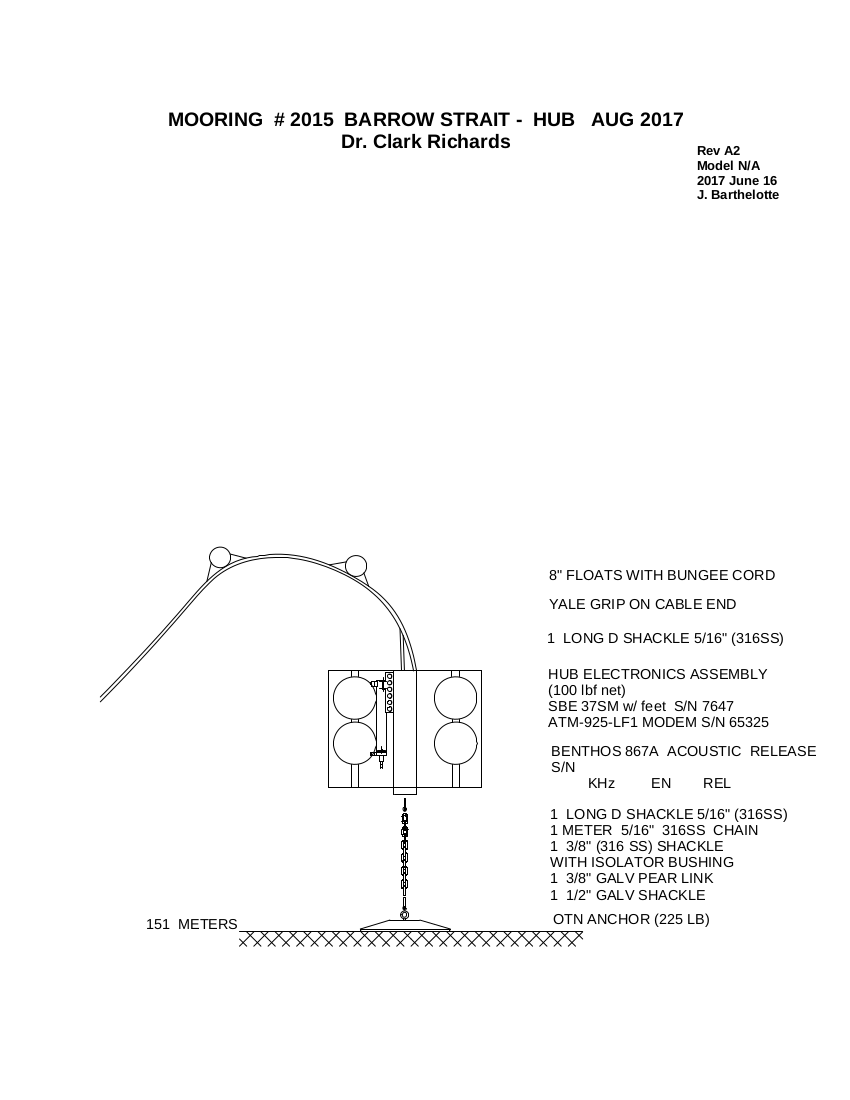
\includegraphics[width = 0.8\textwidth]{./figures/HUB.png}
\caption[Mooring Diagram: hub]{Diagram of the hub mooring.}
\label{f:md_hub}
\end{figure}

\begin{figure}
\centering
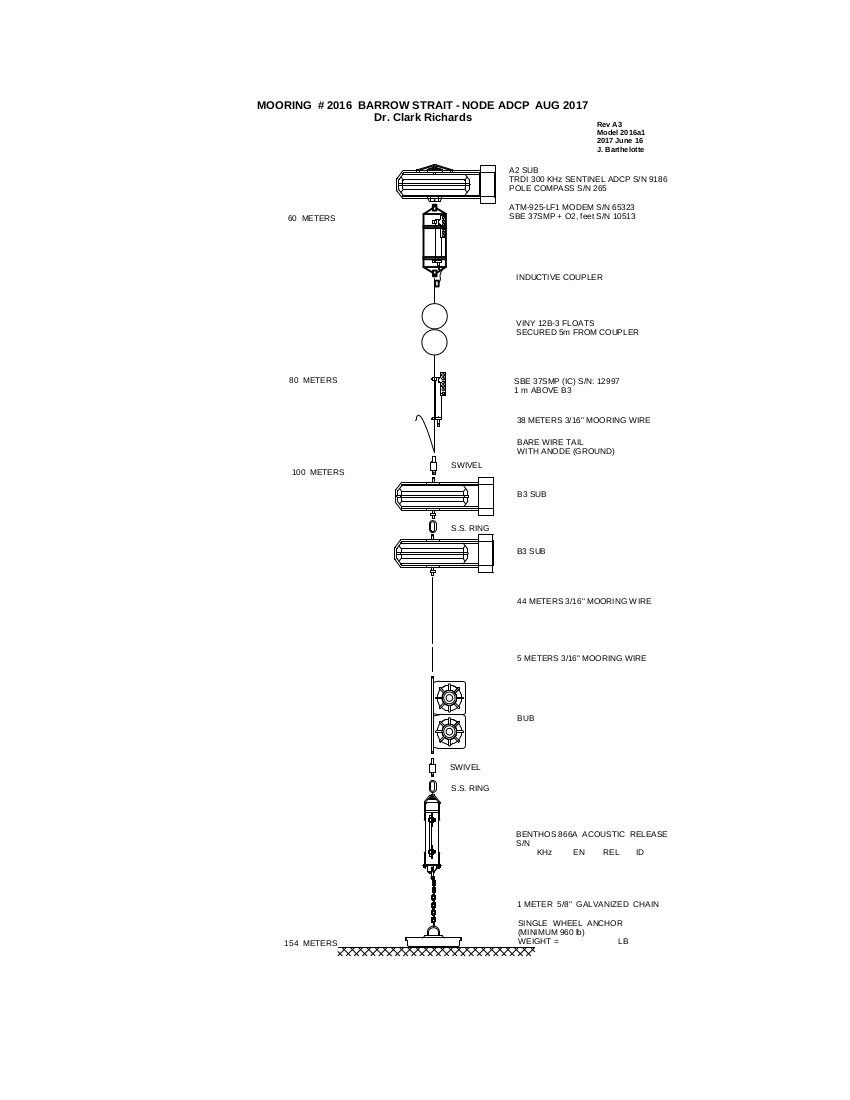
\includegraphics[width = 0.8\textwidth]{./figures/ADCP.png}
\caption[Mooring Diagram: ADCP node]{Diagram of the ADCP node mooring.}
\label{f:md_adcp}
\end{figure}

\begin{figure}
\centering
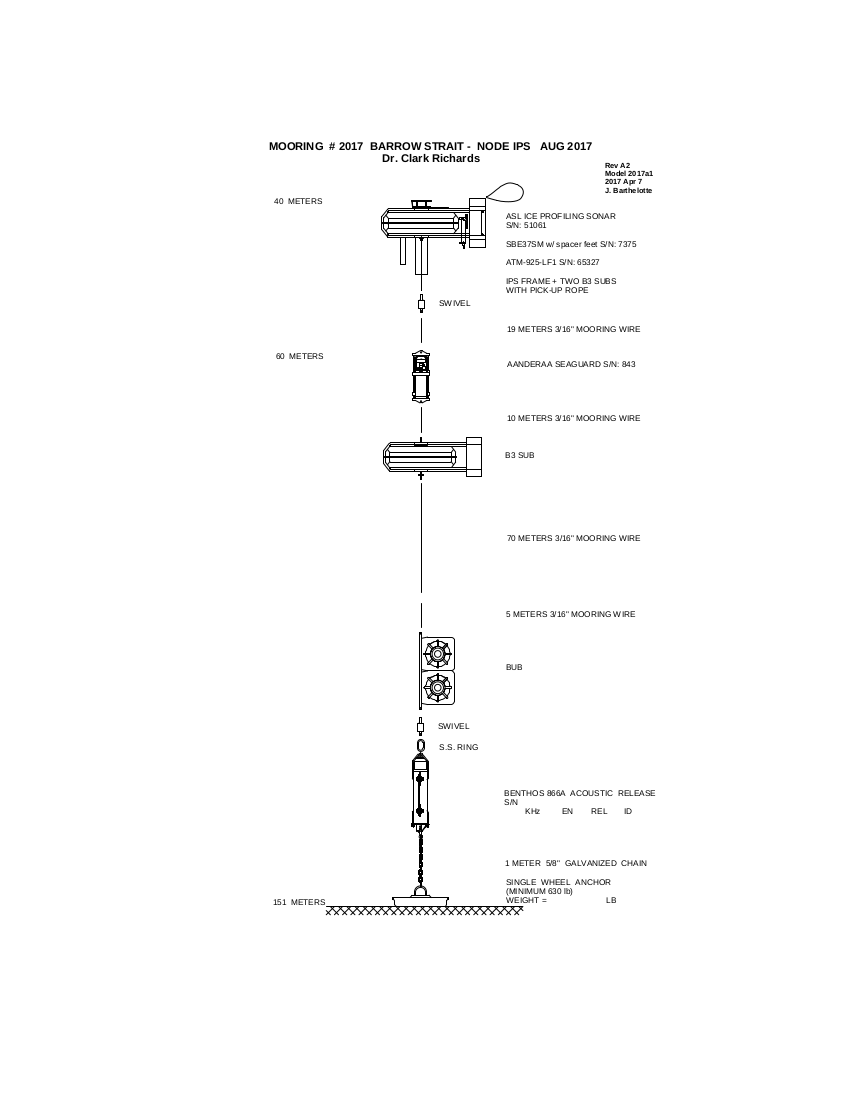
\includegraphics[width = 0.8\textwidth]{./figures/IPS.png}
\caption[Mooring Diagram: IPS node]{Diagram of the IPS node mooring.}
\label{f:md_ips}
\end{figure}



\begin{figure}
\centering
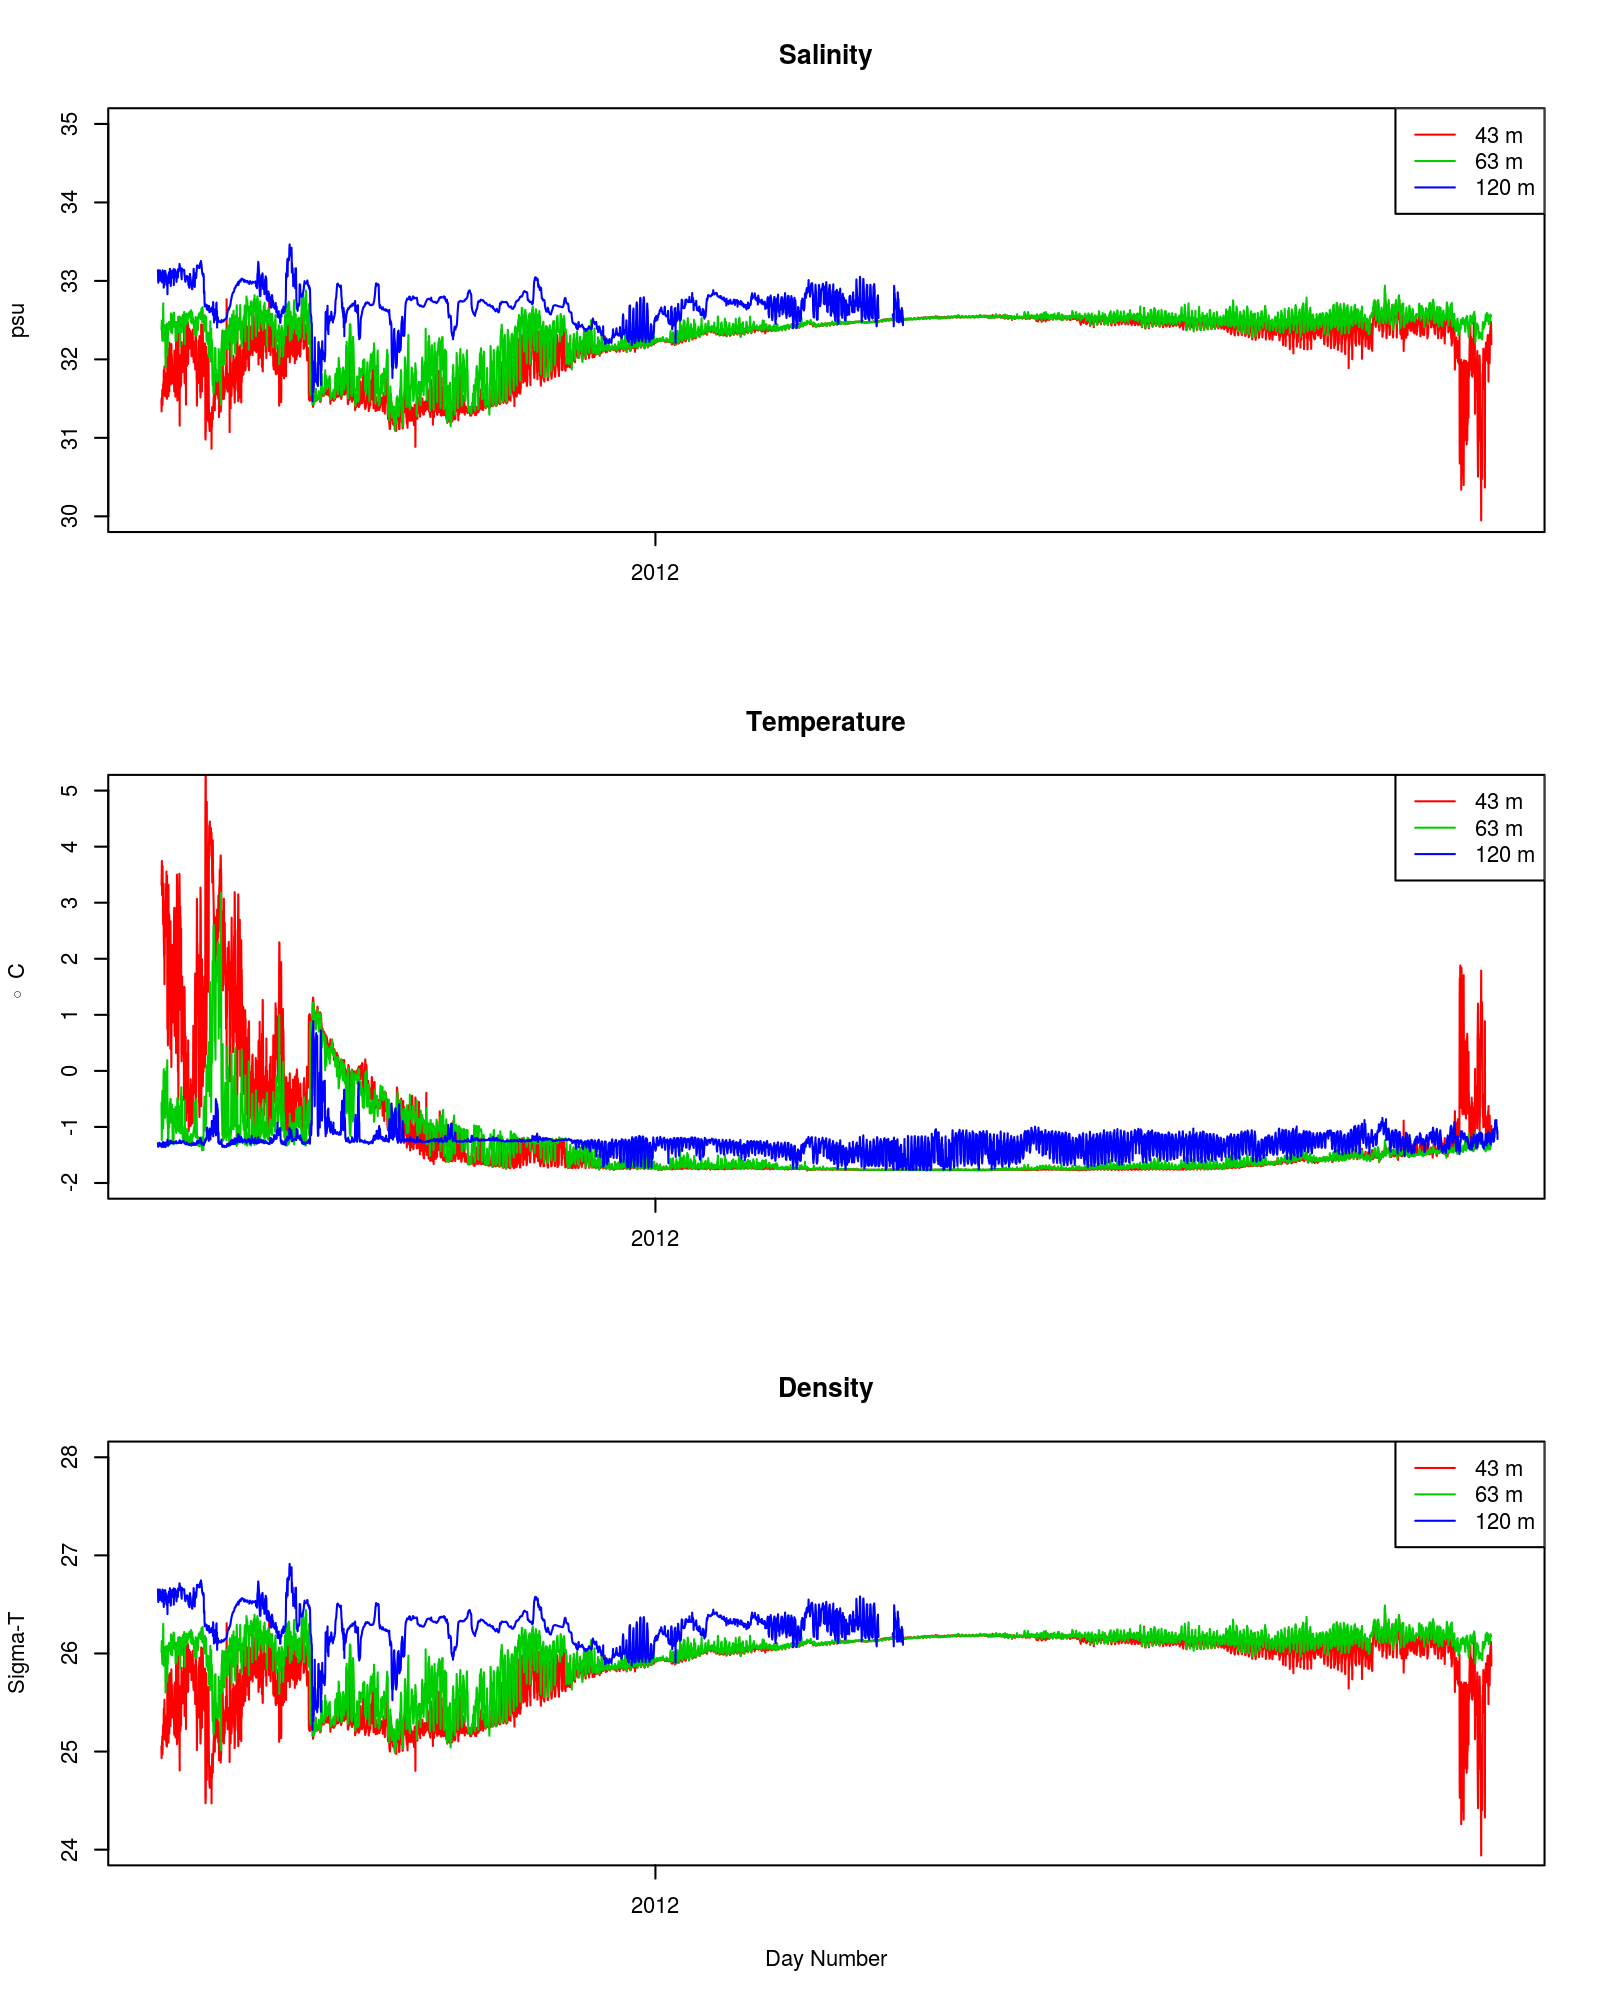
\includegraphics[width = 0.8\textwidth]{./figures/05_mctd_2011_2012.png}
\caption[Moored CTD, August 2011-2012]{Moored CTD data, August 2011 - August 2012.}
\label{f:mctd_2011_2012}
\end{figure}

\begin{figure}
\centering
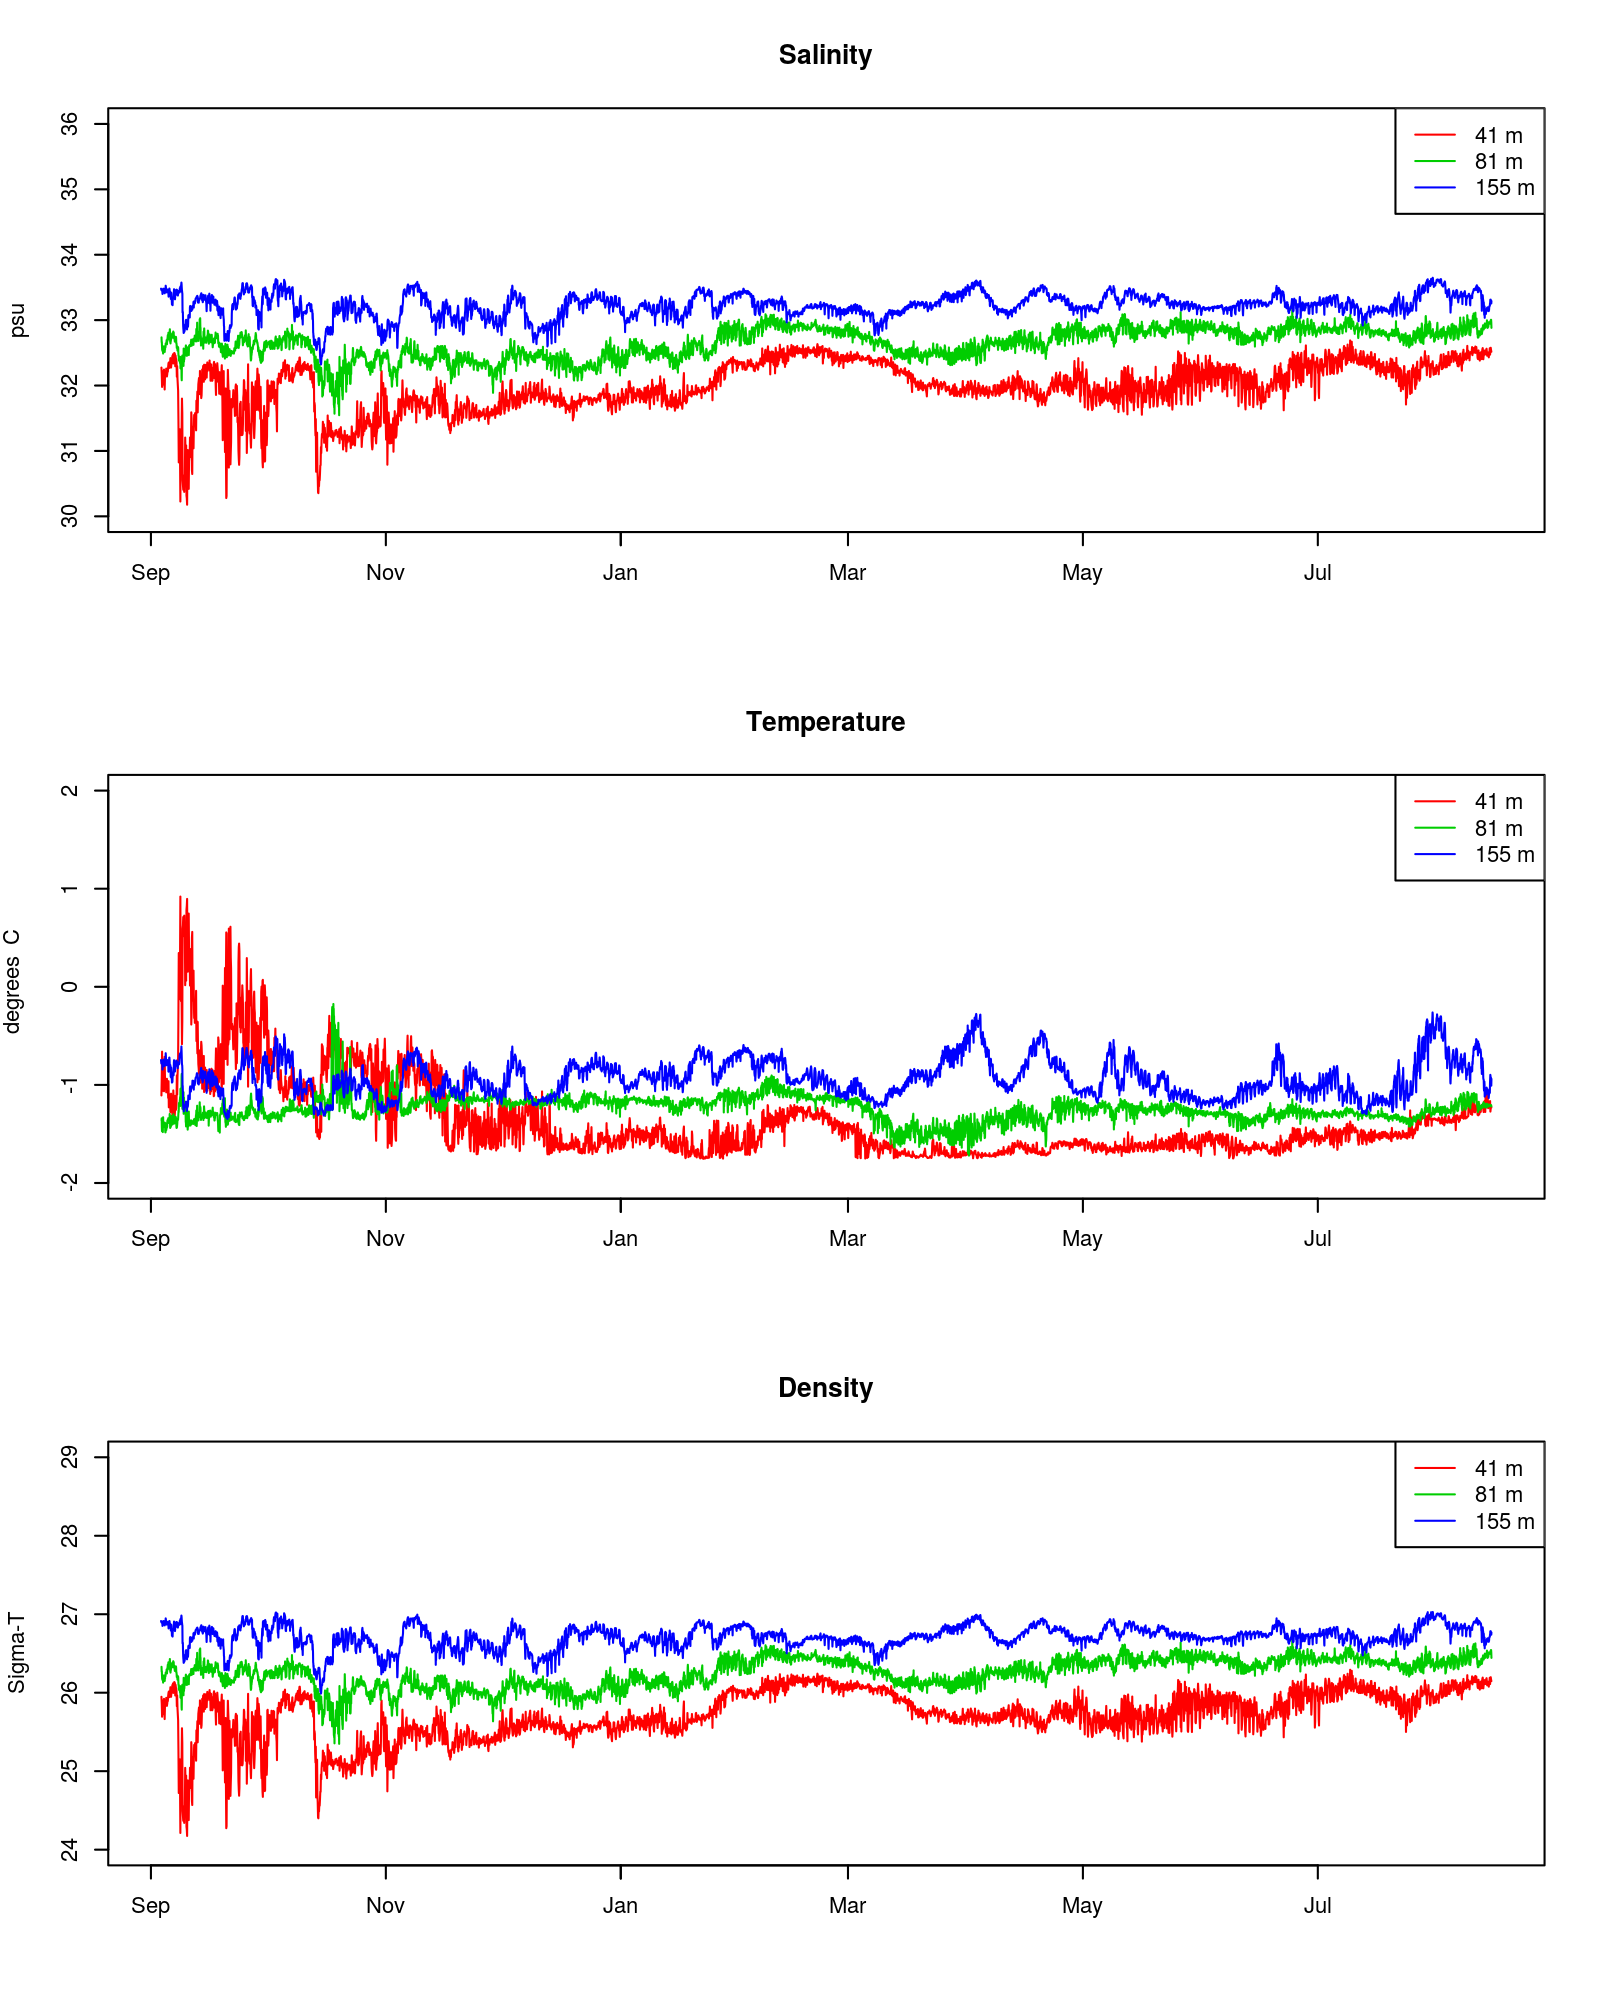
\includegraphics[width = 0.8\textwidth]{./figures/06_mctd_2012_2013.png}
\caption[Moored CTD, August 2012-2013]{Moored CTD data, August 2012 - August 2013.}
\label{f:mctd_2012_2013}
\end{figure}

\begin{figure}
\centering
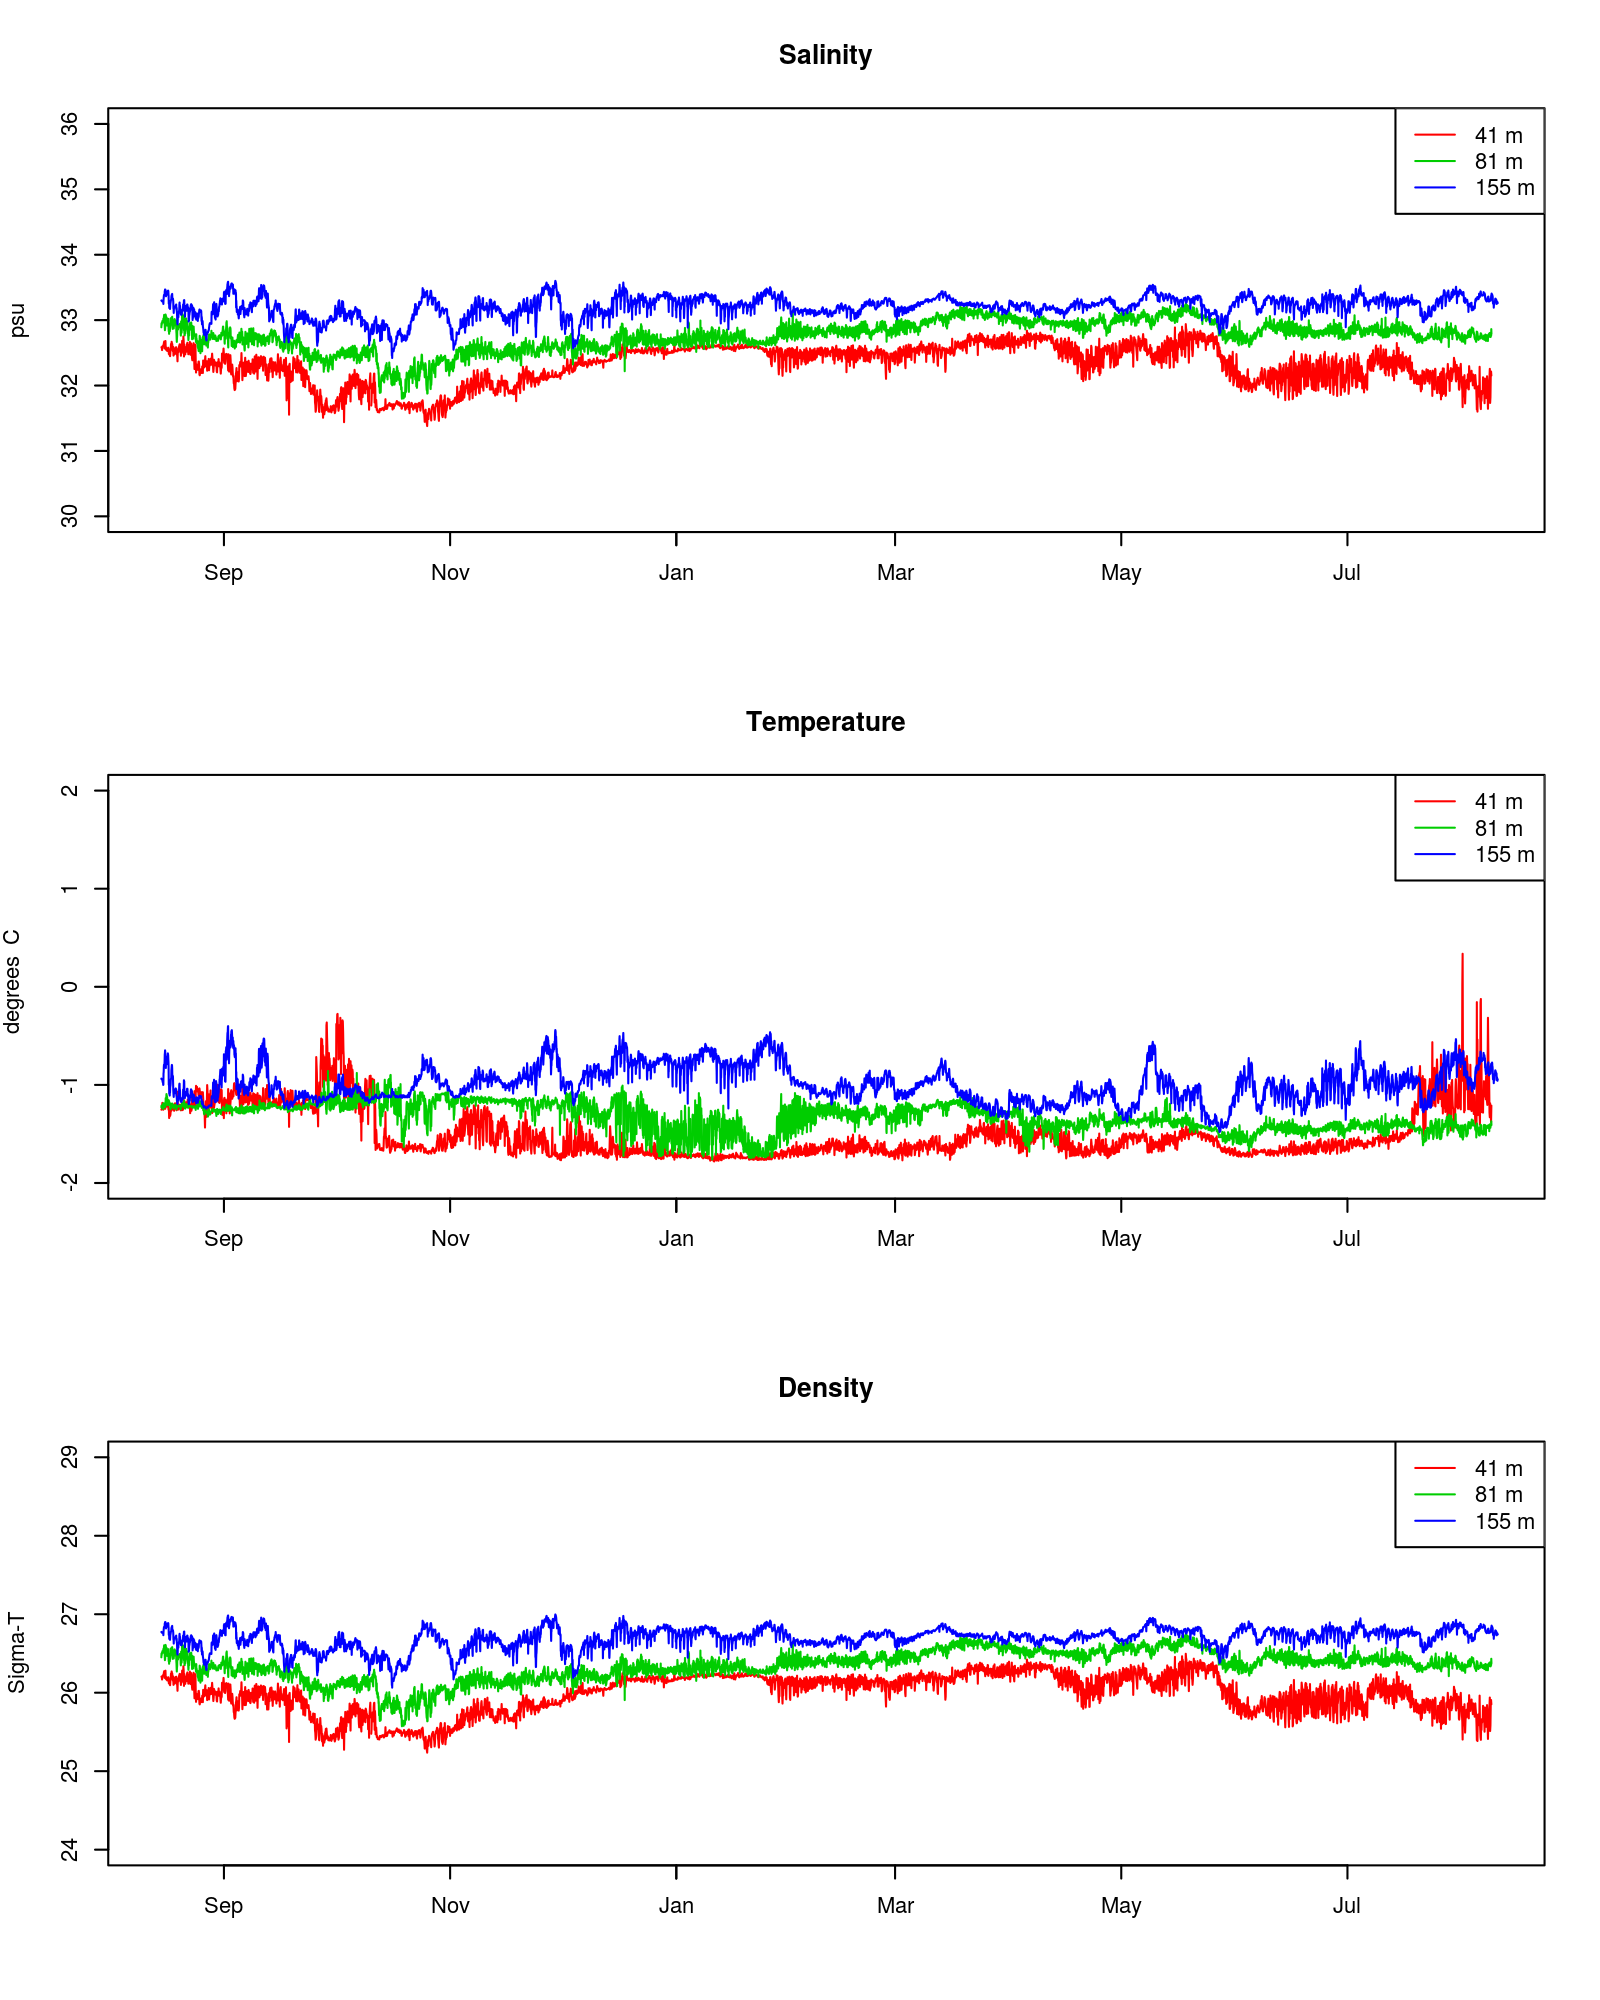
\includegraphics[width = 0.8\textwidth]{./figures/07_mctd_2013_2014.png}
\caption[Moored CTD, August 2013-2014]{Moored CTD data, August 2013 - August 2014.}
\label{f:mctd_2013_2014}
\end{figure}

\begin{figure}
\centering
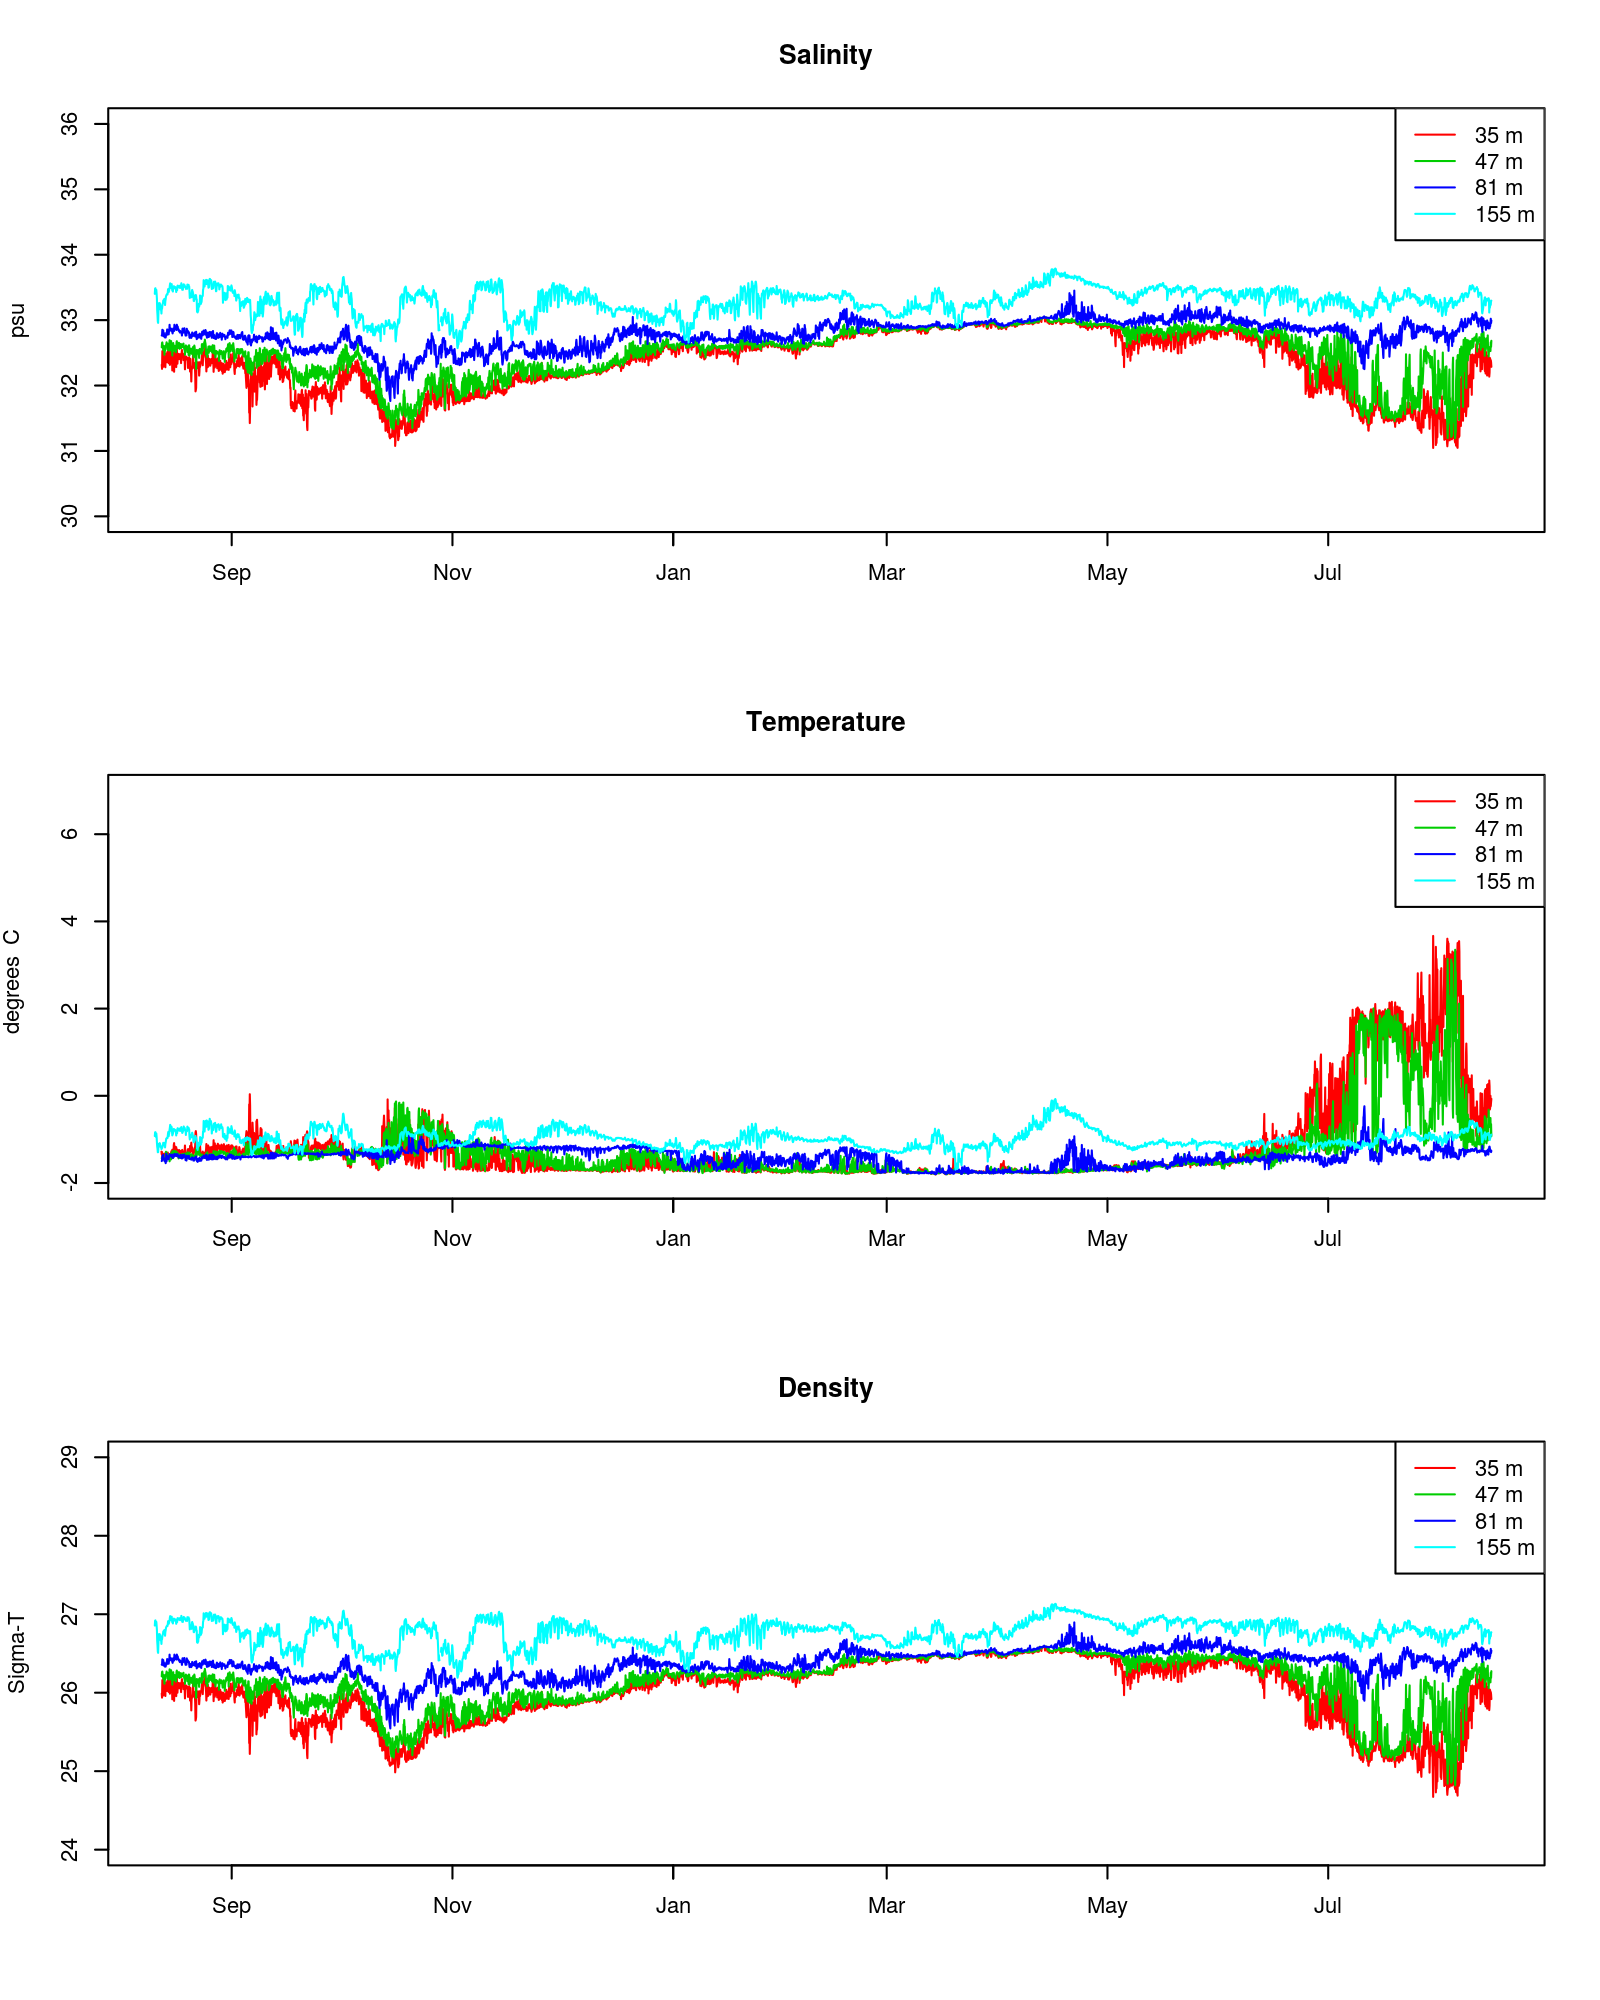
\includegraphics[width = 0.8\textwidth]{./figures/08_mctd_2014_2015.png}
\caption[Moored CTD, August 2014-2015]{Moored CTD data, August 2014 - August 2015.}
\label{f:mctd_2014_2015}
\end{figure}

\begin{figure}
\centering
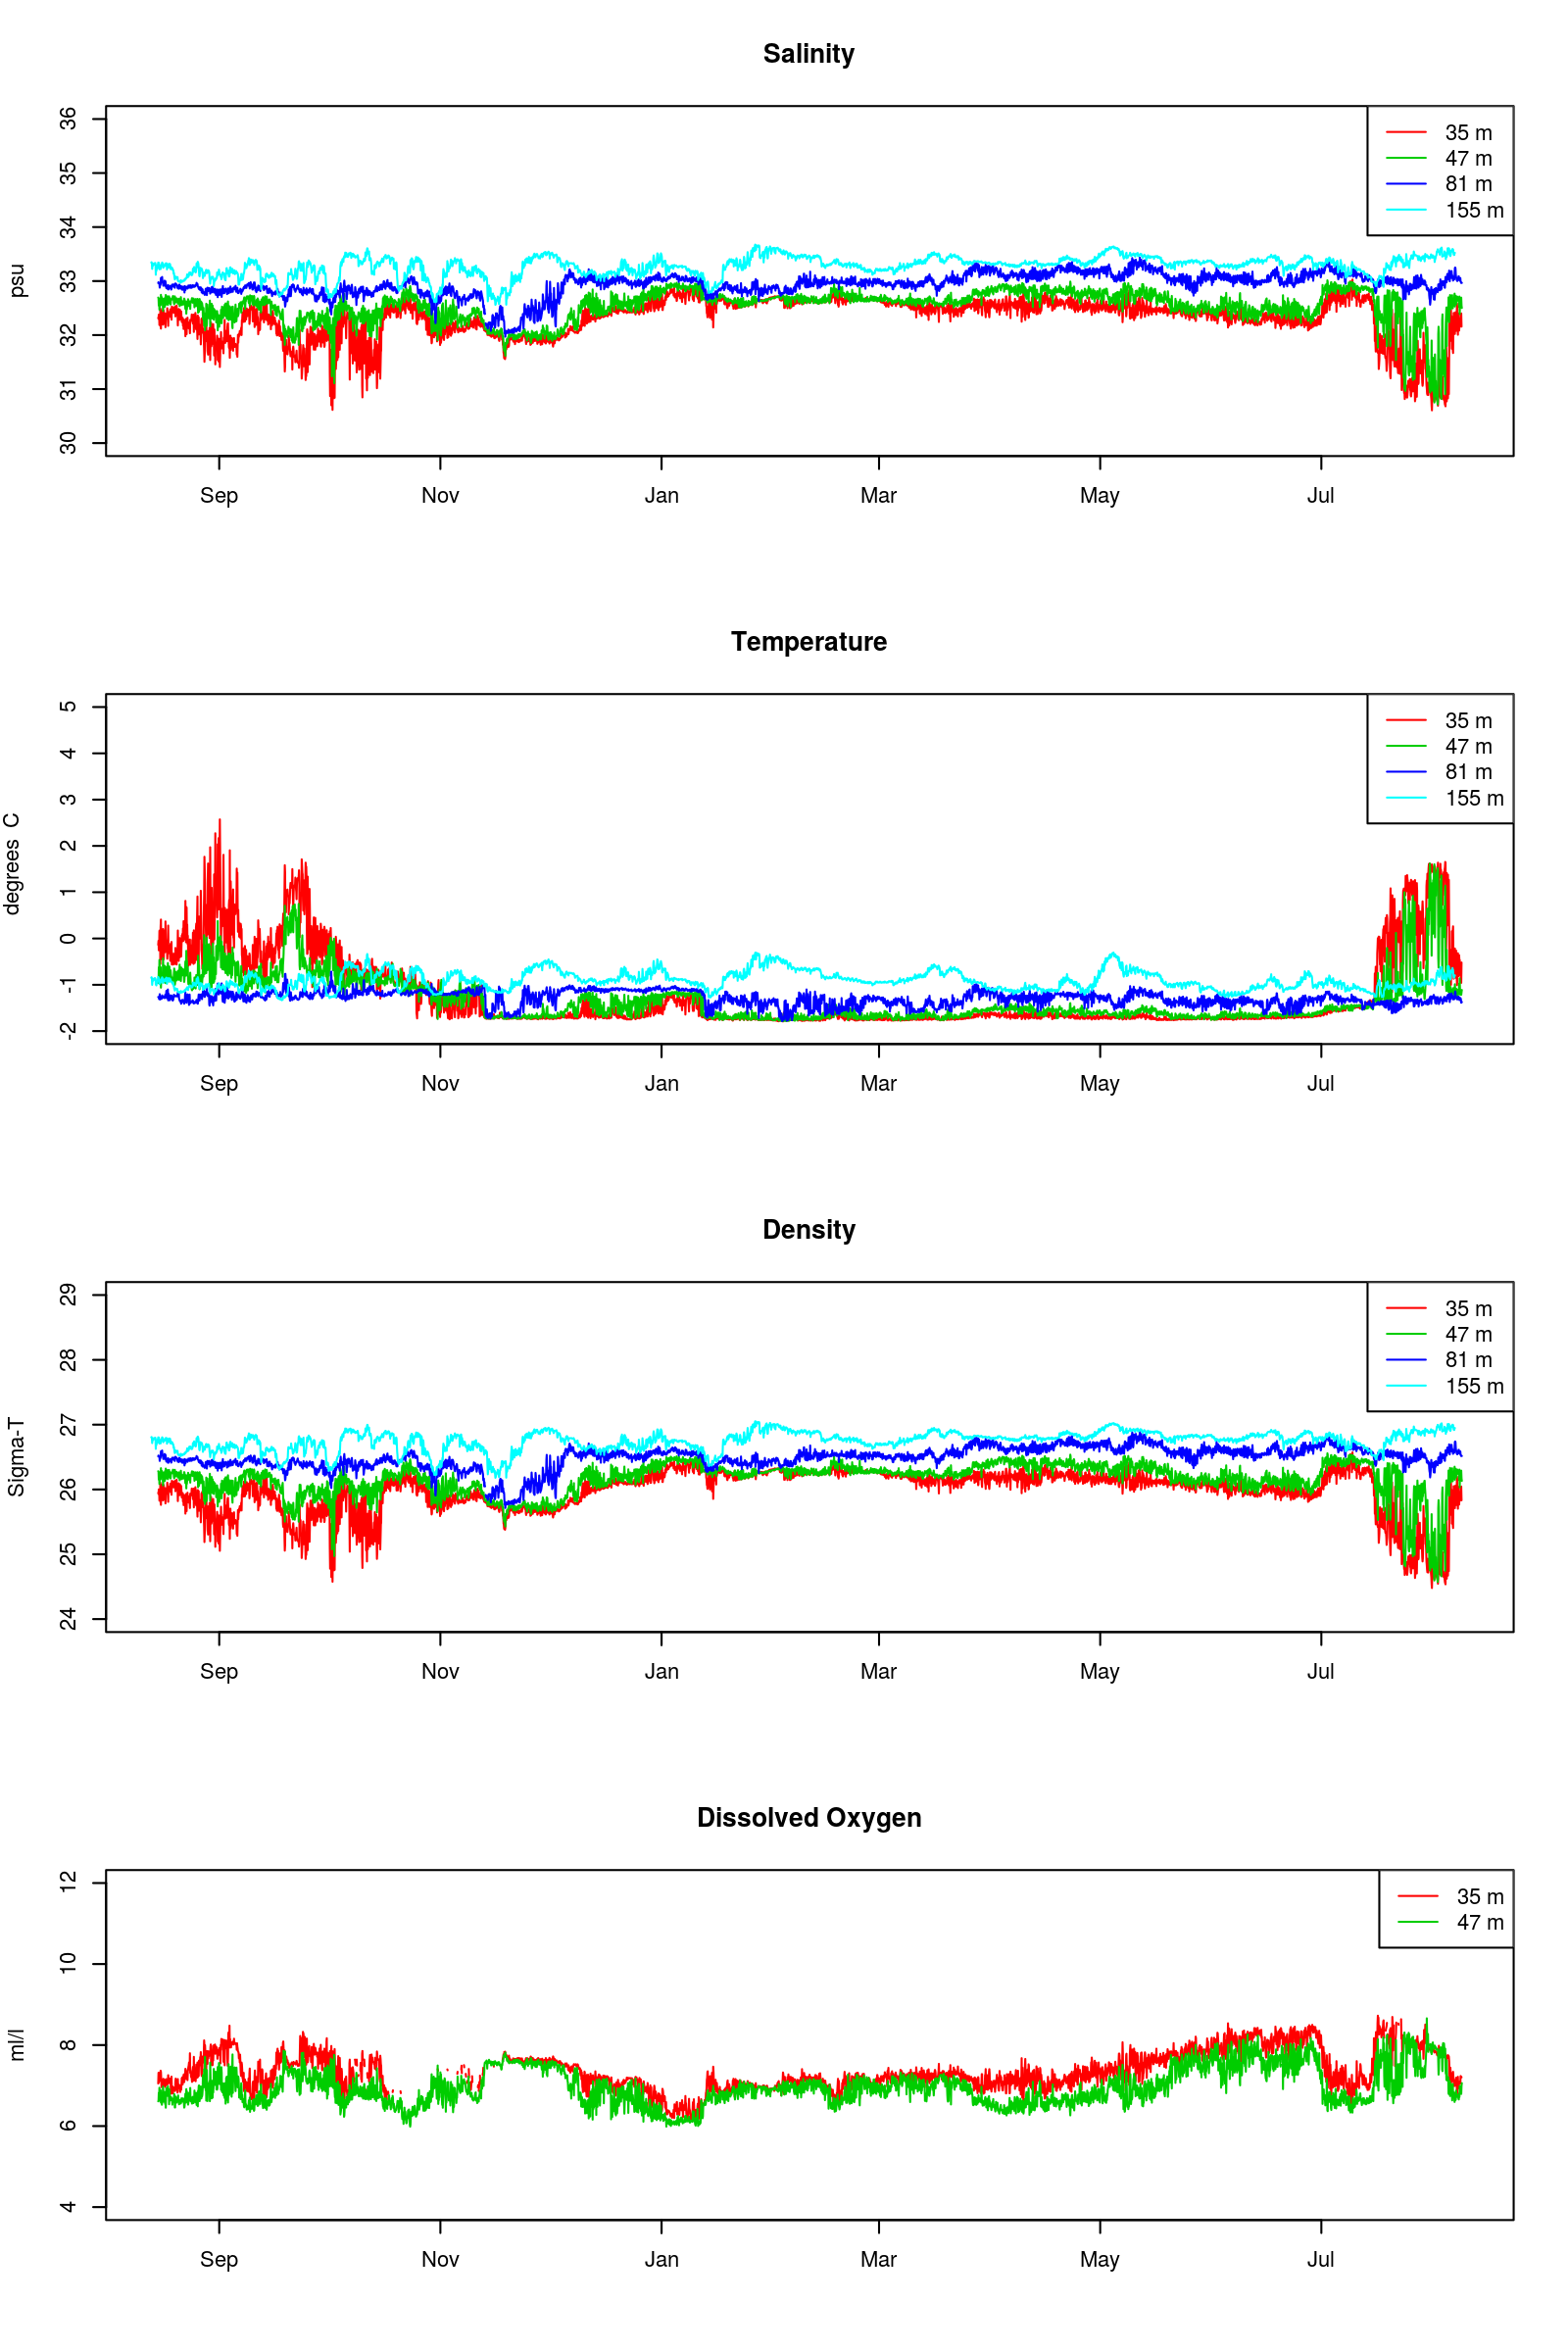
\includegraphics[width = 0.8\textwidth]{./figures/09_mctd_2015_2016.png}
\caption[Moored CTD, August 2015-2016]{Moored CTD data, August 2015 - August 2016.}
\label{f:mctd_2015_2016}
\end{figure}




\begin{figure}  
\centering
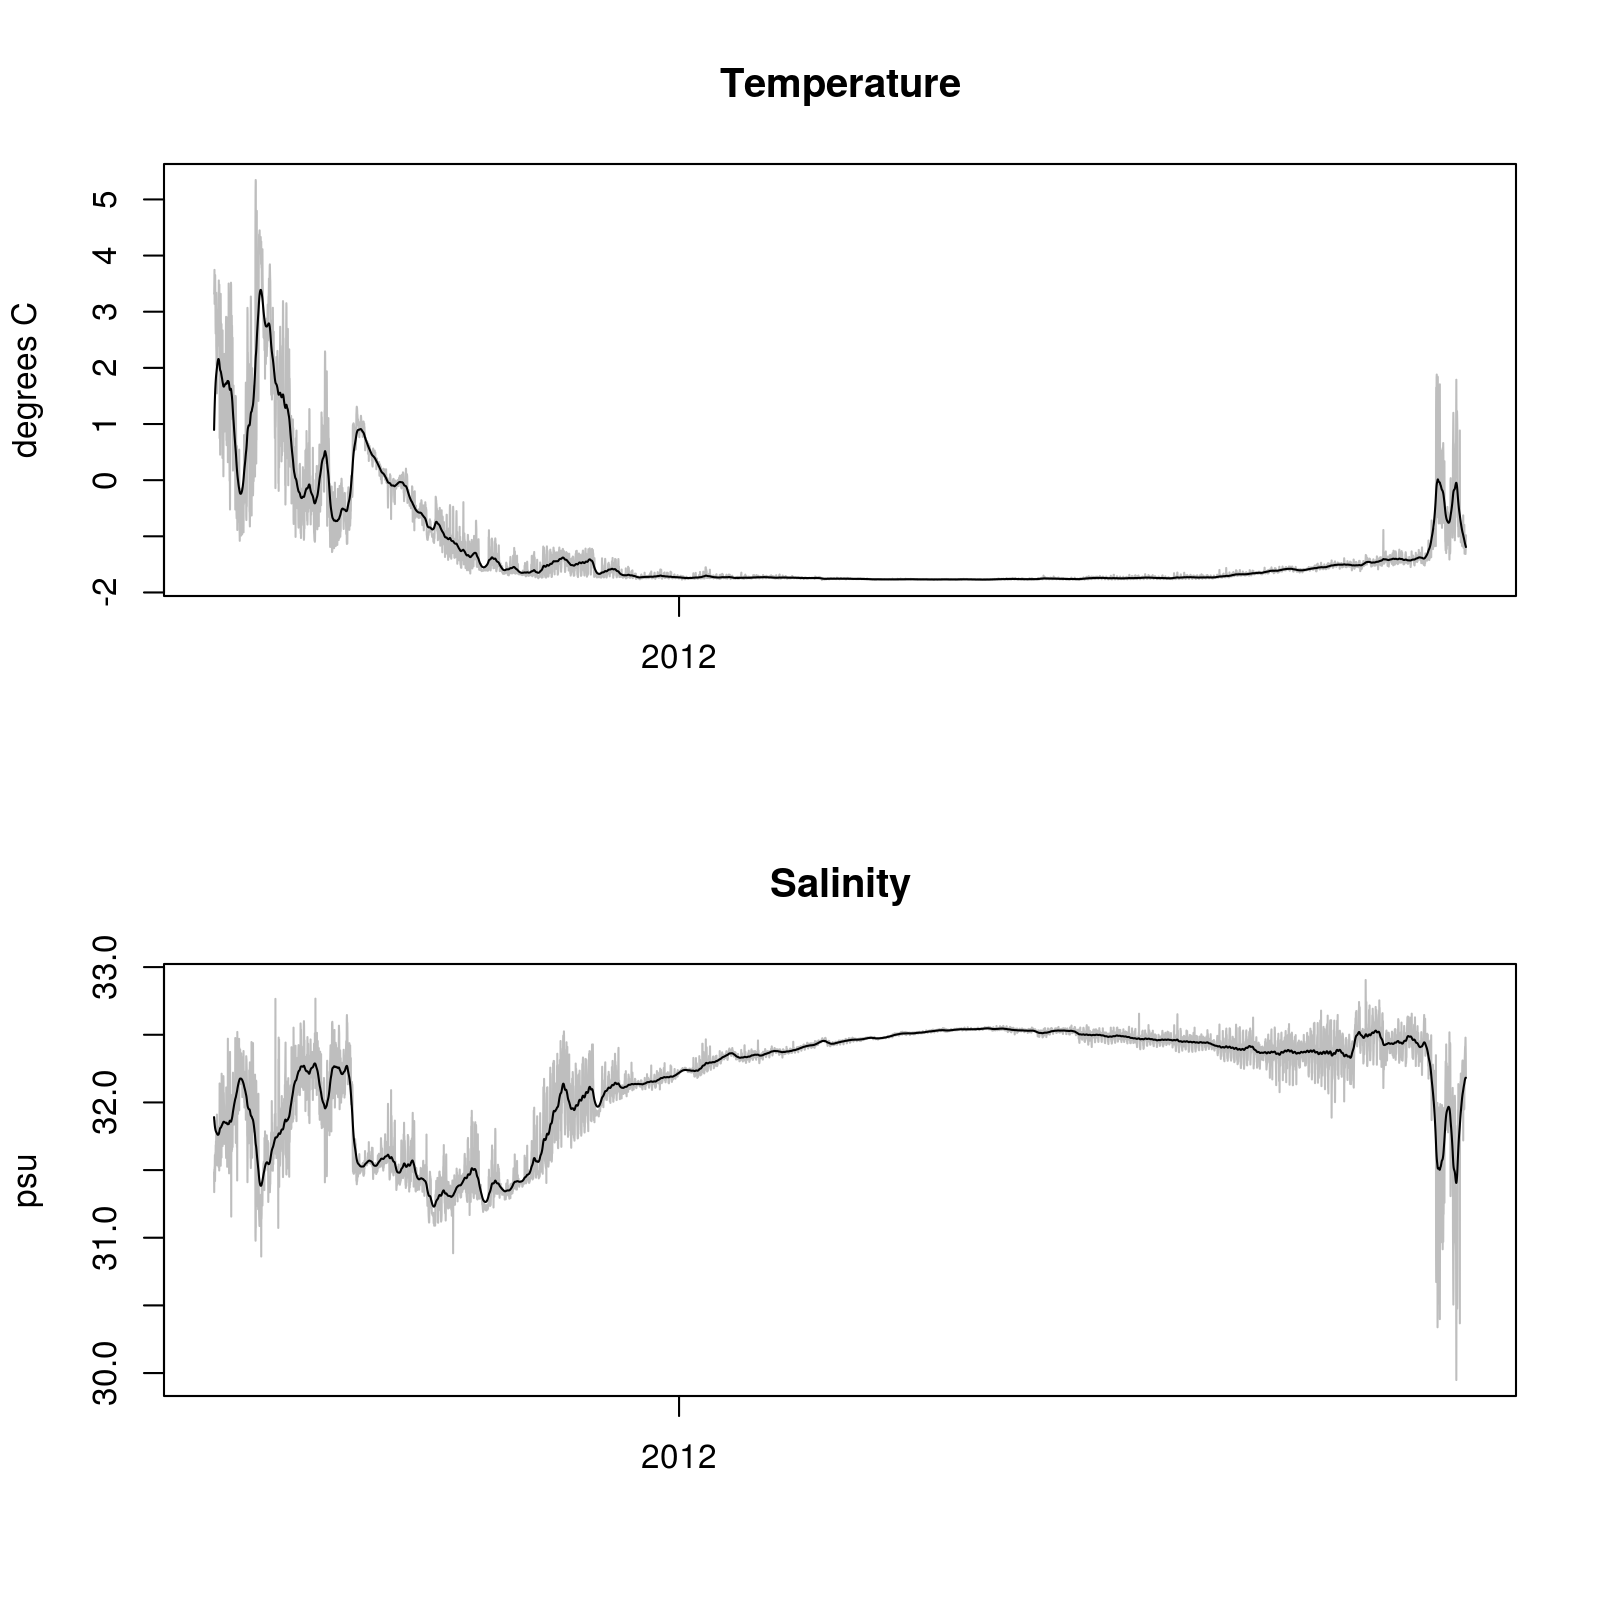
\includegraphics[width = 0.8\textwidth]{./figures/19_lpf_TS_43m_2011_2012.png}
\caption[Low-pass filtered T, S (43 m), 2011-2012]{Low-pass filtered T, S (43 m), August 2011 - August 2012}
\label{f:ctd_43_lpf_2011_2012}
\end{figure}

\begin{figure}  
\centering
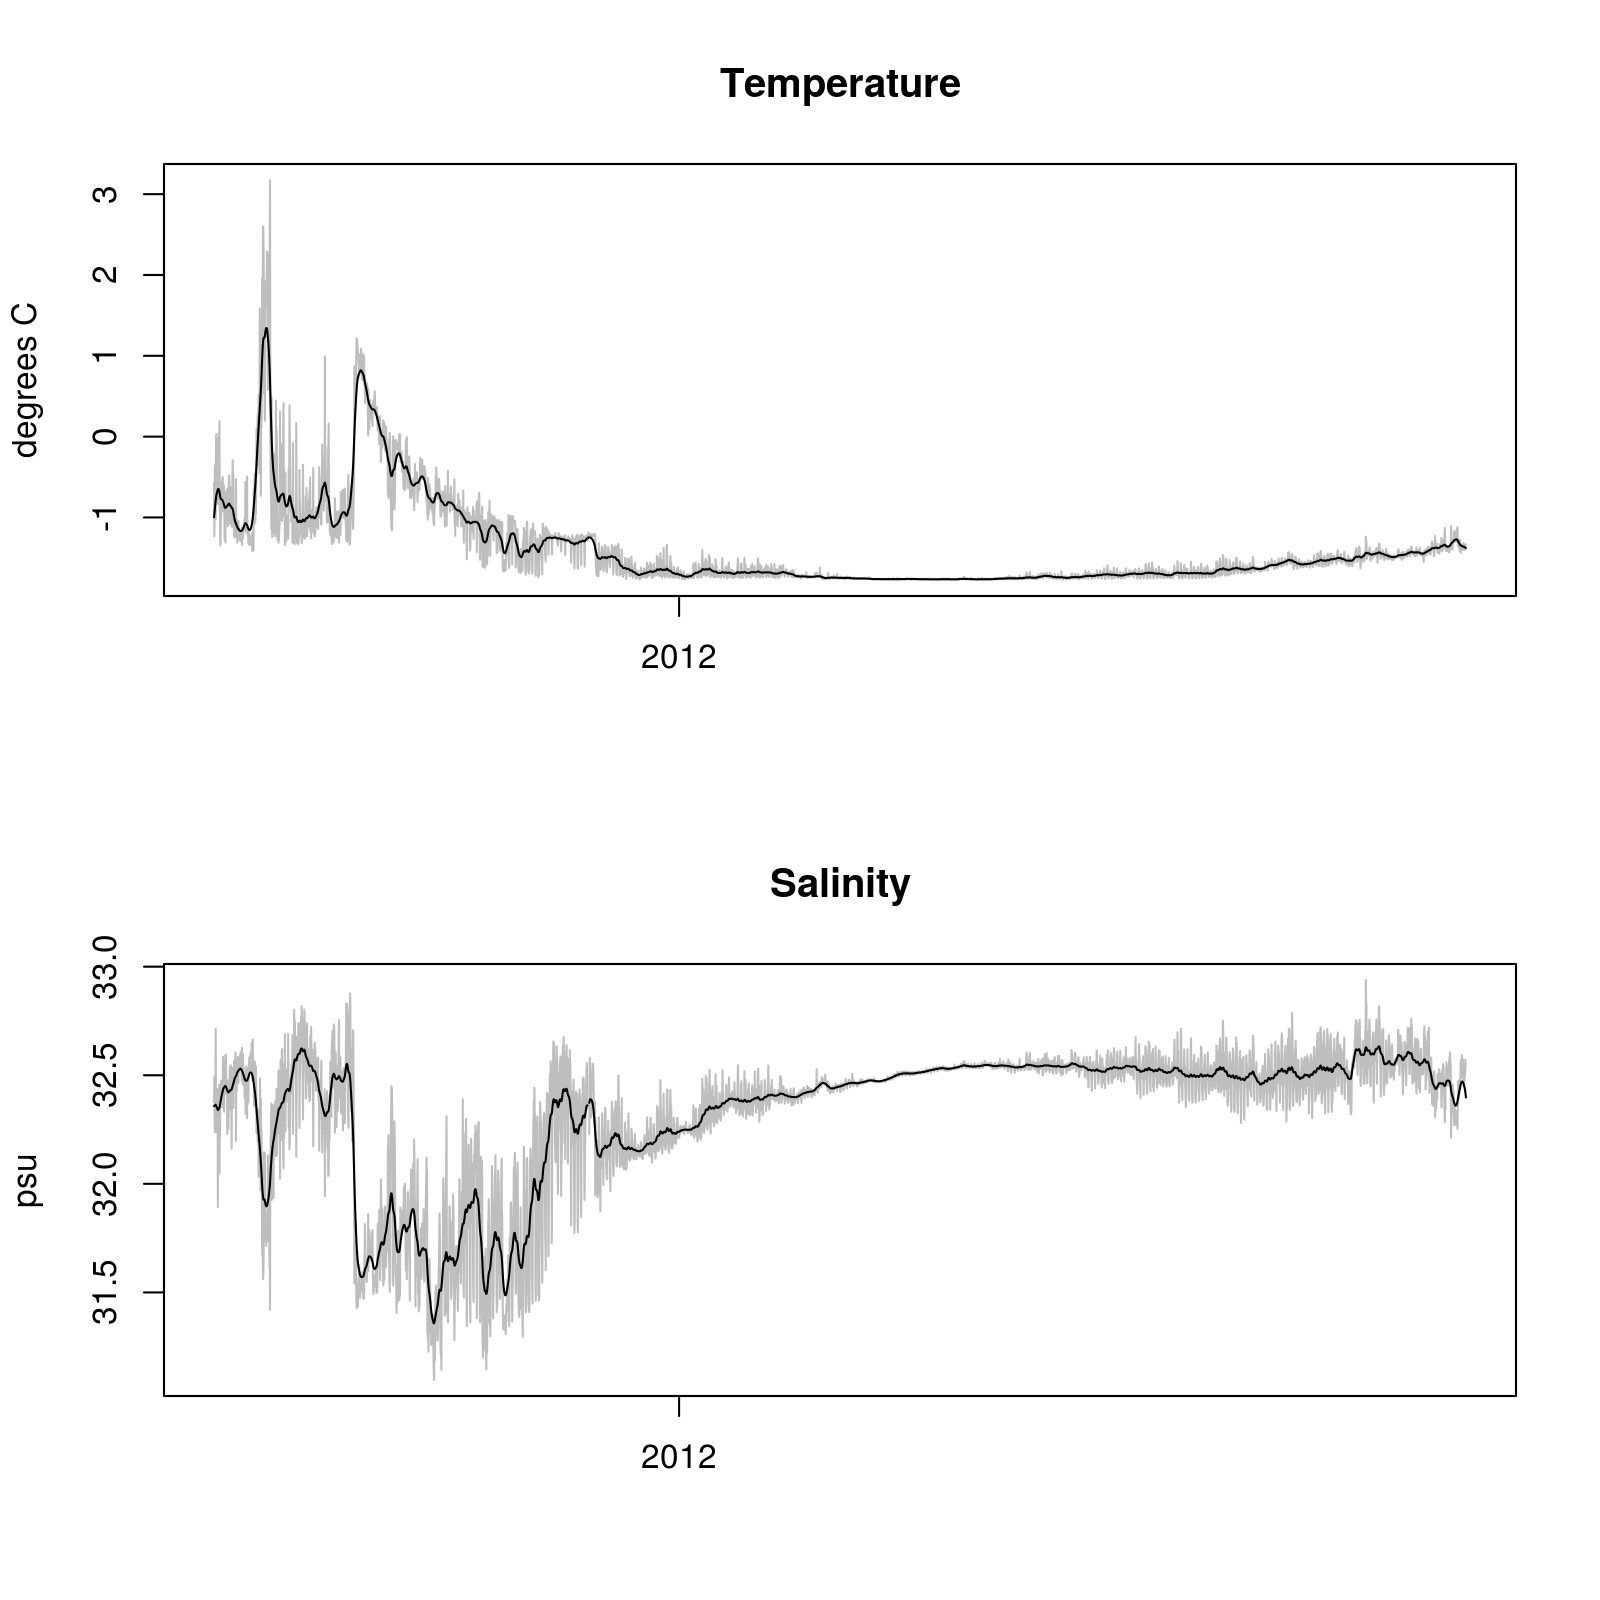
\includegraphics[width = 0.8\textwidth]{./figures/20_lpf_TS_63m_2011_2012.png}
\caption[Low-pass filtered T, S (63 m), 2011-2012]{Low-pass filtered T, S (63 m), August 2011 - August 2012}
\label{f:ctd_63_lpf_2011_2012}
\end{figure}

\begin{figure}  
\centering
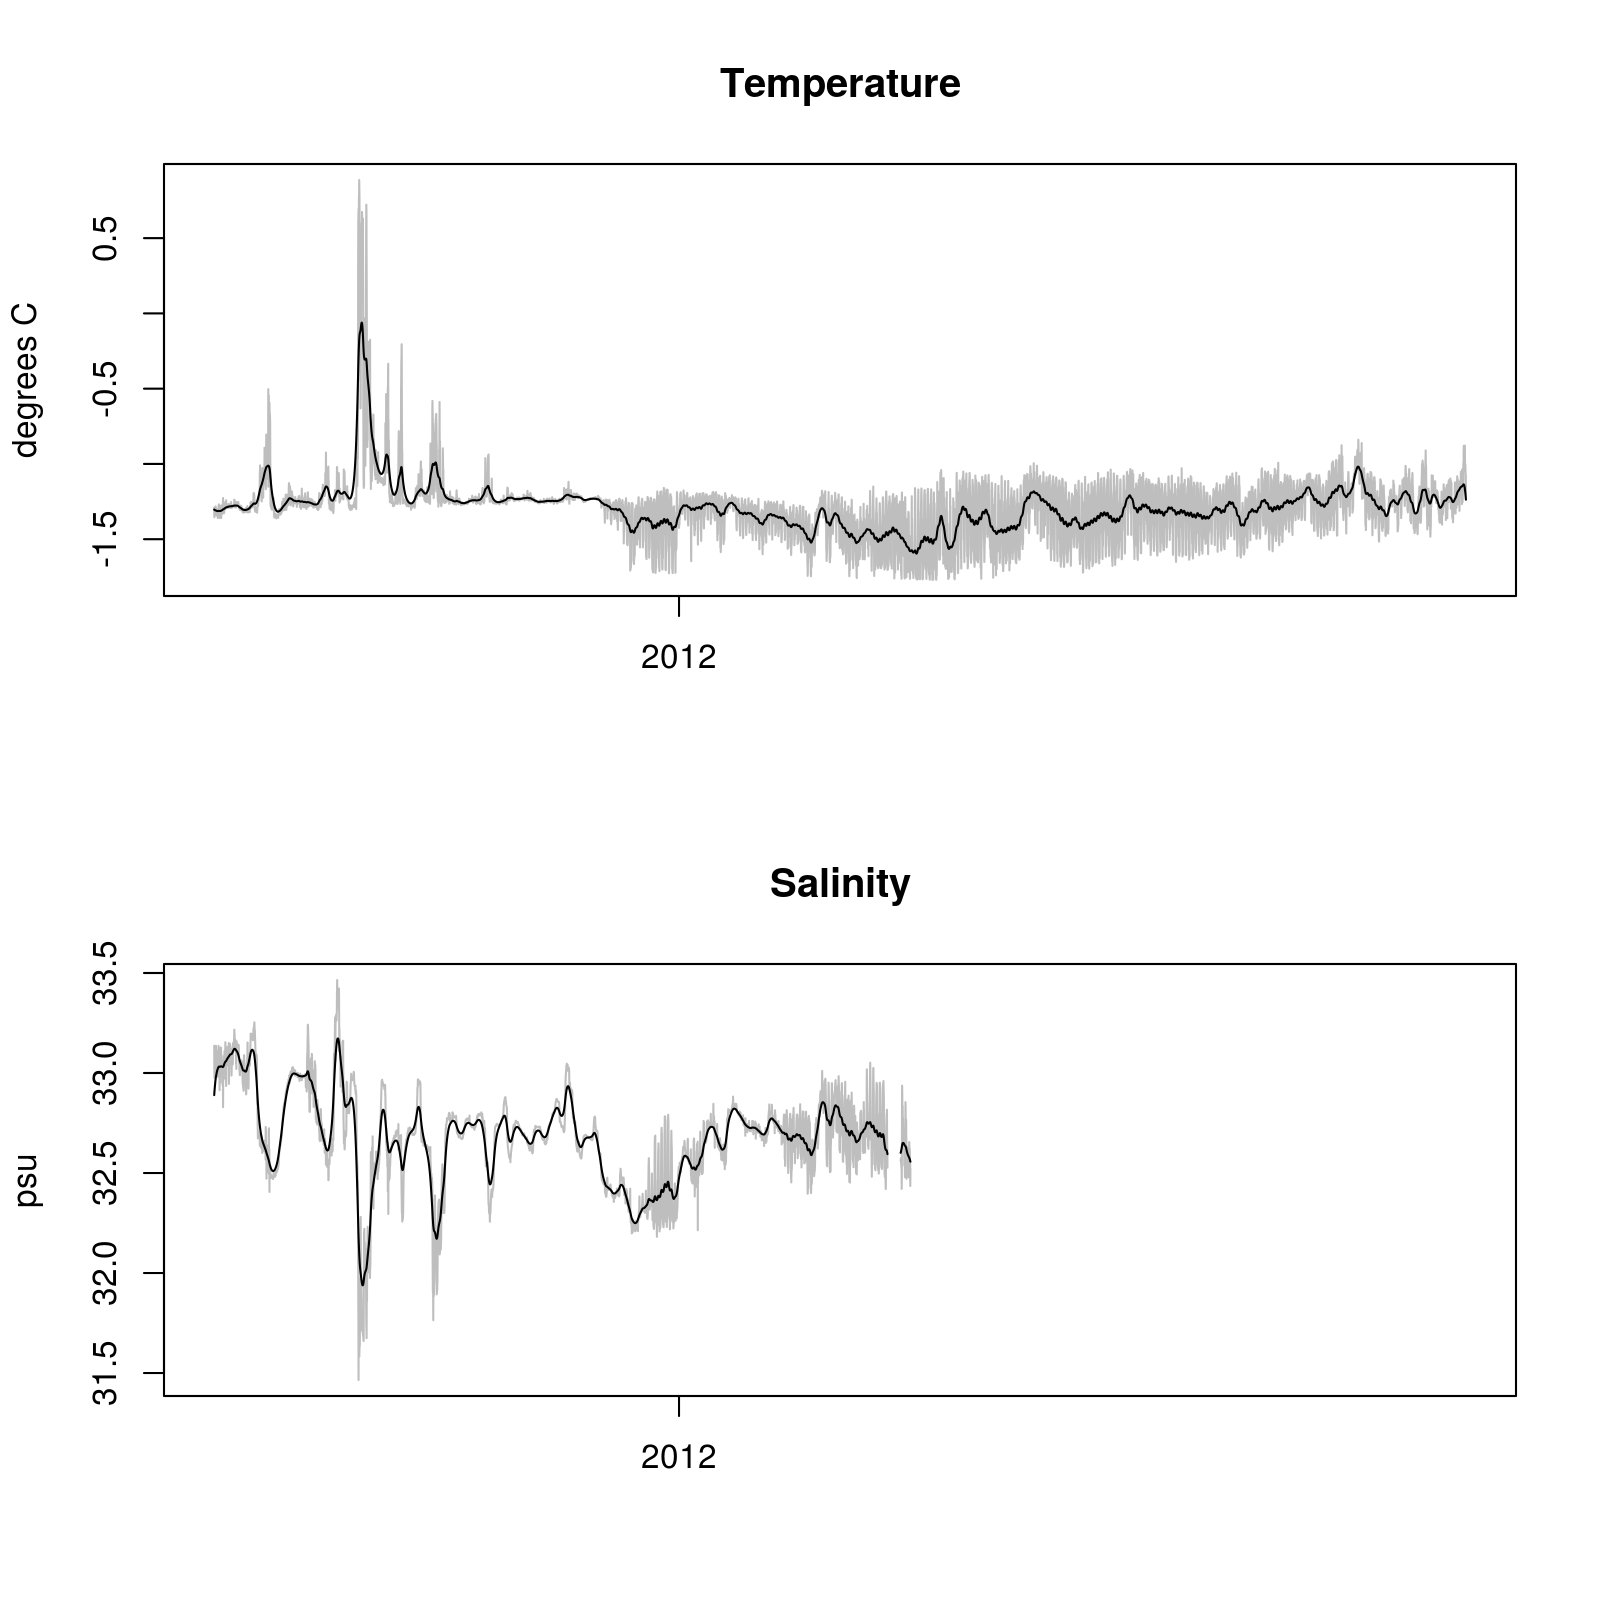
\includegraphics[width = 0.8\textwidth]{./figures/21_lpf_TS_120m_2011_2012.png}
\caption[Low-pass filtered T, S (120 m), 2011-2012]{Low-pass filtered T, S (120 m), August 2011 - August 2012}
\label{f:ctd_120_lpf_2011_2012}
\end{figure}


\begin{figure}  
\centering
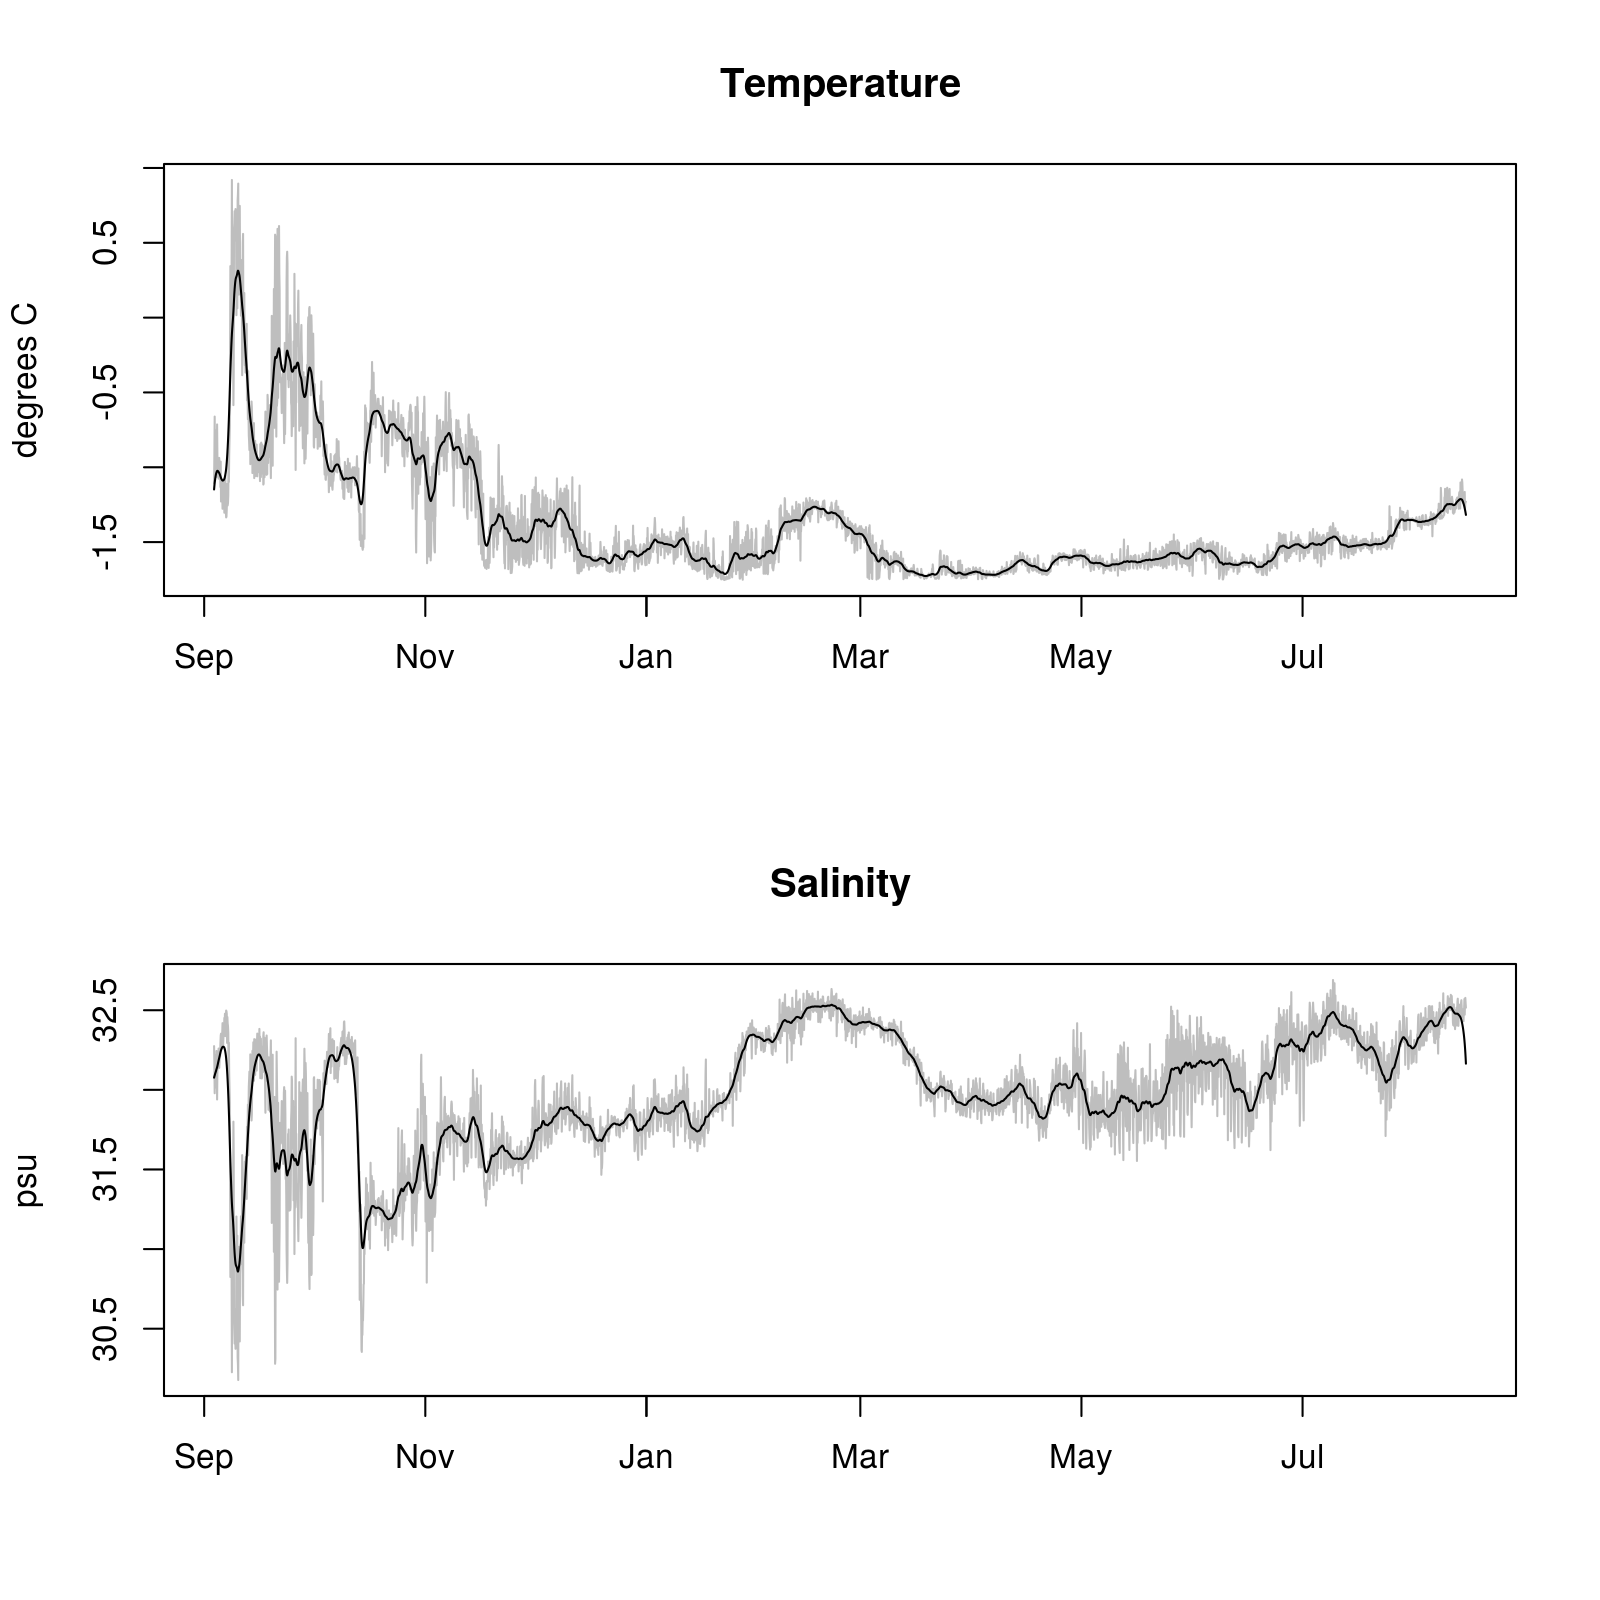
\includegraphics[width = 0.8\textwidth]{./figures/22_lpf_TS_41m_2012_2013.png}
\caption[Low-pass filtered T, S (41 m), 2012-2013]{Low-pass filtered T, S (41 m), August 2012 - August 2013}
\label{f:ctd_41_lpf_2012_2013}
\end{figure}

\begin{figure}  
\centering
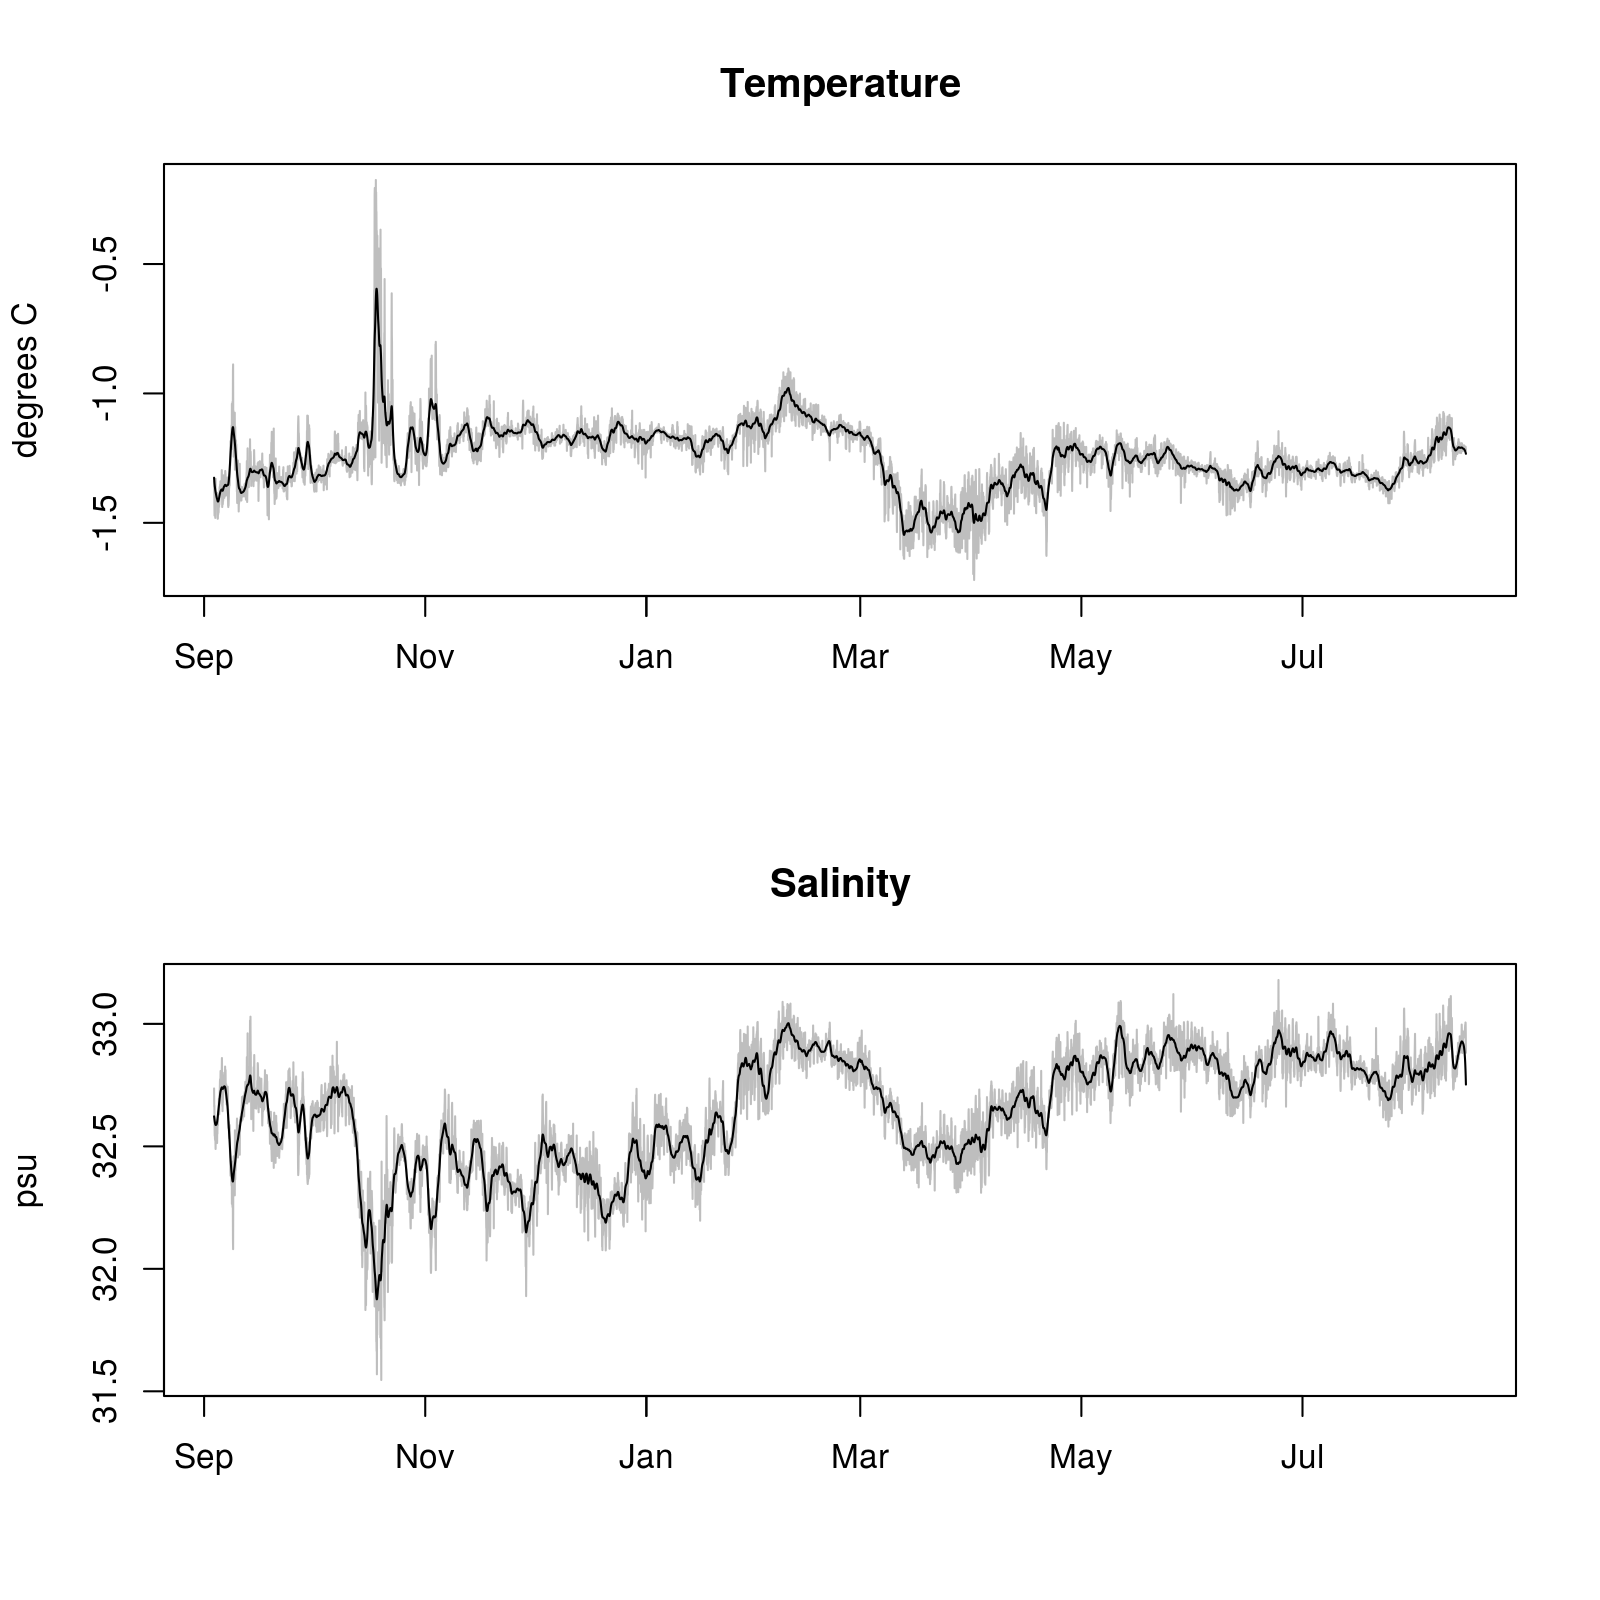
\includegraphics[width = 0.8\textwidth]{./figures/23_lpf_TS_81m_2012_2013.png}
\caption[Low-pass filtered T, S (81 m), 2012-2013]{Low-pass filtered T, S (81 m), August 2012 - August 2013}
\label{f:ctd_81_lpf_2012_2013}
\end{figure}

\begin{figure}  
\centering
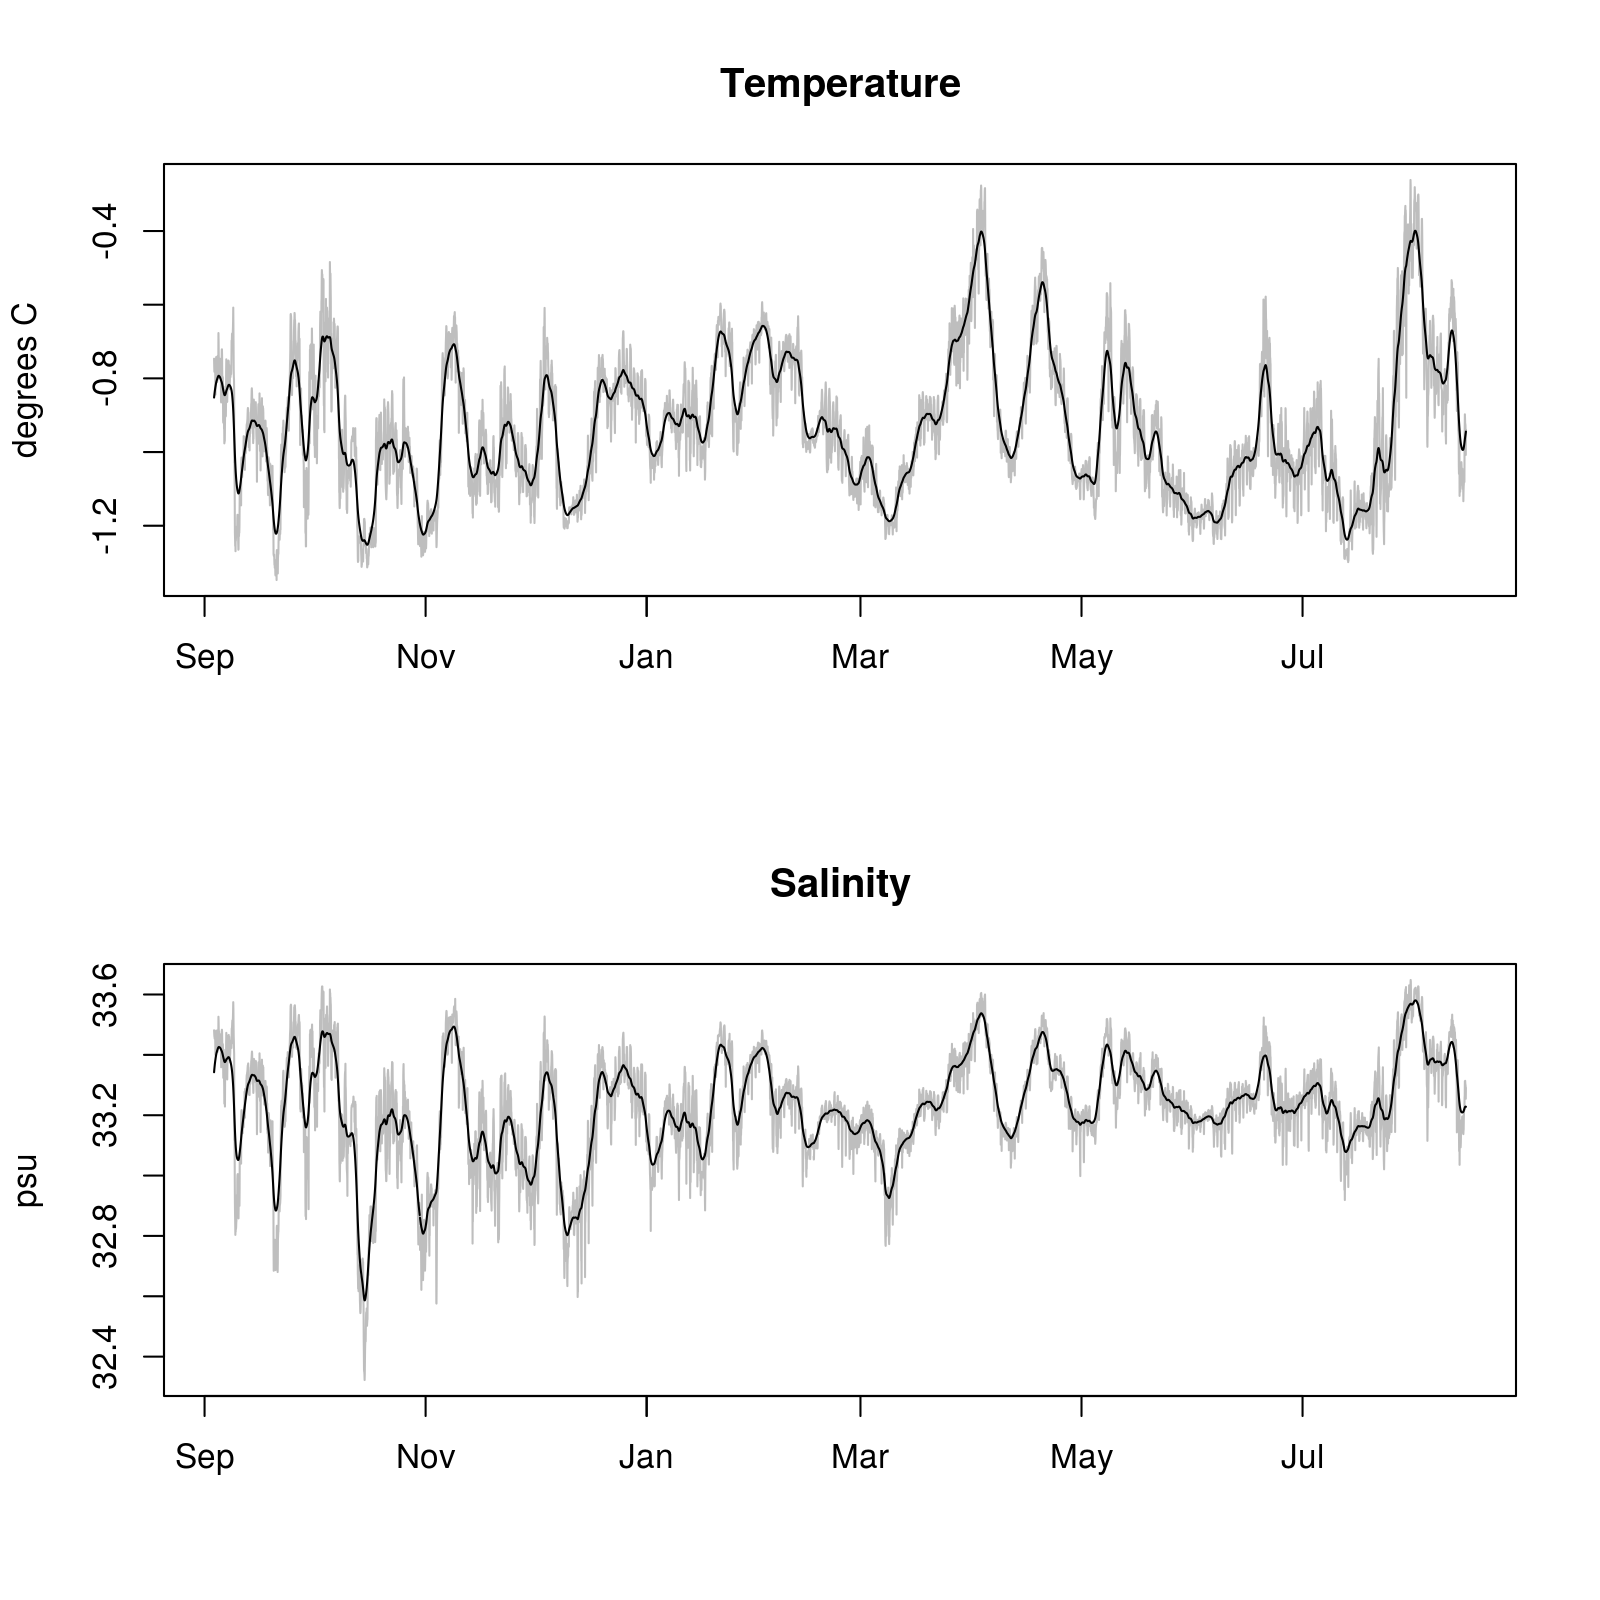
\includegraphics[width = 0.8\textwidth]{./figures/24_lpf_TS_155m_2012_2013.png}
\caption[Low-pass filtered T, S (155 m), 2012-2013]{Low-pass filtered T, S (155 m), August 2012 - August 2013}
\label{f:ctd_155_lpf_2012_2013}
\end{figure}


\begin{figure}  
\centering
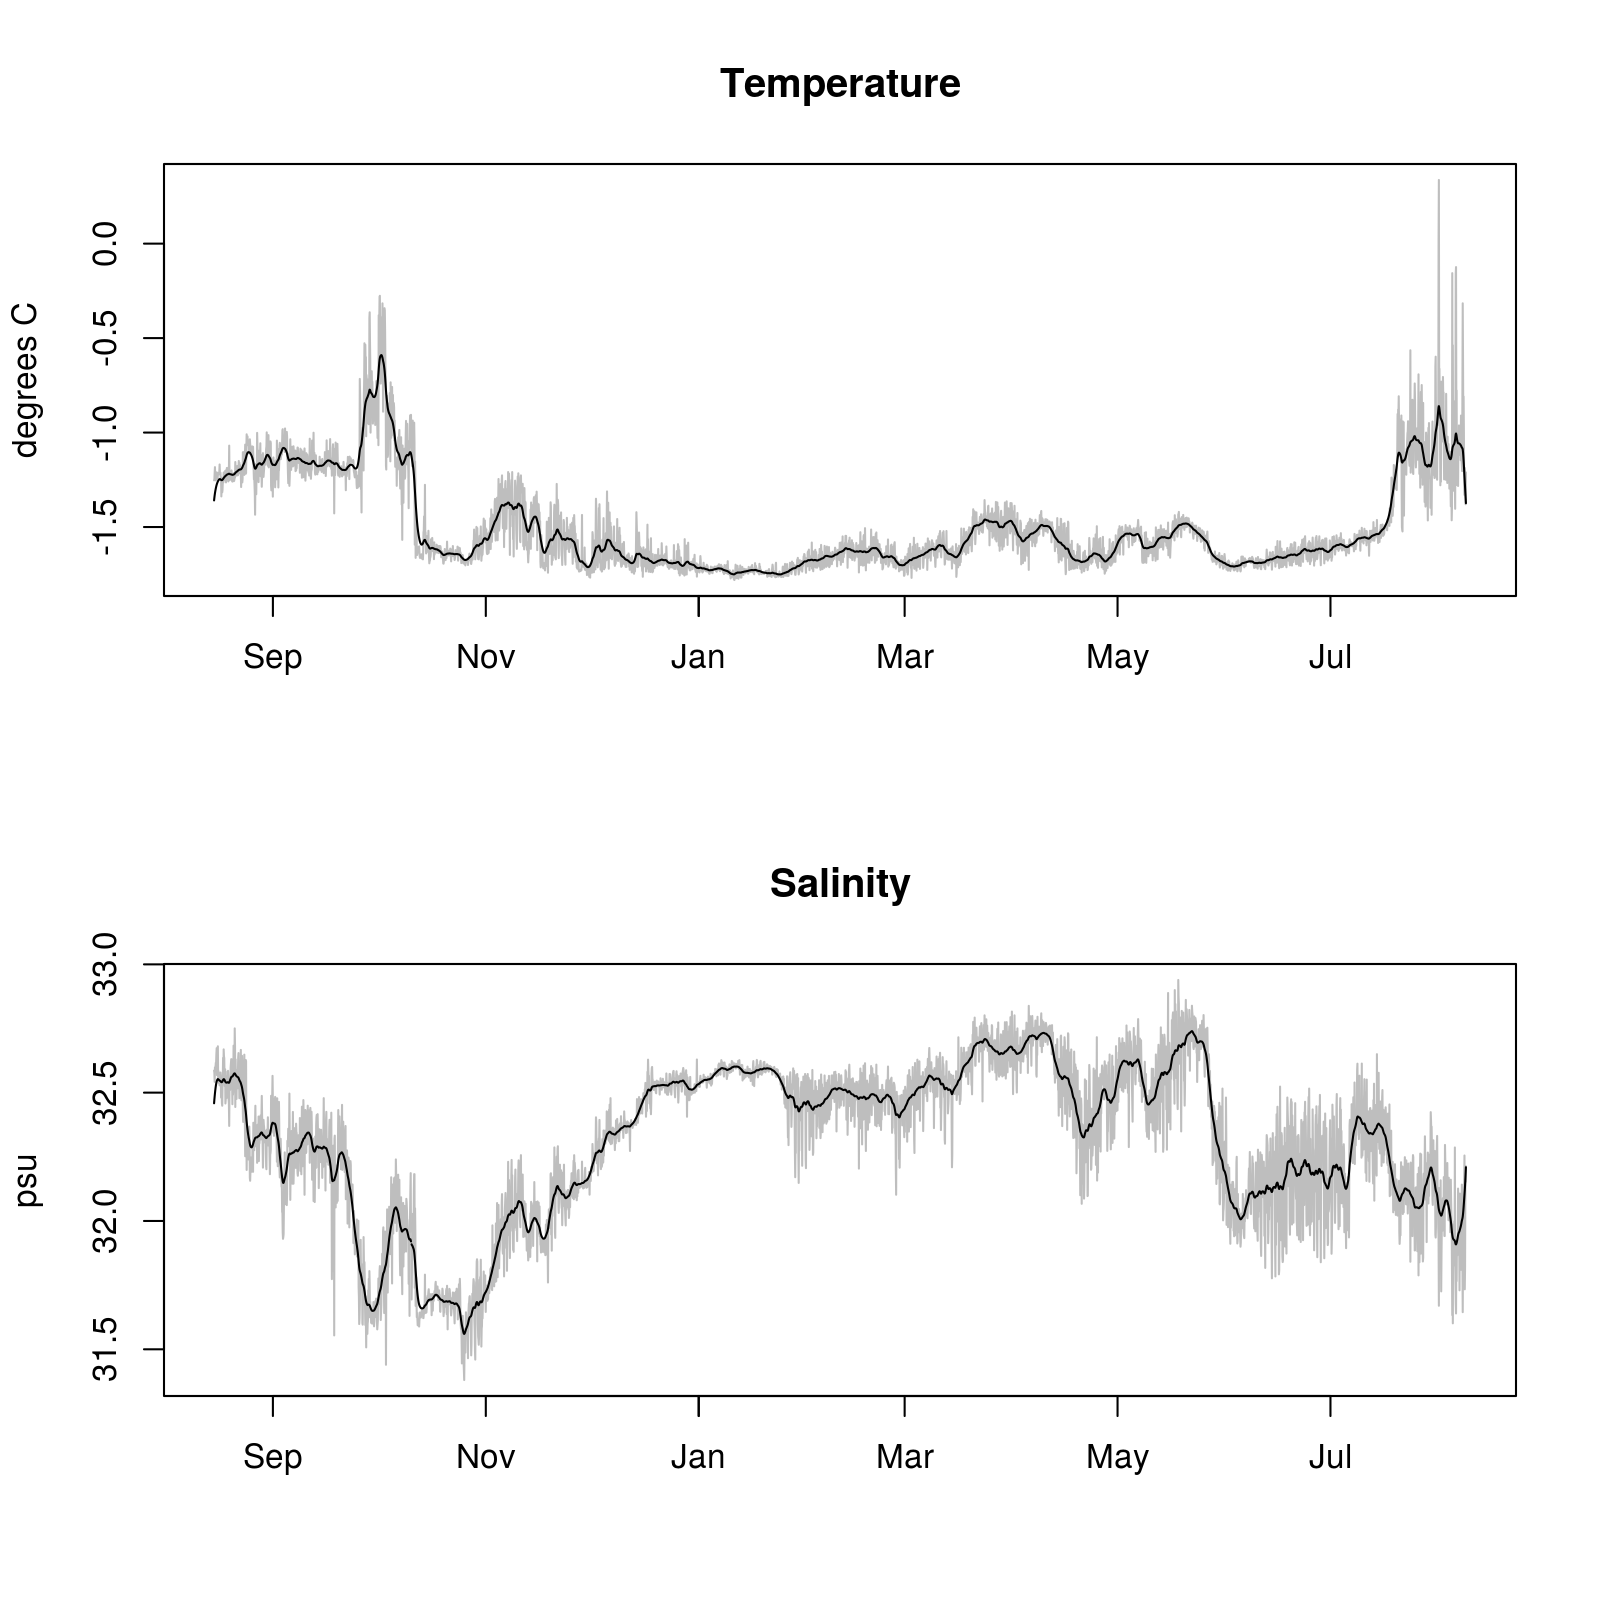
\includegraphics[width = 0.8\textwidth]{./figures/25_lpf_TS_41m_2013_2014.png}
\caption[Low-pass filtered T, S (41 m), 2013-2014]{Low-pass filtered T, S (41 m), August 2013 - August 2014}
\label{f:ctd_41_lpf_2013_2014}
\end{figure}

\begin{figure}  
\centering
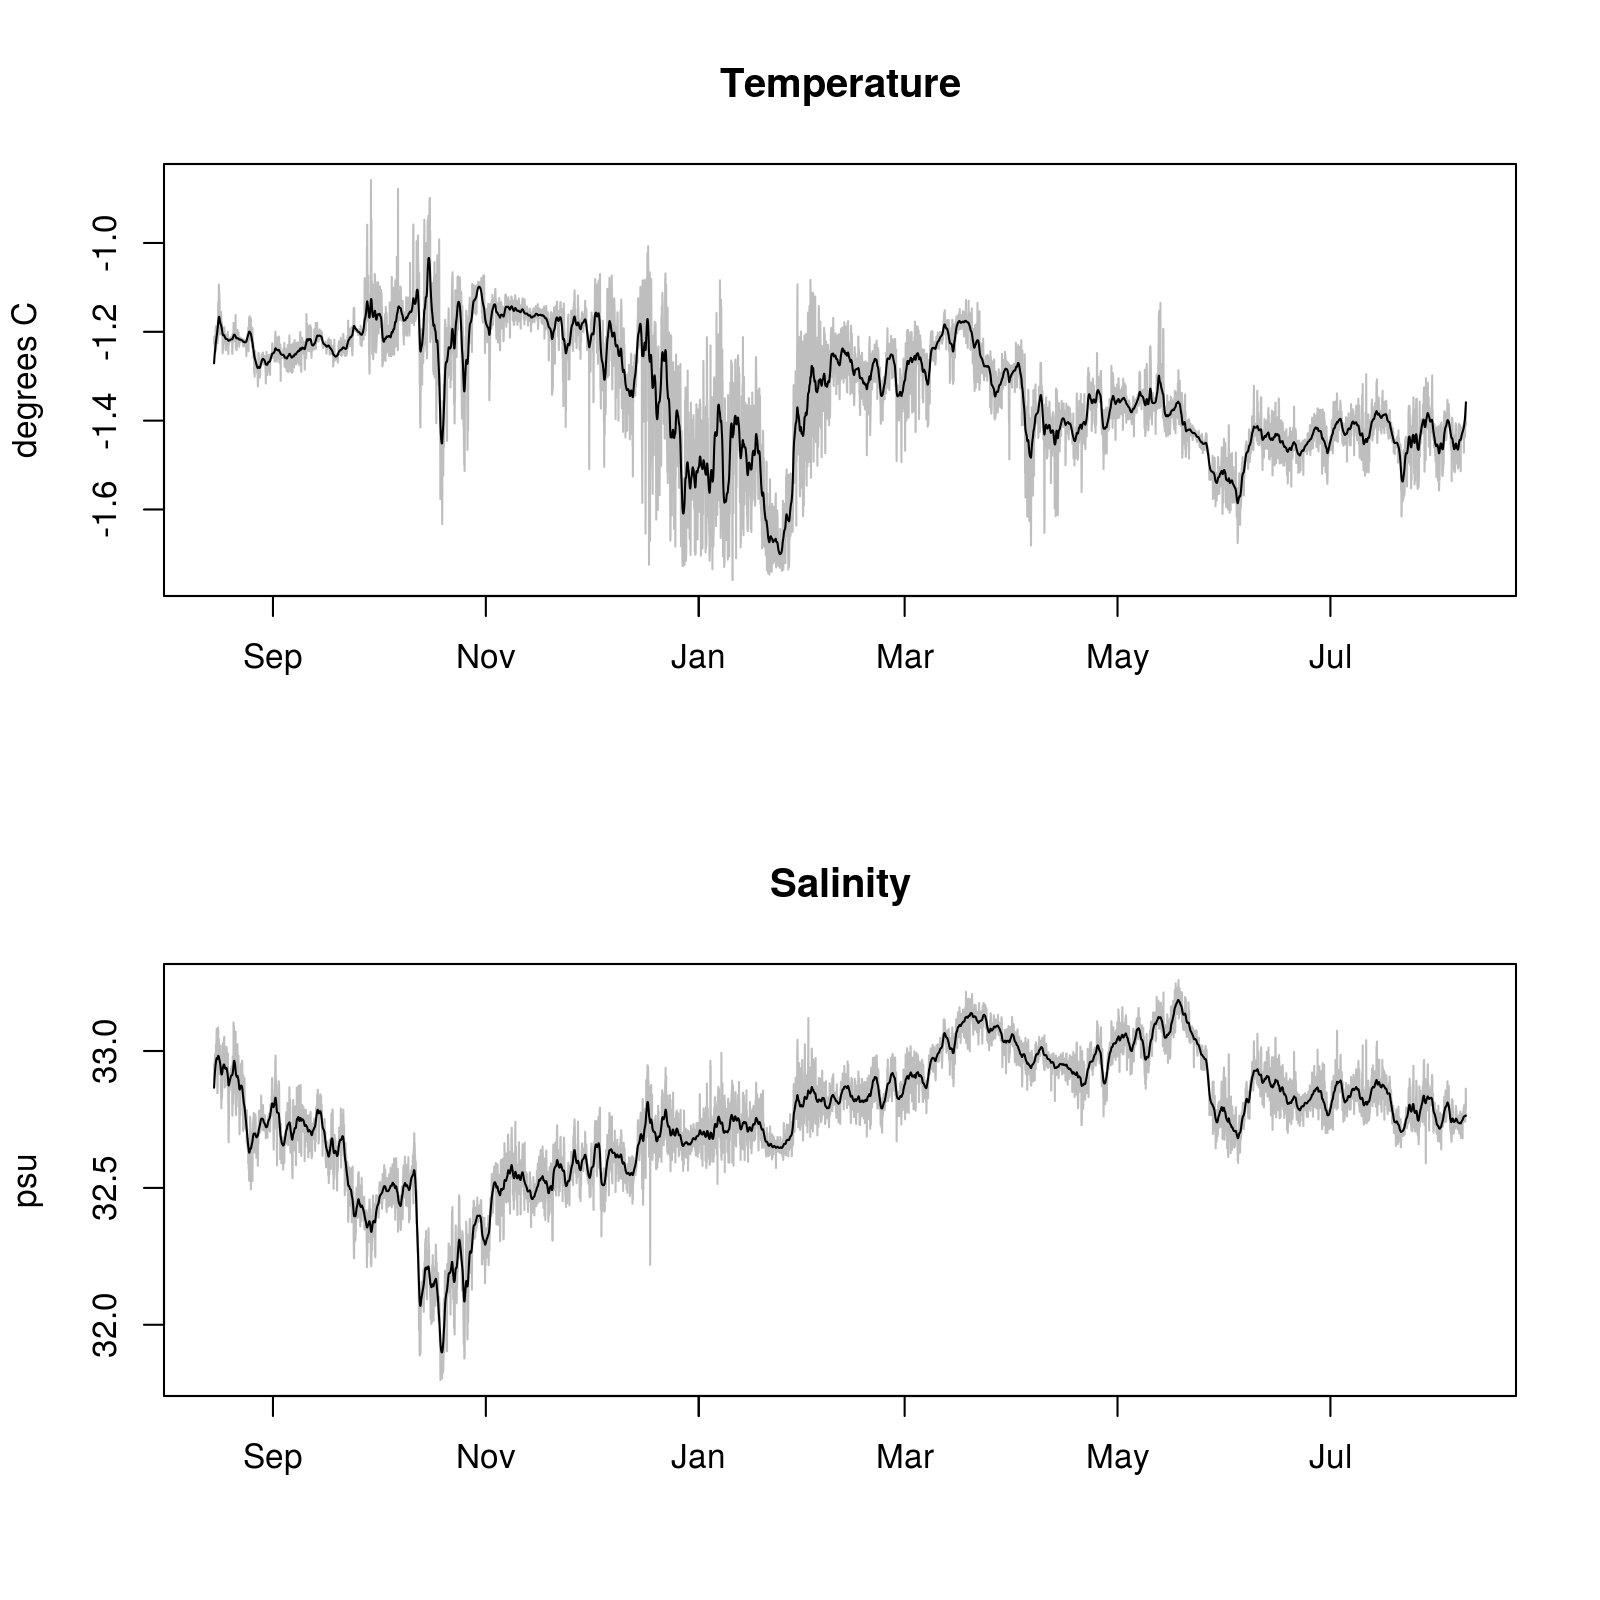
\includegraphics[width = 0.8\textwidth]{./figures/26_lpf_TS_81m_2013_2014.png}
\caption[Low-pass filtered T, S (81 m), 2013-2014]{Low-pass filtered T, S (81 m), August 2013 - August 2014}
\label{f:ctd_81_lpf_2013_2014}
\end{figure}

\begin{figure}  
\centering
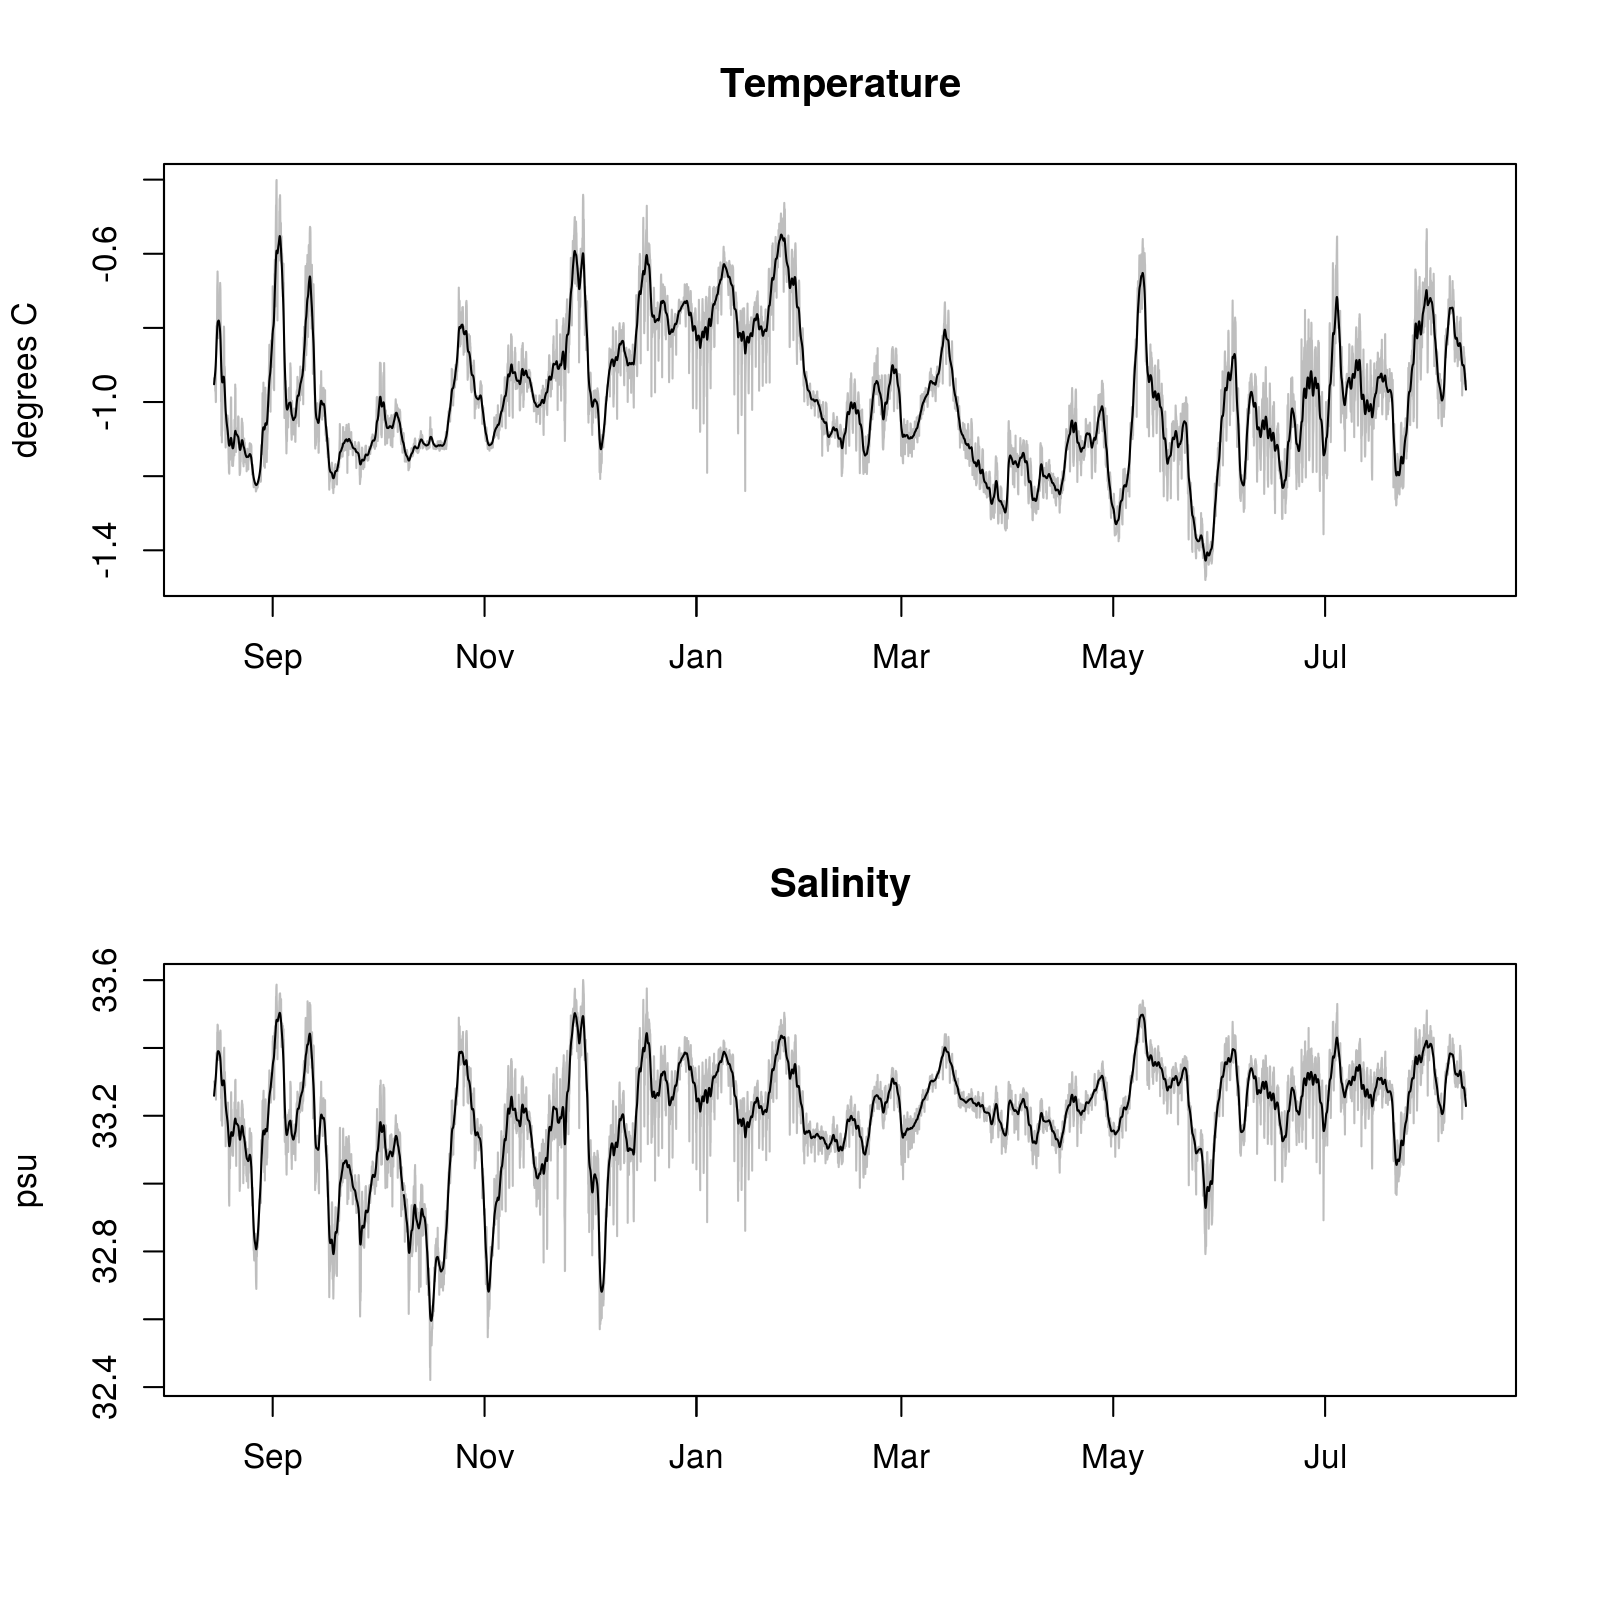
\includegraphics[width = 0.8\textwidth]{./figures/27_lpf_TS_155m_2013_2014.png}
\caption[Low-pass filtered T, S (155 m), 2013-2014]{Low-pass filtered T, S (155 m), August 2013 - August 2014}
\label{f:ctd_155_lpf_2013_2014}
\end{figure}


\begin{figure}  
\centering
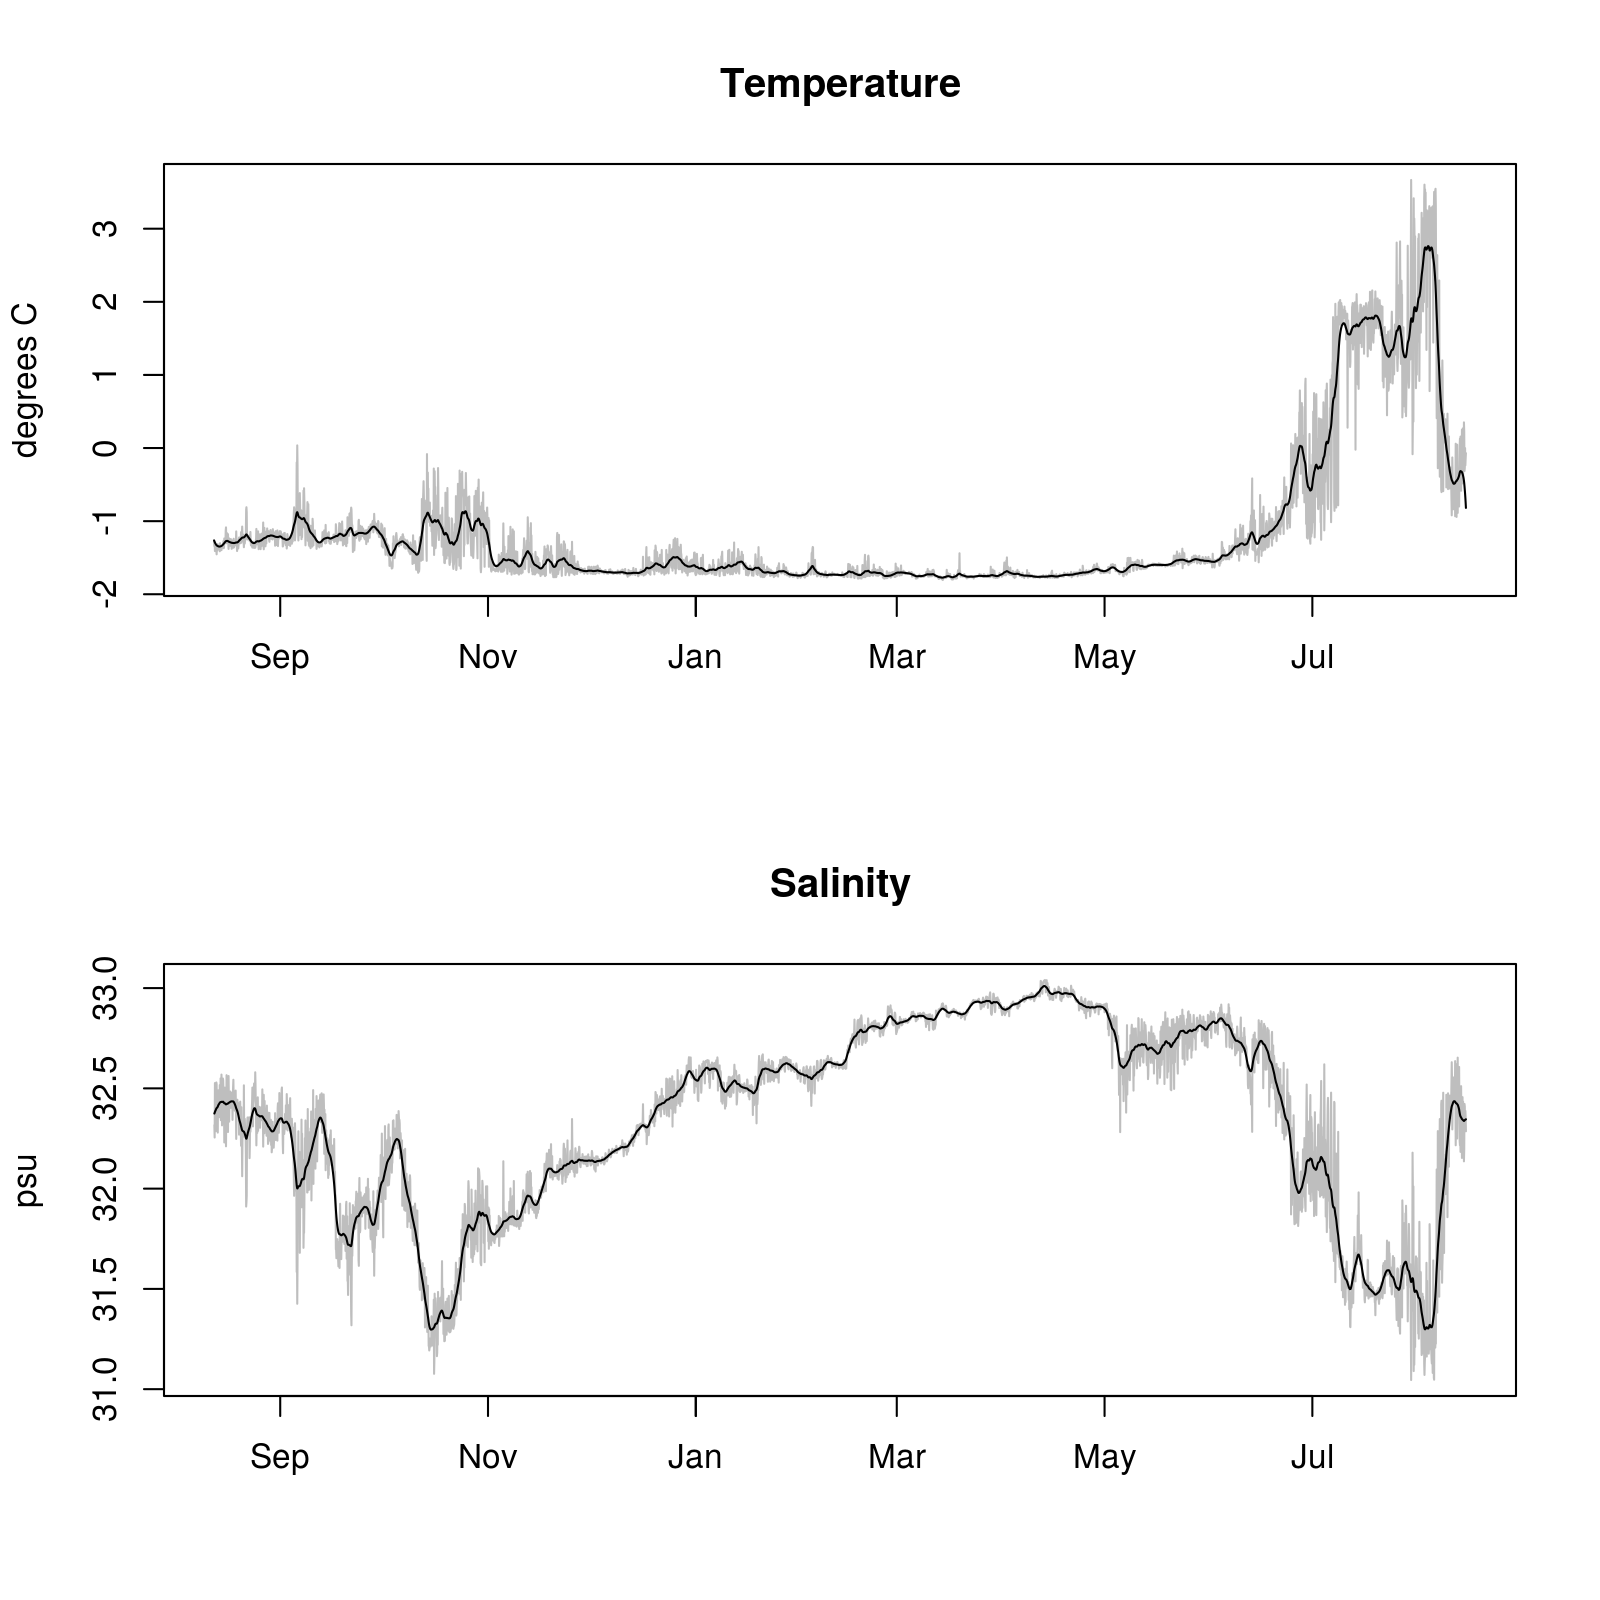
\includegraphics[width = 0.8\textwidth]{./figures/28_lpf_TS_35m_2014_2015.png}
\caption[Low-pass filtered T, S (35 m), 2014-2015]{Low-pass filtered T, S (35 m), August 2014 - August 2015}
\label{f:ctd_35_lpf_2014_2015}
\end{figure}

\begin{figure}  
\centering
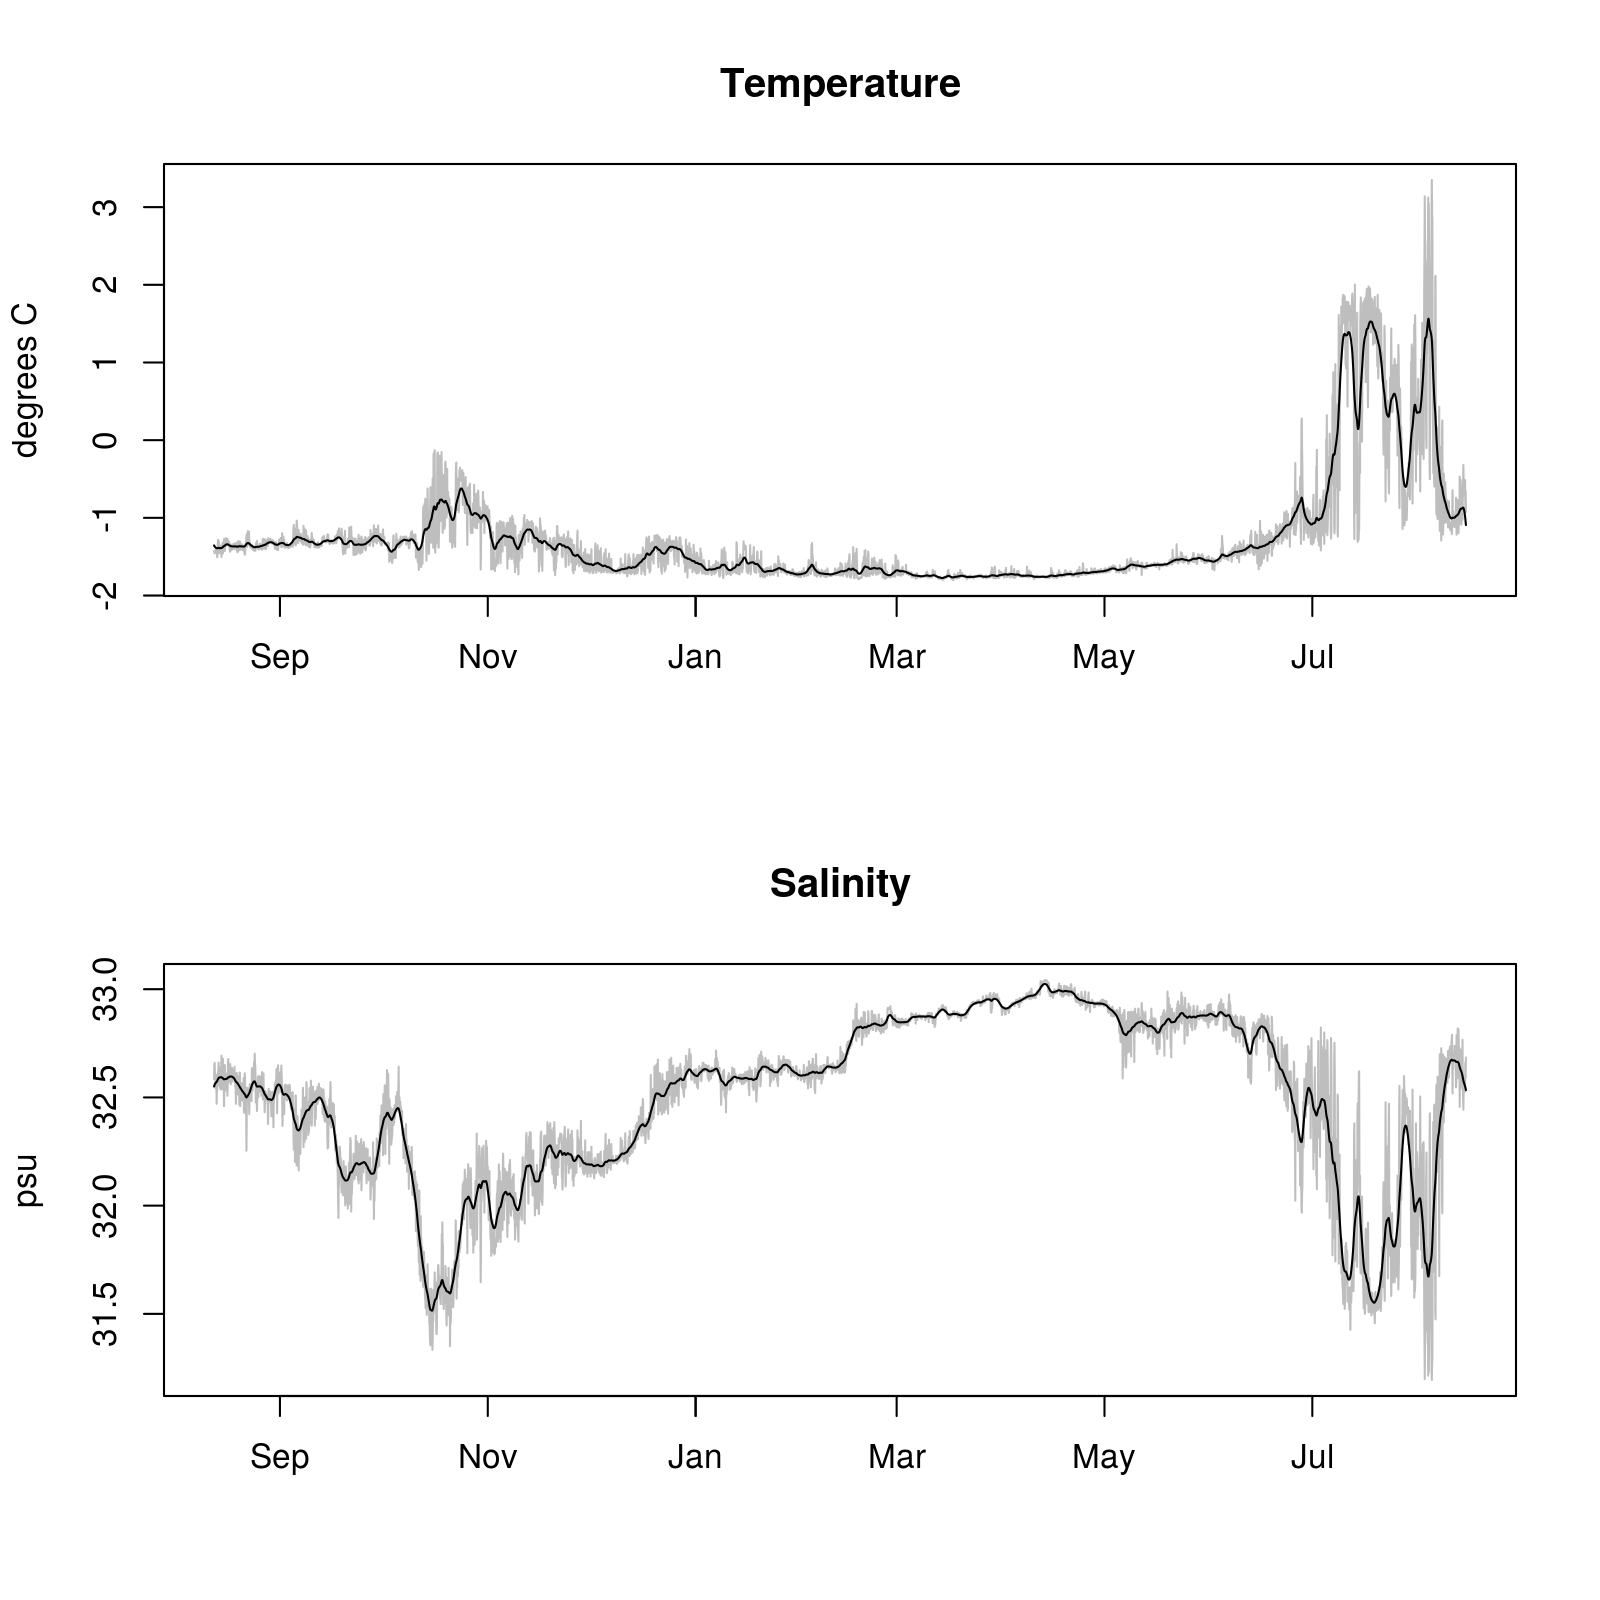
\includegraphics[width = 0.8\textwidth]{./figures/29_lpf_TS_47m_2014_2015.png}
\caption[Low-pass filtered T, S (47 m), 2014-2015]{Low-pass filtered T, S (47 m), August 2014 - August 2015}
\label{f:ctd_47_lpf_2014_2015}
\end{figure}

\begin{figure}  
\centering
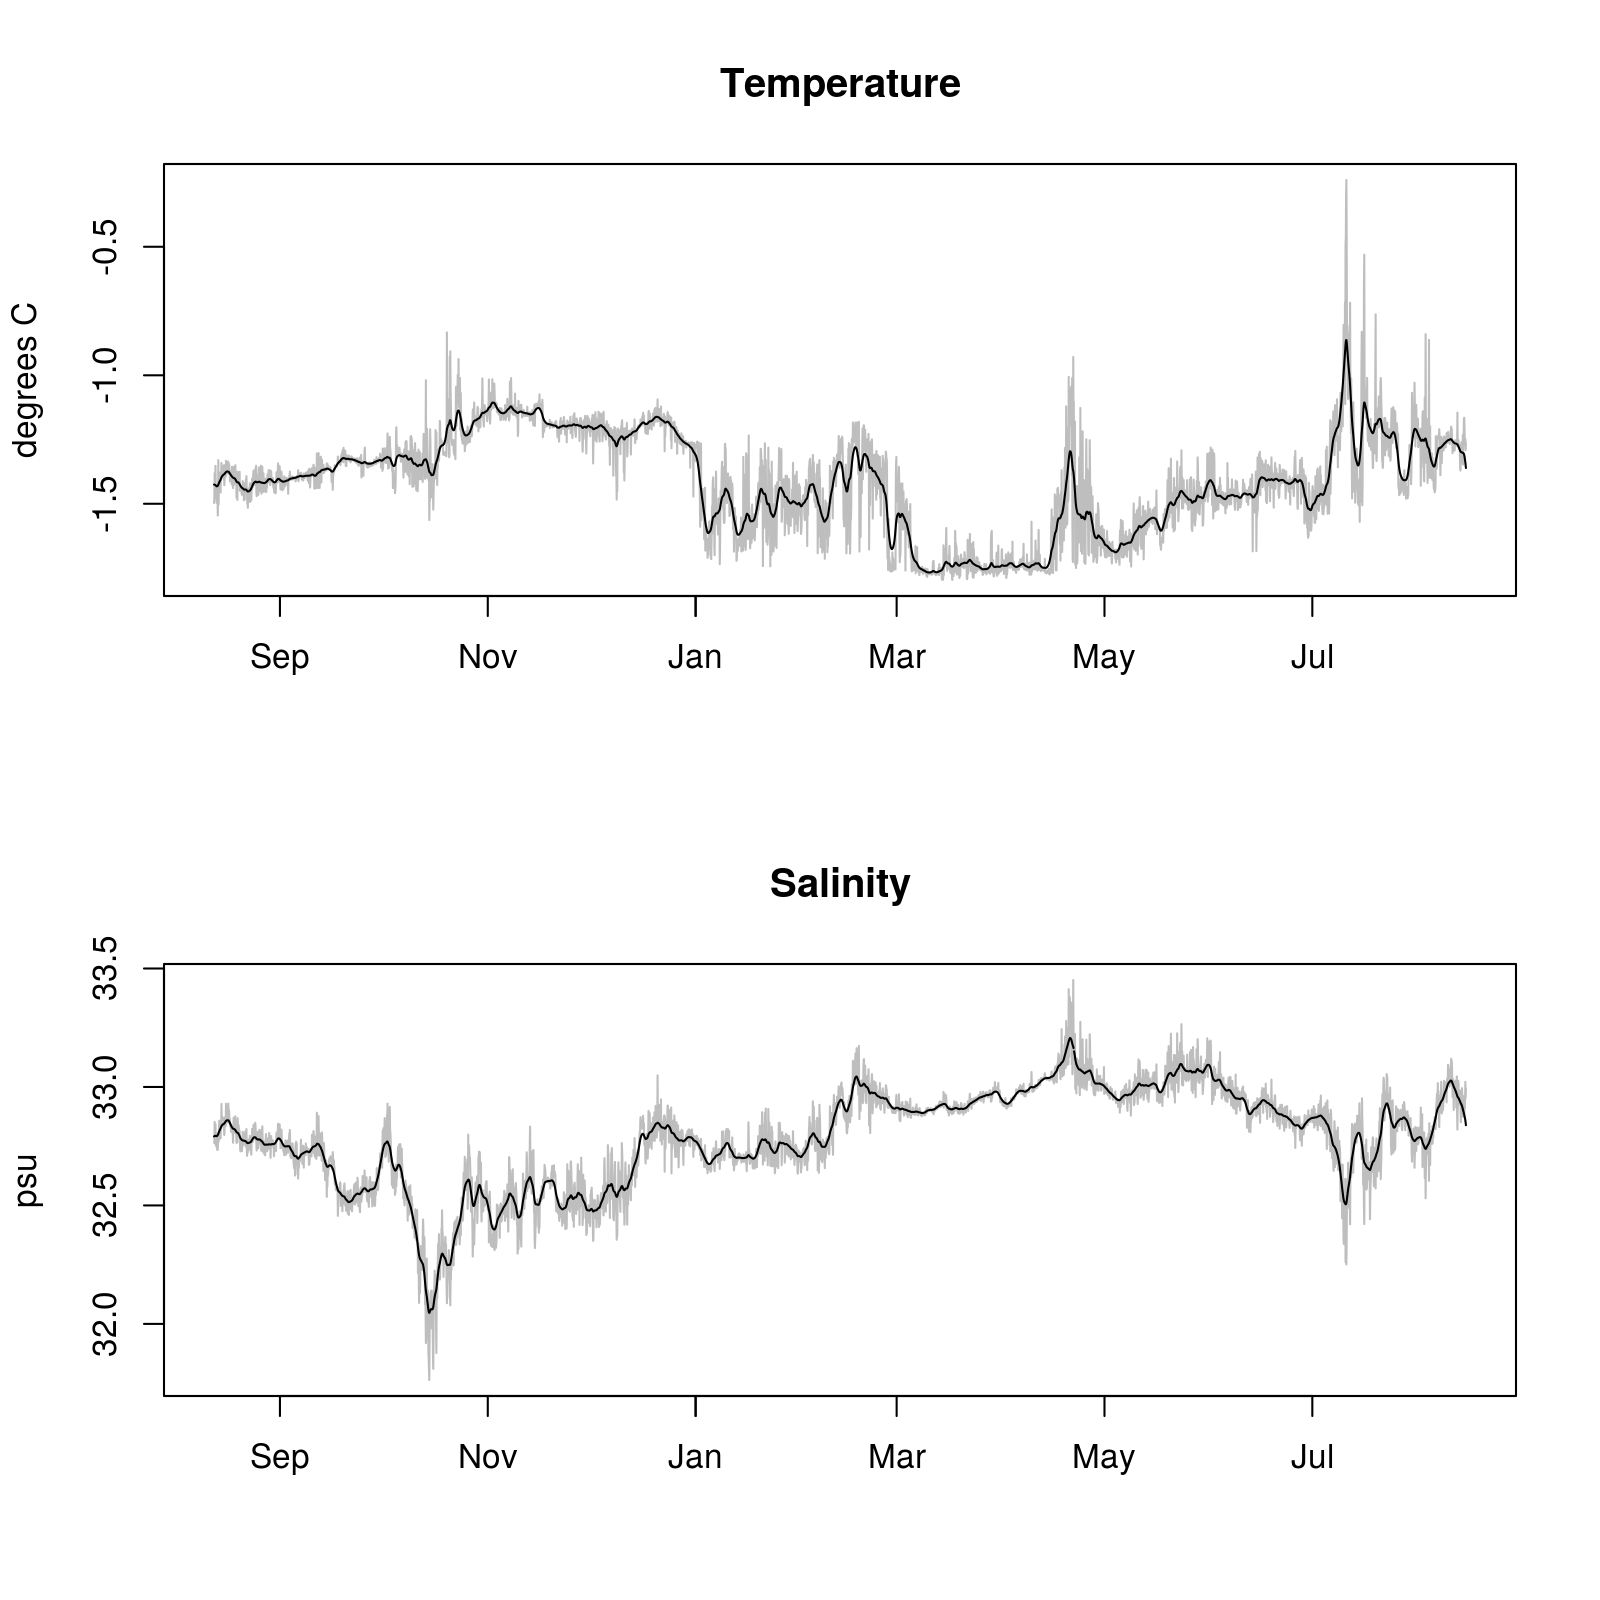
\includegraphics[width = 0.8\textwidth]{./figures/30_lpf_TS_81m_2014_2015.png}
\caption[Low-pass filtered T, S (81 m), 2014-2015]{Low-pass filtered T, S (81 m), August 2014 - August 2015}
\label{f:ctd_81_lpf_2014_2015}
\end{figure}

\begin{figure}  
\centering
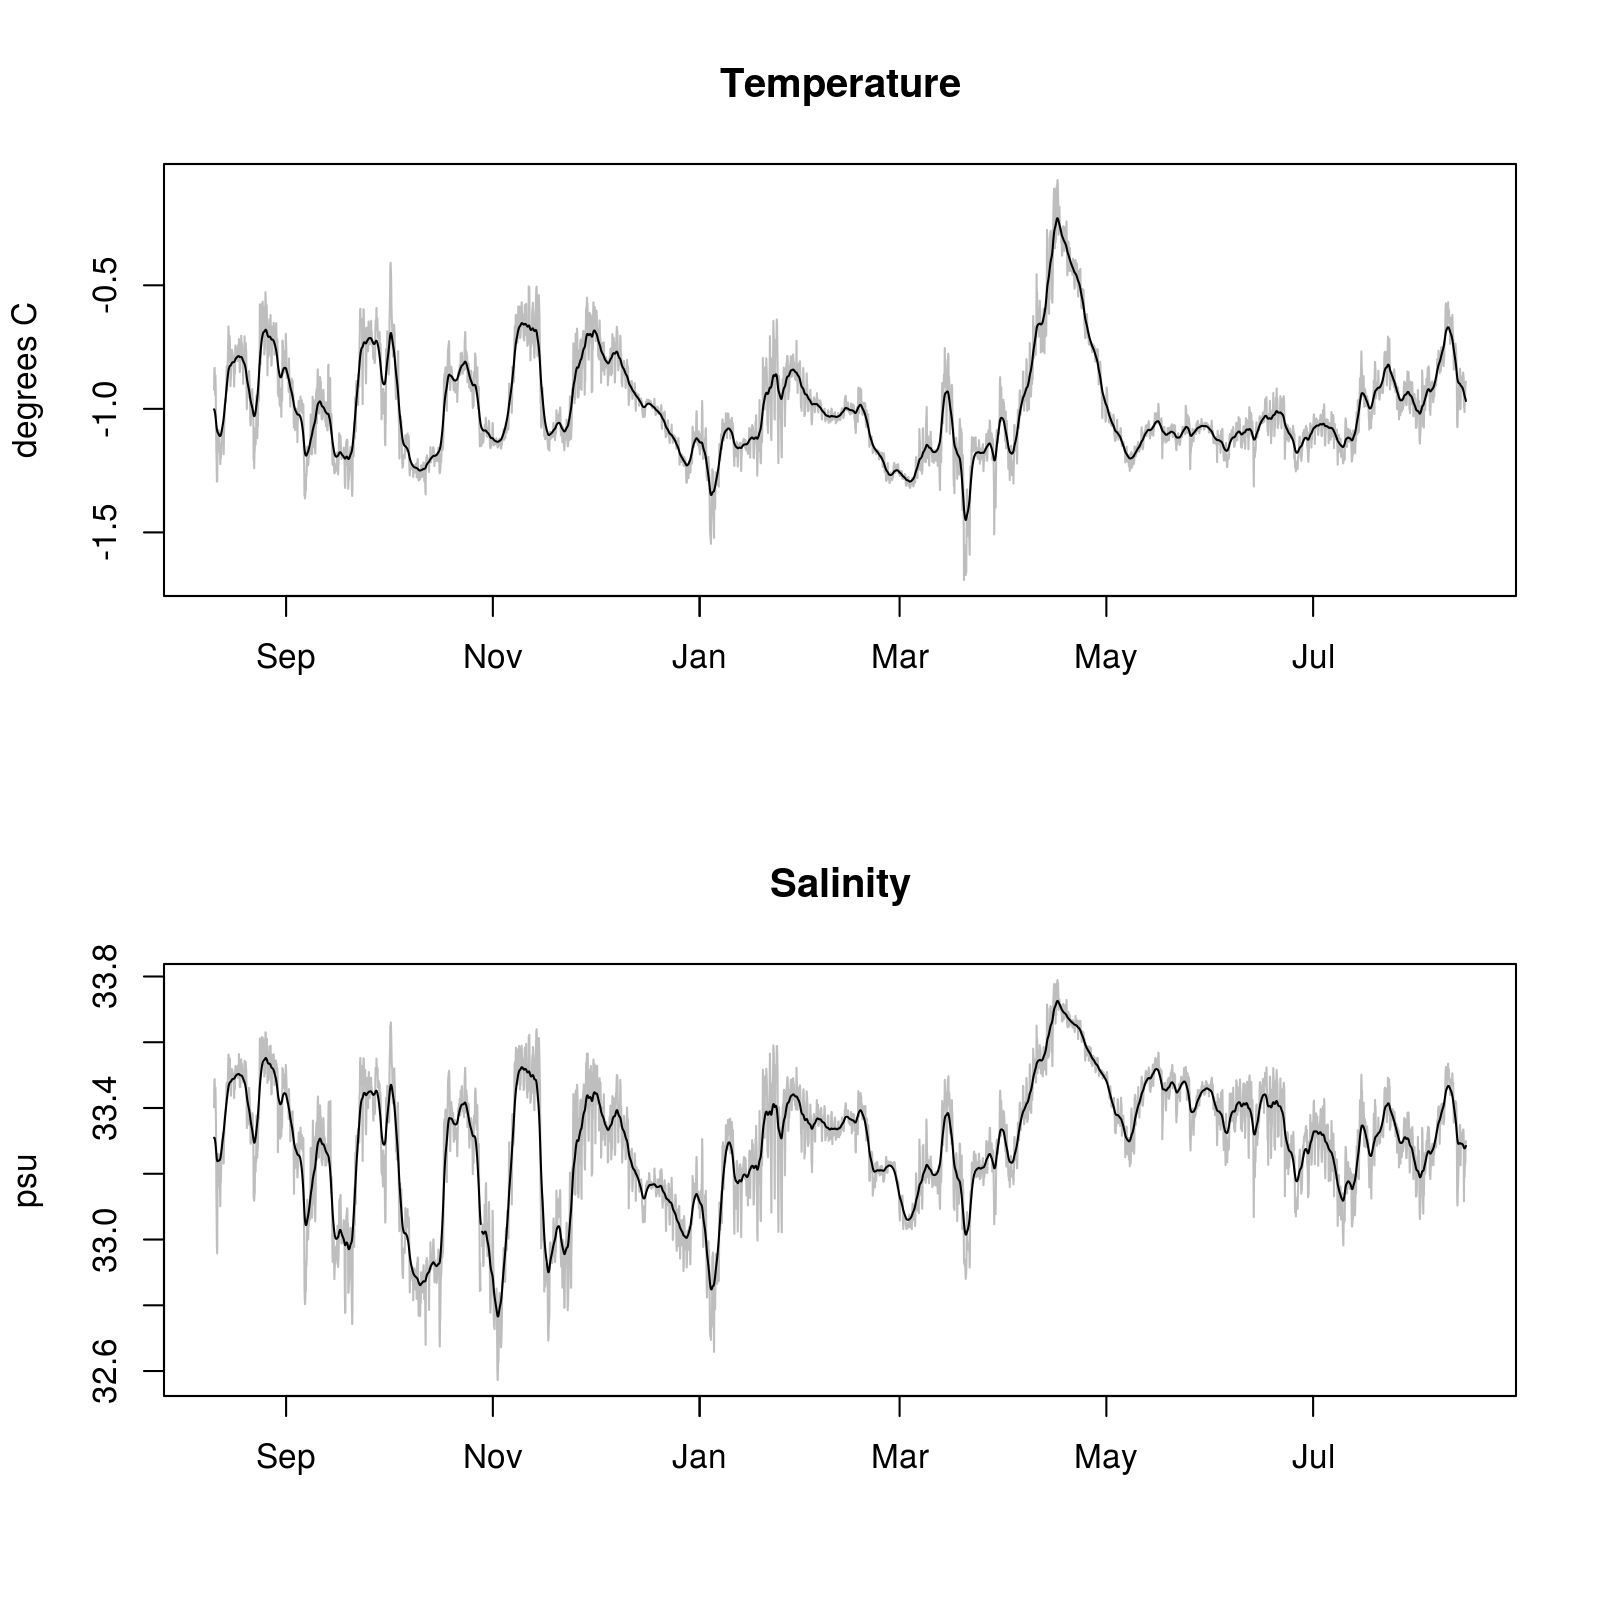
\includegraphics[width = 0.8\textwidth]{./figures/31_lpf_TS_155m_2014_2015.png}
\caption[Low-pass filtered T, S (155 m), 2014-2015]{Low-pass filtered T, S (155 m), August 2014 - August 2015}
\label{f:ctd_155_lpf_2014_2015}
\end{figure}


\begin{figure}  
\centering
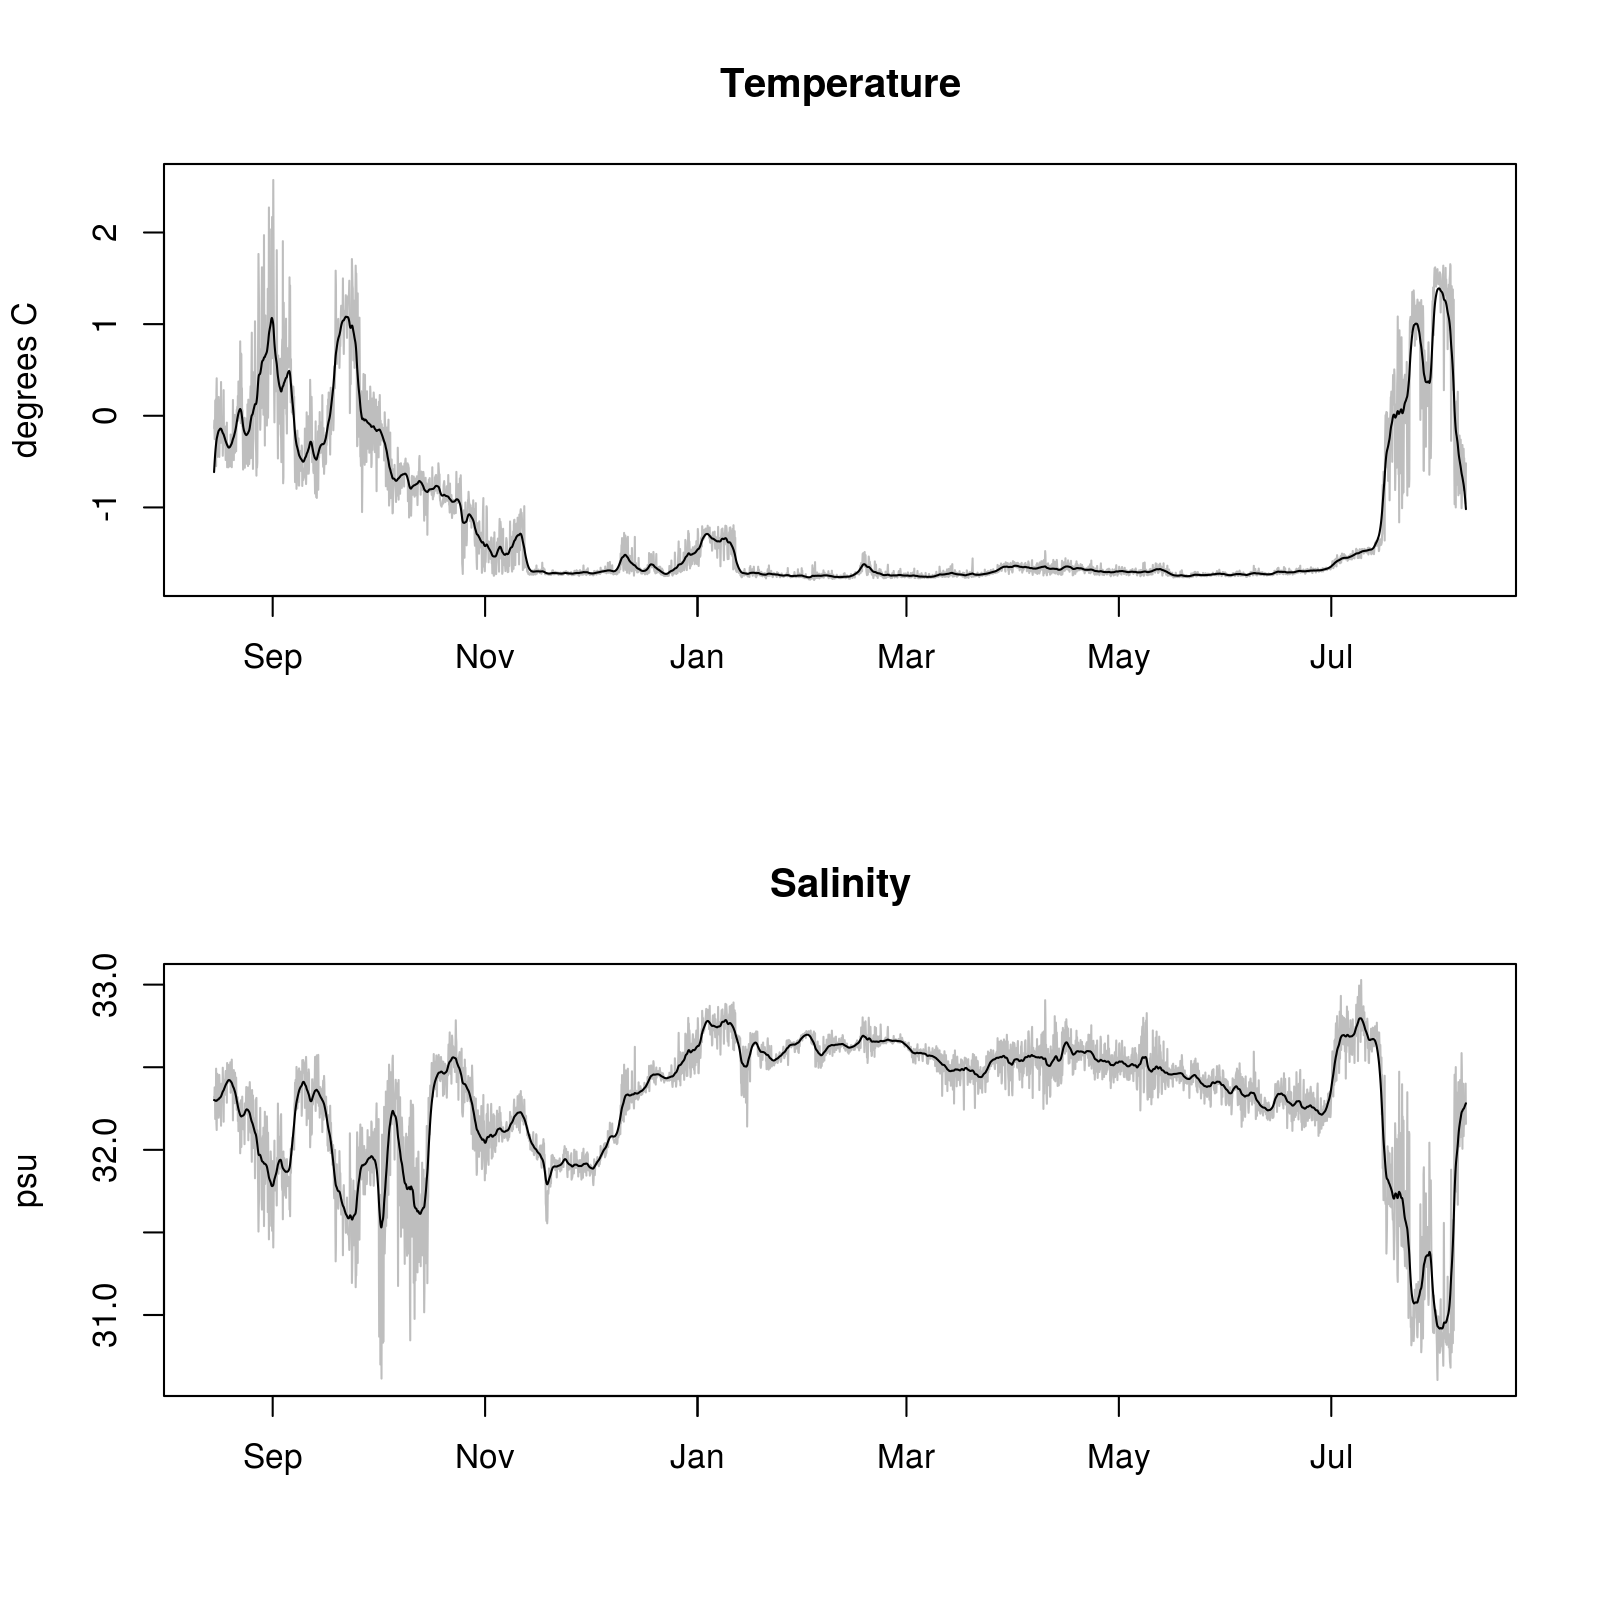
\includegraphics[width = 0.8\textwidth]{./figures/32_lpf_TS_35m_2015_2016.png}
\caption[Low-pass filtered T, S (35 m), 2015-2016]{Low-pass filtered T, S (35 m), August 2015 - August 2016}
\label{f:ctd_35_lpf_2015_2016}
\end{figure}

\begin{figure}  
\centering
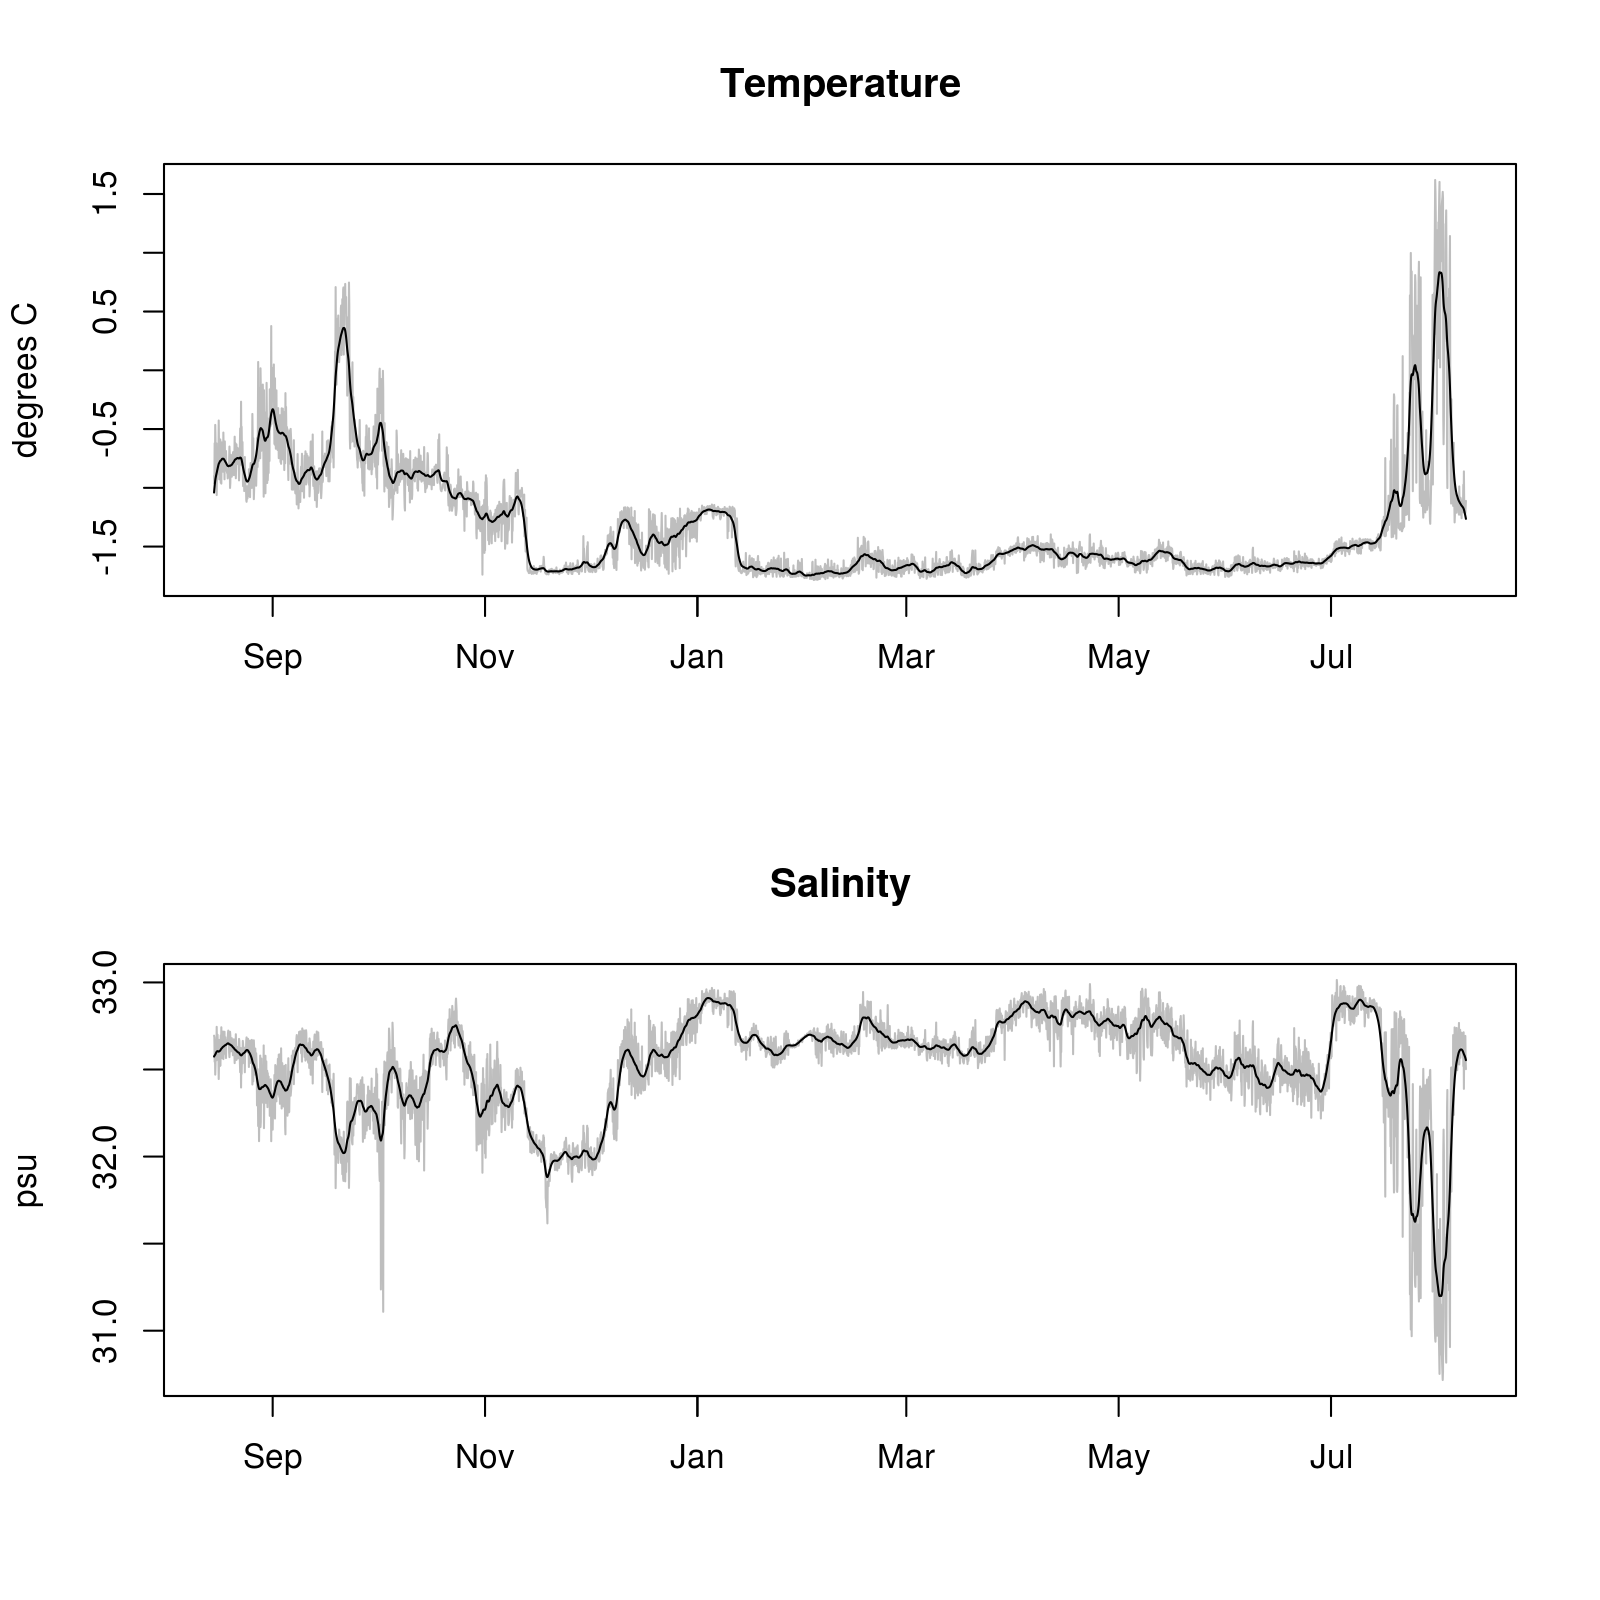
\includegraphics[width = 0.8\textwidth]{./figures/33_lpf_TS_47m_2015_2016.png}
\caption[Low-pass filtered T, S (47 m), 2015-2016]{Low-pass filtered T, S (47 m), August 2015 - August 2016}
\label{f:ctd_47_lpf_2015_2016}
\end{figure}

\begin{figure}  
\centering
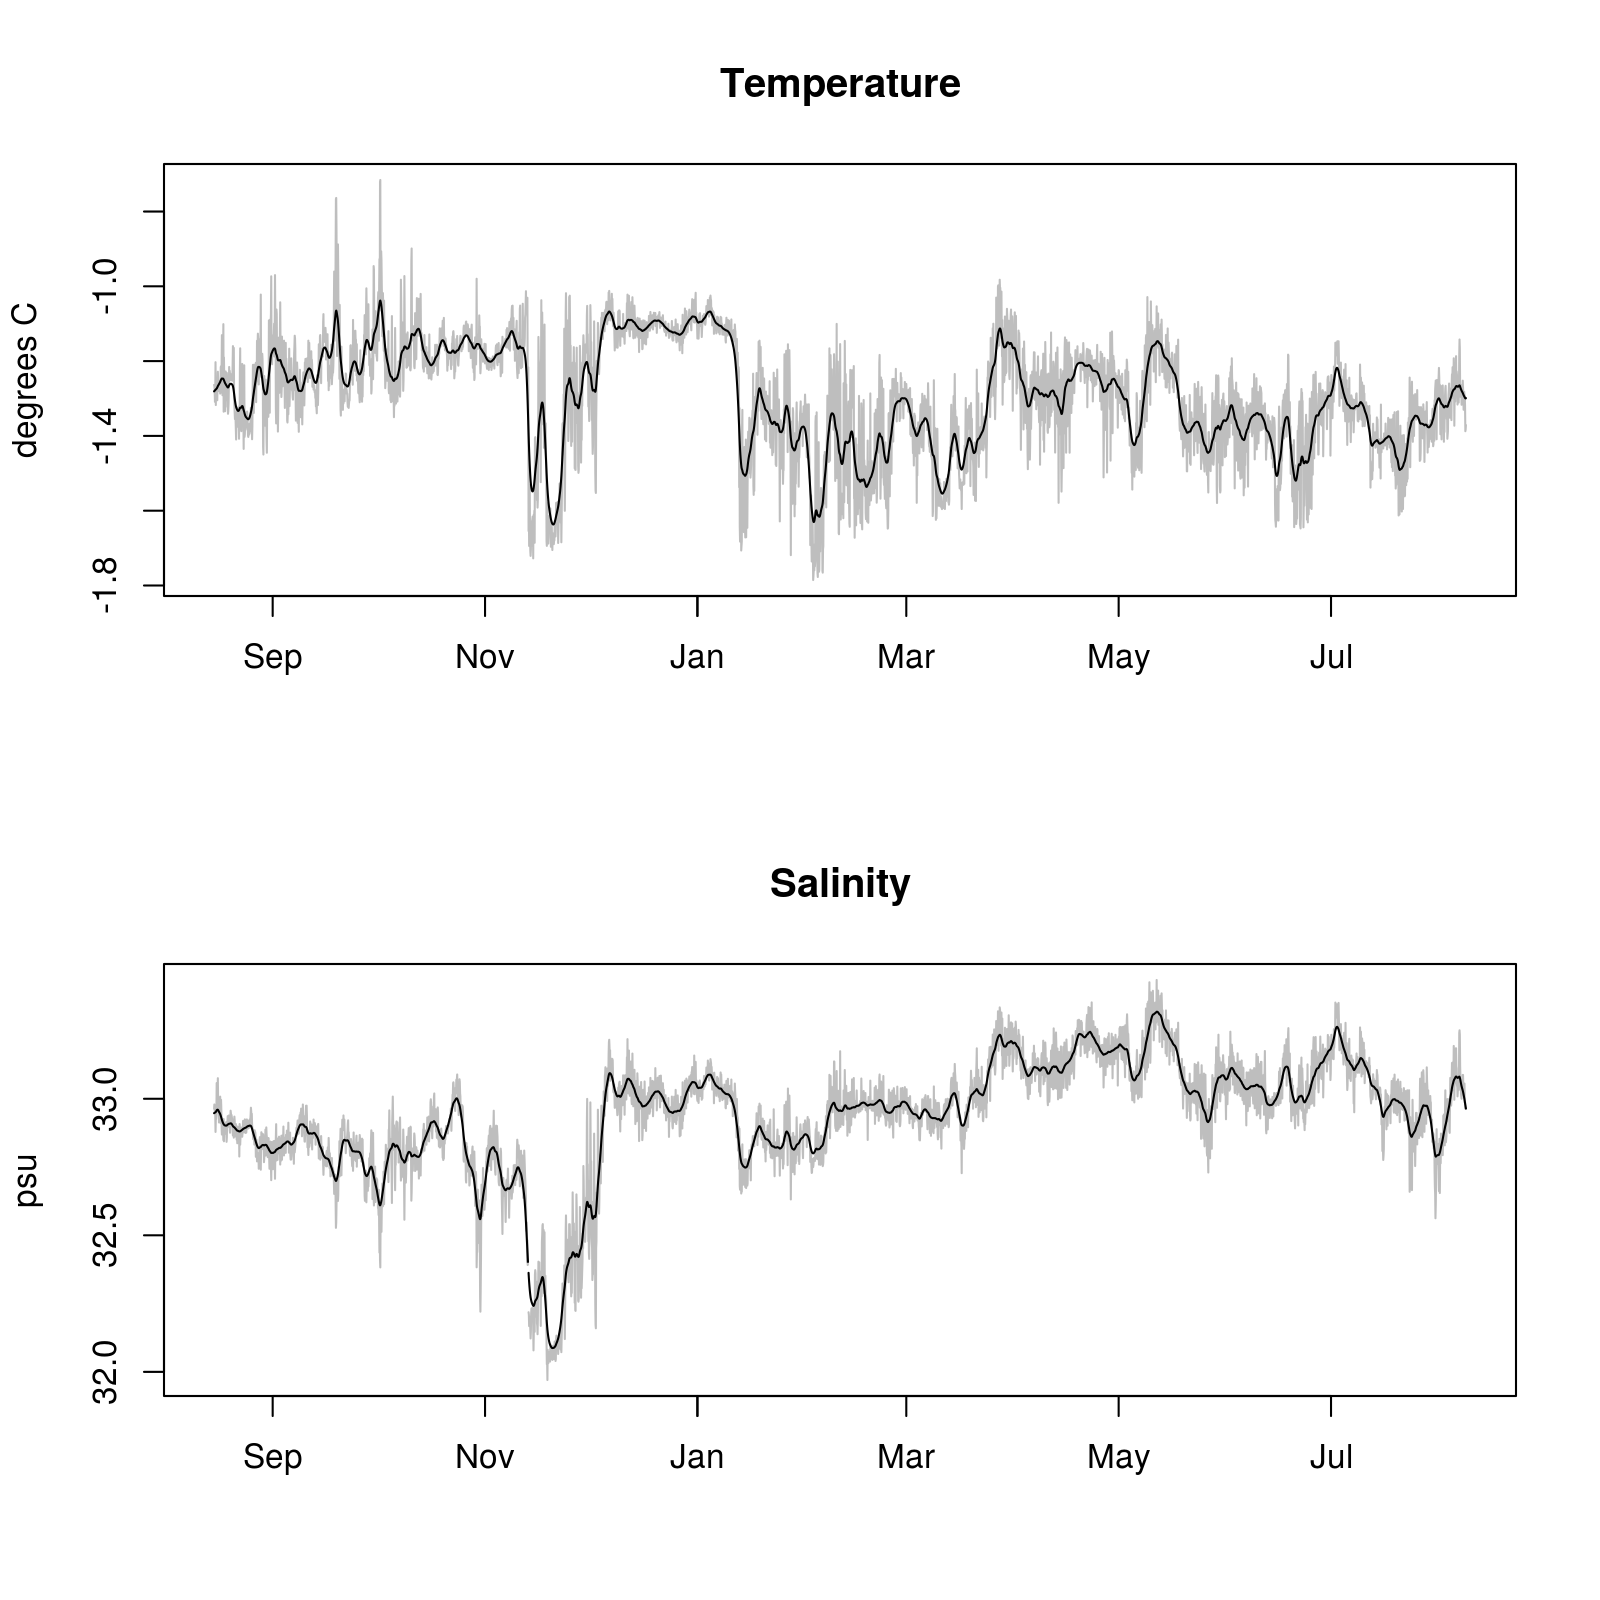
\includegraphics[width = 0.8\textwidth]{./figures/34_lpf_TS_81m_2015_2016.png}
\caption[Low-pass filtered T, S (81 m), 2015-2016]{Low-pass filtered T, S (81 m), August 2015 - August 2016}
\label{f:ctd_81_lpf_2015_2016}
\end{figure}

\begin{figure}  
\centering
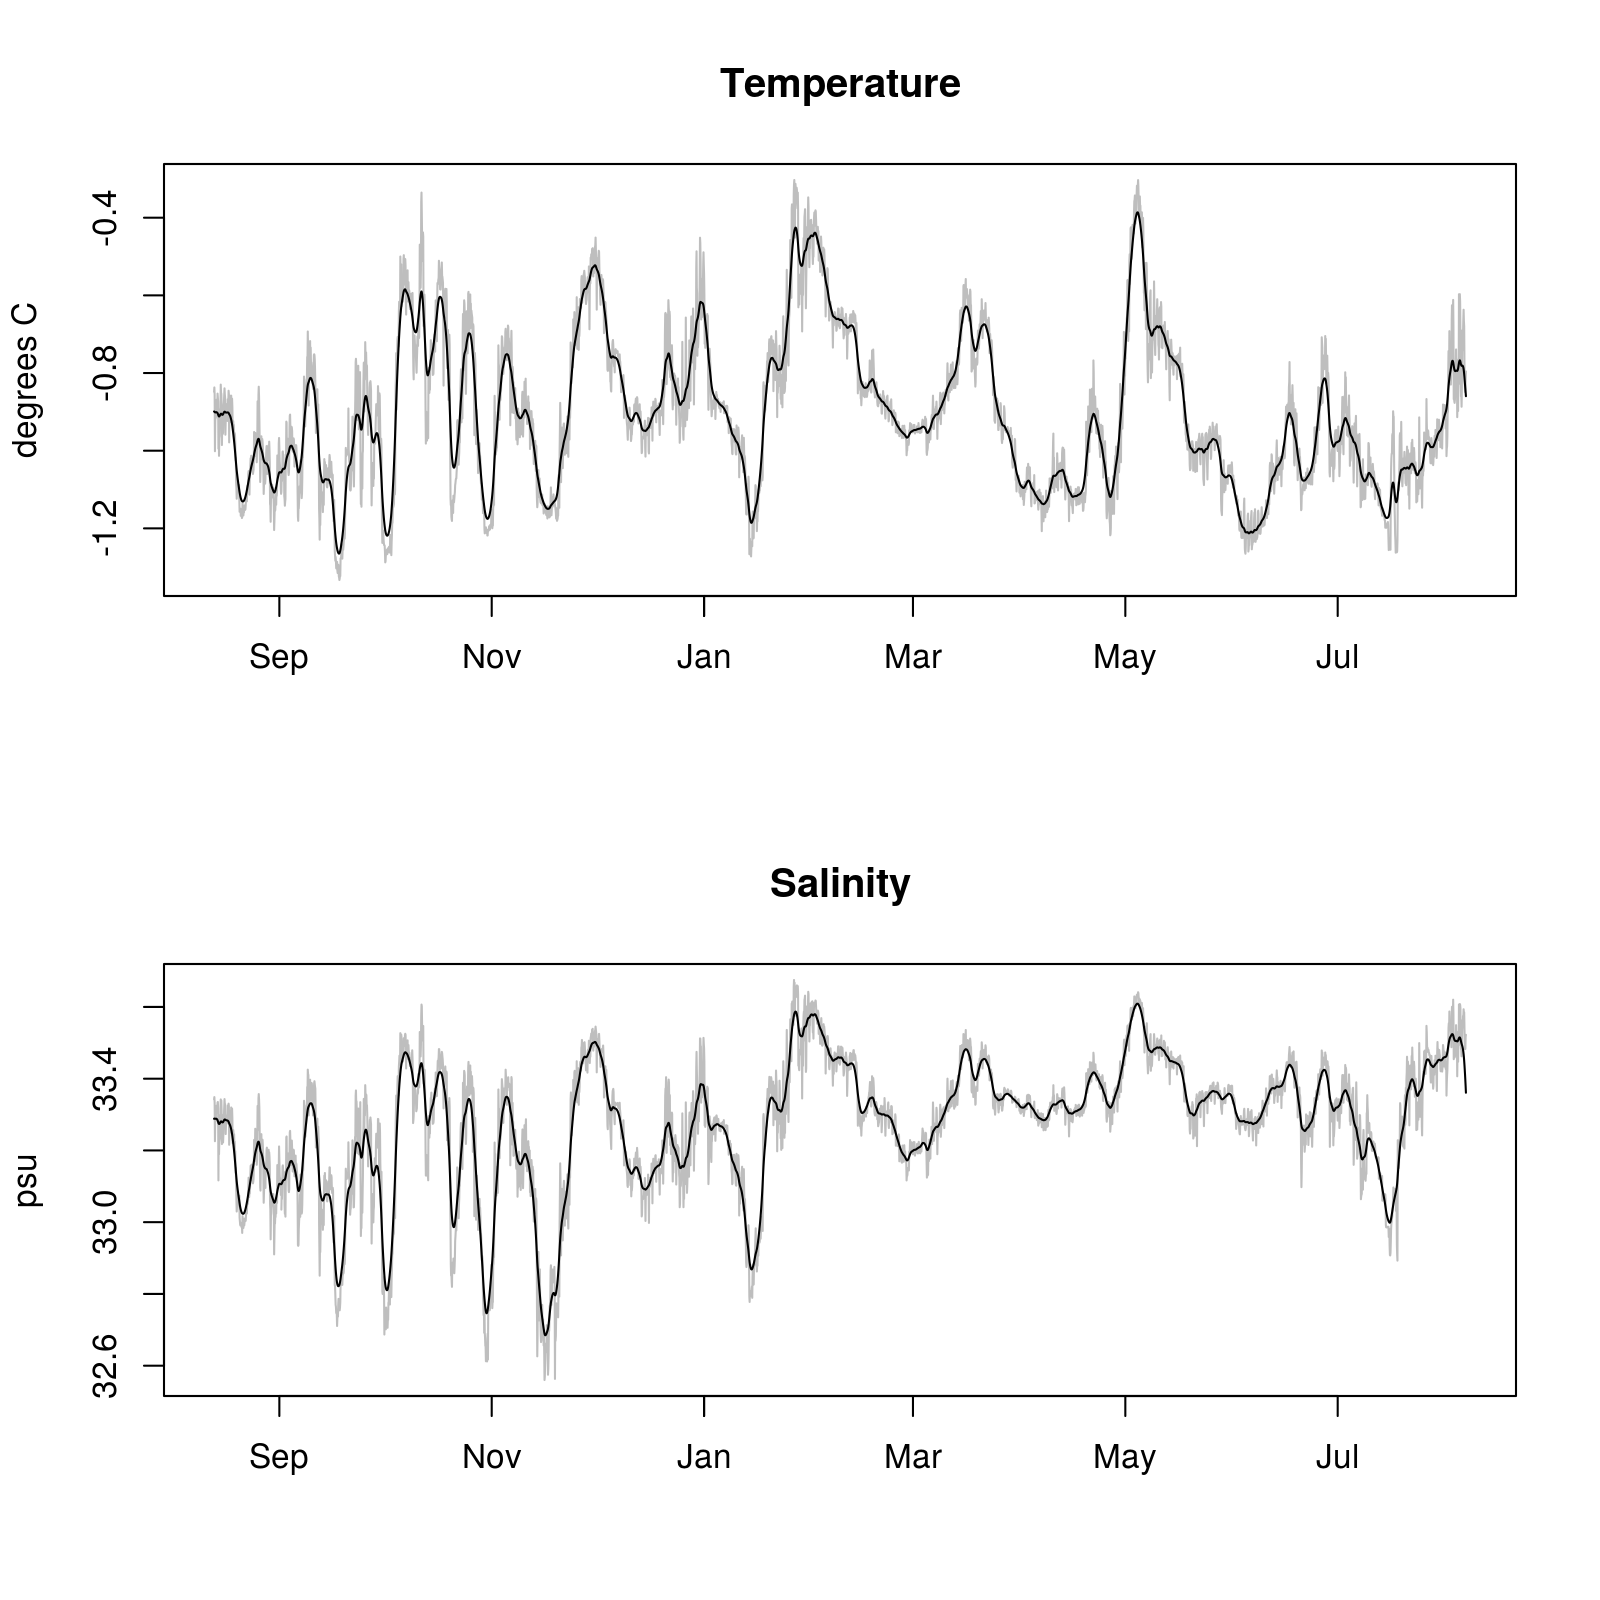
\includegraphics[width = 0.8\textwidth]{./figures/35_lpf_TS_155m_2015_2016.png}
\caption[Low-pass filtered T, S (155 m), 2015-2016]{Low-pass filtered T, S (155 m), August 2015 - August 2016}
\label{f:ctd_155_lpf_2015_2016}
\end{figure}




\begin{figure}
\centering
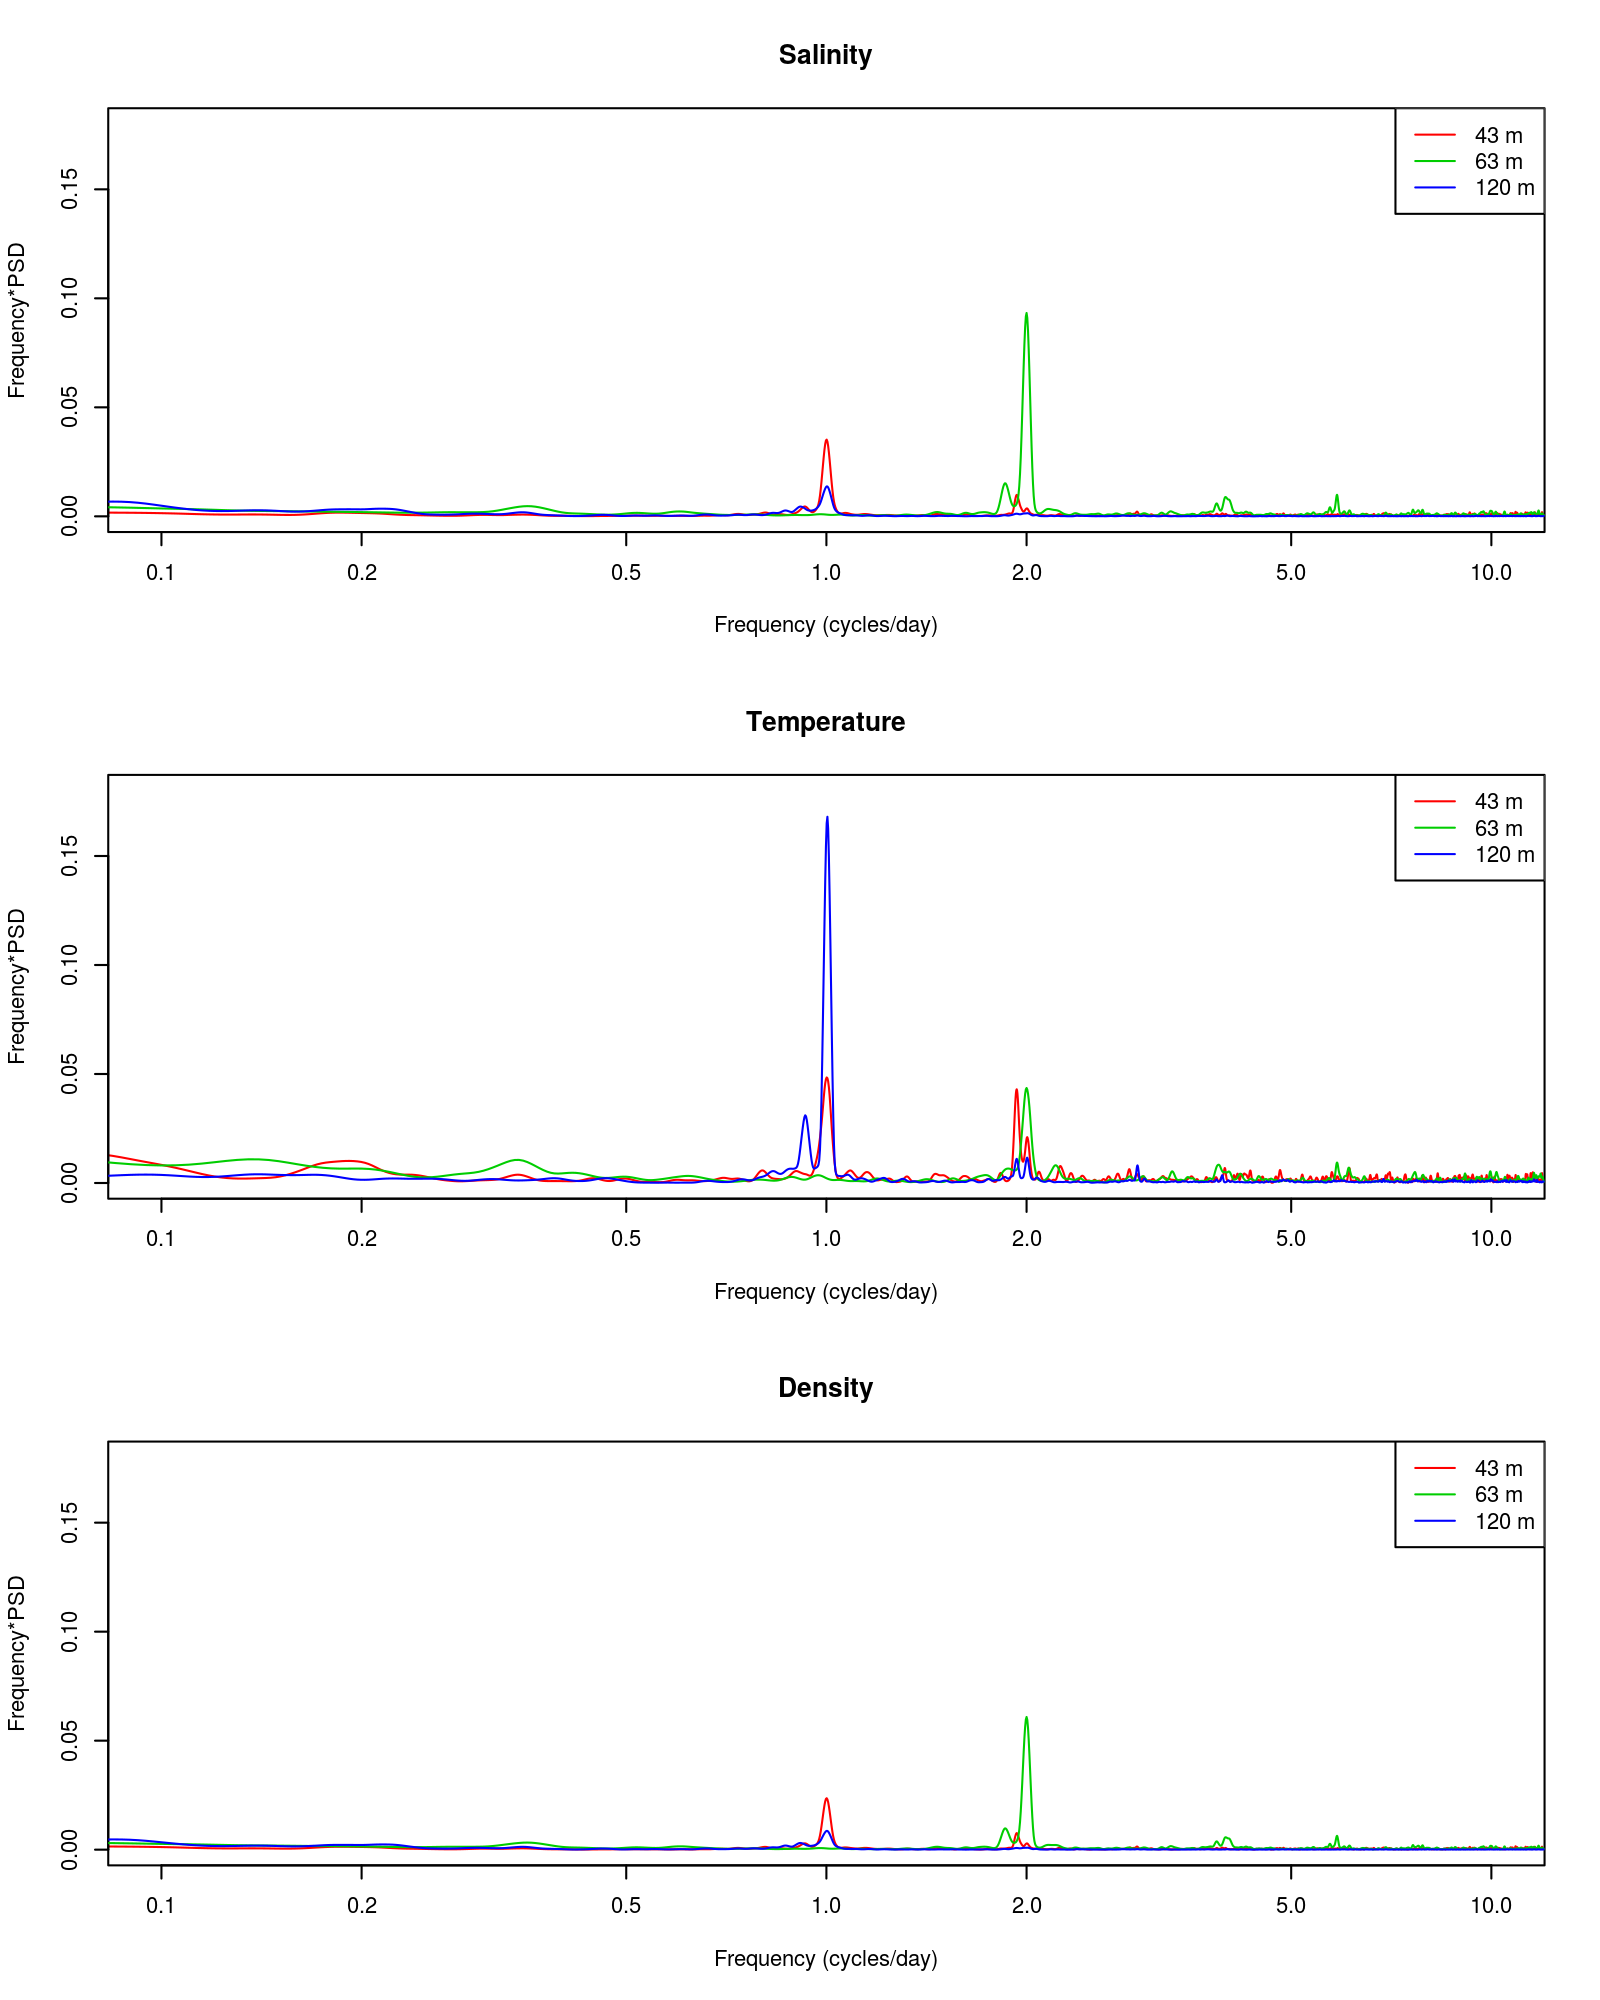
\includegraphics[width = 0.8\textwidth]{./figures/10_mctd_ps_2011_2012.png}
\caption[Power spectra of moored CTD, 2011-2012]{Power spectra of moored CTD data, August 2011 - August 2012.}
\label{f:mctd_ps_2011_2012}
\end{figure}

\begin{figure}
\centering
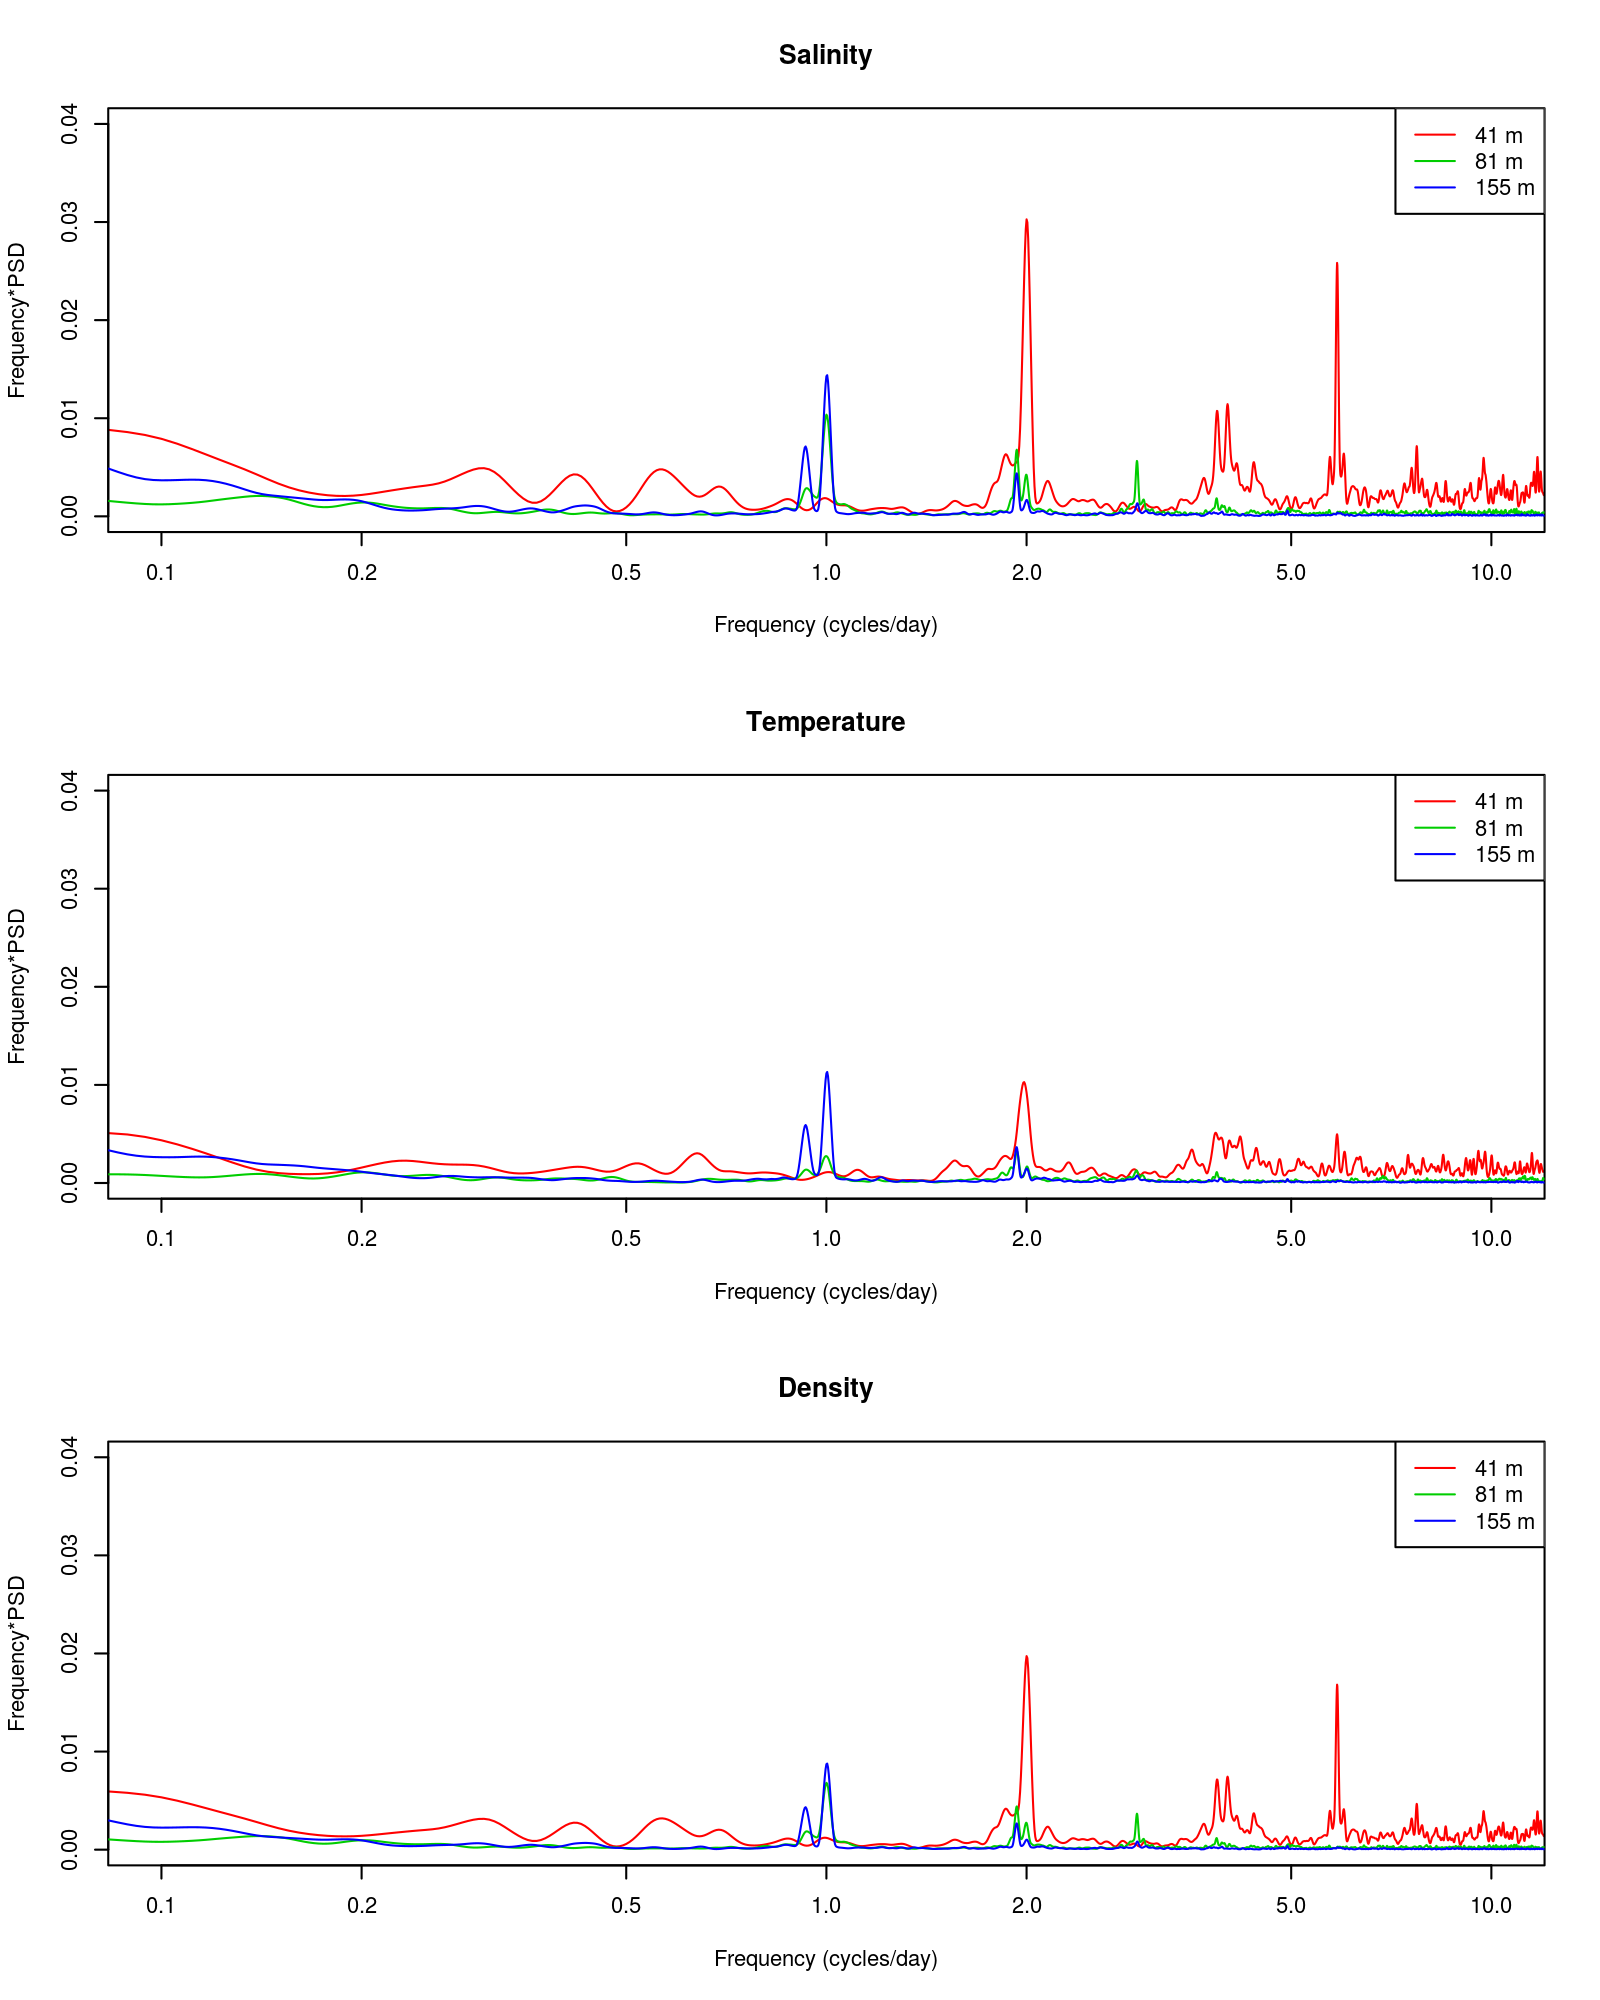
\includegraphics[width = 0.8\textwidth]{./figures/11_mctd_ps_2012_2013.png}
\caption[Power spectra of moored CTD, 2012-2013]{Power spectra of moored CTD data, August 2012 - August 2013.}
\label{f:mctd_ps_2012_2013}
\end{figure}

\begin{figure}
\centering
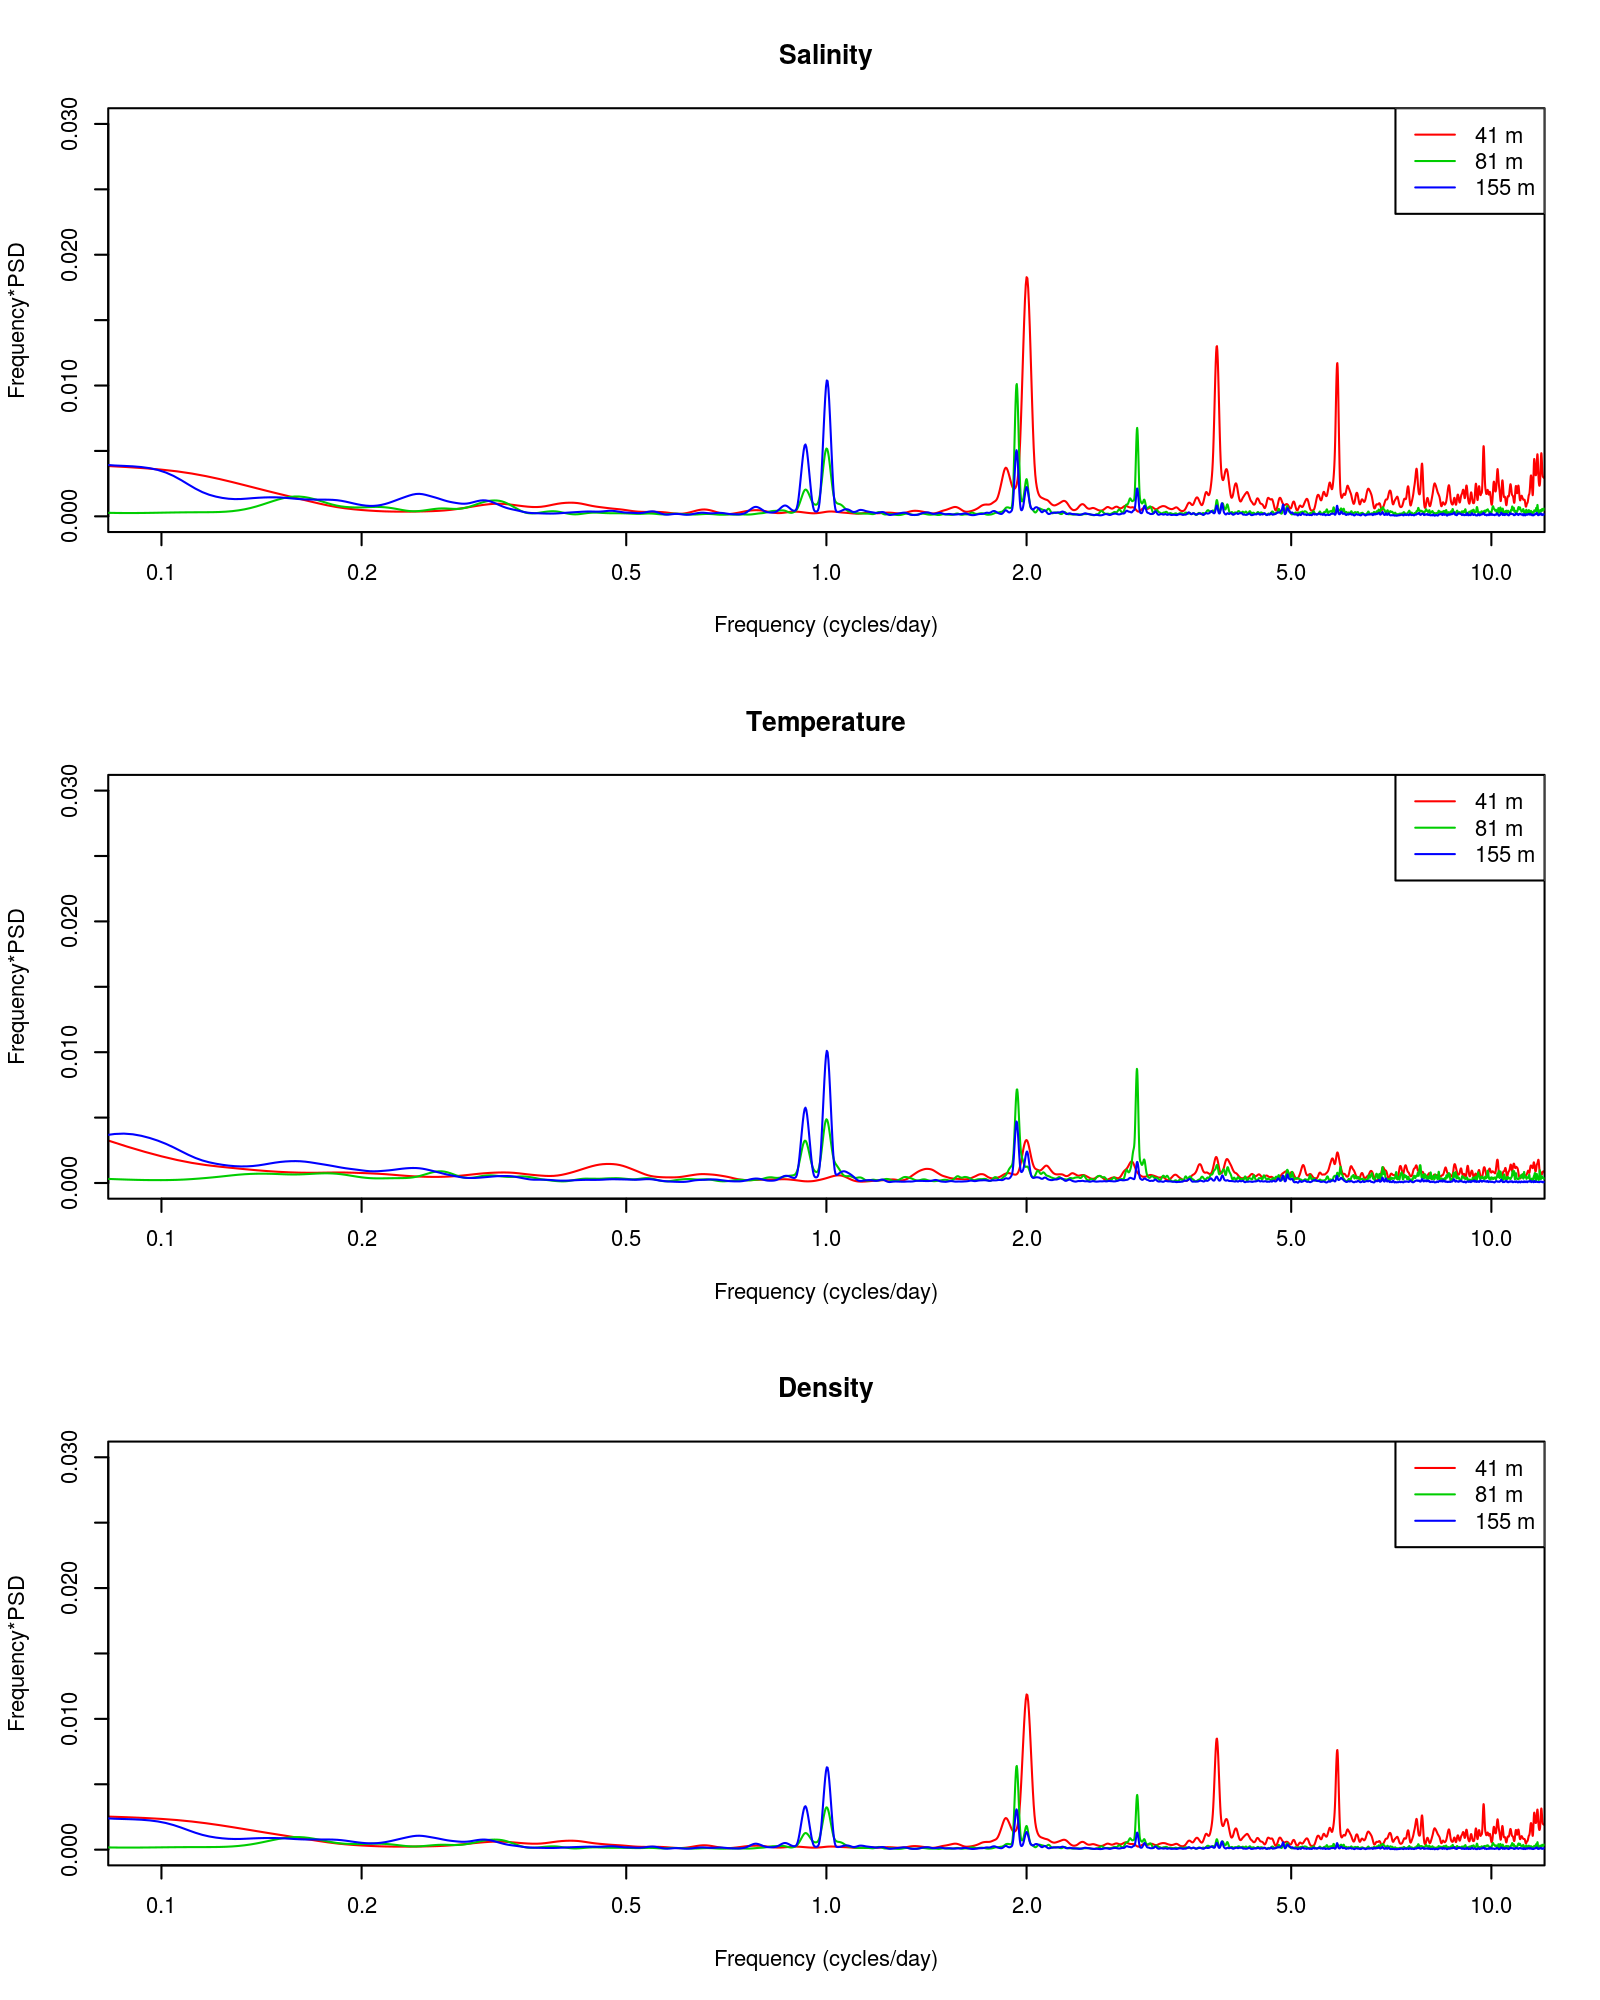
\includegraphics[width = 0.8\textwidth]{./figures/12_mctd_ps_2013_2014.png}
\caption[Power spectra of moored CTD, 2013-2014]{Power spectra of moored CTD data, August 2013 - August 2014.}
\label{f:mctd_ps_2013_2014}
\end{figure}

\begin{figure}
\centering
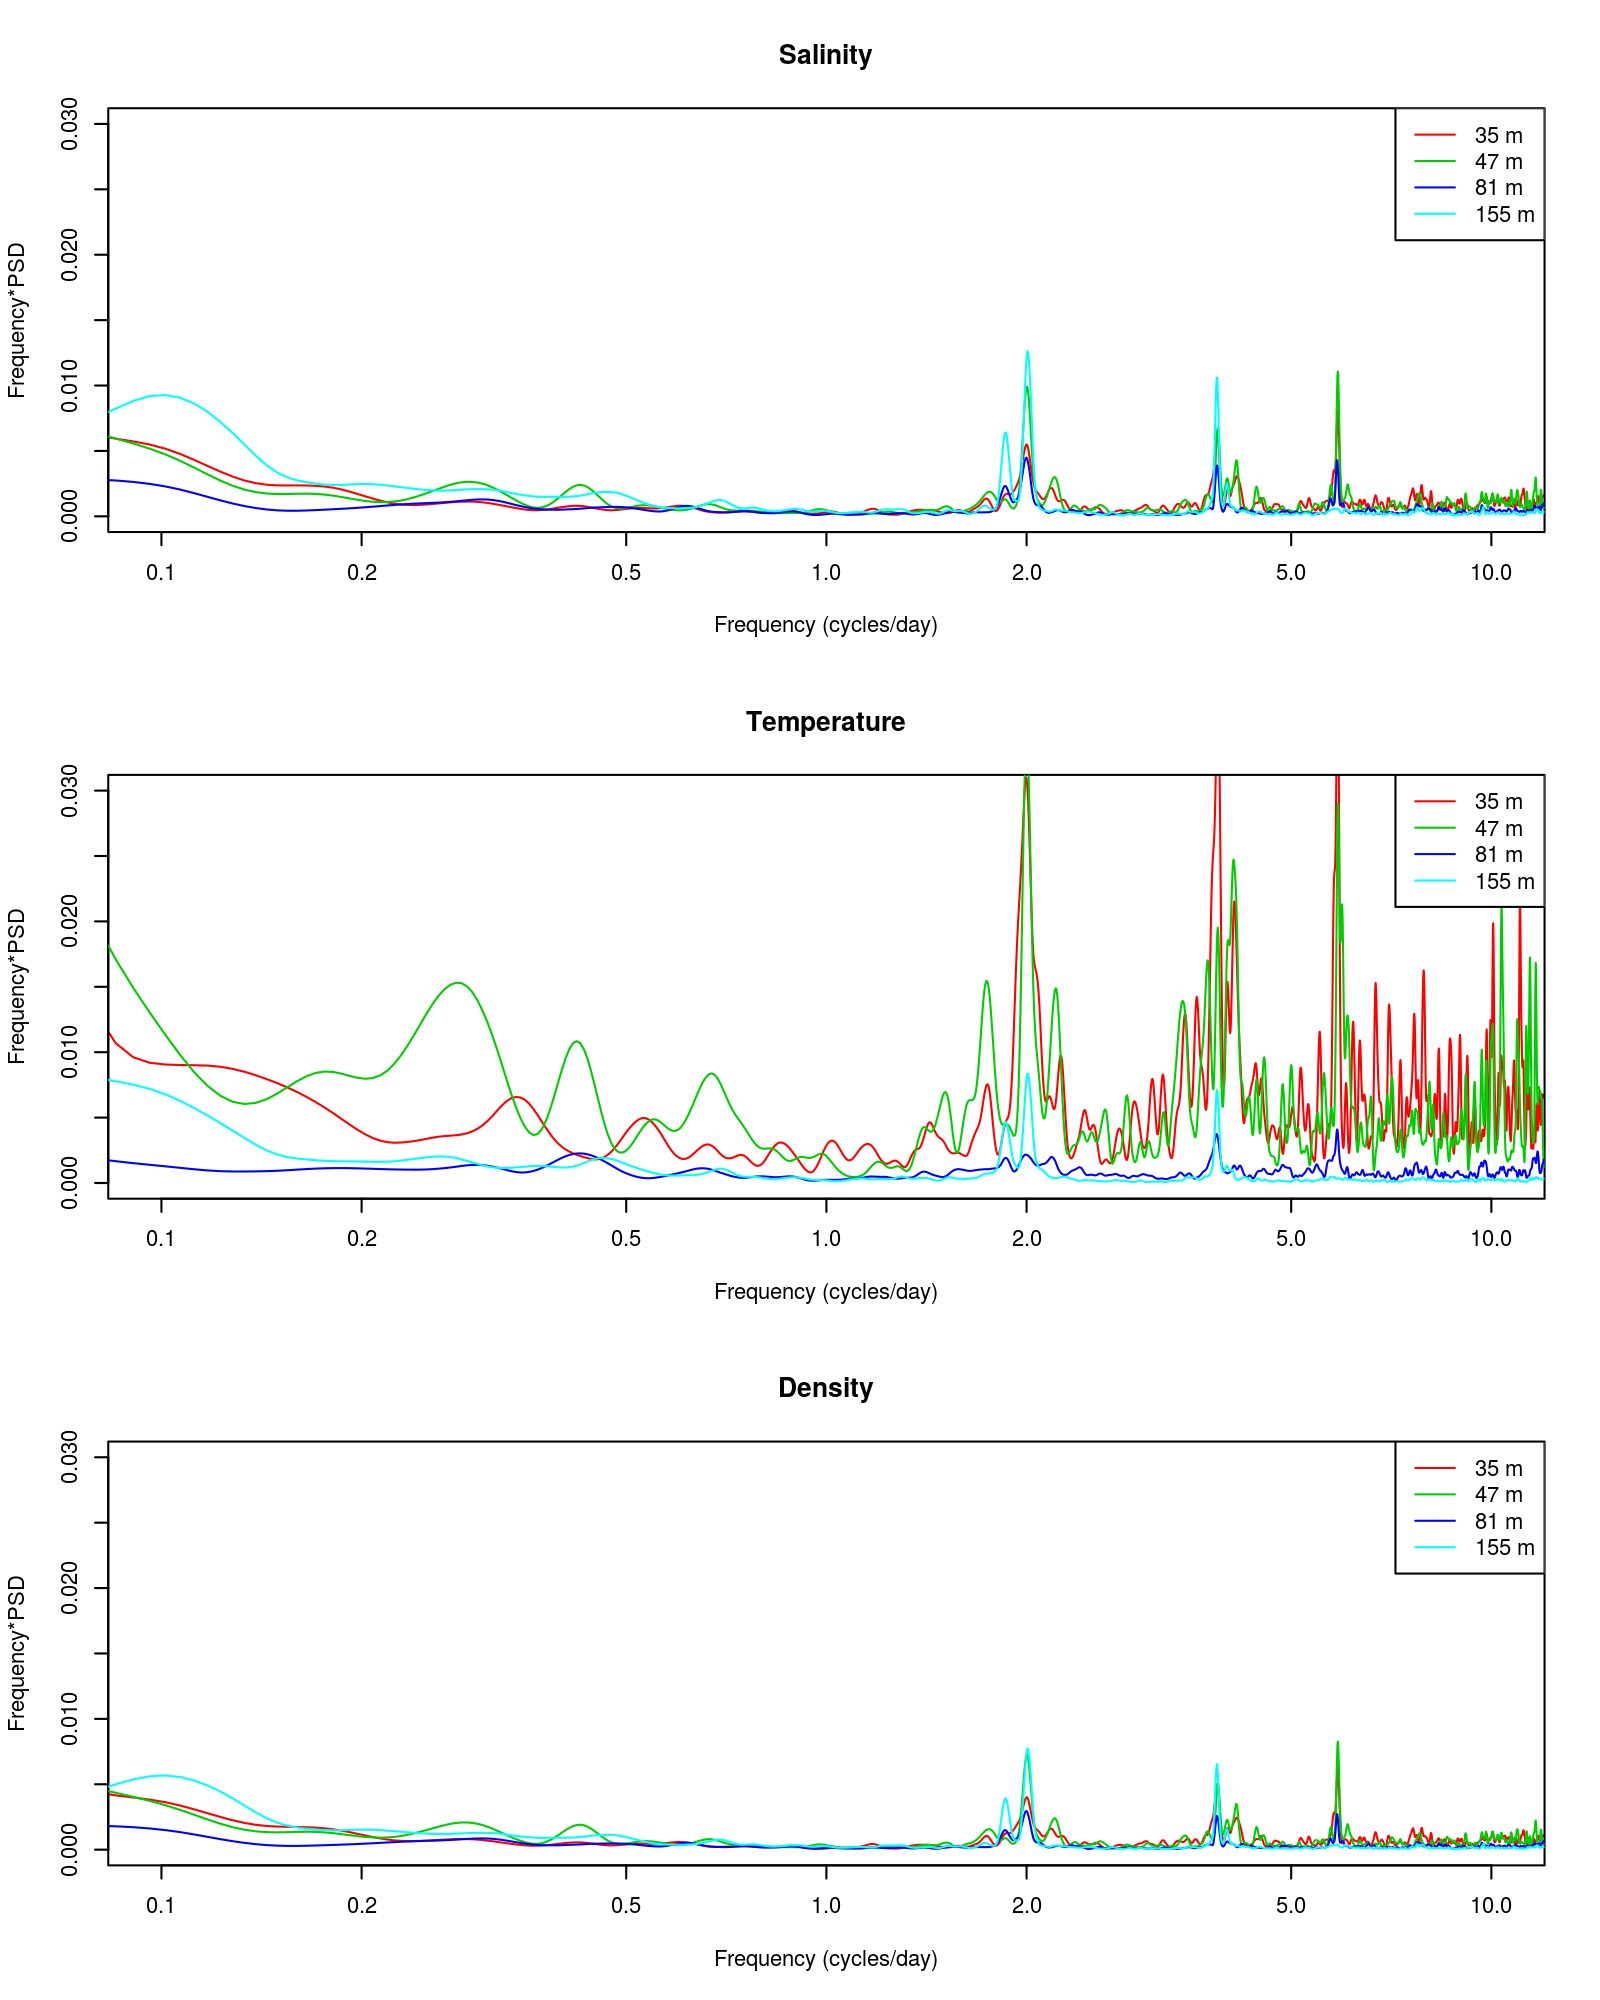
\includegraphics[width = 0.8\textwidth]{./figures/13_mctd_ps_2014_2015.png}
\caption[Power spectra of moored CTD, 2014-2015]{Power spectra of moored CTD data, August 2014 - August 2015.}
\label{f:mctd_ps_2014_2015}
\end{figure}

\begin{figure}  
\centering
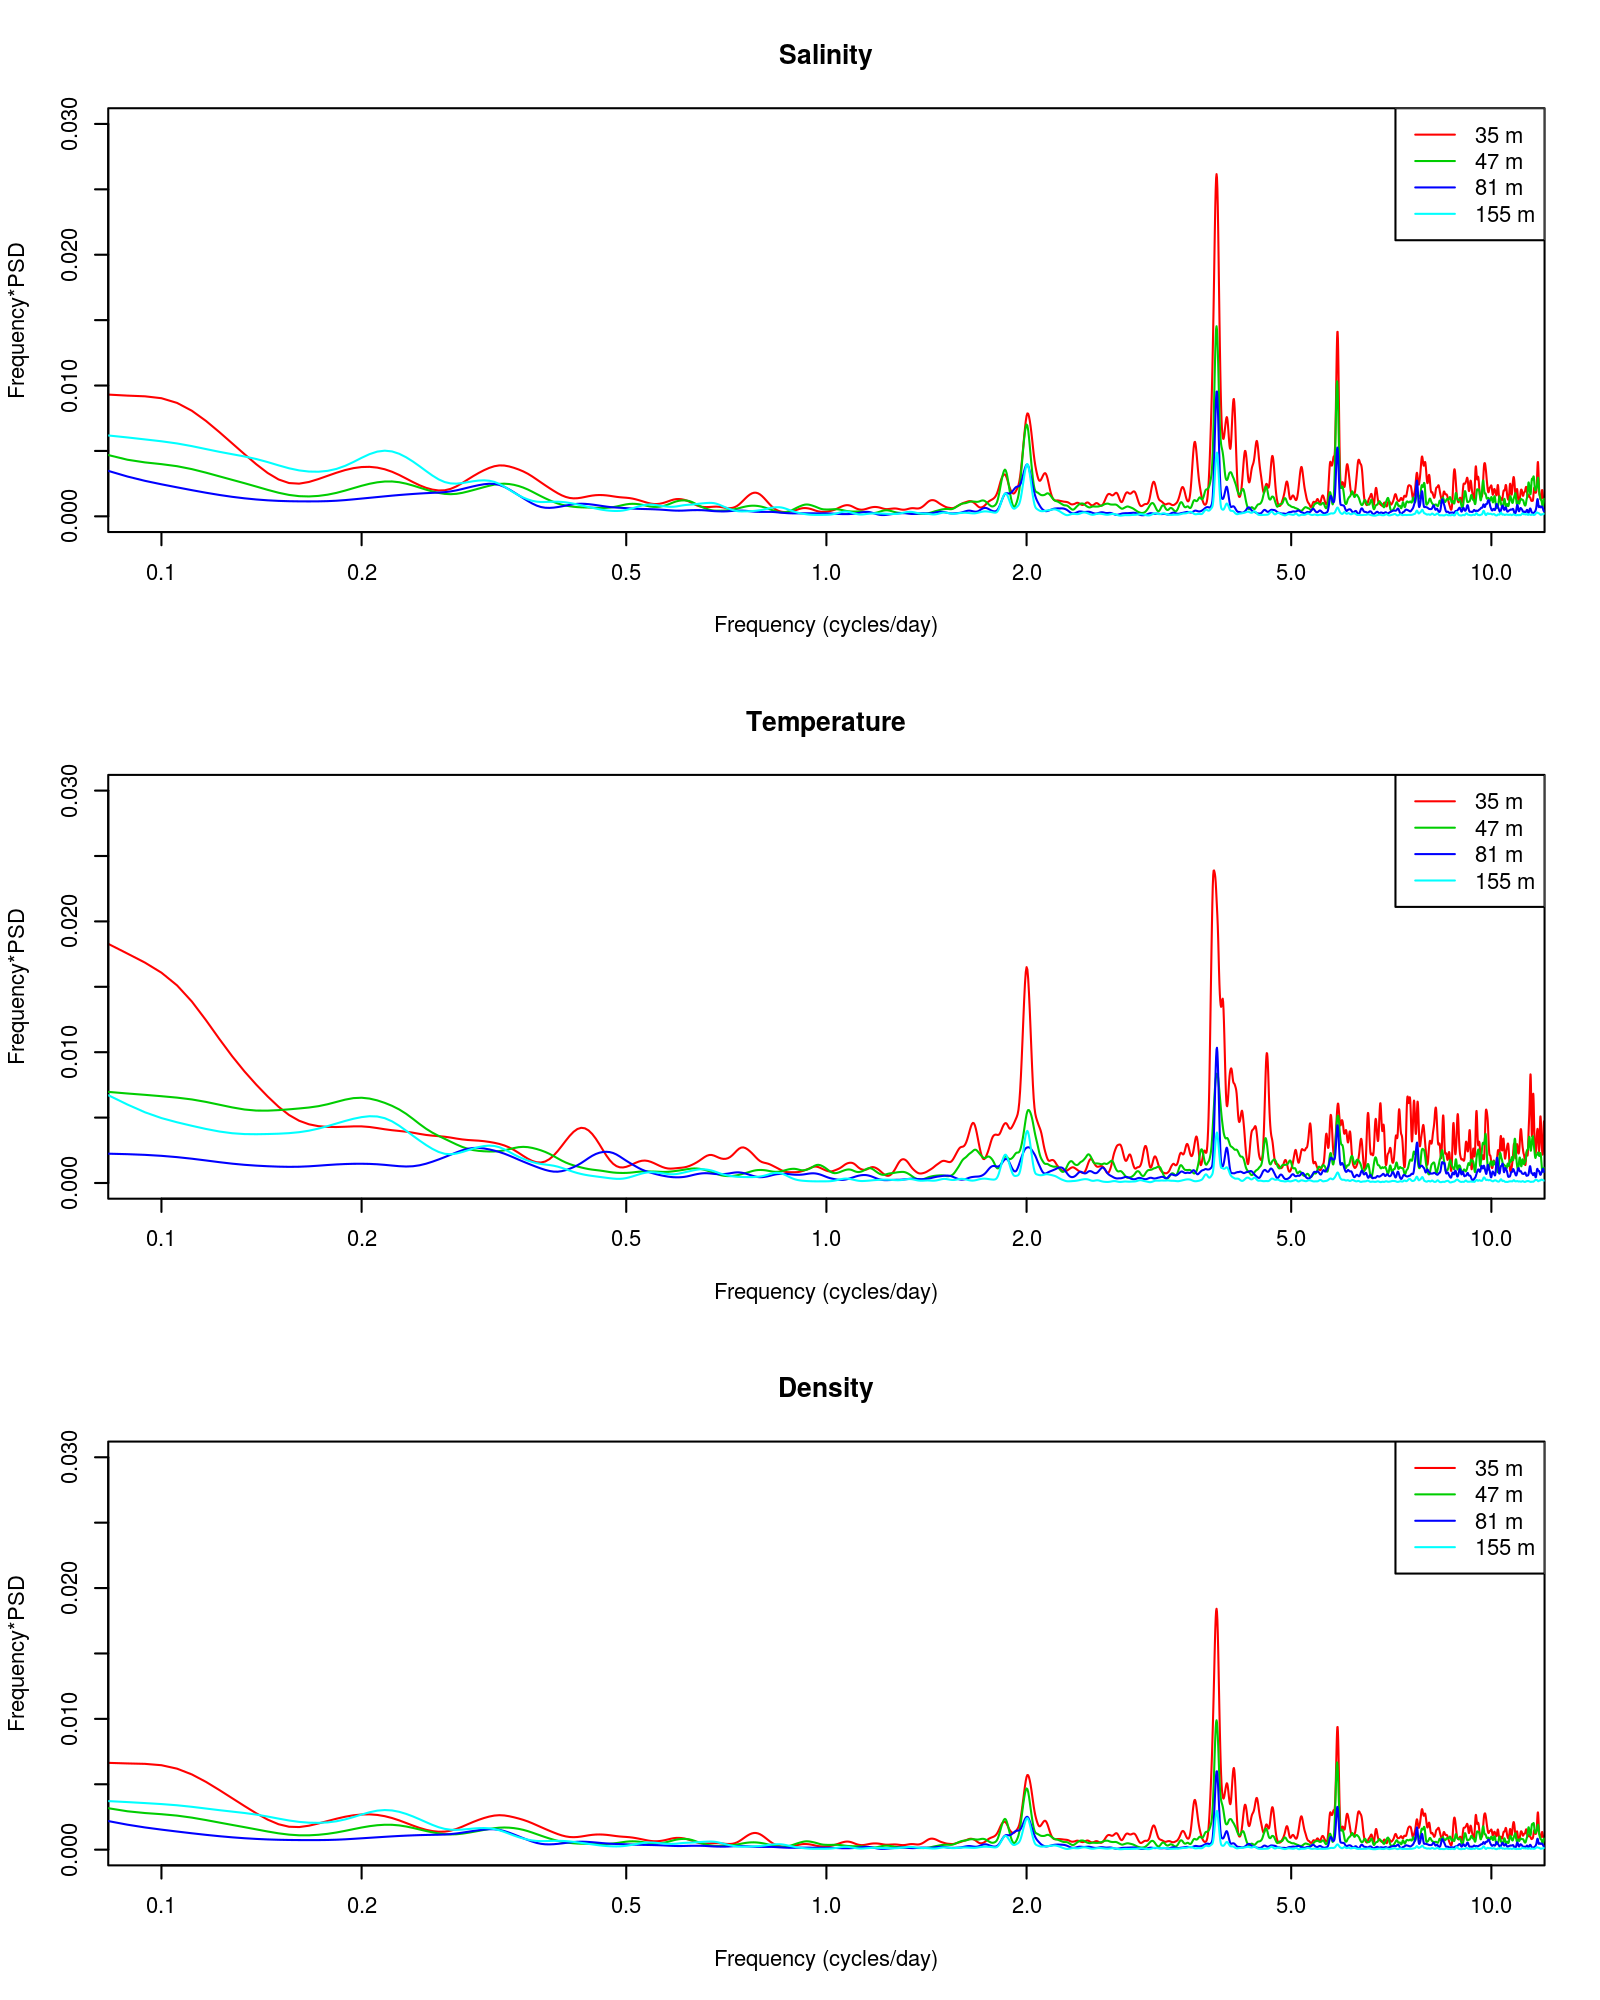
\includegraphics[width = 0.8\textwidth]{./figures/14_mctd_ps_2015_2016.png}
\caption[Power spectra of moored CTD, 2015-2016]{Power spectra of moored CTD data, August 2015 - August 2016.}
\label{f:mctd_ps_2015_2016}
\end{figure}



\begin{figure}  
\centering
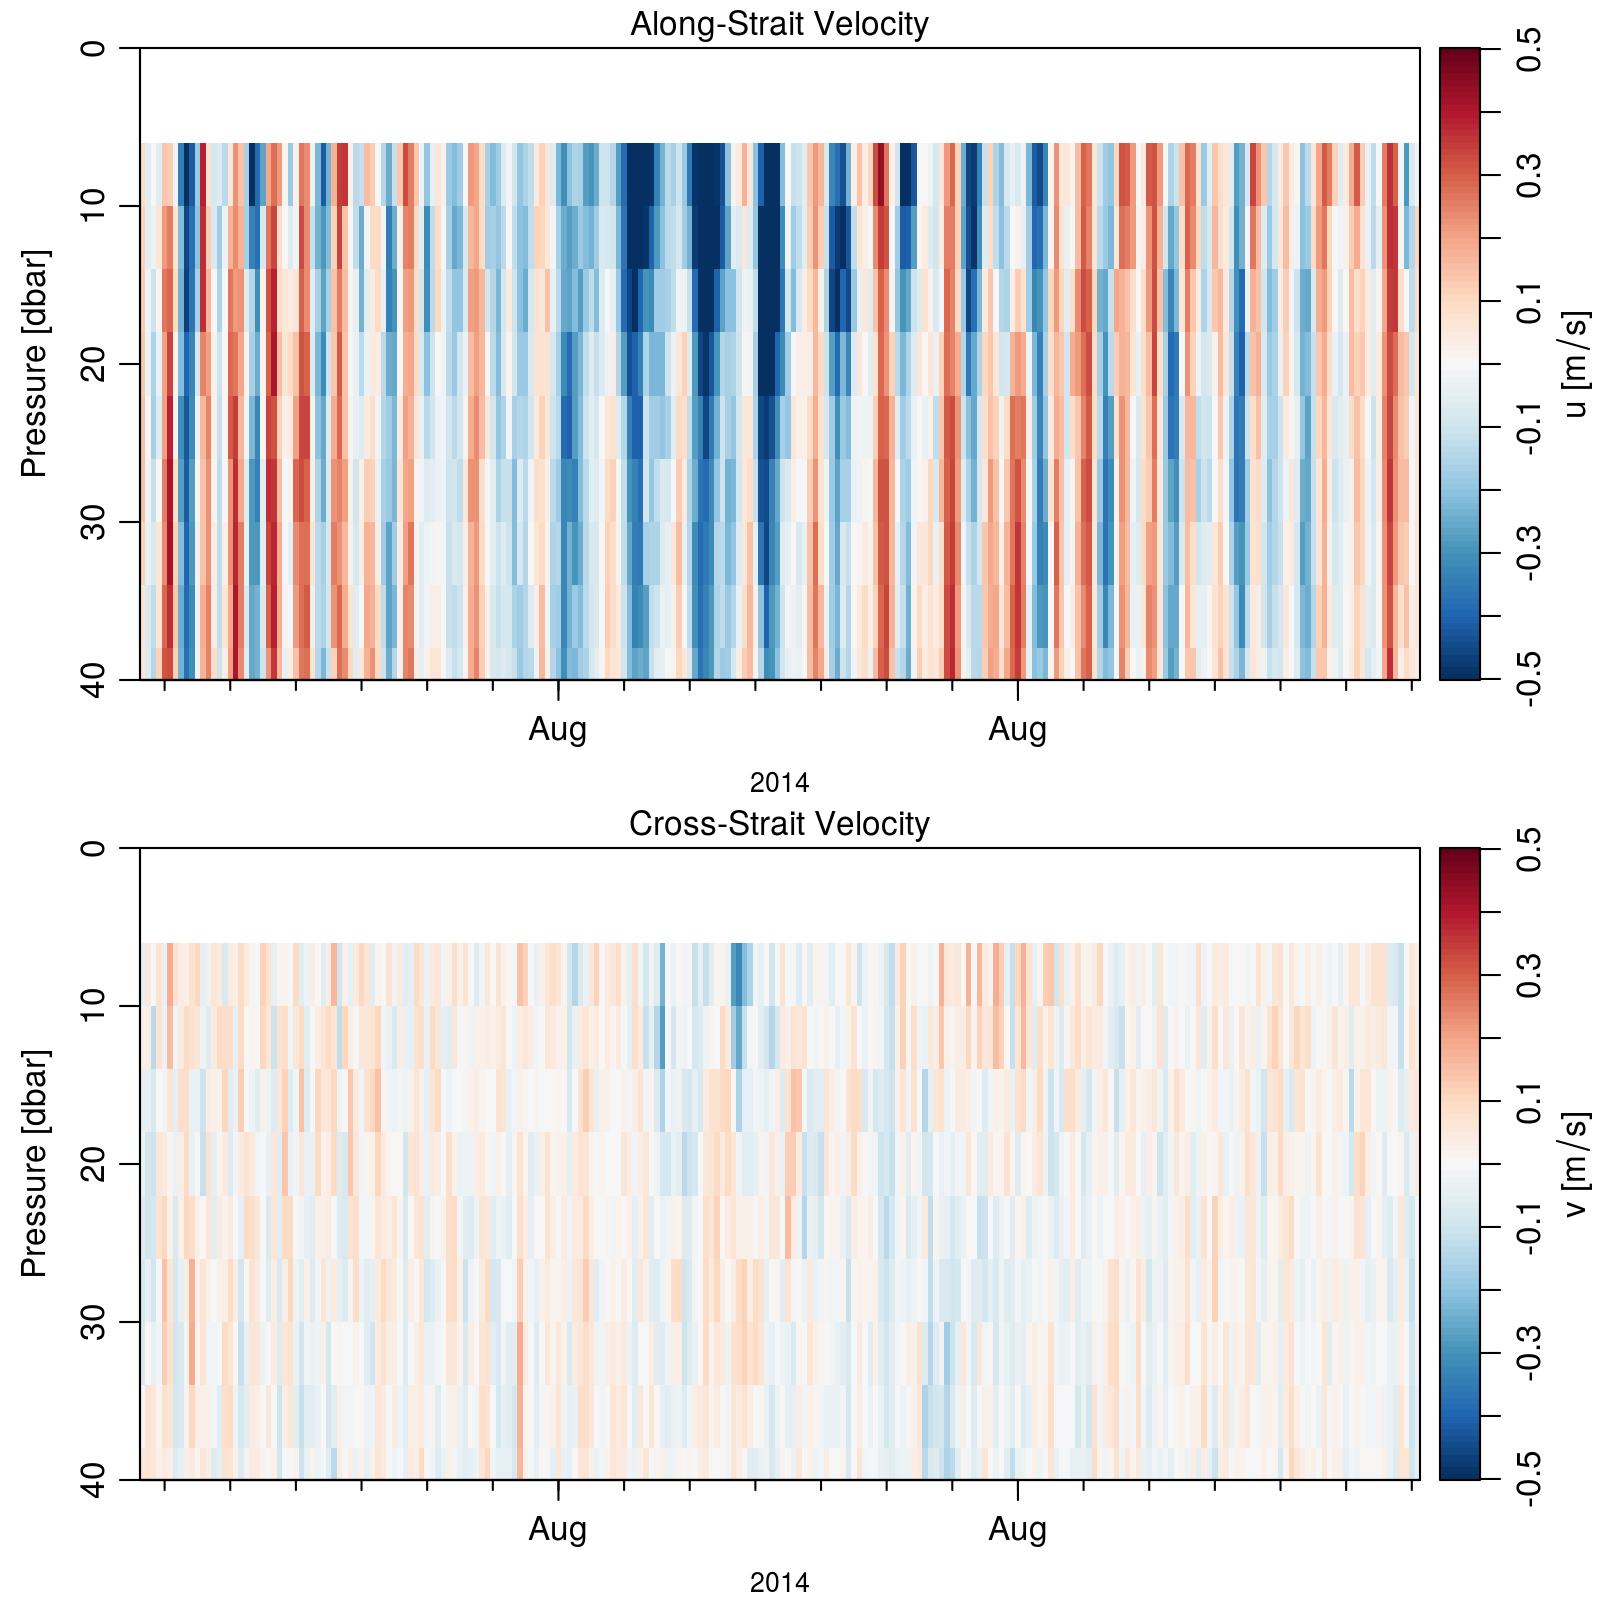
\includegraphics[width = 0.8\textwidth]{./figures/15_madcp_2014.png}
\caption[Bi-hourly ADCP data, Sept. 1 - Sept 30, 2014]{Bi-hourly moored ADCP data, September 1 2014 - September 30 2014.}
\label{f:madcp_sept2014}
\end{figure}


\begin{figure}  
\centering
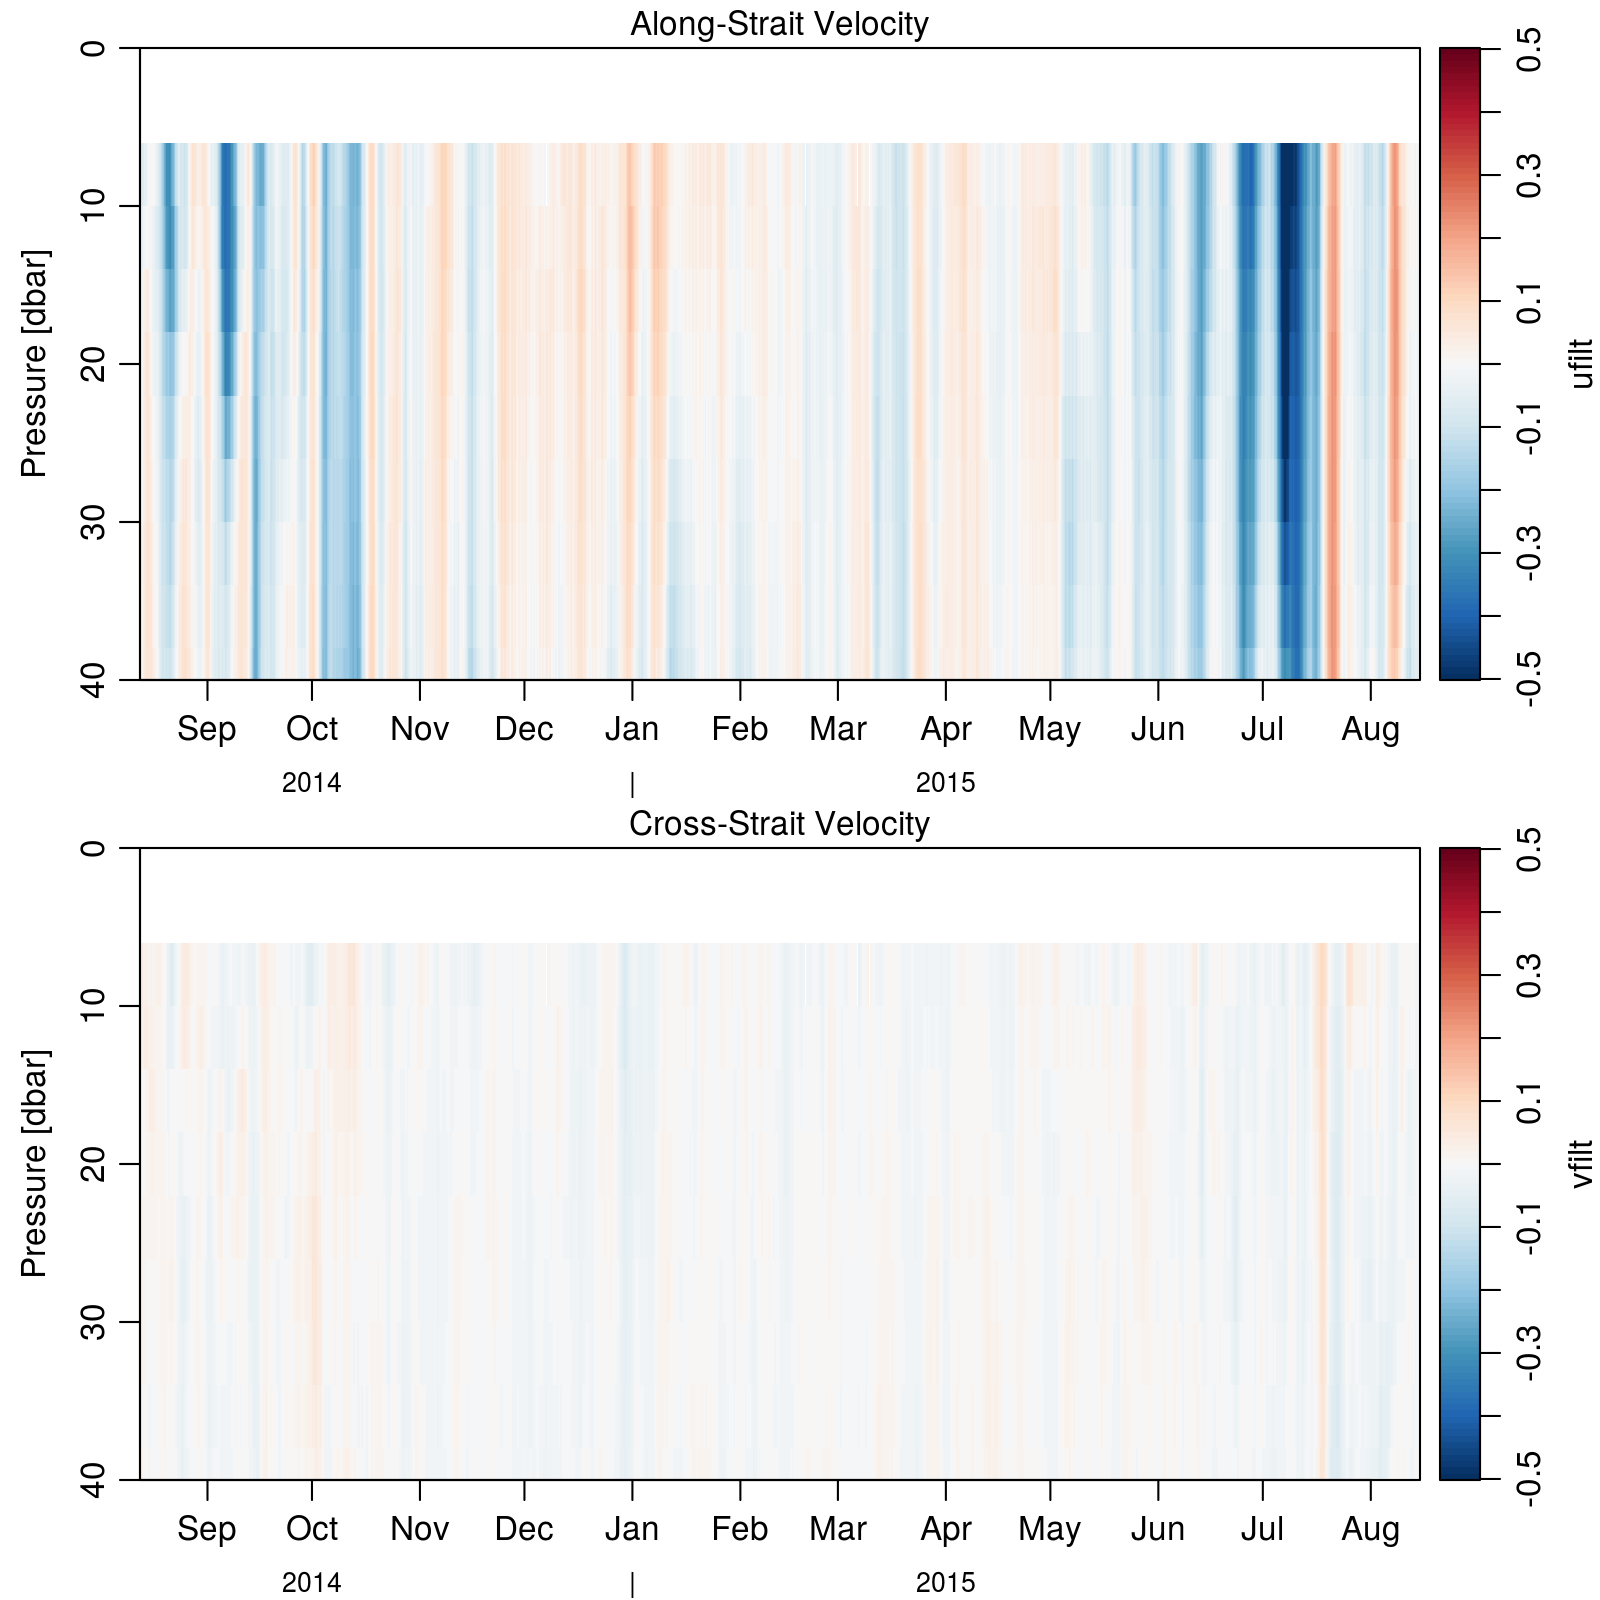
\includegraphics[width = 0.8\textwidth]{./figures/17_madcp_lpf_2014_2015.png}
\caption[Low-pass filtered ADCP data, 2014-2015]{Low-pass filtered ADCP data, August 2014 - August 2015}
\label{f:madcp_lpf_2014_2015}
\end{figure}

\begin{figure}  
\centering
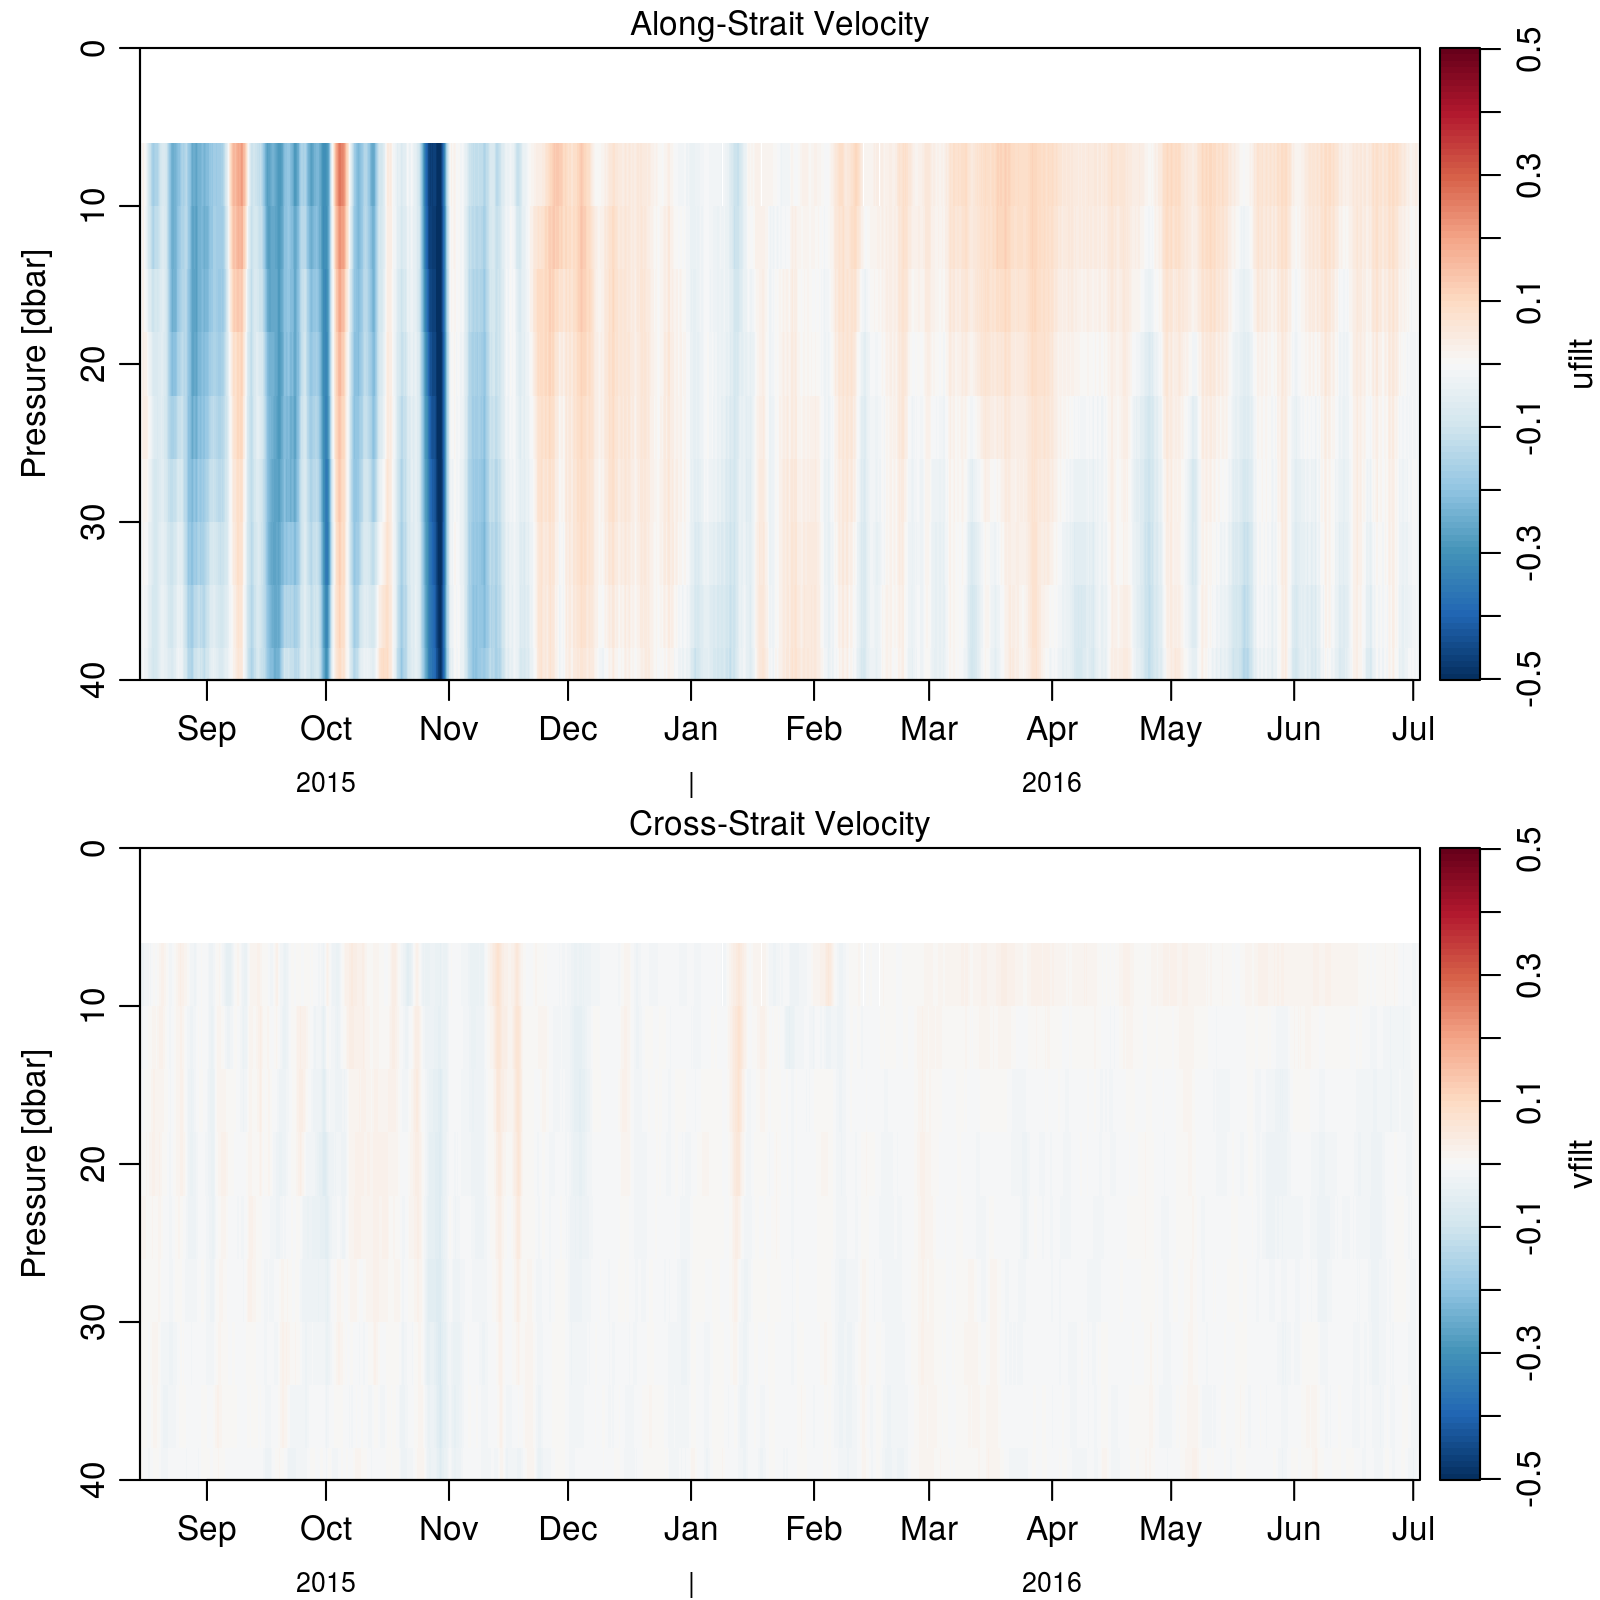
\includegraphics[width = 0.8\textwidth]{./figures/18_madcp_lpf_2015_2016.png}
\caption[Low-pass filtered ADCP data, 2015-2016]{Low-pass filtered ADCP data, August 2015 - August 2016}
\label{f:madcp_lpf_2015_2016}
\end{figure}



\pagebreak
\newpage

\begin{figure}  
\centering
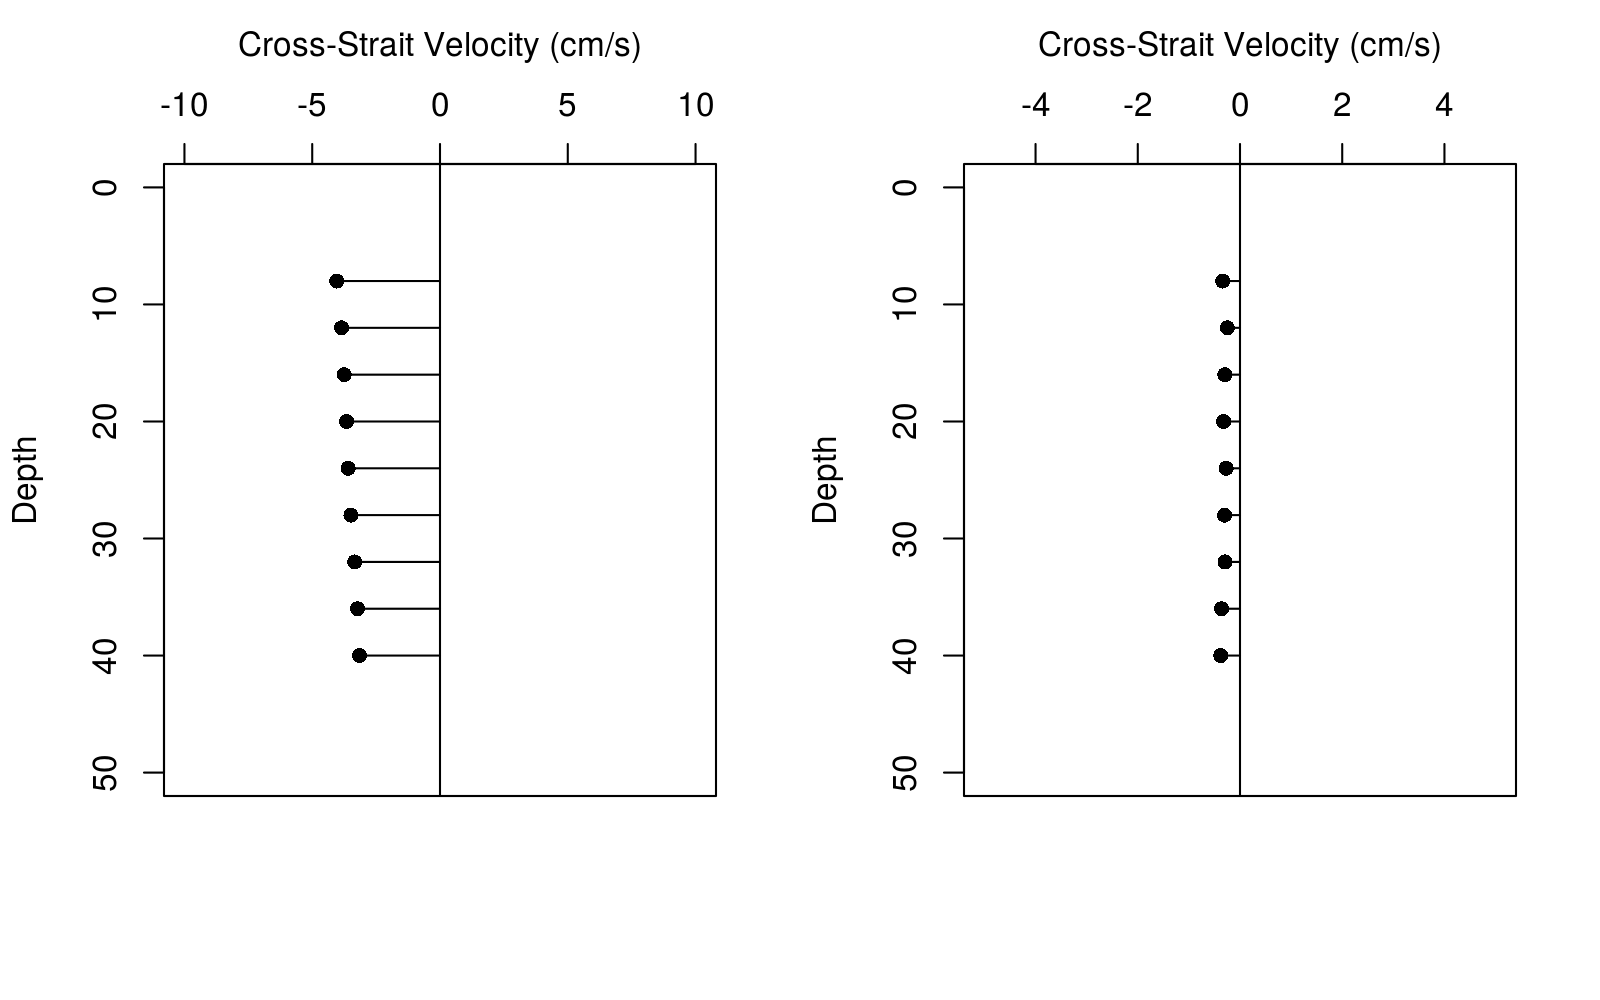
\includegraphics[width = 0.8\textwidth]{./figures/36_amf_2014_2015.png}
\caption[Mean flow, 2014-2015]{Mean flow, August 2014 - August 2015}
\label{f:amf_2014_2015}
\end{figure}

\begin{figure}  
\centering
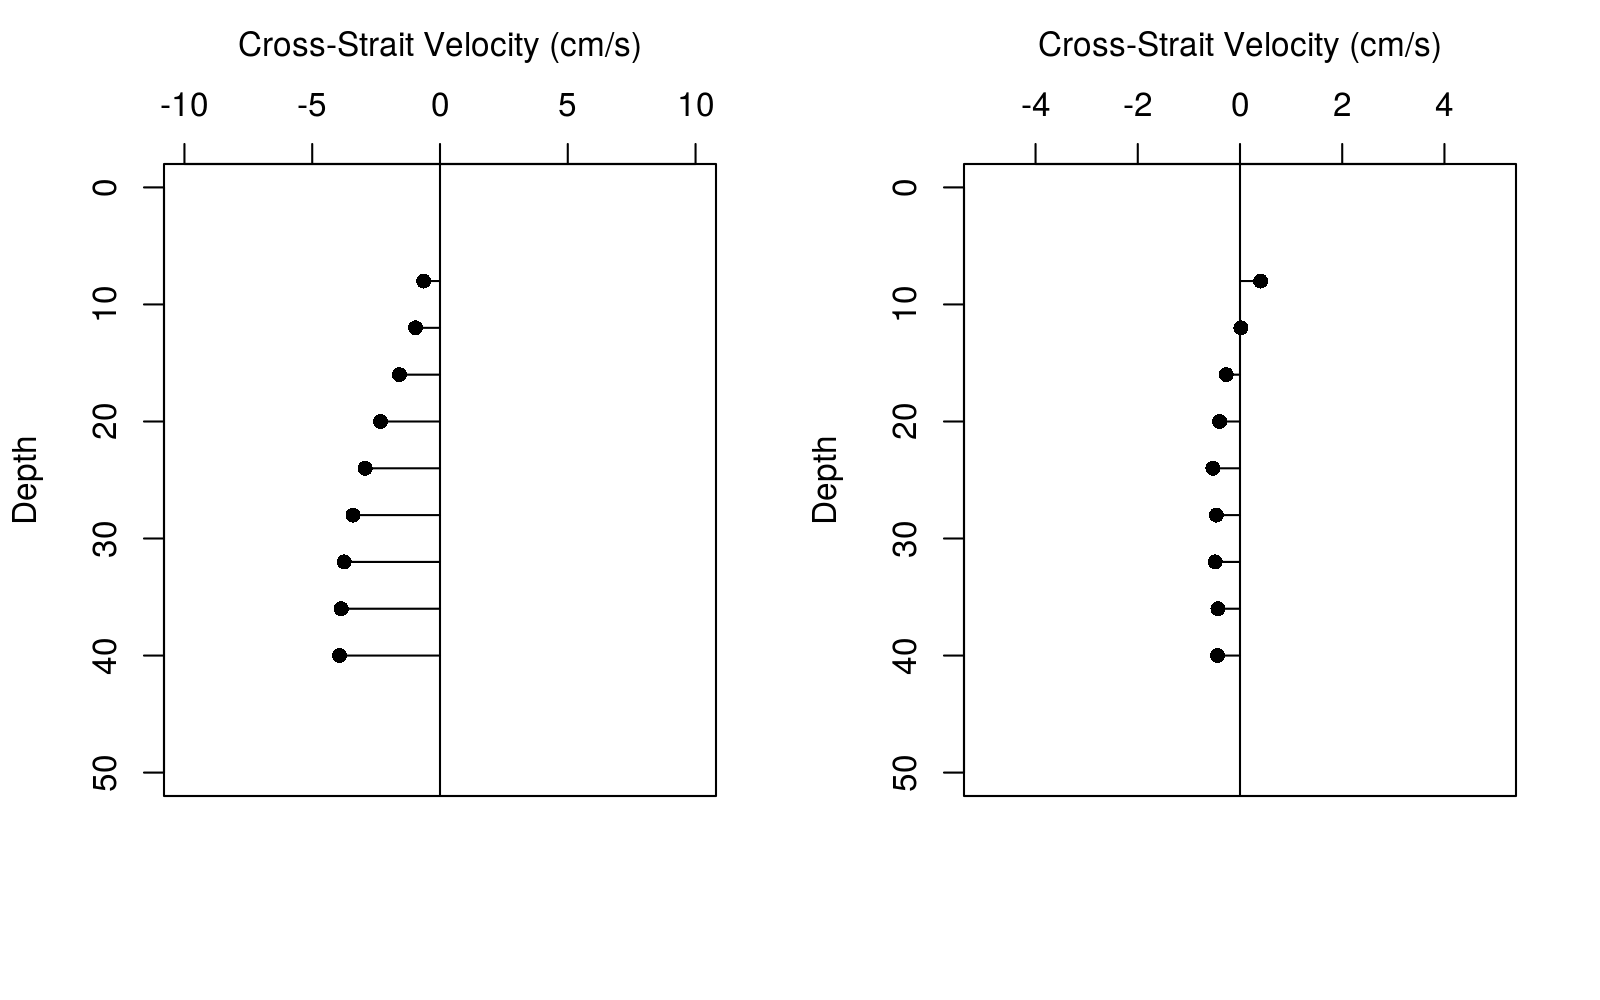
\includegraphics[width = 0.8\textwidth]{./figures/37_amf_2015_2016.png}
\caption[Mean flow, 2015-2016]{Mean flow,, August 2015 - August 2016}
\label{f:amf_2015_2016}
\end{figure}


\begin{figure}  
\centering
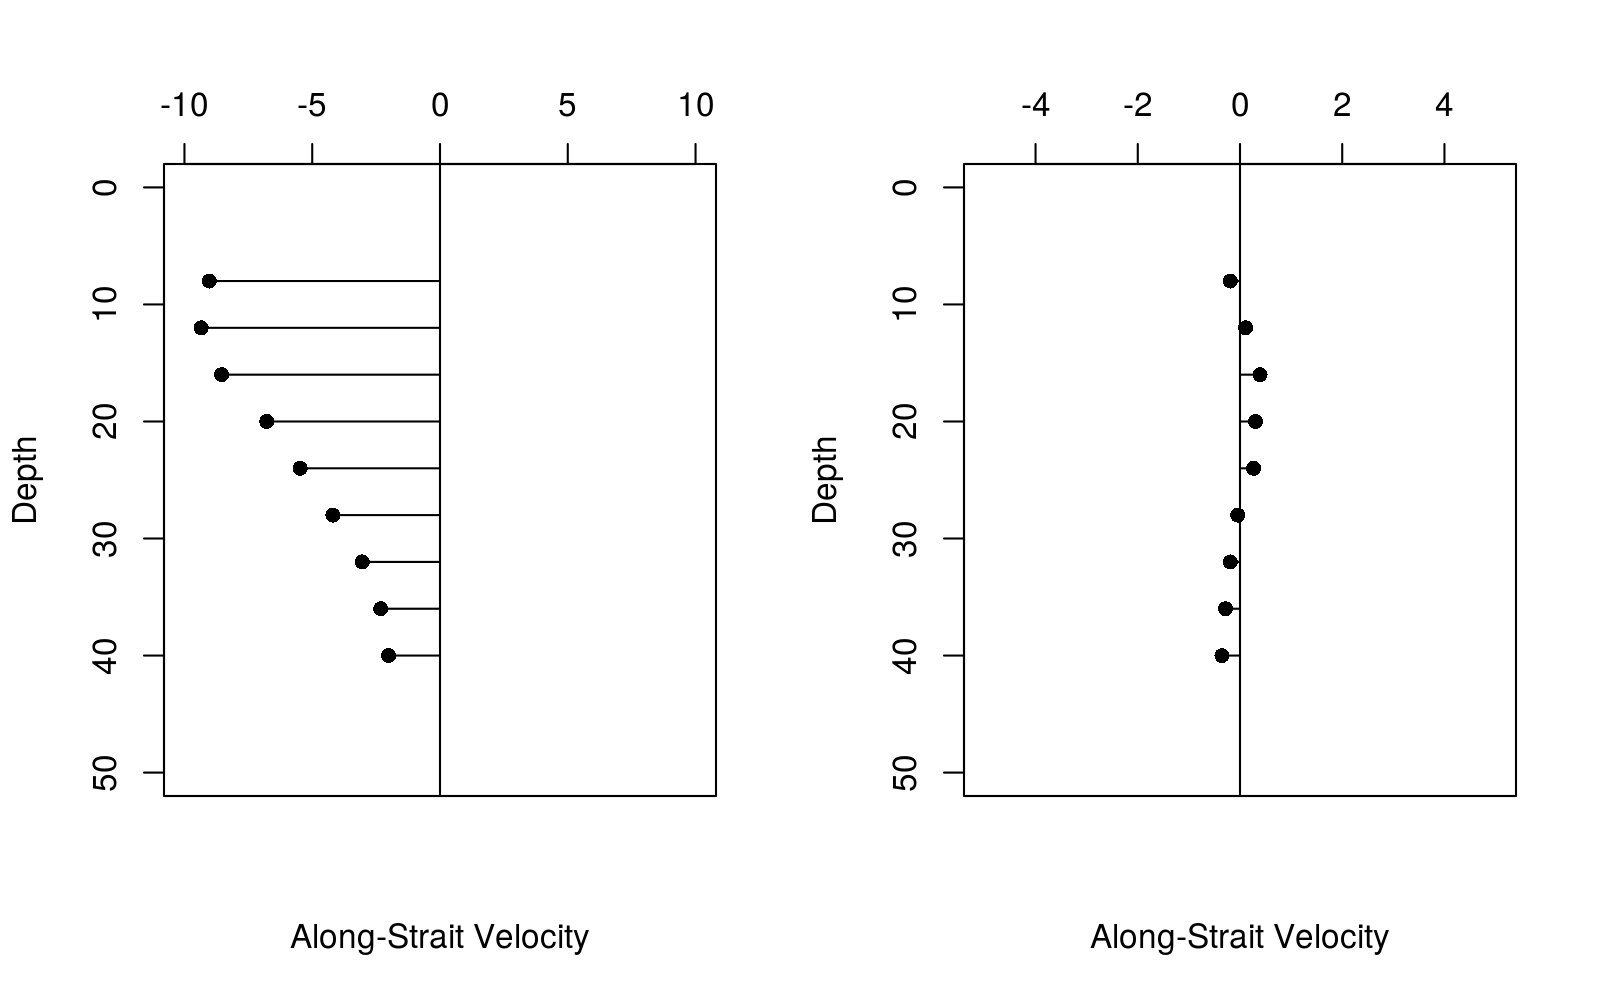
\includegraphics[width = 0.8\textwidth]{./figures/38_smf_lateSummer_2014.png}
\caption[Mean flow, Late Summer, 2014]{Mean flow, Late Summer: August 2014 to September 2014}
\label{f:smf_ls_2014}
\end{figure}

\begin{figure}  
\centering
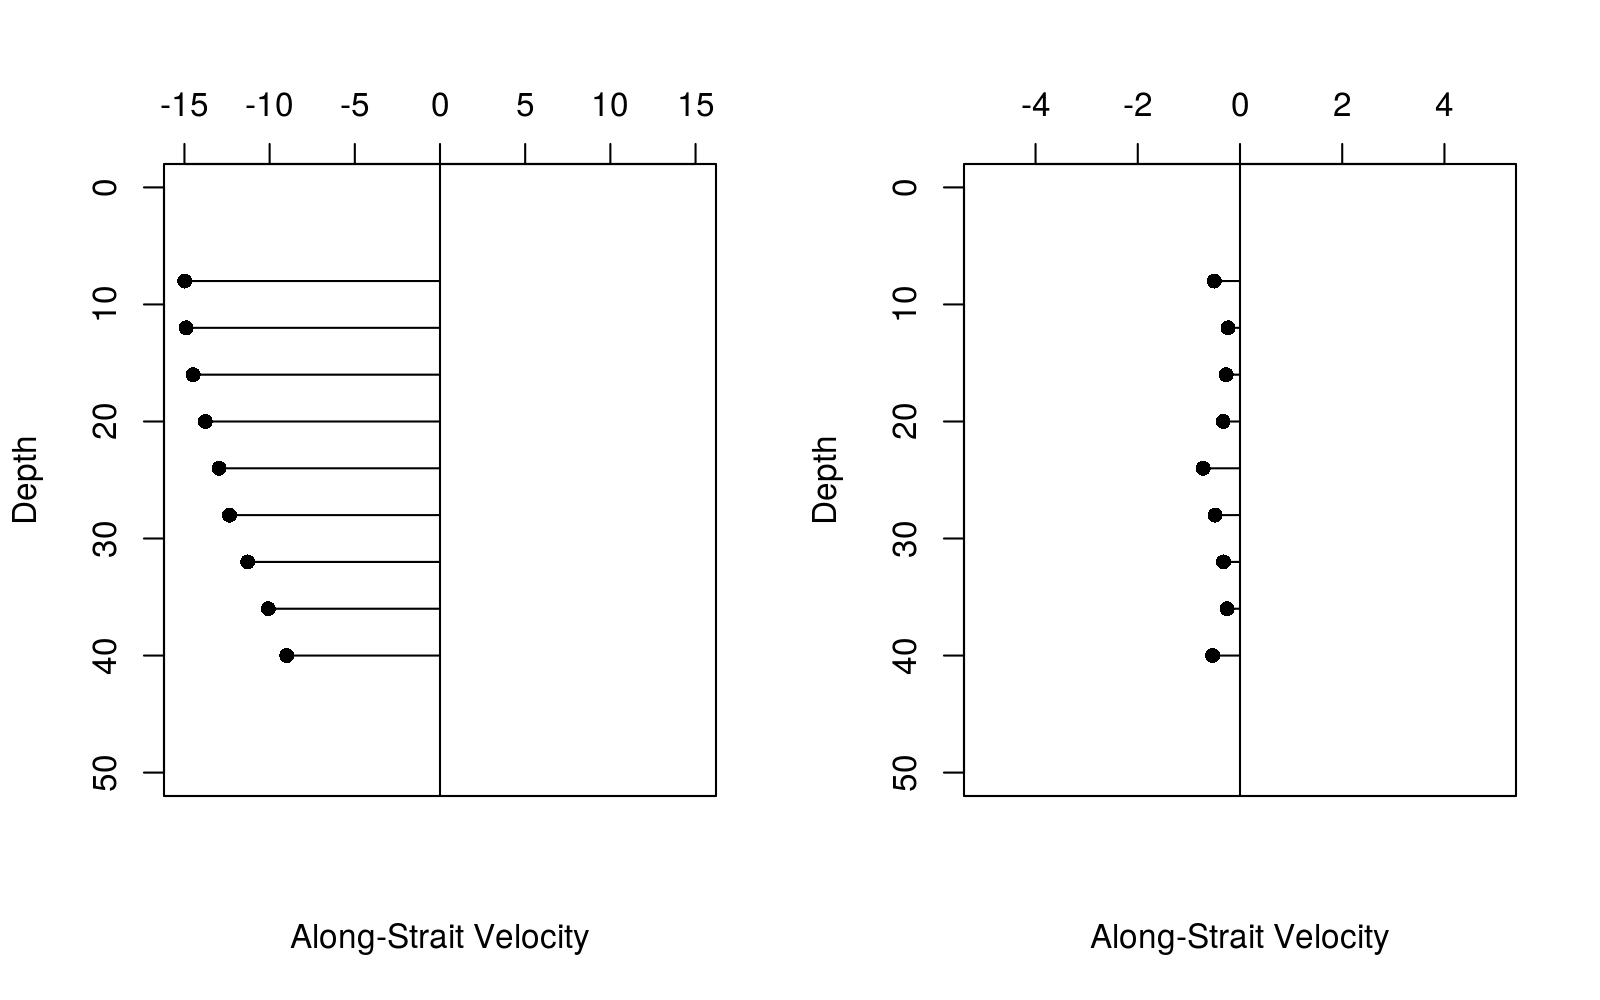
\includegraphics[width = 0.8\textwidth]{./figures/39_smf_lateSummer_2015.png}
\caption[Mean flow, Late Summer, 2015]{Mean flow, Late Summer: August 2015 to September 2015}
\label{f:smf_ls_2015}
\end{figure}


\begin{figure}  
\centering
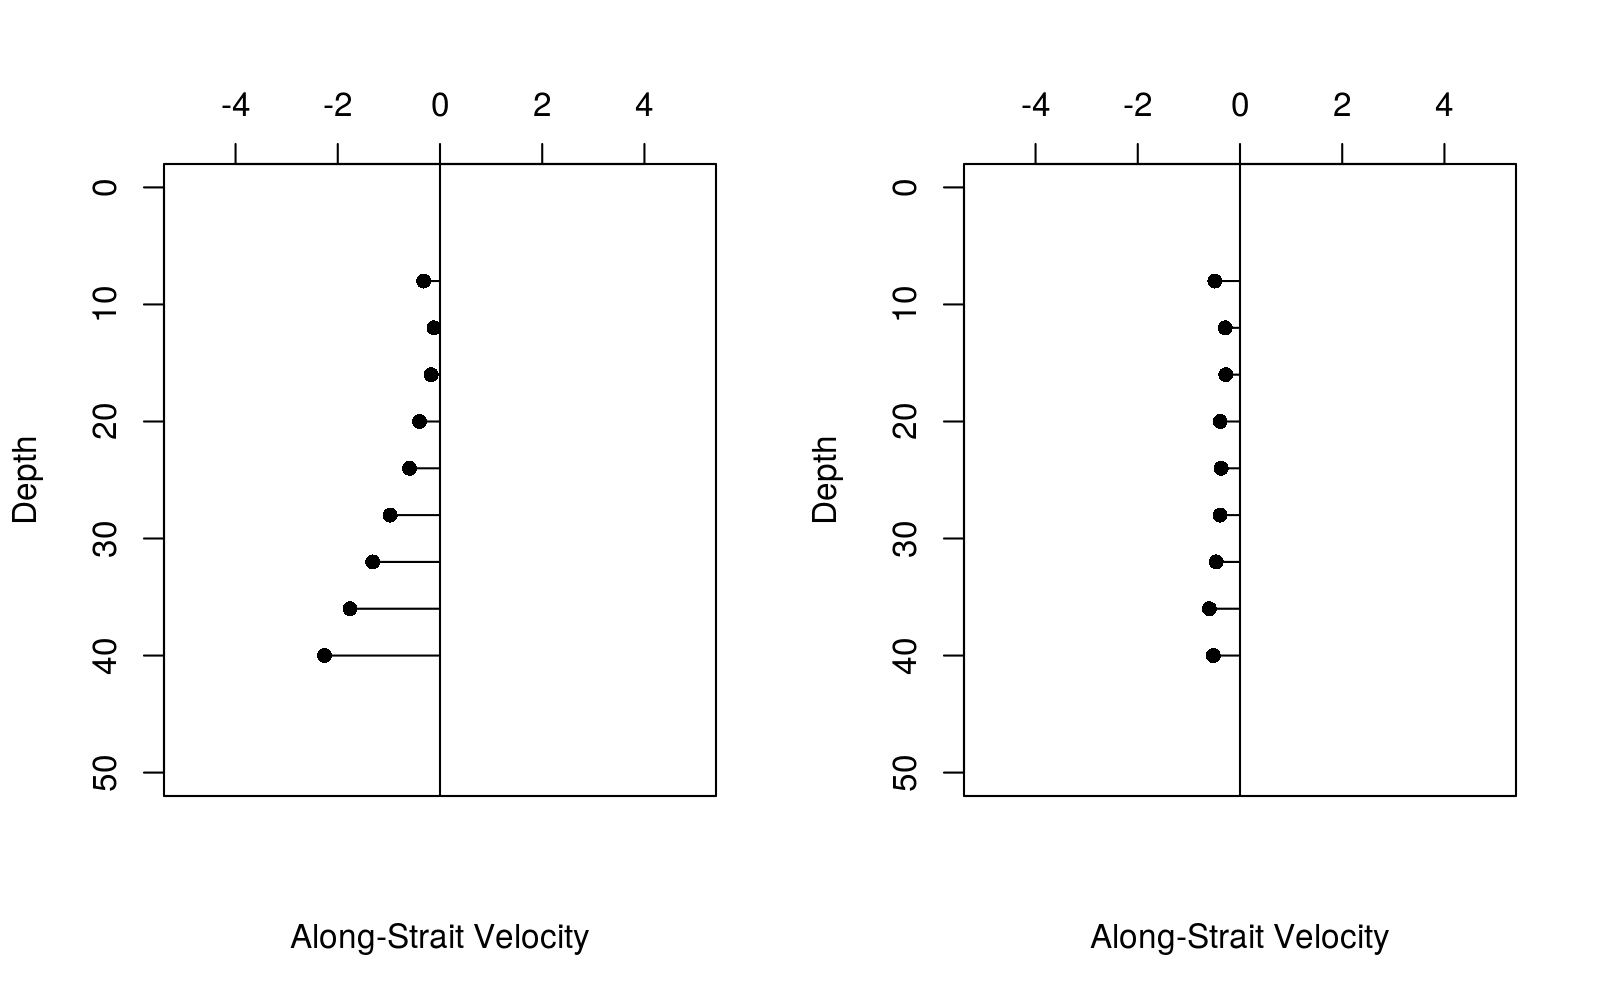
\includegraphics[width = 0.8\textwidth]{./figures/40_smf_fall_2014.png}
\caption[Mean flow, Fall, 2014]{Mean flow, Fall: October 2014 - December 2014}
\label{f:smf_f_2014}
\end{figure}

\begin{figure}  
\centering
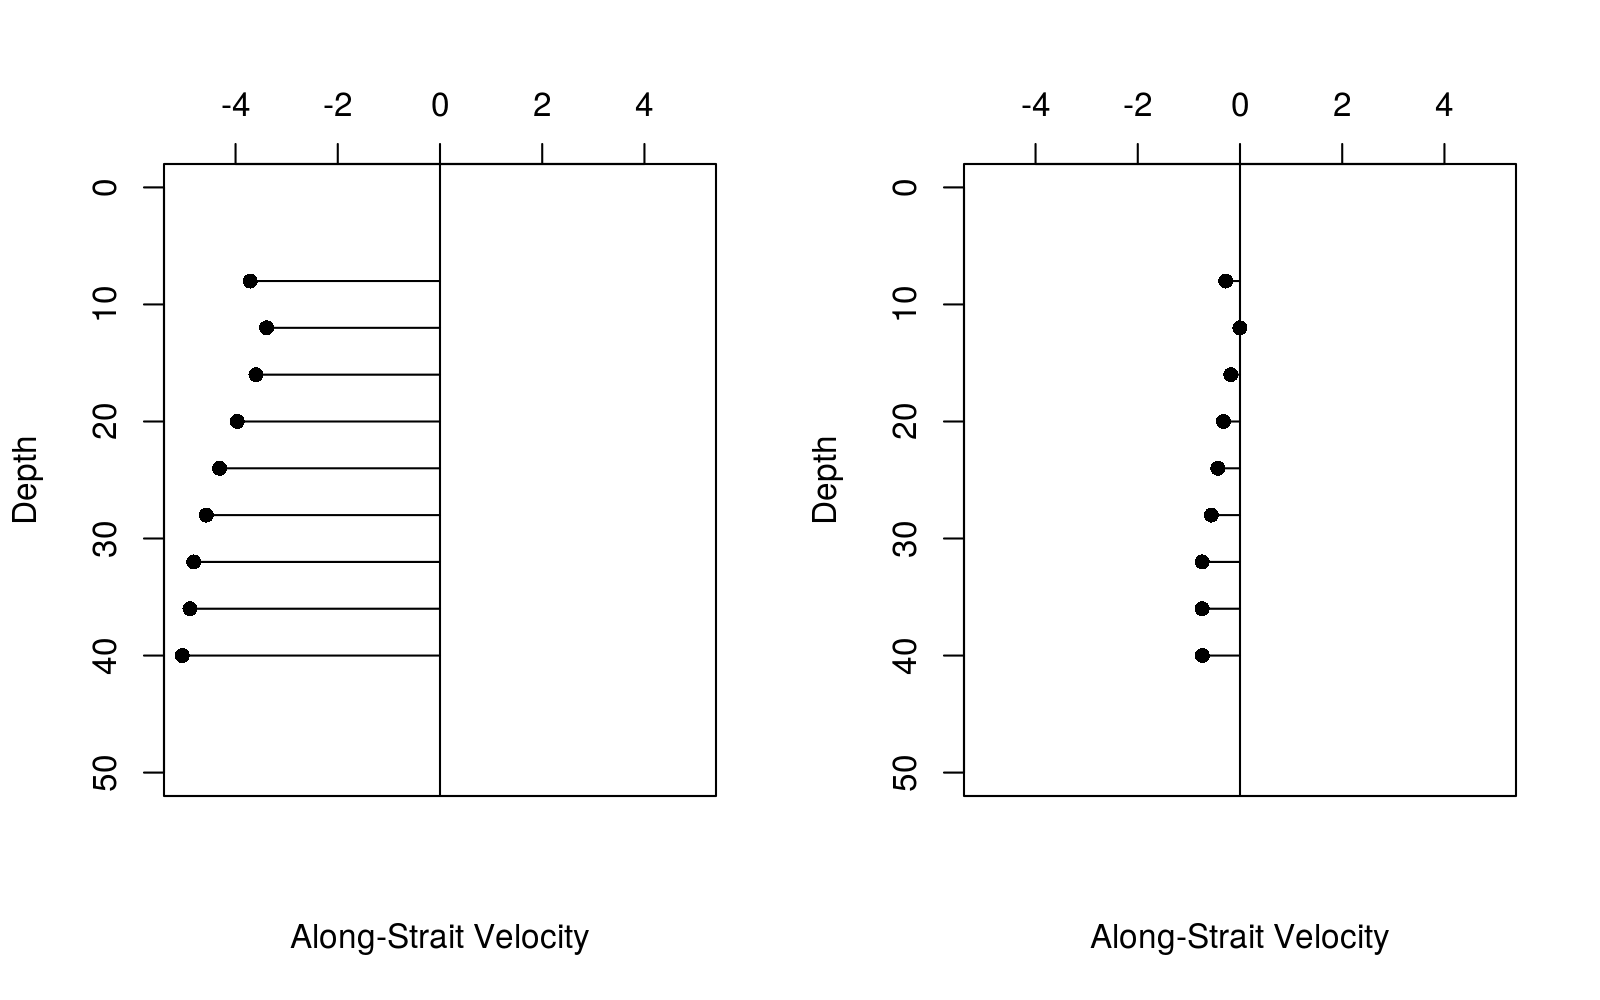
\includegraphics[width = 0.8\textwidth]{./figures/41_smf_fall_2015.png}
\caption[Mean flow, Fall, 2015]{Mean flow, Fall: October 2015 - December 2015}
\label{f:smf_f_2015}
\end{figure}


\begin{figure}  
\centering
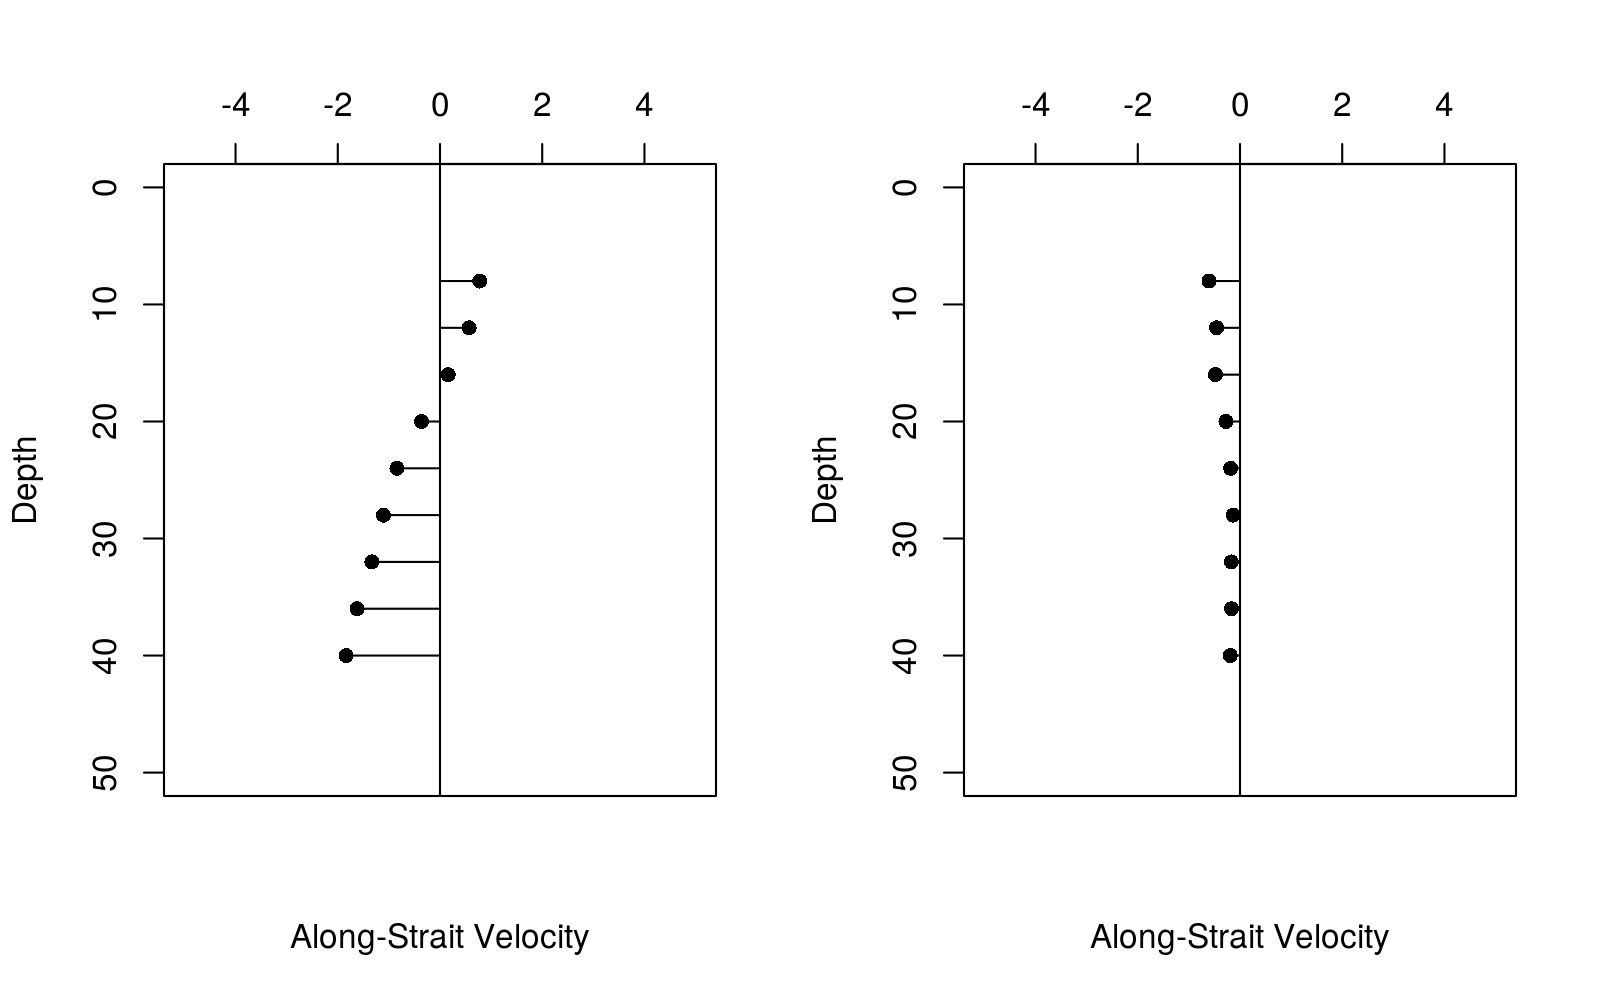
\includegraphics[width = 0.8\textwidth]{./figures/42_smf_winter_2015.png}
\caption[Mean flow, Winter, 2015]{Mean flow, Winter: January 2015 - March 2015}
\label{f:smf_w_2015}
\end{figure}

\begin{figure}  
\centering
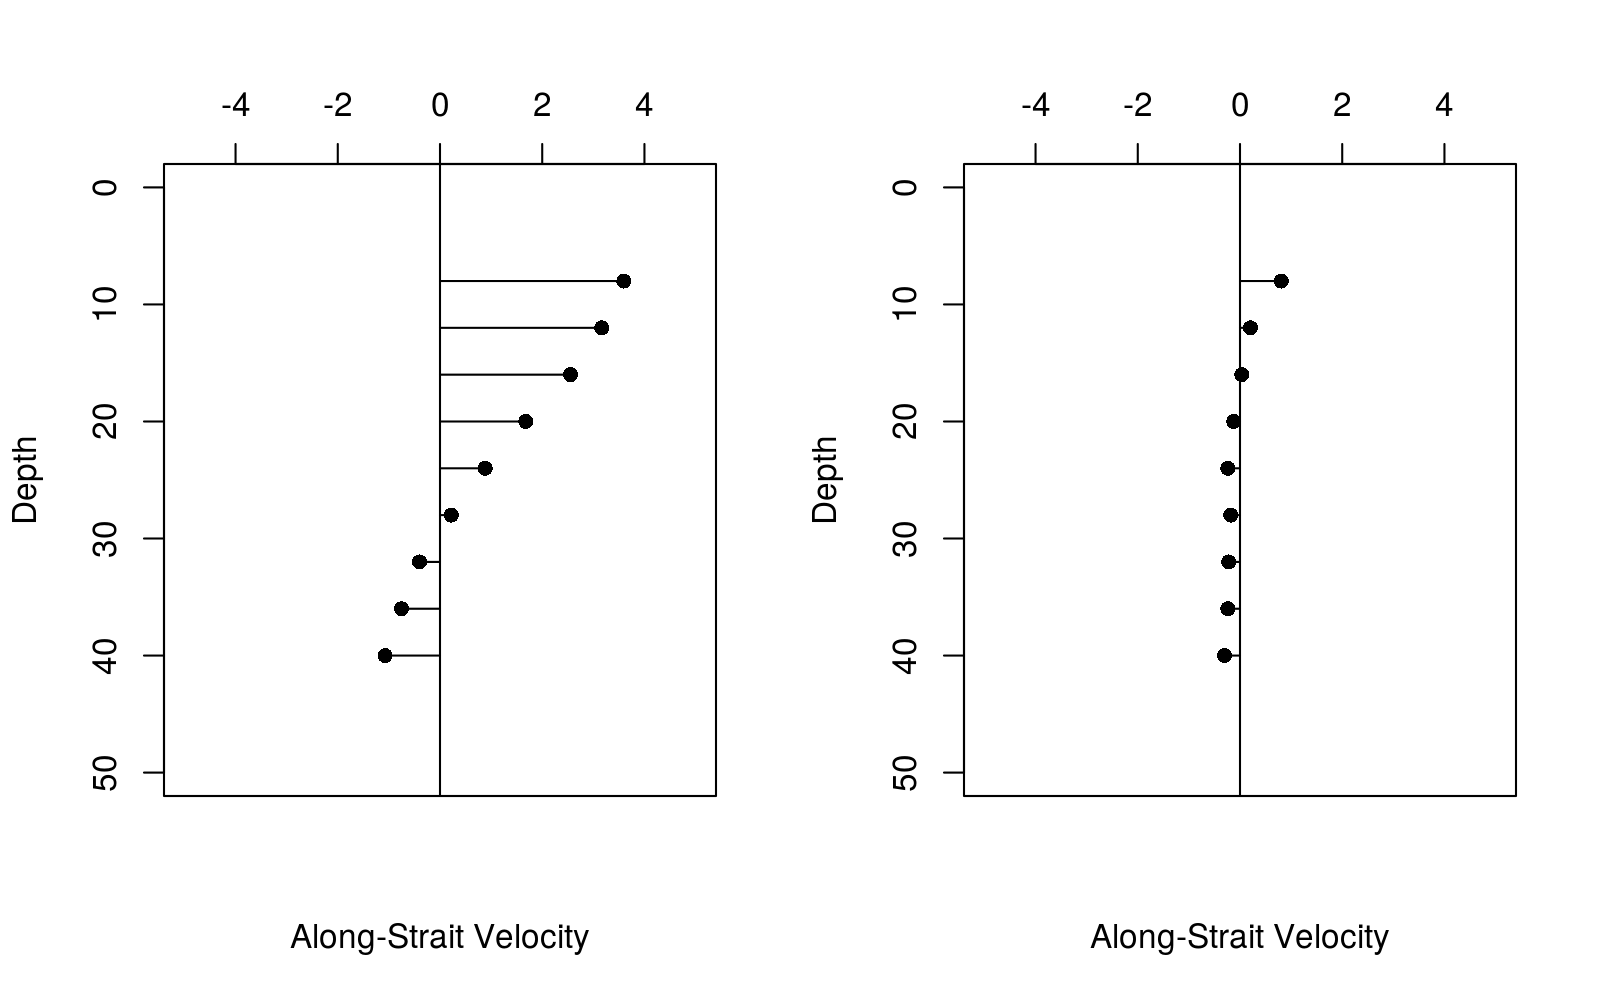
\includegraphics[width = 0.8\textwidth]{./figures/43_smf_winter_2016.png}
\caption[Mean flow, Winter, 2016]{Mean flow, Winter: January 2016 - March 2016}
\label{f:smf_w_2016}
\end{figure}


\begin{figure}  
\centering
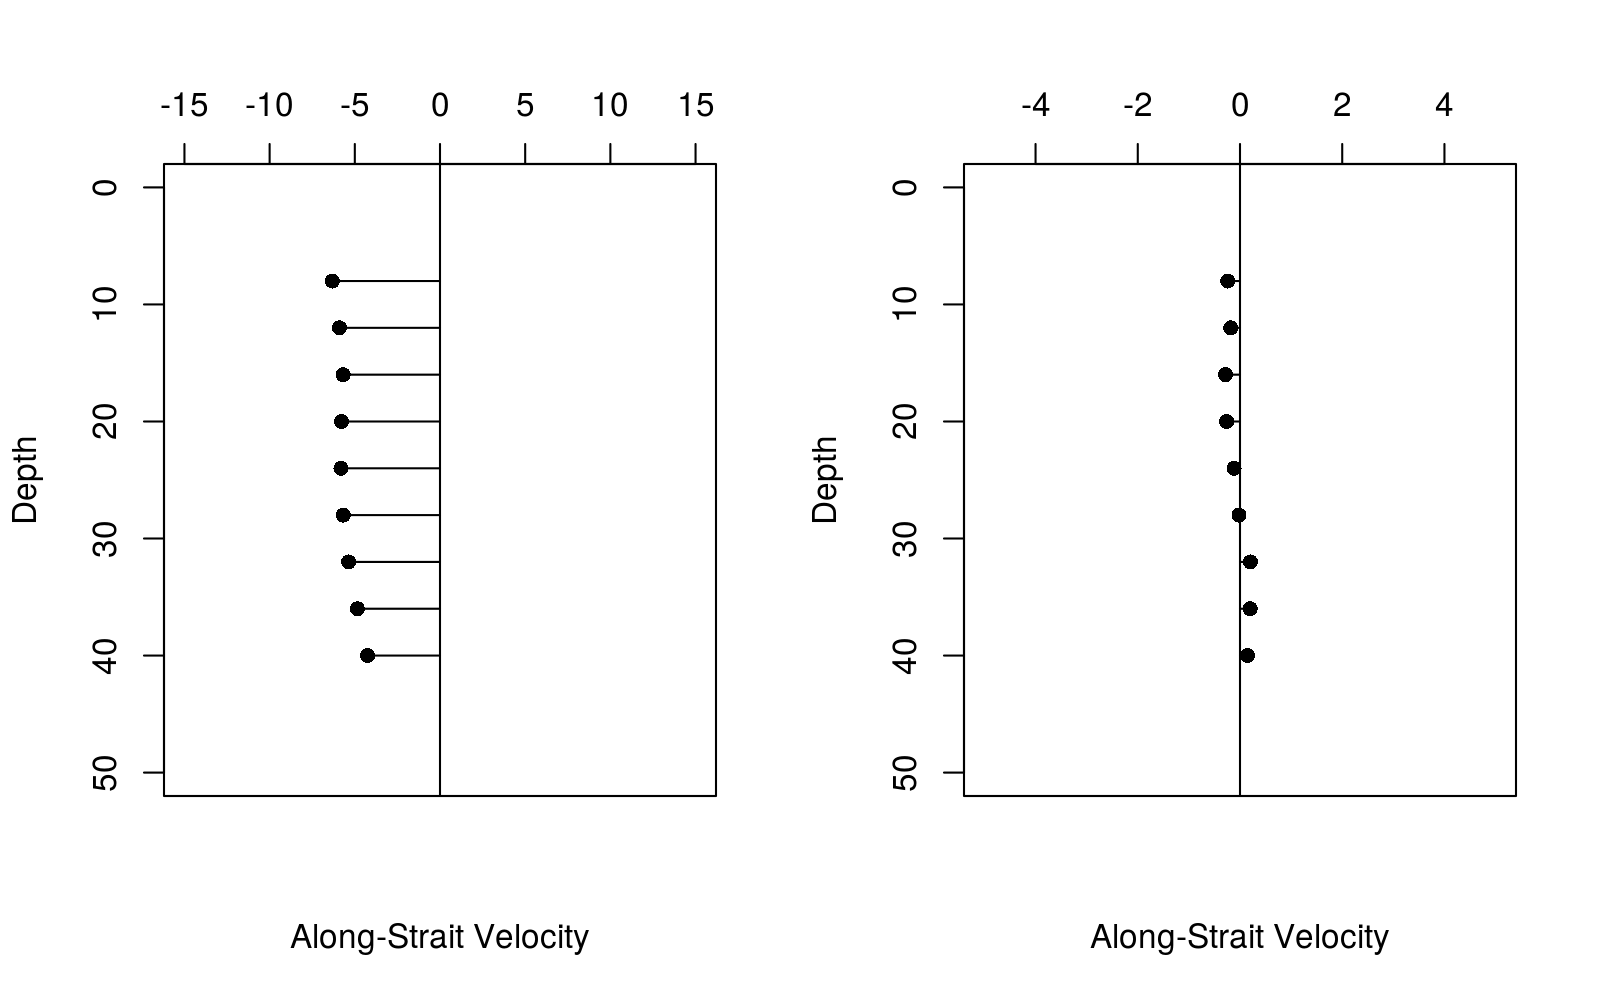
\includegraphics[width = 0.8\textwidth]{./figures/44_smf_spring_2015.png}
\caption[Mean flow, Spring, 2015]{Mean flow, Spring: April 2015 - June 2015}
\label{f:smf_s_2015}
\end{figure}

\begin{figure}  
\centering
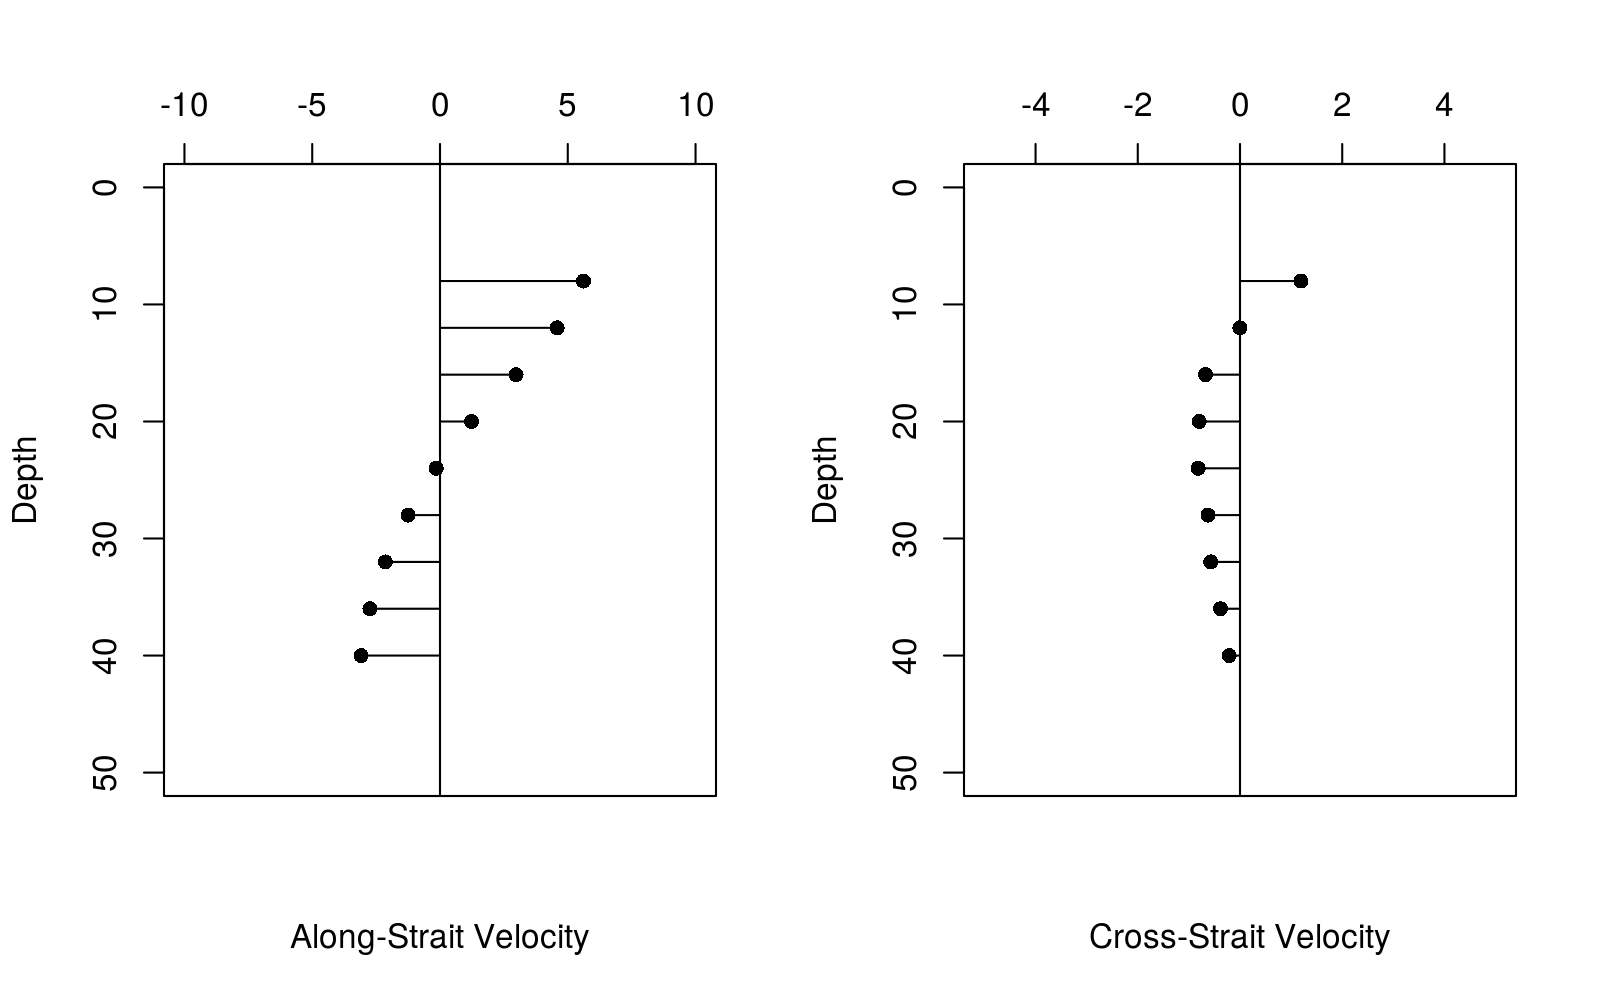
\includegraphics[width = 0.8\textwidth]{./figures/45_smf_spring_2016.png}
\caption[Mean flow, Spring, 2016]{Mean flow, Spring: April 2016 - June 2016}
\label{f:smf_s_2016}
\end{figure}


\begin{figure}  
\centering
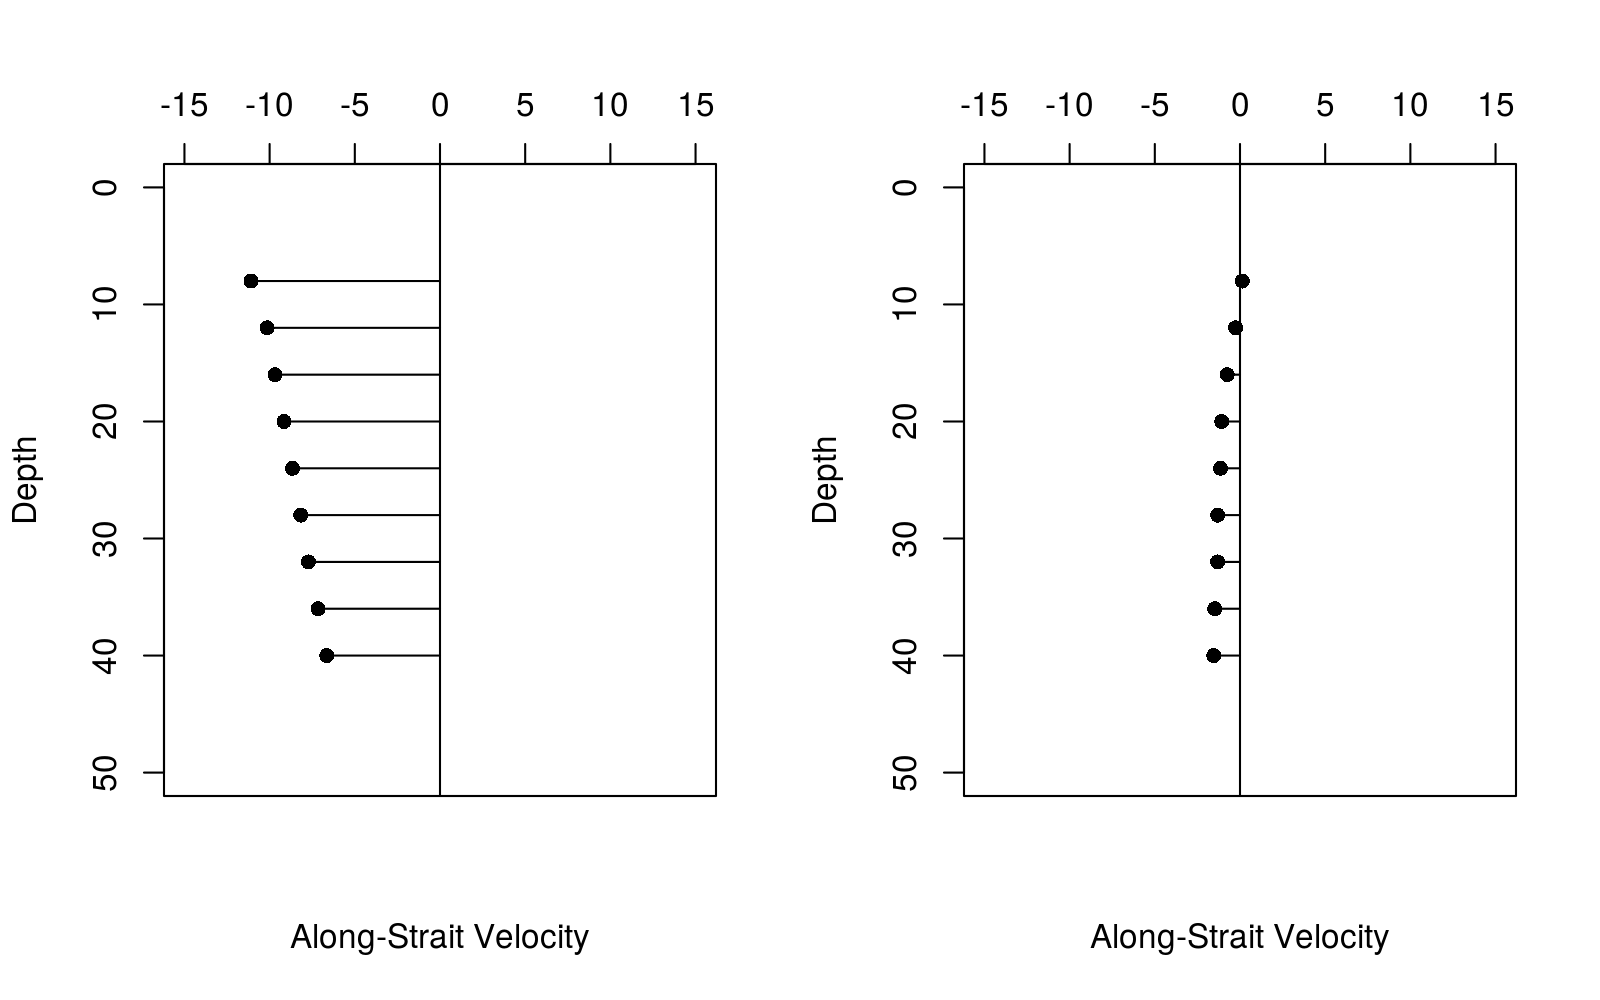
\includegraphics[width = 0.8\textwidth]{./figures/46_smf_earlySummer_2015.png}
\caption[Mean flow, Early Summer, 2015]{Mean flow, Early Summer: July 2015 - August 2015}
\label{f:smf_es_2015}
\end{figure}

\begin{figure}  
\centering
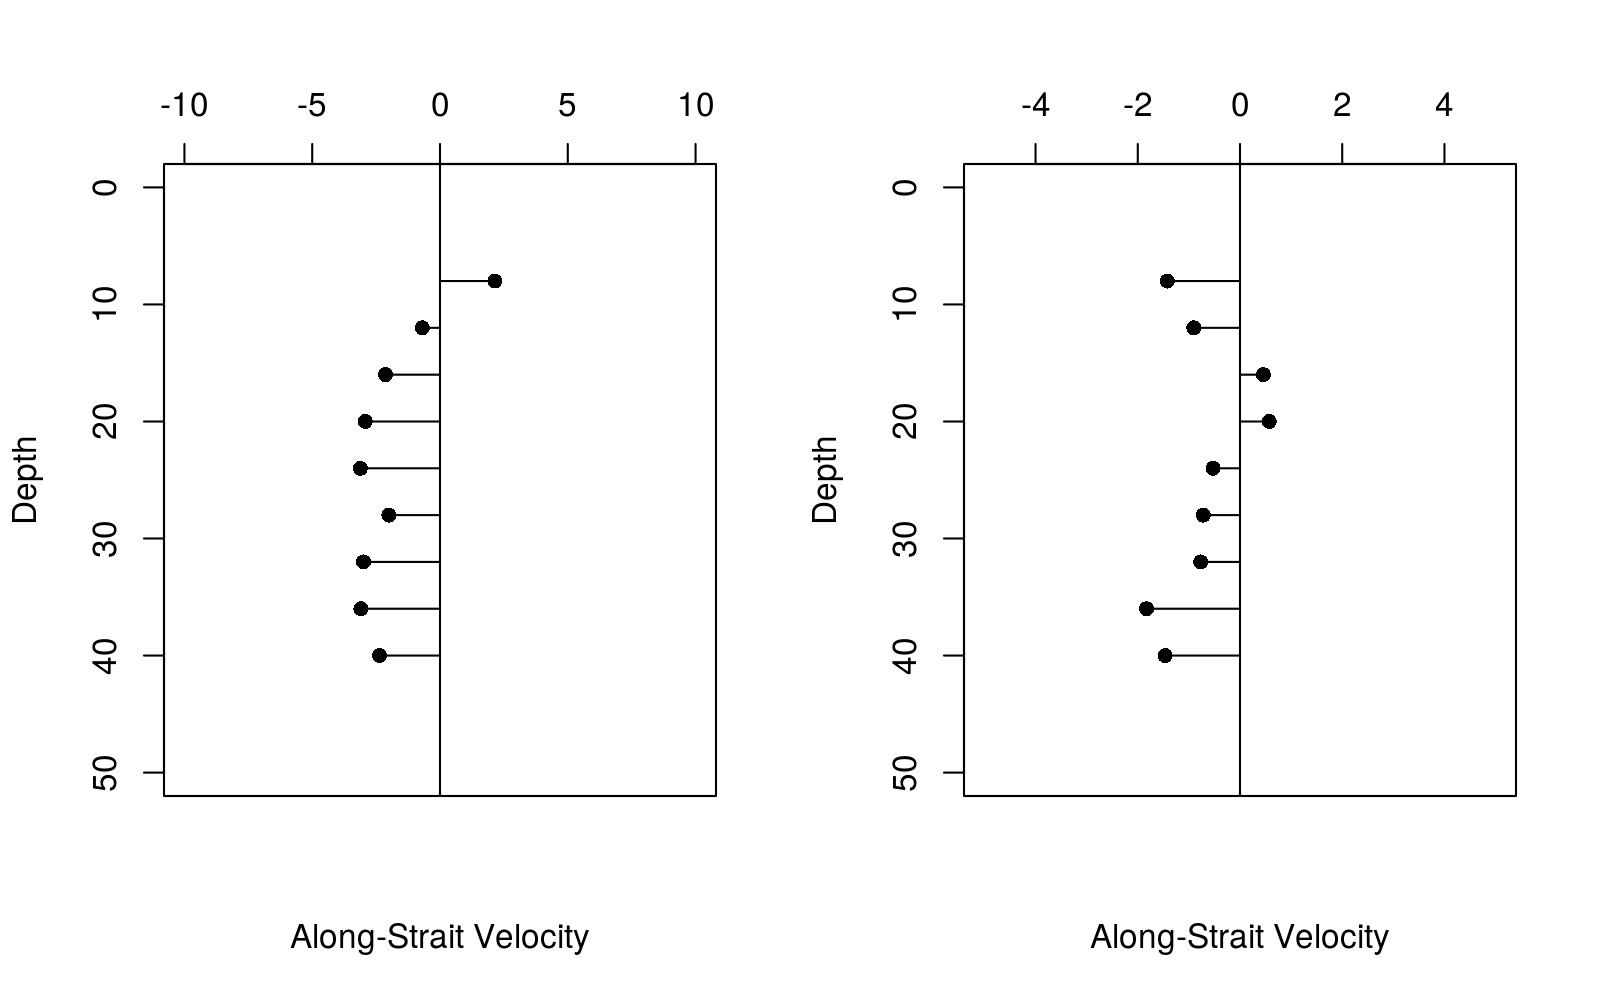
\includegraphics[width = 0.8\textwidth]{./figures/47_smf_earlySummer_2016.png}
\caption[Mean flow, Early Summer, 2016]{Mean flow, Early Summer: July 2016 - August 2016}
\label{f:smf_es_2016}
\end{figure}



\begin{figure}  
\centering
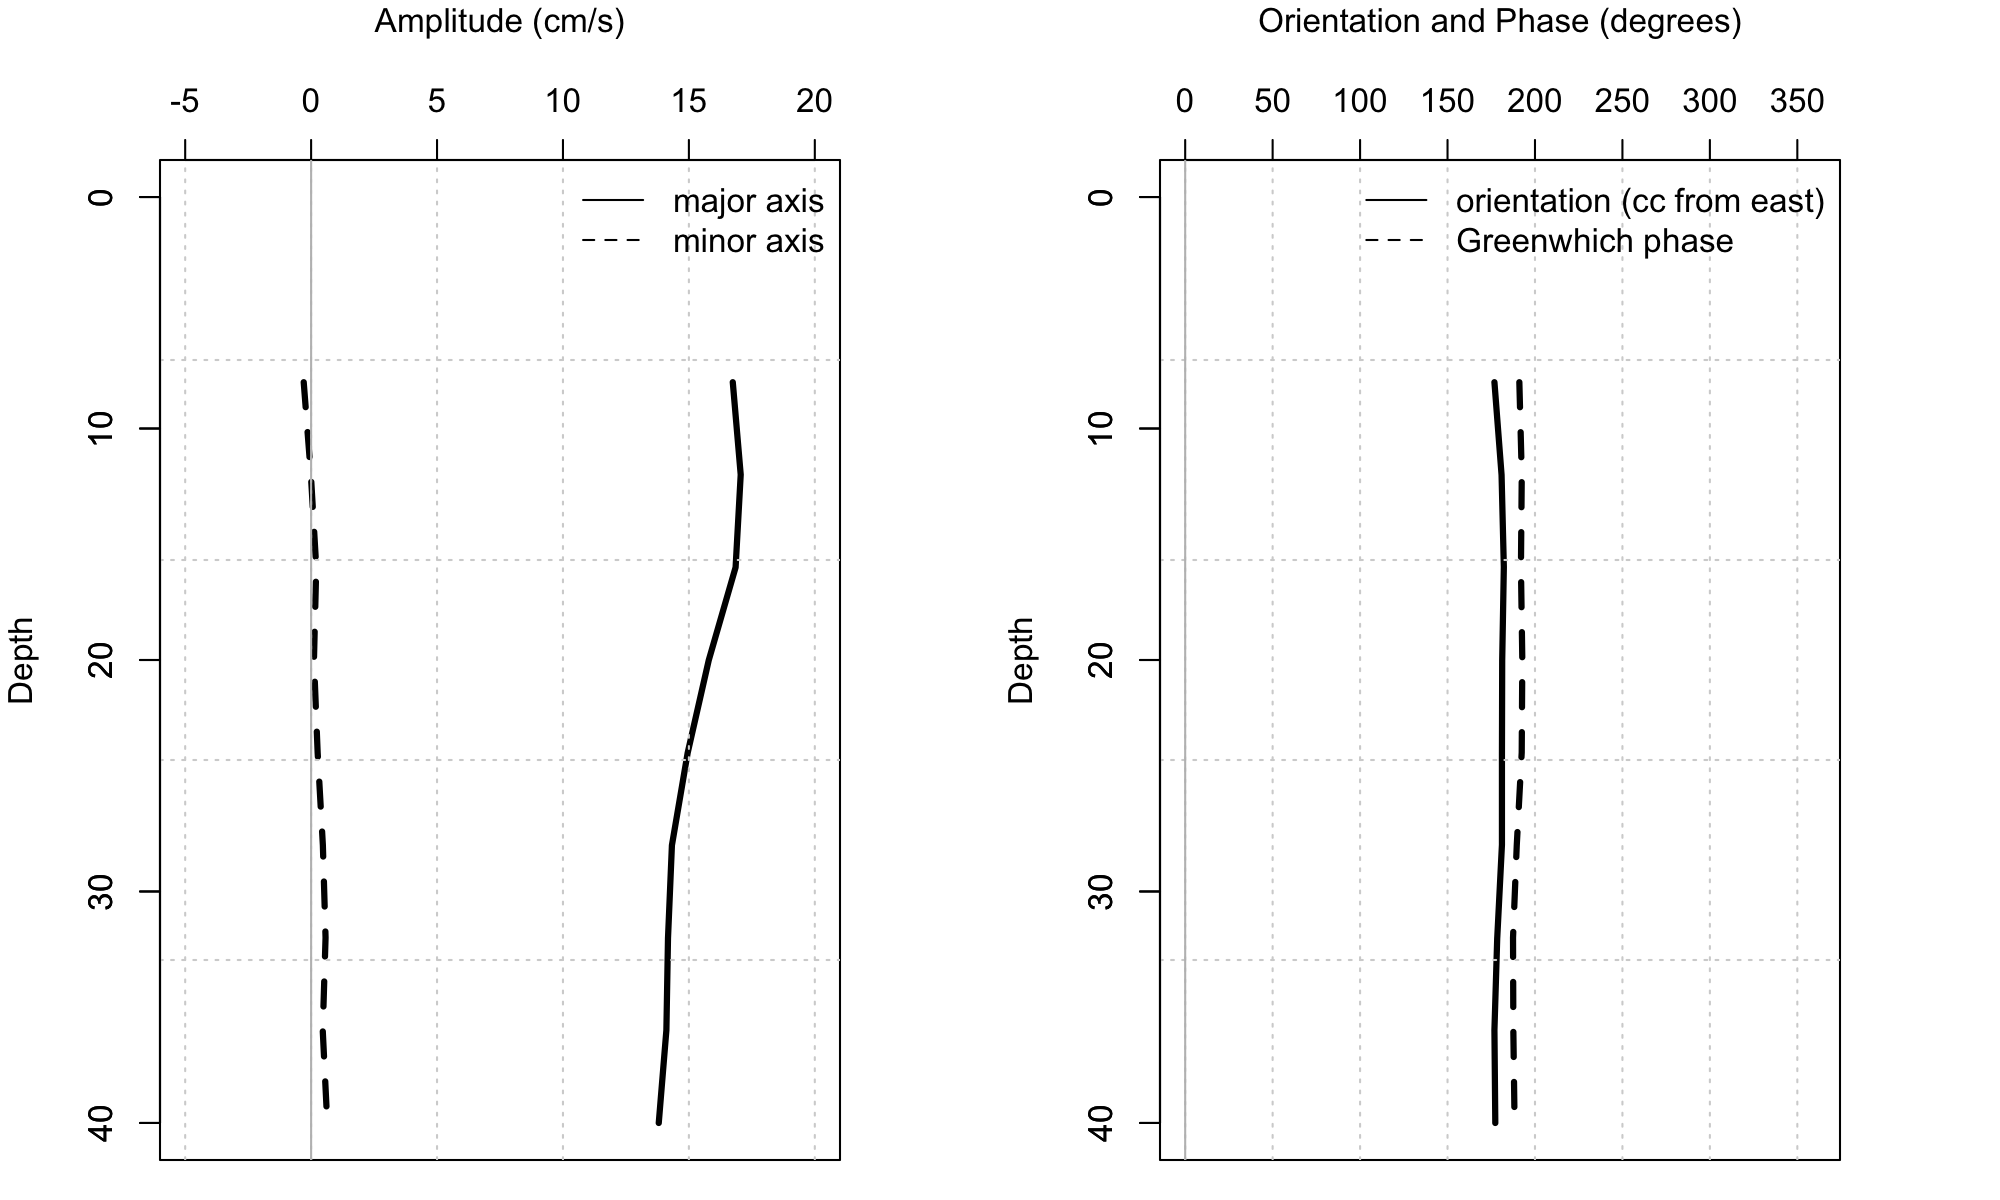
\includegraphics[width = 0.8\textwidth]{./figures/48_M2TC_if_2014.png}
  \caption[M2 Tidal Constituents, Ice free, 2014]{M2 Tidal Constituents, Ice Free Period (August 12 2014 - September 27 2014)}
\label{f:m2_if_2014}
\end{figure}

\begin{figure}  
\centering
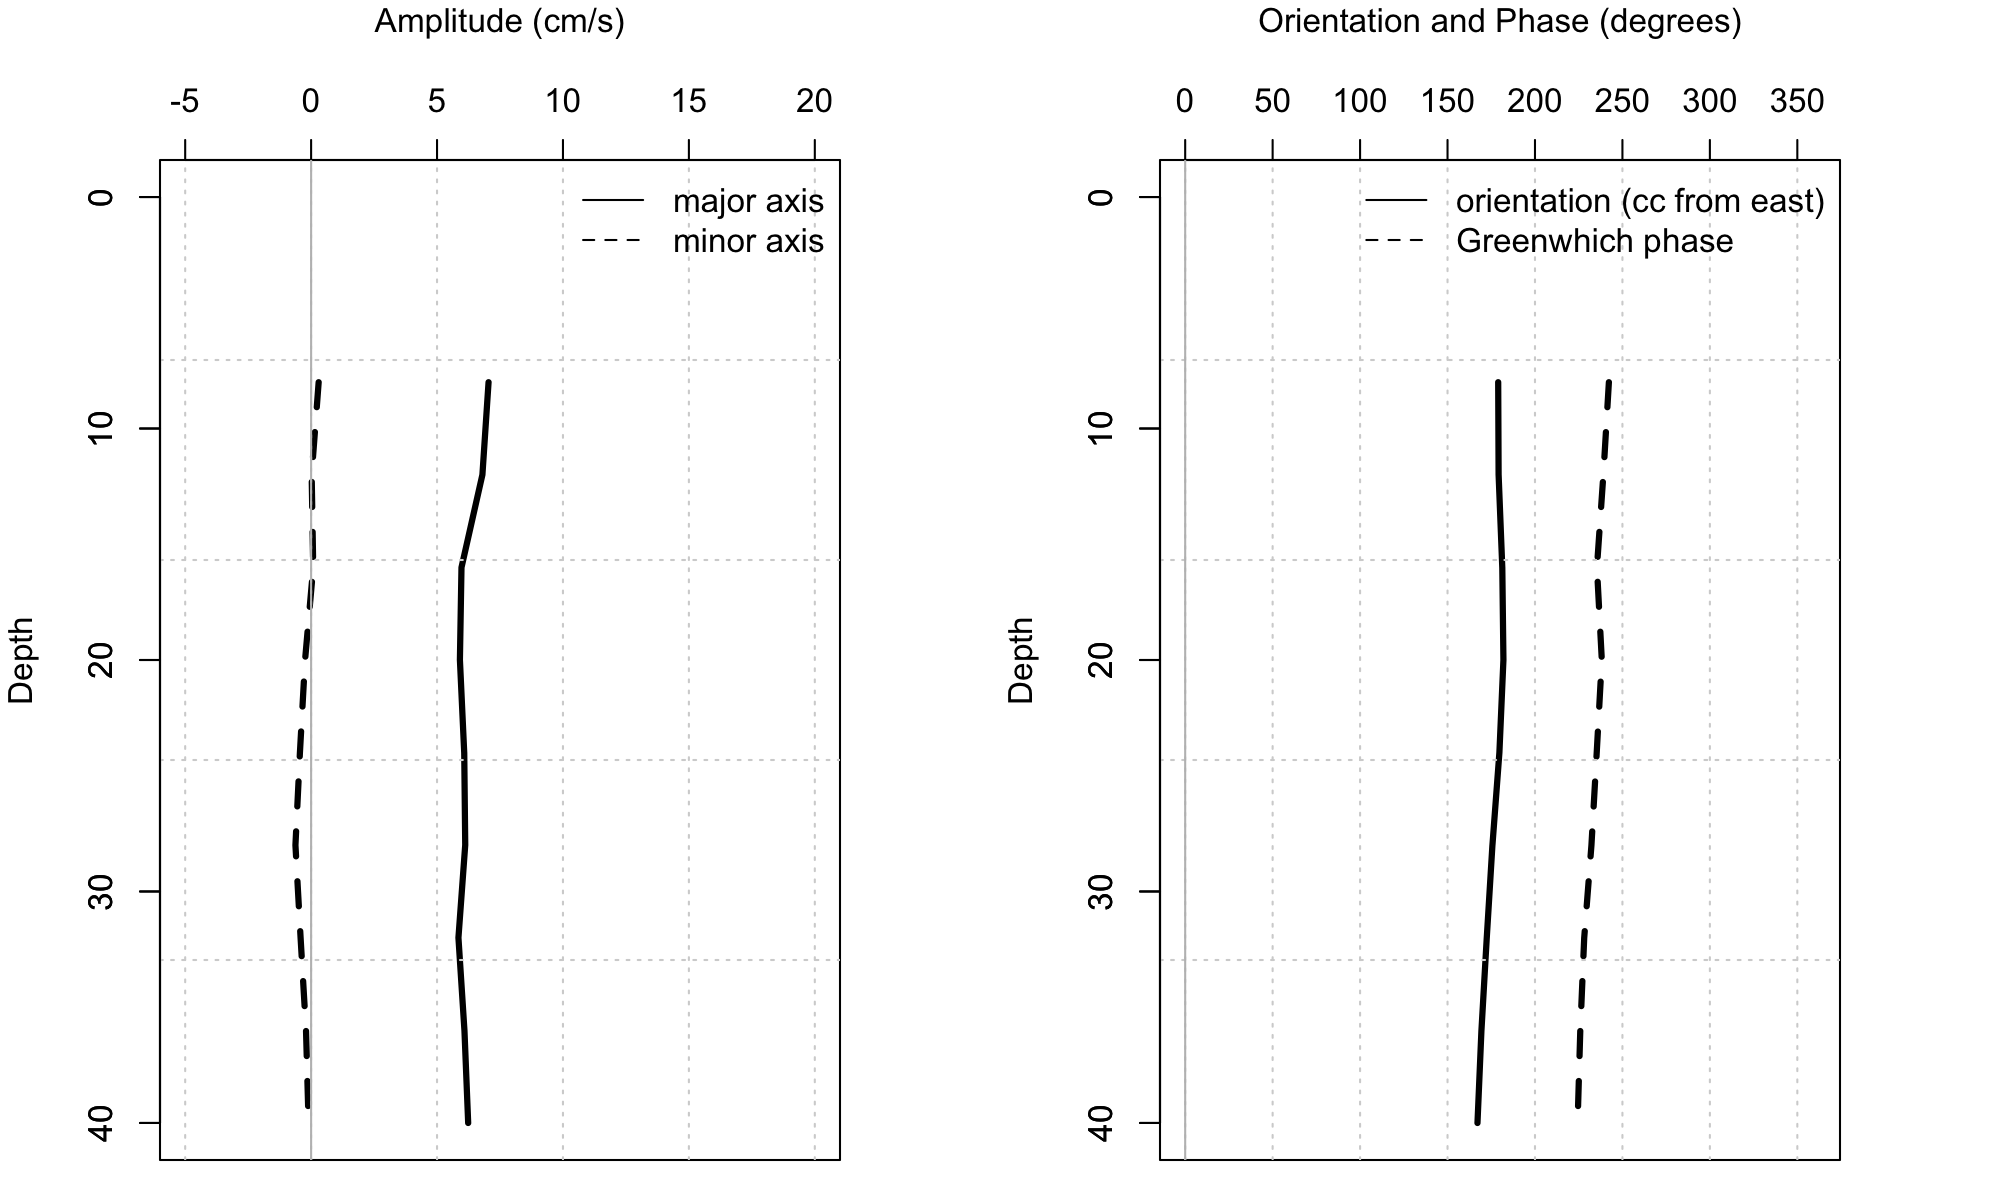
\includegraphics[width = 0.8\textwidth]{./figures/49_S2TC_if_2014.png}
\caption[S2 Tidal Constituents, Ice free, 2014]{S2 Tidal Constituents, Ice Free Period (August 12 2014 - September 27 2014)}
\label{f:s2_if_2014}
\end{figure}

\begin{figure}  
\centering
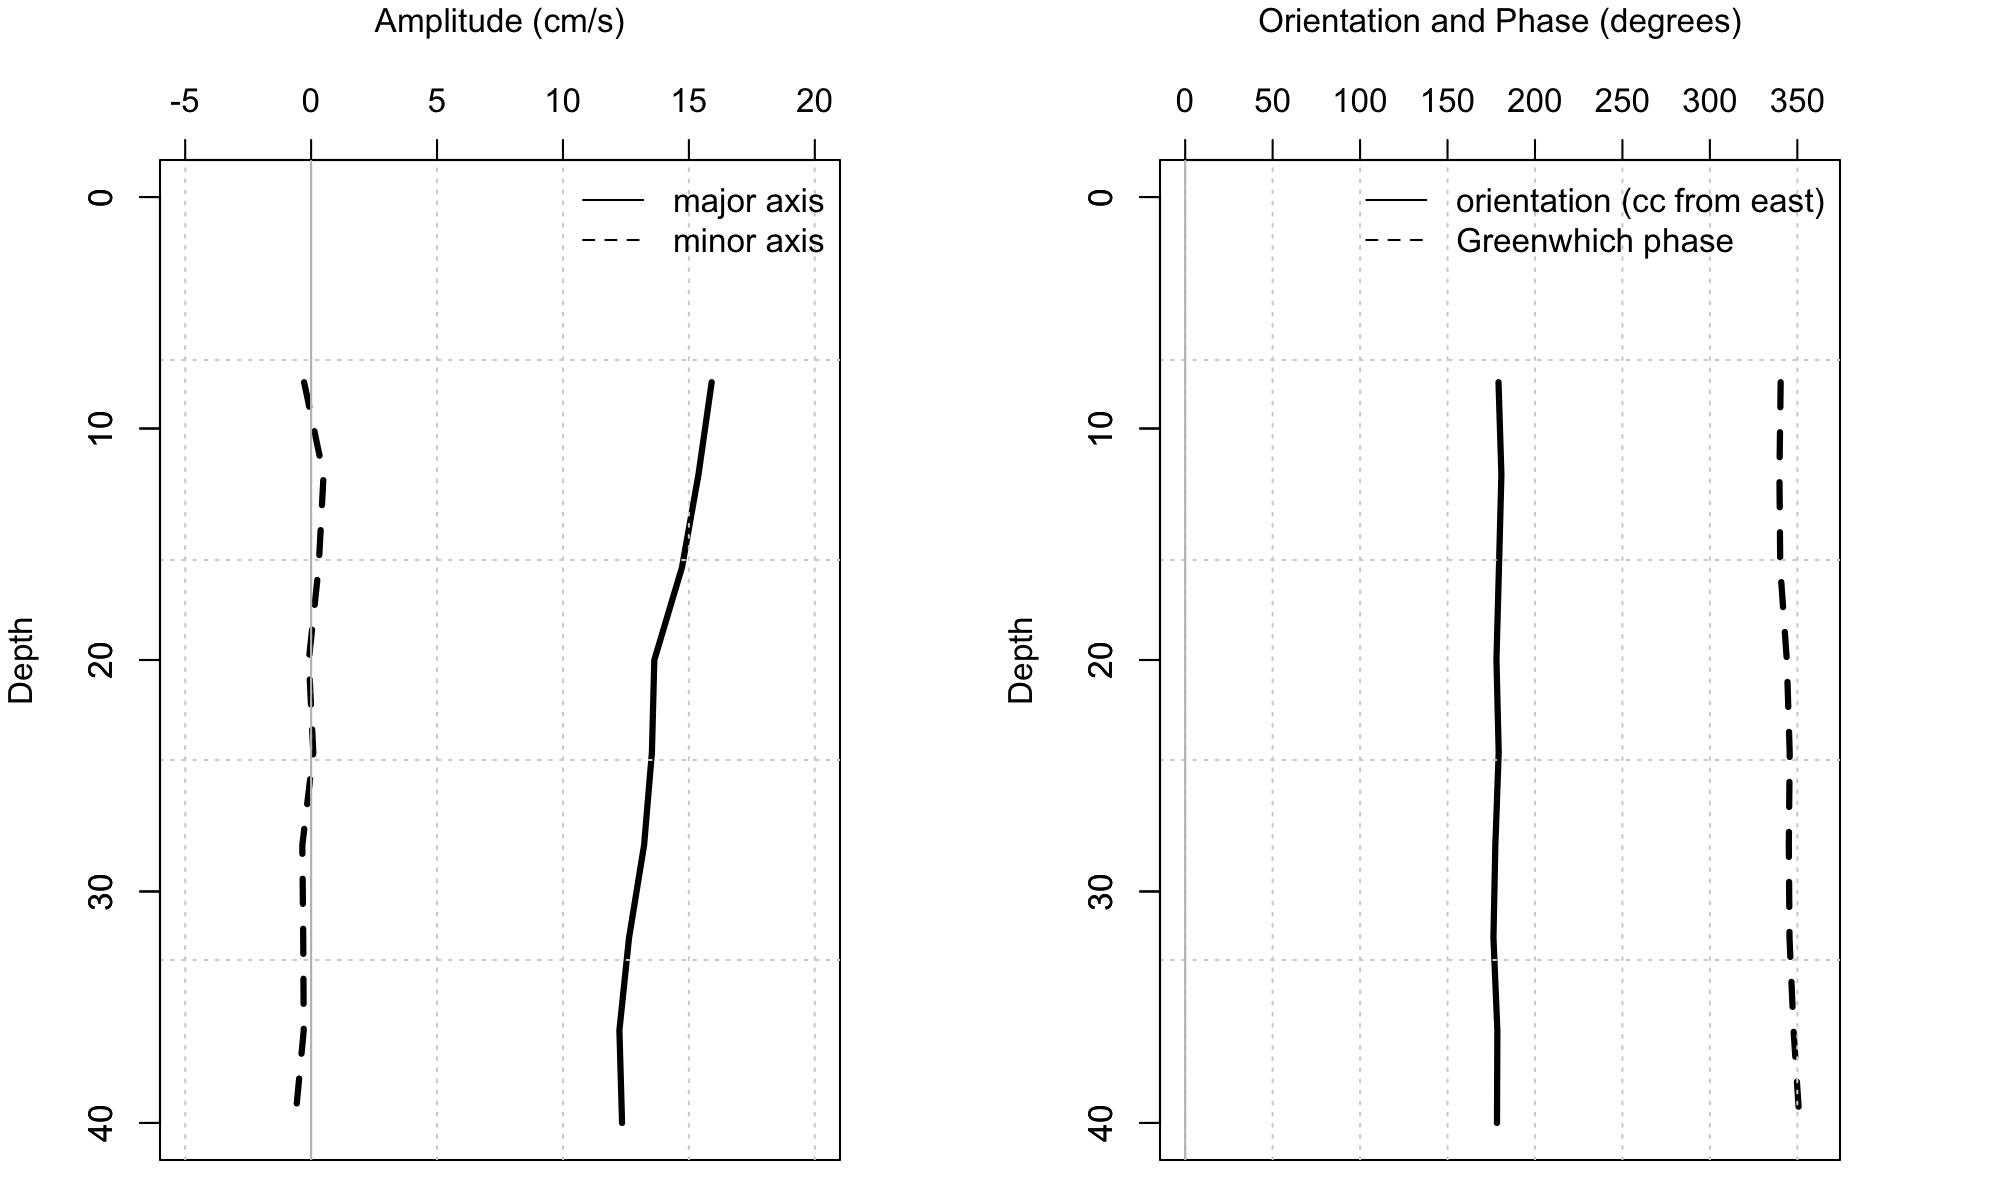
\includegraphics[width = 0.8\textwidth]{./figures/50_K1TC_if_2014.png}
\caption[K1 Tidal Constituents, Ice free, 2014]{K1 Tidal Constituents, Ice Free Period (August 12 2014 - September 27 2014)}
\label{f:k1_if_2014}
\end{figure}

\begin{figure}  
\centering
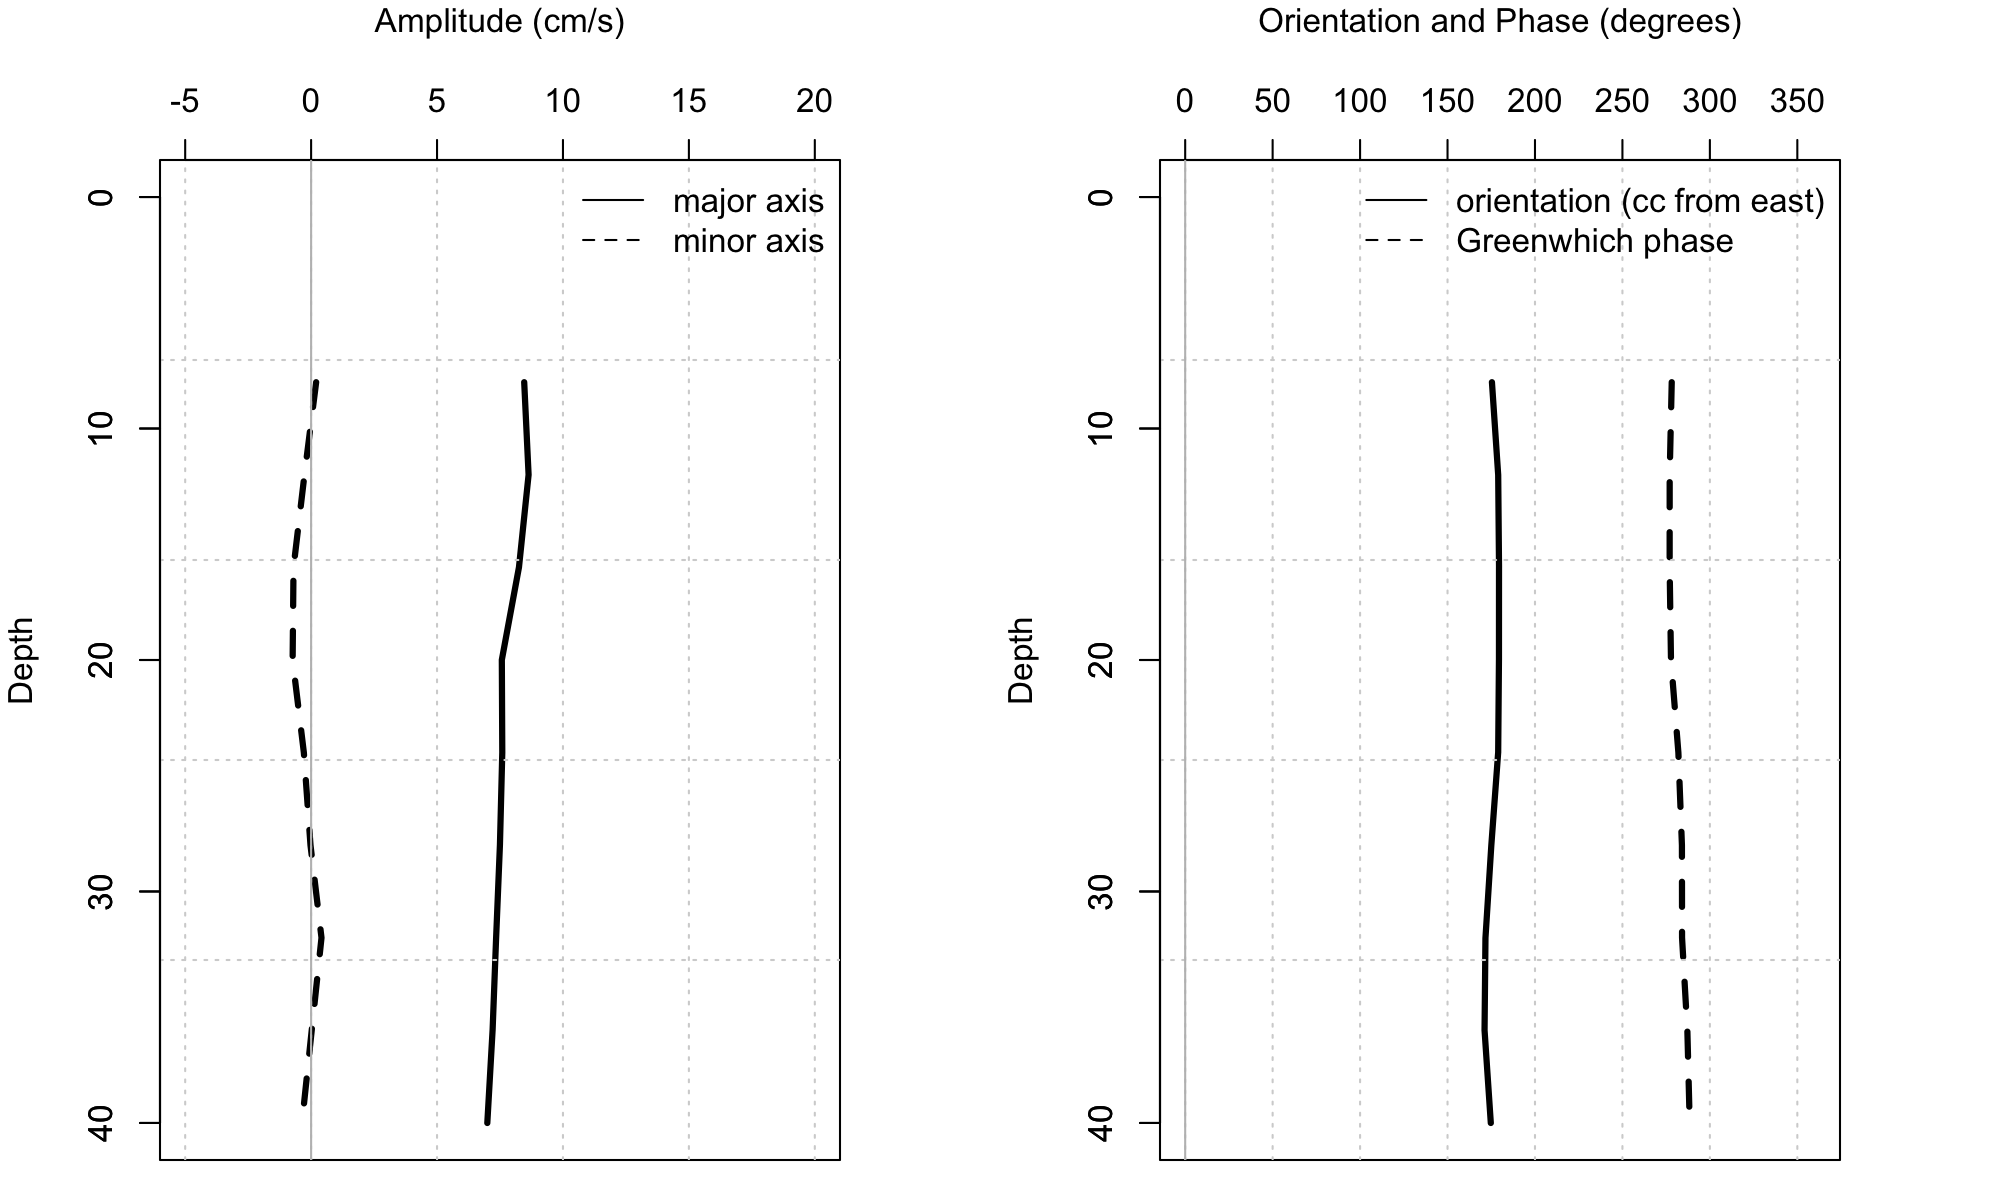
\includegraphics[width = 0.8\textwidth]{./figures/51_O1TC_if_2014.png}
\caption[O1 Tidal Constituents, Ice free, 2014]{O1 Tidal Constituents, Ice Free Period (August 12 2014 - September 27 2014)}
\label{f:o1_if_2014}
\end{figure}

\begin{figure}  
\centering
\includegraphics[width = 0.8\textwidth]{./figures/52_P1TC_if_2014.png}
\caption[P1 Tidal Constituents, Ice free, 2014]{P1 Tidal Constituents, Ice Free Period (August 12 2014 - September 27 2014)}
\label{f:p1_if_2014}
\end{figure}


\begin{figure}  
\centering
\includegraphics[width = 0.8\textwidth]{./figures/53_M2TC_if_2015.png}
\caption[M2 Tidal Constituents, Ice free, 2015]{M2 Tidal Constituents, Ice Free Period (July 15 2015 - September 27 2015)}
\label{f:m2_if_2015}
\end{figure}

\begin{figure}  
\centering
\includegraphics[width = 0.8\textwidth]{./figures/54_M2TC_si_2015.png}
\caption[M2 Tidal Constituents, Solid Ice, 2015]{M2 Tidal Constituents, Solid Ice Period (March 1 2016 - June 1 2016)}
\label{f:m2_si_2015}
\end{figure}


\begin{figure}  
\centering
\includegraphics[width = 0.8\textwidth]{./figures/55_S2TC_if_2015.png}
\caption[S2 Tidal Constituents, Ice free, 2015]{S2 Tidal Constituents, Ice Free Period (July 15 2015 - September 27 2015)}
\label{f:s2_if_2015}
\end{figure}

\begin{figure}  
\centering
\includegraphics[width = 0.8\textwidth]{./figures/56_S2TC_si_2015.png}
\caption[S2 Tidal Constituents, Solid Ice, 2015]{S2 Tidal Constituents, Solid Ice Period (March 1 2016 - June 1 2016)}
\label{f:s2_si_2015}
\end{figure}


\begin{figure}  
\centering
\includegraphics[width = 0.8\textwidth]{./figures/57_K1TC_if_2015.png}
\caption[K1 Tidal Constituents, Ice free, 2015]{K1 Tidal Constituents, Ice Free Period (July 15 2015 - September 27 2015)}
\label{f:k1_if_2015}
\end{figure}

\begin{figure}  
\centering
\includegraphics[width = 0.8\textwidth]{./figures/58_K1TC_si_2015.png}
\caption[K1 Tidal Constituents, Solid Ice, 2015]{K1 Tidal Constituents, Solid Ice Period (March 1 2016 - June 1 2016)}
\label{f:k1_si_2015}
\end{figure}


\begin{figure}  
\centering
\includegraphics[width = 0.8\textwidth]{./figures/59_O1TC_if_2015.png}
\caption[O1 Tidal Constituents, Ice free, 2015]{O1 Tidal Constituents, Ice Free Period (July 15 2015 - September 27 2015)}
\label{f:o1_if_2015}
\end{figure}

\begin{figure}  
\centering
\includegraphics[width = 0.8\textwidth]{./figures/60_O1TC_si_2015.png}
\caption[O1 Tidal Constituents, Solid Ice, 2015]{O1 Tidal Constituents, Solid Ice Period (March 1 2016 - June 1 2016)}
\label{f:o1_si_2015}
\end{figure}


\begin{figure}  
\centering
\includegraphics[width = 0.8\textwidth]{./figures/61_P1TC_if_2015.png}
\caption[P1 Tidal Constituents, Ice free, 2015]{P1 Tidal Constituents, Ice Free Period (July 15 2015 - September 27 2015)}
\label{f:p1_if_2015}
\end{figure}

\begin{figure}  
\centering
\includegraphics[width = 0.8\textwidth]{./figures/62_P1TC_si_2015.png}
\caption[P1 Tidal Constituents, Solid Ice, 2015]{P1 Tidal Constituents, Solid Ice Period (March 1 2016 - June 1 2016)}
\label{f:p1_si_2015}
\end{figure}



\begin{figure}  
\centering
\includegraphics[width = 0.8\textwidth]{./figures/63_iceDraft_2014_2015.png}
\caption[Ice Draft, 2014-2015]{Ice Draft: monthly time series, August 2014 - July 2015}
\label{f:id_2014_2015}
\end{figure}

\begin{figure}  
\centering
\includegraphics[width = 0.8\textwidth]{./figures/64_iceDraft_2015_2016.png}
\caption[Ice Draft, 2015-2016]{Ice Draft: monthly time series, August 2015 - July 2016}
\label{f:id_2015_2016}
\end{figure}




\begin{figure}  
\centering
\includegraphics[width = 0.8\textwidth]{./figures/65_iceHist_2014_2015.png}
\caption[Histograms of ice draft, 2014-2015]{Monthly Histograms of Ice Draft, August 2014 - August 2015}
\label{f:ih_2014_2015}
\end{figure}

\begin{figure}  
\centering
\includegraphics[width = 0.8\textwidth]{./figures/66_iceHist_2015_2016.png}
\caption[Histograms of ice draft, 2015-2016]{Monthly Histograms of Ice Draft, August 2015 - August 2016}
\label{f:ih_2015_2016}
\end{figure}



\begin{figure}  
\centering
\includegraphics[width = 0.8\textwidth]{./figures/67_iceDraftStat_2014_2015.png}
\caption[Ice draft Statistics, 2014-2015]{Ice Draft Statistics from Ice Profiling Sonar, August 2014 - July 2015}
\label{f:ids_2014_2015}
\end{figure}

\begin{figure}  
\centering
\includegraphics[width = 0.8\textwidth]{./figures/68_iceDraftStat_2015_2016.png}
\caption[Ice draft Statistics, 2015-2016]{Ice Draft Statistics from Ice Profiling Sonar, August 2015 - July 2016}
\label{f:ids_2015_2016}
\end{figure}
  


\begin{figure}  
\centering
\includegraphics[width = 0.8\textwidth]{./figures/69_iceVel_2014_2015.png}
\caption[Ice Velocity, 2014-2015]{Ice Velocity, August 2014 - August 2015}
\label{f:ivel_2014_2015}
\end{figure}

\begin{figure}  
\centering
\includegraphics[width = 0.8\textwidth]{./figures/70_iceVel_2015_2016.png}
\caption[Ice Velocity, 2015-2016]{Ice Velocity, August 2015 - August 2016}
\label{f:ivel_2015_2016}
\end{figure}



% latex table generated in R 3.6.1 by xtable 1.8-4 package
\begin{landscape}

\begin{table}[ht]
\centering
\caption[Mooring and Instrument Summary, 2011-2016]{Mooring and Instrument Summary, 2011-2016.} 
\label{t:mooringSummary}
\begin{tabular}{p{0.3in}p{.7in}p{.7in}p{.7in}p{.7in}p{.7in}p{.7in}p{.7in}p{.7in}p{.7in}p{.7in}p{.7in}}
 Year & BIO Consecutive Mooring Number & Mooring Name & Instrument Type & Serial Number & Moored Depth (m) & Sounding (m) & Latitude ($^\circ$ N) & Longitude ($^\circ$ W) & Start Date-Time (UTC) & End Date-Time (UTC) & Sampling Interval (Seconds) \\ 
\hline
2011 & 1801 & Hub & CTD & 361 & 121 & 122 & 74.62443 & -91.29958 & 2011-08-09 & 2012-09-01 & 3600 \\ 
2011 & 1802 & ADCP node & CTD & 374 & 63 & 135 & 74.623 & -91.2976 & 2011-08-10 & 2012-08-30 & 7200 \\ 
2011 & 1802 & ADCP node & CTD & 287 & 43 & 135 & 74.623 & -91.2976 & 2011-08-10 & 2012-08-30 & 3600 \\ 
2011 & 1802 & ADCP node & ADCP & 499 & 61 & 135 & 74.623 & -91.2976 & 2011-08-10 & 2011-08-16 & 7200 \\ 
2011 & 1802 & ADCP node & PoCo & 144 & 61 & 135 & 74.623 & -91.2976 & NA & NA & 7200 \\ 
2012 & 1825 & Hub & CTD & 864 & 156 & 151 & 74.608 & -91.2498 & 2012-09-03 & 2014-08-10 & 3600 \\ 
2012 & 1826 & ADCP node & CTD & 861 & 82 & 163 & 74.6061 & -91.2436 & 2012-09-03 18:00 & 2014-08-08 20:00 & 3600 \\ 
2012 & 1826 & ADCP node & CTD & 720 & 41 & 163 & 74.6061 & -91.2436 & 2012-09-03 17:30 & 2014-08-08 19:30 & 7200 \\
2012 & 1826 & ADCP node & ADCP & 1266 & 31 & 163 & 74.6061 & -91.2436 & 2012-09-03 17:30 & 2012-09-12 17:30 & 7200 \\ 
2012 & 1826 & ADCP node & PoCo & 146 & 31 & 163 & 74.6061 & -91.2436 & NA & NA & 7200 \\ 
2014 & 1877 & Hub & CTD & 7375 & 156 & NA & 74.6044 & -91.2453 & 2014-08-10 18:00 & 2016-08-09 16:00 & 7200 \\ 
2014 & 1878 & ADCP node & CTD & 11719 & 81 & 154 & 74.6045 & -91.2564 & 2014-08-12 16:00 & 2016-08-08 18:00 & 7200 \\ 
2014 & 1878 & ADCP node & CTD-ODO & 10513 & 47 & 154 & 74.6045 & -91.2564 & 2014-08-12 16:00 & 2016-08-08 18:01 & 7200 \\ 
2014 & 1878 & ADCP node & ADCP & 2456 & 40 & 154 & 74.6045 & -91.2564 & 2014-08-12 16:00 & 2016-07-02 16:00 & 7200 \\ 
2014 & 1878 & ADCP node & PoCo & 145 & 40 & 154 & 74.6045 & -91.2564 & NA & NA & 7200 \\ 
2014 & 1879 & IPS node & CTD-ODO & 10514 & 35 & 151 & 74.6022 & -91.2367 & 2014-08-12 14:00 & 2016-08-08 16:01 & 7200 \\ 
2014 & 1879 & IPS node & IPS & 51061 & 40 & 151 & 74.6022 & -91.2367 & 2014-08-12 23:00:18 & 2016-08-08 17:25:18 & 3 \\ 
\hline
\end{tabular}
\end{table}

% \begin{table}[ht]
% \centering
% \caption[Microcat/ADCP statistical summary, 2011-2012]{Microcat/ADCP statistical summary, 2011-2012.} 
% \label{t:ss_2011_2012}
% \begin{tabular}{p{0.3in}p{0.3in}p{.3in}p{.3in}p{.3in}p{.3in}p{.2in}p{.2in}p{.2in}p{.2in}p{.2in}p{.2in}p{.2in}p{.2in}p{.2in}p{.2in}p{.2in}p{.2in}p{.2in}p{.2in}p{.2in}p{.2in}p{.2in}p{.2in}p{.2in}p{.2in}}
% \multicolumn{2}{c}{Depth (m)} & \multicolumn{4}{c}{\textbf{Temperature ($^\circ$ C)}} & \multicolumn{4}{c}{\textbf{Salinity (psu)}} & \multicolumn{4}{c}{\textbf{Density (Sigma-T)}} & \multicolumn{4}{c}{\textbf{Along-Strait Velocity (cm/s)}} & \multicolumn{4}{c}{\textbf{Cross-Strait Velocity (cm/s)}}\\\hline
% CTD & ADCP & Avg & SD & Min & Max & Avg & SD & Min & Max & Avg & SD & Min & Max & Avg & SD & Min & Max & Avg & SD & Min & Max \\ 
% \hline
% x & x & x & x & x & x & x & x & x & x & x & x & x & x & x & x & x & x & x & x & x & x \\ 
% \hline  
% \end{tabular}
% \end{table}

\begin{table}[ht] 
\centering
\caption[Microcat CTD statistical summary, 2011-2012]{Microcat CTD statistical summary, 2011-2012.} 
\label{t:ss_2011_2012}
\begin{tabular}{c | c c c c | c c c c | c c c c}
\toprule 
\multicolumn{1}{c}{\textbf{Depth (m)}} & \multicolumn{4}{c}{\textbf{Temperature ($^\circ$ C)}} & \multicolumn{4}{c}{\textbf{Salinity (psu)}} & \multicolumn{4}{c}{\textbf{Density (Sigma-T)}} \\\hline
\midrule
CTD & Avg & SD & Min & Max & Avg & SD & Min & Max & Avg & SD & Min & Max \\  
\midrule 
\multicolumn{13}{l}{Annual} \\
\midrule
41 & -1.23 & 1.01 & -1.78 & 5.35 & 32.18 & 0.41 & 29.95 & 32.9 & 25.87 & 0.36 & 23.94 & 26.47 \\
61 & -1.39 & 0.56 & -1.77 & 3.18 & 32.34 & 0.32 & 31.1 & 32.94 & 26.01 & 0.27 & 24.99 & 26.49 \\
155 & -1.29 & 0.21 & -1.77 & 0.89 & 32.68 & 0.24 & 31.47 & 33.47 & 26.28 & 0.2 & 25.22 & 26.91 \\
\midrule 
\multicolumn{13}{l}{Fall (August - December)} \\
\midrule
41 & -0.55 & 1.35 & -1.77 & 5.35 & 31.79 & 0.37 & 30.86 & 32.77 & 25.52 & 0.32 & 24.47 & 26.33 \\
61 & -0.94 & 0.7 & -1.77 & 3.18 & 32.08 & 0.39 & 31.1 & 32.88 & 25.78 & 0.33 & 24.99 & 26.44 \\
155 & -1.21 & 0.25 & -1.73 & 0.89 & 32.67 & 0.28 & 31.47 & 33.47 & 26.27 & 0.23 & 25.22 & 26.91 \\
\midrule  
\multicolumn{13}{l}{Winter/Spring (January - June)} \\
\midrule
41 & -1.74 & 0.03 & -1.78 & -1.55 & 32.45 & 0.08 & 32.18 & 32.66 & 26.11 & 0.07 & 25.89 & 26.27 \\
61 & -1.72 & 0.05 & -1.77 & -1.4 & 32.48 & 0.08 & 32.2 & 32.75 & 26.13 & 0.07 & 25.9 & 26.35 \\
155 & -1.37 & 0.17 & -1.77 & -1 & 32.7 & 0.12 & 32.21 & 33.05 & 26.3 & 0.1 & 25.91 & 26.58 \\
\bottomrule
\end{tabular}
\end{table}


\begin{table}[ht] 
\centering
\caption[Microcat CTD statistical summary, 2012-2013]{Microcat CTD statistical summary, 2012-2013.} 
\label{t:ss_2012_2013}
\begin{tabular}{c | c c c c | c c c c | c c c c}
\toprule 
\multicolumn{1}{c}{\textbf{Depth (m)}} & \multicolumn{4}{c}{\textbf{Temperature ($^\circ$ C)}} & \multicolumn{4}{c}{\textbf{Salinity (psu)}} & \multicolumn{4}{c}{\textbf{Density (Sigma-T)}} \\\hline
\midrule
CTD & Avg & SD & Min & Max & Avg & SD & Min & Max & Avg & SD & Min & Max \\  
\midrule 
\multicolumn{13}{l}{Annual} \\
\midrule
41 & -1.37 & 0.4 & -1.75 & 0.92 & 31.99 & 0.37 & 30.18 & 32.69 & 25.72 & 0.31 & 24.17 & 26.29 \\
82 & -1.24 & 0.12 & -1.72 & -0.18 & 32.65 & 0.23 & 31.55 & 33.18 & 26.25 & 0.19 & 25.35 & 26.68 \\
156 & -0.93 & 0.19 & -1.35 & -0.26 & 33.23 & 0.18 & 32.32 & 33.65 & 26.71 & 0.14 & 25.99 & 27.03 \\
\midrule 
\multicolumn{13}{l}{Fall (August - December)} \\
\midrule
41 & -1.03 & 0.5 & -1.71 & 0.92 & 31.69 & 0.38 & 30.18 & 32.5 & 25.47 & 0.32 & 24.17 & 26.14 \\
82 & -1.2 & 0.13 & -1.49 & -0.18 & 32.45 & 0.2 & 31.55 & 33.03 & 26.09 & 0.16 & 25.35 & 26.56 \\
156 & -0.97 & 0.17 & -1.35 & -0.48 & 33.17 & 0.23 & 32.32 & 33.63 & 26.67 & 0.18 & 25.99 & 27.0 \\
\midrule  
\multicolumn{13}{l}{Winter/Spring (January - June)} \\
\midrule
41 & -1.59 & 0.12 & -1.75 & -1.2 & 32.1 & 0.24 & 31.55 & 32.63 & 25.82 & 0.2 & 25.38 & 26.24 \\
82 & -1.26 & 0.13 & -1.72 & -0.9 & 32.73 & 0.17 & 32.2 & 33.18 & 26.32 & 0.14 & 25.89 & 26.68 \\
156  & -0.92 & 0.18 & -1.25 & -0.28 & 33.25 & 0.13 & 32.77 & 33.61 & 26.73 & 0.1 & 26.35 & 26.99 \\
\bottomrule
\end{tabular}
\end{table}


\begin{table}[ht] 
\centering
\caption[Microcat CTD statistical summary, 2013-2014]{Microcat CTD statistical summary, 2013-2014.} 
\label{t:ss_2013_2014}
\begin{tabular}{c | c c c c | c c c c | c c c c}
\toprule 
\multicolumn{1}{c}{\textbf{Depth (m)}} & \multicolumn{4}{c}{\textbf{Temperature ($^\circ$ C)}} & \multicolumn{4}{c}{\textbf{Salinity (psu)}} & \multicolumn{4}{c}{\textbf{Density (Sigma-T)}} \\\hline
\midrule
CTD & Avg & SD & Min & Max & Avg & SD & Min & Max & Avg & SD & Min & Max \\  
\midrule 
\multicolumn{13}{l}{Annual} \\
\midrule
41 & -1.5 & 0.25 & -1.78 & 0.34 & 32.31 & 0.3 & 31.38 & 32.94 & 25.99 & 0.25 & 25.24 & 26.5 \\
82 & -1.33 & 0.14 & -1.76 & -0.86 & 32.76 & 0.23 & 31.8 & 33.26 & 26.35 & 0.19 & 25.57 & 26.75 \\
156 & -0.99 & 0.18 & -1.48 & -0.4 & 33.2 & 0.16 & 32.42 & 33.6 & 26.7 & 0.13 & 26.06 & 27 \\
\midrule 
\multicolumn{13}{l}{Fall (August - December)} \\
\midrule
41 & -1.39 & 0.29 & -1.77 & -0.28 & 32.13 & 0.31 & 31.38 & 32.75 & 25.84 & 0.25 & 25.24 & 26.34 \\
82 & -1.23 & 0.11 & -1.73 & -0.86 & 32.56 & 0.21 & 31.8 & 33.1 & 26.18 & 0.17 & 25.57 & 26.62 \\
156 & -0.96 & 0.17 & -1.25 & -0.4 & 33.13 & 0.21 & 32.42 & 33.6 & 26.63 & 0.17 & 26.06 & 27 \\
\midrule  
\multicolumn{13}{l}{Winter/Spring (January - June)} \\
\midrule
41 & -1.63 & 0.09 & -1.78 & -1.36 & 32.48 & 0.21 & 31.78 & 32.94 & 26.13 & 0.17 & 25.56 & 26.5 \\
82 & -1.39 & 0.12 & -1.76 & -1.08 & 32.9 & 0.14 & 32.51 & 33.26 & 26.46 & 0.11 & 26.15 & 26.75 \\
156 & -1.03 & 0.19 & -1.48 & -0.46 & 33.24 & 0.1 & 32.79 & 33.54 & 26.73 & 0.08 & 26.38 & 26.95 \\
\bottomrule
\end{tabular}
\end{table}


\begin{table}[ht] 
\centering
\caption[Microcat CTD statistical summary, 2014-2015]{Microcat CTD statistical summary, 2014-2015.} 
\label{t:ss_2014_2015}
\begin{tabular}{c | c c c c | c c c c | c c c c | c c c c}
\toprule 
\multicolumn{1}{c}{\textbf{Depth (m)}} & \multicolumn{4}{c}{\textbf{Temperature ($^\circ$ C)}} & \multicolumn{4}{c}{\textbf{Salinity (psu)}} & \multicolumn{4}{c}{\textbf{Density (Sigma-T)}} & \multicolumn{4}{c}{\textbf{Oxygen (ml/l)}} \\\hline
\midrule
CTD & Avg & SD & Min & Max & Avg & SD & Min & Max & Avg & SD & Min & Max & Avg & SD & Min & Max \\  
\midrule 
\multicolumn{17}{l}{Annual} \\
\midrule
35 & -1.16 & 1 & -1.81 & 3.67 & 32.35 & 0.47 & 31.05 & 33.04 & 26.01 & 0.41 & 24.67 & 26.59 & 7.23 & 0.56 & 5.96 & 9.41 \\
47 & -1.28 & 0.72 & -1.8 & 3.35 & 32.5 & 0.39 & 31.19 & 33.04 & 26.13 & 0.34 & 24.82 & 26.59 & 7 & 0.47 & 5.8 & 9.1 \\
81 & -1.41 & 0.2 & -1.8 & -0.24 & 32.79 & 0.21 & 31.76 & 33.45 & 26.37 & 0.17 & 25.54 & 26.9 & NA & NA & Inf & -Inf \\
156 & -0.99 & 0.21 & -1.69 & -0.07 & 33.29 & 0.2 & 32.57 & 33.79 & 26.77 & 0.15 & 26.19 & 27.13 & NA & NA & Inf & -Inf \\
\midrule 
\multicolumn{17}{l}{Fall (August - December)} \\
\midrule
35 & -1.37 & 0.29 & -1.77 & 0.04 & 32.07 & 0.32 & 31.08 & 32.66 & 25.79 & 0.26 & 24.99 & 26.27 & 7.35 & 0.33 & 6.46 & 8.63 \\
47 & -1.32 & 0.26 & -1.77 & -0.13 & 32.25 & 0.28 & 31.33 & 32.72 & 25.94 & 0.23 & 25.17 & 26.32 & 7.03 & 0.33 & 6.38 & 8.08 \\
81 & -1.28 & 0.11 & -1.56 & -0.83 & 32.61 & 0.18 & 31.76 & 33.05 & 26.22 & 0.15 & 25.54 & 26.58 & NA & NA & Inf & -Inf \\
156 & -0.96 & 0.19 & -1.36 & -0.41 & 33.23 & 0.23 & 32.57 & 33.66 & 26.72 & 0.18 & 26.19 & 27.05 & NA & NA & Inf & -Inf \\
\midrule  
\multicolumn{17}{l}{Winter/Spring (January - June)} \\
\midrule
35 & -1.58 & 0.33 & -1.81 & 0.95 & 32.73 & 0.21 & 31.81 & 33.04 & 26.33 & 0.18 & 25.53 & 26.59 & 6.94 & 0.49 & 5.96 & 9.41 \\ 
47 & -1.61 & 0.2 & -1.8 & 0.28 & 32.79 & 0.16 & 31.97 & 33.04 & 26.38 & 0.13 & 25.65 & 26.59 & 6.81 & 0.34 & 5.8 & 9.1 \\
81 & -1.55 & 0.16 & -1.8 & -0.93 & 32.92 & 0.13 & 32.63 & 33.45 & 26.48 & 0.1 & 26.25 & 26.9 & NA & NA & Inf & -Inf \\
156 & -1.03 & 0.23 & -1.69 & -0.07 & 33.34 & 0.17 & 32.66 & 33.79 & 26.81 & 0.13 & 26.27 & 27.13 & NA & NA & Inf & -Inf \\
\bottomrule
\end{tabular}
\end{table}


\begin{table}[ht] 
\centering
\caption[Microcat CTD statistical summary, 2015-2016]{Microcat CTD statistical summary, 2015-2016.} 
\label{t:ss_2015_2016}
\begin{tabular}{c | c c c c | c c c c | c c c c | c c c c}
\toprule 
\multicolumn{1}{c}{\textbf{Depth (m)}} & \multicolumn{4}{c}{\textbf{Temperature ($^\circ$ C)}} & \multicolumn{4}{c}{\textbf{Salinity (psu)}} & \multicolumn{4}{c}{\textbf{Density (Sigma-T)}} & \multicolumn{4}{c}{\textbf{Oxygen (ml/l)}} \\\hline
\midrule
CTD & Avg & SD & Min & Max & Avg & SD & Min & Max & Avg & SD & Min & Max & Avg & SD & Min & Max \\  
\midrule 
\multicolumn{17}{l}{Annual} \\
\midrule
35 & -1.22 & 0.83 & -1.79 & 2.57 & 32.3 & 0.4 & 30.61 & 33.03 & 25.97 & 0.35 & 24.48 & 26.57 & 7.37 & 0.47 & 6.13 & 8.72 \\
47 & -1.33 & 0.51 & -1.78 & 1.62 & 32.53 & 0.31 & 30.72 & 33.01 & 26.16 & 0.26 & 24.57 & 26.56 & 6.97 & 0.45 & 5.99 & 8.66 \\
81 & -1.29 & 0.15 & -1.79 & -0.72 & 32.94 & 0.22 & 31.97 & 33.43 & 26.49 & 0.18 & 25.71 & 26.89 & NA & NA & Inf & -Inf \\
156 & -0.9 & 0.2 & -1.33 & -0.3 & 33.28 & 0.19 & 32.56 & 33.68 & 26.75 & 0.15 & 26.18 & 27.05 & NA & NA & Inf & -Inf \\
\midrule 
\multicolumn{17}{l}{Fall (August - December)} \\
\midrule
35 & -0.85 & 0.88 & -1.75 & 2.57 & 32.12 & 0.32 & 30.62 & 32.8 & 25.81 & 0.27 & 24.58 & 26.38 & 7.37 & 0.37 & 6.37 & 8.48 \\
47 & -1.07 & 0.47 & -1.74 & 0.75 & 32.39 & 0.26 & 31.11 & 32.91 & 26.04 & 0.21 & 24.97 & 26.47 & 6.92 & 0.4 & 5.99 & 7.86 \\
81 & -1.21 & 0.14 & -1.73 & -0.72 & 32.78 & 0.24 & 31.97 & 33.22 & 26.36 & 0.19 & 25.71 & 26.71 & NA & NA & Inf & -Inf \\
156 & -0.9 & 0.2 & -1.33 & -0.34 & 33.18 & 0.21 & 32.56 & 33.61 & 26.67 & 0.16 & 26.18 & 27 & NA & NA & Inf & -Inf \\
\midrule  
\multicolumn{17}{l}{Winter/Spring (January - June)} \\
\midrule
35 & -1.69 & 0.1 & -1.79 & -1.19 & 32.52 & 0.15 & 32.08 & 32.91 & 26.16 & 0.12 & 25.81 & 26.47 & 7.32 & 0.49 & 6.13 & 8.54 \\
47 & -1.62 & 0.13 & -1.78 & -1.14 & 32.67 & 0.15 & 32.22 & 32.99 & 26.28 & 0.12 & 25.92 & 26.54 & 6.96 & 0.45 & 5.99 & 8.26 \\
81 & -1.34 & 0.15 & -1.79 & -0.98 & 33.03 & 0.14 & 32.63 & 33.43 & 26.57 & 0.11 & 26.25 & 26.89 & NA & NA & Inf & -Inf \\
156 & -0.89 & 0.21 & -1.27 & -0.3 & 33.35 & 0.13 & 32.78 & 33.68 & 26.81 & 0.1 & 26.36 & 27.05 & NA & NA & Inf & -Inf \\
\bottomrule
\end{tabular}
\end{table}


\end{landscape}


\begin{table}[ht]
\centering
\caption[Major Axis of Tidal Constituents]{Tidal Analysis: Major axis of each tidal constituent for ice-free and solid ice periods.} 
\label{t:majorAxis}
\begin{tabular}{| c | c | c c c c c |}
\hline
& Depth & M2 & S2 & K1 & O1 & P1 \\
\hline
& 8 & 0.17 & 0.07 & 0.16 & 0.08 & 0.01 \\
& 12 & 0.17 & 0.07 & 0.15 & 0.09 & 0.02 \\
& 16 & 0.17 & 0.06 & 0.15 & 0.08 & 0.02 \\
& 20 & 0.16 & 0.06 & 0.14 & 0.08 & 0.01 \\
2014, ice-free & 24 & 0.15 & 0.06 & 0.14 & 0.08 & 0.01 \\ 
(August 12 2014 - September 27 2014) & 28 & 0.14 & 0.06 & 0.13 & 0.07 & 0.01 \\
& 32 & 0.14 & 0.06 & 0.13 & 0.07 & 0.01 \\
& 36 & 0.14 & 0.06 & 0.12 & 0.07 & 0.01 \\
& 40 & 0.14 & 0.06 & 0.12 & 0.07 & 0.01 \\
 \hline
& 8 & 0.16 & 0.06 & 0.16 & 0.08 & 0.01 \\
& 12 & 0.16 & 0.06 & 0.15 & 0.08 & 0.01 \\
& 16 & 0.16 & 0.06 & 0.15 & 0.07 & 0.01 \\
& 20 & 0.15 & 0.06 & 0.15 & 0.07 & 0.01 \\
2015, ice-free & 24 & 0.15 & 0.06 & 0.15 & 0.07 & 0.01 \\
(July 15 2015 - September 27 2015) & 28 & 0.15 & 0.06 & 0.15 & 0.08 & 0 \\
& 32 & 0.15 & 0.06 & 0.15 & 0.08 & 0 \\
& 36 & 0.15 & 0.06 & 0.15 & 0.07 & 0 \\
& 40 & 0.14 & 0.06 & 0.15 & 0.08 & 0.01 \\
 \hline
& 8 & 0.11 & 0.04 & 0.11 & 0.06 & 0 \\
& 12 & 0.11 & 0.05 & 0.12 & 0.06 & 0 \\
& 16 & 0.12 & 0.05 & 0.12 & 0.06 & 0 \\
& 20 & 0.13 & 0.05 & 0.12 & 0.06 & 0 \\
2015, solid ice  & 24 & 0.13 & 0.05 & 0.12 & 0.06 & 0 \\
(March 1 2016 - June 1 2016) & 28 & 0.14 & 0.06 & 0.12 & 0.07 & 0.01 \\ 
& 32 & 0.14 & 0.06 & 0.12 & 0.07 & 0.01 \\
& 36 & 0.14 & 0.06 & 0.12 & 0.07 & 0.01 \\
& 40 & 0.14 & 0.06 & 0.12 & 0.07 & 0 \\
 \hline
\end{tabular}
\end{table}


\begin{table}[ht]
\centering
\caption[Minor Axis of Tidal Constituents]{Tidal Analysis: Minor axis of each tidal constituent for ice-free and solid ice periods.} 
\label{t:minorAxis}
\begin{tabular}{| c | c | c c c c c |}
\hline
& Depth & M2 & S2 & K1 & O1 & P1 \\
\hline
& 8 & 0 & 0 & 0 & 0 & 0 \\
& 12 & 0 & 0 & 0 & 0 & 0 \\
& 16 & 0 & 0 & 0 & -0.01 & 0 \\
& 20 & 0 & 0 & 0 & -0.01 & 0 \\
2014, ice-free & 24 & 0 & 0 & 0 & 0 & 0 \\
(August 12 2014 - September 27 2014) & 28 & 0 & -0.01 & 0 & 0 & 0 \\
& 32 & 0.01 & 0 & 0 & 0 & -0.01 \\
& 36 & 0 & 0 & 0 & 0 & -0.01 \\
& 40 & 0.01 & 0 & -0.01 & 0 & 0 \\
 \hline
& 8 & 0 & 0 & -0.01 & -0.01 & 0 \\
& 12 & 0 & -0.01 & -0.01 & 0 & 0.01 \\
& 16 & 0 & 0 & 0 & 0 & 0 \\
& 20 & 0 & 0 & 0 & 0 & 0 \\
2015, ice-free & 24 & 0.01 & 0 & 0 & 0 & 0 \\
(July 15 2015 - September 27 2015) & 28 & 0.01 & 0 & 0 & 0 & 0 \\
& 32 & 0.01 & 0 & 0 & 0 & 0 \\
& 36 & 0.01 & 0 & 0 & 0 & 0 \\
& 40 & 0.01 & 0 & 0 & 0 & 0 \\
 \hline
& 8 & 0.02 & 0.01 & 0 & 0 & 0  \\
& 12 & 0.02 & 0.01 & 0 & 0 & 0 \\
& 16 & 0.02 & 0.01 & 0 & 0 & 0 \\
& 20 & 0.01 & 0 & 0 & 0 & 0 \\
2015, solid ice & 24 & 0.01 & 0 & 0 & 0 & 0 \\
(March 1 2016 - June 1 2016) & 28 & 0 & 0 & -0.01 & 0 & 0 \\
& 32 & 0 & 0 & -0.01 & 0 & 0 \\
& 36 & 0 & 0 & -0.01 & 0 & 0 \\
& 40 & 0 & 0 & -0.01 & -0.01 & 0 \\
 \hline
\end{tabular}
\end{table}


\begin{table}[ht]
\centering
\caption[Orientation of Tidal Constituents]{Tidal Analysis: Orientation of each tidal constituent for ice-free and solid ice periods.} 
\label{t:orien}
\begin{tabular}{| c | c | c c c c c |}
\hline
& Depth & M2 & S2 & K1 & O1 & P1 \\
\hline
& 8 & 176.81 & 178.96 & 179.14 & 175.38 & 204.81 \\
& 12 & 180.89 & 179.2 & 180.8 & 178.96 & 210.32 \\
& 16 & 182.2 & 181.3 & 179.41 & 179.44 & 187.92 \\
& 20 & 181.26 & 181.96 & 177.97 & 179.41 & 181.24 \\
2014, ice-free & 24 & 181.11 & 179.65 & 179.26 & 178.96 & 174.96 \\
(August 12 2014 - September 27 2014) & 28 & 181.11 & 175.67 & 177.33 & 175.04 & 196.82 \\
& 32 & 178.42 & 172.43 & 176.26 & 171.69 & 201.09 \\
& 36 & 176.81 & 169.39 & 178.49 & 171.16 & 198.71 \\
& 40 & 177.31 & 167.12 & 178.27 & 174.74 & 209.19 \\
 \hline
& 8 & 183.36 & 191.95 & 179.33 & 181.8 & 122.08 \\
& 12 & 182.86 & 189.6 & 1.35 & 181.83 & 123.52 \\
& 16 & 181.5 & 189.23 & 1.43 & 181.6 & 125.86 \\
& 20 & 179.54 & 187.92 & 0.58 & 180.08 & 128.16 \\
2015, ice-free & 24 & 177.03 & 186.96 & 179.84 & 180.8 & 131.72 \\
(July 15 2015 - September 27 2015) & 28 & 176.49 & 183.38 & 178.86 & 179.26 & 209.92 \\
& 32 & 176.86 & 181.15 & 177.45 & 177.32 & 194.95 \\
& 36 & 175.4 & 179.12 & 177.41 & 176.29 & 164.39 \\
& 40 & 175.07 & 176.36 & 177.66 & 175.14 & 146.87 \\
 \hline
& 8 & 183.53 & 171.27 & 181.39 & 184.41 & 184.78 \\
& 12 & 182.4 & 174.24 & 181.61 & 182.26 & 180.88 \\
& 16 & 181.2 & 174.92 & 180.82 & 180.74 & 221.14 \\
& 20 & 180.1 & 177.28 & 180.16 & 177.76 & 211.85 \\
2015, solid ice & 24 & 179.16 & 178.61 & 179.04 & 176.23 & 191.38 \\
(March 1 2016 - June 1 2016) & 28 & 179.44 & 180.28 & 178.87 & 176.8 & 183.46 \\
& 32 & 179.23 & 182.83 & 178.18 & 177.12 & 176.82 \\
& 36 & 178.2 & 183.12 & 178.02 & 176.87 & 184.99 \\
& 40 & 177.66 & 183.71 & 176.93 & 176.76 & 185.68 \\
 \hline
\end{tabular}
\end{table}


\begin{table}[ht]
\centering
\caption[Phase of Tidal Constituents]{Tidal Analysis: Phase of each tidal constituent for ice-free and solid ice periods.} 
\label{t:phs}
\begin{tabular}{| c | c | c c c c c |}
\hline
& Depth & M2 & S2 & K1 & O1 & P1 \\
\hline
& 8 & 191.06 & 242.26 & 340.48 & 278.19 & 184.08 \\
& 12 & 192.44 & 239.1 & 339.77 & 277.02 & 219.06 \\
& 16 & 191.97 & 235.42 & 340.23 & 277 & 230.05 \\
& 20 & 192.75 & 238.21 & 343.98 & 277.76 & 224.03 \\
2014, ice-free & 24 & 192.42 & 235.3 & 345.63 & 281.99 & 213.91 \\
(August 12 2014 - September 27 2014)& 28 & 189.58 & 232.28 & 345.13 & 284.02 & 256.39 \\
& 32 & 187.45 & 228.15 & 345.53 & 284.09 & 262.59 \\
& 36 & 187.62 & 225.9 & 347.86 & 287.13 & 267.41 \\
& 40 & 188.33 & 224.36 & 351.31 & 288.46 & 281.95 \\
 \hline
& 8 & 194.83 & 256.93 & 347.1 & 263.2 & 283.84 \\
& 12 & 194.39 & 250.84 & 167.3 & 265.34 & 290.61 \\
& 16 & 192.88 & 250.42 & 166.43 & 269.92 & 311.21 \\
& 20 & 191.64 & 250.62 & 166.45 & 271.8 & 331.6 \\
2015, ice-free & 24 & 189.25 & 248.99 & 346.06 & 274.04 & 316.65 \\
(July 15 2015 - September 27 2015) & 28 & 187.37 & 245.65 & 345.29 & 274.9 & 231.47 \\
& 32 & 187.09 & 245 & 347 & 274.36 & 276.16 \\
& 36 & 186.14 & 244.25 & 347.7 & 273.92 & 310.6 \\
& 40 & 185.71 & 241.75 & 348.15 & 274.75 & 185.01 \\
 \hline
& 8 & 188.03 & 223.22 & 317.76 & 276.53 & 157.4 \\
& 12 & 187.43 & 220.43 & 317.56 & 276.85 & 162.16 \\
& 16 & 187.56 & 222.45 & 317.06 & 274.94 & 201.03 \\
& 20 & 187.13 & 225.95 & 316.92 & 274.41 & 194.56 \\
2015, solid ice & 24 & 187.82 & 231.54 & 316.44 & 273.35 & 189.46 \\
(March 1 2016 - June 1 2016) & 28 & 187.92 & 233.53 & 315.28 & 273.89 & 189.41 \\
& 32 & 187.87 & 233.84 & 314.21 & 274.06 & 188.17 \\
& 36 & 187.03 & 234.13 & 313.02 & 272.65 & 174.82 \\
& 40 & 185.69 & 232.29 & 311.56 & 271.26 & 199.59 \\
 \hline
\end{tabular}
\end{table}



\begin{table}[ht]
\centering
\caption[Ice Profiling Sonar, Ice Draft Monthly Statistics]{Ice Profiling Sonar, Ice Draft Monthly Statistics: August 12 2014 - August 2016} 
\label{t:ips_stats_2014_2016}
\begin{tabular}{c c | c c c}
& & \multicolumn{3}{c}{\textbf{Ice Draft (m)}} \\ 
    \hline
\textbf{Year} & \textbf{Month} & \textbf{Mean} & \textbf{Maximum} & \textbf{Std. Dev} \\ 
\hline
    \multicolumn{1}{c}{\multirow{5}{*}{2014}} & Late August (> Aug 12) & 0.00 & 4.64 & 0.03 \\
    \multicolumn{1}{c}{} & September & 0.00 & 4.70 & 0.01 \\
    \multicolumn{1}{c}{} & October & 0.11 & 13.34 & 0.19 \\
    \multicolumn{1}{c}{} & November & 0.64 & 12.72 & 1.04 \\
    \multicolumn{1}{c}{} & December & 1.37 & 18.27 & 1.82 \\
    \hline
    \multicolumn{1}{c}{\multirow{12}{*}{2015}} & January & 0.87 & 12.80 & 1.00 \\
    \multicolumn{1}{c}{} & February & 0.95 & 15.07 & 1.13 \\
    \multicolumn{1}{c}{} & March & 0.60 & 10.73 & 0.73 \\
    \multicolumn{1}{c}{} & April & 0.49 & 8.44 & 0.65 \\
    \multicolumn{1}{c}{} & May & 0.12 & 5.37 & 0.27 \\
    \multicolumn{1}{c}{} & June & 0.06 & 13.09 & 0.38 \\
    \multicolumn{1}{c}{} & July & 0.02 & 15.10 & 0.23\\
    \multicolumn{1}{c}{} & August & 0.00 & 0.00 & 0.00  \\
    \multicolumn{1}{c}{} & September & 0.00 & 1.36 & 0.00  \\
    \multicolumn{1}{c}{} & October & 0.07 & 11.31 & 0.11  \\
    \multicolumn{1}{c}{} & November & 1.66 & 17.23 & 2.15  \\
    \multicolumn{1}{c}{} & December & 1.60 & 16.54 & 1.65 \\
    \hline
    \multicolumn{1}{c}{\multirow{12}{*}{2016}} & January & 2.29 & 23.69 & 2.67  \\
    \multicolumn{1}{c}{} & February & 1.44 & 15.27 & 1.86  \\
    \multicolumn{1}{c}{} & March & 0.58 & 0.87 & 0.14  \\
    \multicolumn{1}{c}{} & April & 0.92 & 1.15 & 0.07  \\
    \multicolumn{1}{c}{} & May & 1.01 & 1.16 & 0.02  \\
    \multicolumn{1}{c}{} & June & 0.89 & 1.29 & 0.14  \\
    \multicolumn{1}{c}{} & July & 0.02 & 15.10 & 0.23 \\
    \multicolumn{1}{c}{} & Early August (< Aug 8) & 0.00 & 0.00 & 0.00\\
    \hline
\end{tabular}
\end{table}

\begin{landscape}

\begin{table}[ht]
\centering
\caption[Ice Draft Percent Frequency]{Ice Profiling Sonar, Ice Draft Percent Frequency by Month (August 2014 - July 2015).}
\label{t:ids_pf_2014_2015}
\begin{tabular}{c | c c c c c | c c c c c c c}
\toprule
& \multicolumn{5}{c}{\textbf{2014}} & \multicolumn{7}{c}{\textbf{2015}} \\
\midrule
Ice Draft (m) & Late August & September & October & November & December & January & February & March & April & May & June & July \\ \midrule
Open Water & 99.73 & 100 & 25.2 & 0 & 0 & 0 & 0 & 0 & 0 & 41.16 & 95.36 & 98.22\\
0.0-0.5 & 0.2 & 0 & 71.76 & 73.9 & 40.7 & 41.67 & 40.28 & 57.7 & 80.16 & 53.62 & 0.73 & 0.27\\
0.5-1.0 & 0.03 & 0 & 1.11 & 11.48 & 26.16 & 36.79 & 34.73 & 32.06 & 7.9 & 1.1 & 1.13 & 0.76\\
1.0-1.5 & 0.01 & 0 & 0.29 & 3.56 & 7.82 & 7.54 & 10.46 & 3.87 & 4.4 & 1.06 & 1.23 & 0.3\\
1.5-2.0 & 0 & 0 & 0.15 & 2.59 & 4.47 & 4.52 & 5.25 & 2.08 & 2.52 & 0.84 & 0.69 & 0.14\\
2.0-2.5 & 0 & 0 & 0.1 & 1.75 & 3.41 & 2.66 & 1.9 & 1.38 & 2.56 & 0.19 & 0.33 & 0.1\\
2.5-3.0 & 0 & 0 & 0.05 & 1.7 & 3.59 & 2 & 1.59 & 0.91 & 0.99 & 0.1 & 0.2 & 0.08\\
3.0-3.5 & 0 & 0 & 0.03 & 1.7 & 3.09 & 1.31 & 1.44 & 0.56 & 0.7 & 0.06 & 0.12 & 0.05\\
3.5-4.0 & 0 & 0 & 0.01 & 0.86 & 2 & 0.86 & 1.06 & 0.41 & 0.39 & 0.02 & 0.06 & 0.02\\
4.0-4.5 & 0 & 0 & 0 & 0.6 & 2.02 & 0.66 & 1.26 & 0.28 & 0.21 & 0 & 0.04 & 0.01\\
4.5-5.0 & 0 & 0 & 0 & 0.46 & 1.18 & 0.57 & 0.45 & 0.18 & 0.09 & 0 & 0.02 & 0.01\\
5.0-5.5 & 0 & 0 & 0 & 0.3 & 1.03 & 0.38 & 0.34 & 0.13 & 0.04 & 0 & 0.02 & 0\\
5.5-6.0 & 0 & 0 & 0 & 0.17 & 0.88 & 0.28 & 0.28 & 0.11 & 0.02 & 0 & 0.01 & 0.01\\
6.0-6.5 & 0 & 0 & 0 & 0.16 & 0.7 & 0.15 & 0.23 & 0.09 & 0.01 & 0 & 0.01 & 0\\
6.5-7.0 & 0 & 0 & 0 & 0.08 & 0.6 & 0.11 & 0.14 & 0.07 & 0.01 & 0 & 0.01 & 0\\
7.0-7.5 & 0 & 0 & 0 & 0.05 & 0.45 & 0.09 & 0.12 & 0.04 & 0 & 0 & 0.01 & 0\\
7.5-8.0 & 0 & 0 & 0 & 0.03 & 0.39 & 0.06 & 0.08 & 0.03 & 0 & 0 & 0.01 & 0\\
8.0-8.5 & 0 & 0 & 0 & 0.02 & 0.3 & 0.05 & 0.08 & 0.03 & 0 & 0 & 0 & 0\\
8.5-9.0 & 0 & 0 & 0 & 0.05 & 0.23 & 0.03 & 0.05 & 0.03 & 0 & 0 & 0 & 0\\
9.0-9.5 & 0 & 0 & 0 & 0.03 & 0.19 & 0.02 & 0.06 & 0 & 0 & 0 & 0 & 0\\
9.5-10.0 & 0 & 0 & 0 & 0.02 & 0.18 & 0.02 & 0.07 & 0 & 0 & 0 & 0 & 0\\
>10.0& 0 & 0 & 0 & 0.12 & 0.56 & 0.02 & 0.11 & 0 & 0 & 0 & 0.01 & 0\\
Missing & 0 & 0 & 0 & 0 & 0 & 0 & 0 & 0 & 0 & 0 & 0 & 0\\
\bottomrule
\end{tabular}
\end{table}

\begin{table}[ht]
\centering
\caption[Ice Draft Percent Frequency]{Ice Profiling Sonar, Ice Draft Percent Frequency by Month (August 2015 - August 2016).}
\label{t:ids_pf_2015_2016}
\begin{tabular}{c | c c c c c | c c c c c c c c}
\toprule
& \multicolumn{5}{c}{\textbf{2015}} & \multicolumn{7}{c}{\textbf{2016}} \\
\midrule
Ice Draft (m) & August & September & October & November & December & January & February & March & April & May & June & July & Early August \\ 
\midrule
Open Water & 100 & 100 & 43.2 & 0 & 0 & 0 & 0 & 0 & 0 & 0 & 0 & 98.22 & 100 \\
0.0-0.5 & 0 & 0 & 53.74 & 43.43 & 23.34 & 20.45 & 34.36 & 29.5 & 0 & 0 & 0.01 & 0.27 & 0 \\
0.5-1.0 & 0 & 0 & 0.29 & 20.5 & 26.87 & 11.74 & 27.04 & 70.5 & 91.39 & 40.9 & 71.89 & 0.76 & 0 \\
1.0-1.5 & 0 & 0 & 0.08 & 4.64 & 15.7 & 29.53 & 11.11 & 0 & 8.61 & 59.1 & 28.1 & 0.3 & 0 \\
1.5-2.0 & 0 & 0 & 0.03 & 3.71 & 7.37 & 6.13 & 6.65 & 0 & 0 & 0 & 0 & 0.14 & 0 \\
2.0-2.5 & 0 & 0 & 0.01 & 3.33 & 6.71 & 4.63 & 4.34 & 0 & 0 & 0 & 0 & 0.1 & 0 \\
2.5-3.0 & 0 & 0 & 0 & 3.2 & 4.45 & 3.45 & 3.33 & 0 & 0 & 0 & 0 & 0.08 & 0 \\
3.0-3.5 & 0 & 0 & 0 & 2.98 & 3.2 & 3.41 & 2.48 & 0 & 0 & 0 & 0 & 0.05 & 0 \\
3.5-4.0 & 0 & 0 & 0 & 3.03 & 3.33 & 2.79 & 1.82 & 0 & 0 & 0 & 0 & 0.02 & 0 \\
4.0-4.5 & 0 & 0 & 0 & 2.79 & 1.96 & 2.22 & 1.35 & 0 & 0 & 0 & 0 & 0.01 & 0 \\
4.5-5.0 & 0 & 0 & 0 & 2.41 & 1.58 & 2.22 & 1.16 & 0 & 0 & 0 & 0 & 0.01 & 0 \\
5.0-5.5 & 0 & 0 & 0 & 1.96 & 1.56 & 1.43 & 0.96 & 0 & 0 & 0 & 0 & 0 & 0 \\
5.5-6.0 & 0 & 0 & 0 & 1.59 & 1.22 & 1.54 & 0.88 & 0 & 0 & 0 & 0 & 0.01 & 0 \\
6.0-6.5 & 0 & 0 & 0 & 1.38 & 0.79 & 1.52 & 1.23 & 0 & 0 & 0 & 0 & 0 & 0 \\
6.5-7.0 & 0 & 0 & 0 & 1.49 & 0.51 & 1.27 & 0.72 & 0 & 0 & 0 & 0 & 0 & 0 \\
7.0-7.5 & 0 & 0 & 0 & 0.86 & 0.37 & 1.33 & 0.32 & 0 & 0 & 0 & 0 & 0 & 0 \\
7.5-8.0 & 0 & 0 & 0 & 0.62 & 0.27 & 0.99 & 0.44 & 0 & 0 & 0 & 0 & 0 & 0 \\
8.0-8.5 & 0 & 0 & 0 & 0.43 & 0.18 & 0.67 & 0.55 & 0 & 0 & 0 & 0 & 0 & 0 \\
8.5-9.0 & 0 & 0 & 0 & 0.46 & 0.14 & 0.89 & 0.28 & 0 & 0 & 0 & 0 & 0 & 0 \\
9.0-9.5 & 0 & 0 & 0 & 0.54 & 0.12 & 1.58 & 0.1 & 0 & 0 & 0 & 0 & 0 & 0 \\
9.5-10.0 & 0 & 0 & 0 & 0.29 & 0.09 & 0.67 & 0.08 & 0 & 0 & 0 & 0 & 0 & 0 \\
> 10.0 & 0 & 0 & 0 & 0.32 & 0.26 & 1.54 & 0.81 & 0 & 0 & 0 & 0 & 0 & 0 \\
Missing & 0 & 0 & 0 & 0 & 0 & 0 & 0 & 0 & 0 & 0 & 0 & 0 & 0 \\
\bottomrule
\end{tabular}
\end{table}


\end{landscape}



\end{document}

